\documentclass[]{DissertateCUNY}
\usepackage{lmodern}
\usepackage{amssymb,amsmath}
\usepackage{ifxetex,ifluatex}
\usepackage{fixltx2e} % provides \textsubscript
\ifnum 0\ifxetex 1\fi\ifluatex 1\fi=0 % if pdftex
  \usepackage[T1]{fontenc}
  \usepackage[utf8]{inputenc}
\else % if luatex or xelatex
  \ifxetex
    \usepackage{mathspec}
  \else
    \usepackage{fontspec}
  \fi
  \defaultfontfeatures{Ligatures=TeX,Scale=MatchLowercase}
    \setmainfont[]{Times New Roman}
\fi
% use upquote if available, for straight quotes in verbatim environments
\IfFileExists{upquote.sty}{\usepackage{upquote}}{}
% use microtype if available
\IfFileExists{microtype.sty}{%
\usepackage{microtype}
\UseMicrotypeSet[protrusion]{basicmath} % disable protrusion for tt fonts
}{}
\usepackage[top=1in,bottom=1in,right=1in,left=1in]{geometry}
\usepackage{hyperref}
\hypersetup{unicode=true,
            pdftitle={Memory-guided selective attention: An instance theory of automatic attentional control},
            pdfauthor={Nicholaus P. Brosowsky},
            pdfborder={0 0 0},
            breaklinks=true}
\urlstyle{same}  % don't use monospace font for urls
\usepackage{graphicx,grffile}
\makeatletter
\def\maxwidth{\ifdim\Gin@nat@width>\linewidth\linewidth\else\Gin@nat@width\fi}
\def\maxheight{\ifdim\Gin@nat@height>\textheight\textheight\else\Gin@nat@height\fi}
\makeatother
% Scale images if necessary, so that they will not overflow the page
% margins by default, and it is still possible to overwrite the defaults
% using explicit options in \includegraphics[width, height, ...]{}
\setkeys{Gin}{width=\maxwidth,height=\maxheight,keepaspectratio}
\IfFileExists{parskip.sty}{%
\usepackage{parskip}
}{% else
\setlength{\parindent}{0pt}
\setlength{\parskip}{6pt plus 2pt minus 1pt}
}
\setlength{\emergencystretch}{3em}  % prevent overfull lines
\providecommand{\tightlist}{%
  \setlength{\itemsep}{0pt}\setlength{\parskip}{0pt}}
\setcounter{secnumdepth}{0}
% Redefines (sub)paragraphs to behave more like sections
\ifx\paragraph\undefined\else
\let\oldparagraph\paragraph
\renewcommand{\paragraph}[1]{\oldparagraph{#1}\mbox{}}
\fi
\ifx\subparagraph\undefined\else
\let\oldsubparagraph\subparagraph
\renewcommand{\subparagraph}[1]{\oldsubparagraph{#1}\mbox{}}
\fi

%%% Use protect on footnotes to avoid problems with footnotes in titles
\let\rmarkdownfootnote\footnote%
\def\footnote{\protect\rmarkdownfootnote}

%%% Change title format to be more compact
\usepackage{titling}

% Create subtitle command for use in maketitle
\providecommand{\subtitle}[1]{
  \posttitle{
    \begin{center}\large#1\end{center}
    }
}

\setlength{\droptitle}{-2em}

  \title{Memory-guided selective attention: An instance theory of automatic
attentional control}
    \pretitle{\vspace{\droptitle}\centering\huge}
  \posttitle{\par}
    \author{Nicholaus P. Brosowsky}
    \preauthor{\centering\large\emph}
  \postauthor{\par}
    \date{}
    \predate{}\postdate{}
  
\usepackage{xspace}
\newcommand{\yeardegree}{2019\xspace}\newcommand{\degree}{Doctor of Philosophy\xspace}
\newcommand{\field}{Psychology\xspace}
\newcommand{\chairperson}{Matthew J.C. Crump, Ph.D.\xspace}
\newcommand{\committeeone}{Andrew R. Delamater, Ph.D.\xspace}
\newcommand{\committeetwo}{Timothy J. Ricker, Ph.D.\xspace}
\newcommand{\committeethree}{Julie M. Bugg, Ph.D.\xspace}
\newcommand{\gradschoolguy}{\xspace}
\newcommand{\EO}{Richard Bodnar, Ph.D.\xspace}
\newcommand{\advisor}{Matthew J.C. Crump, Ph.D\xspace}
\newcommand{\abstract}{Cognitive control enables flexible goal-directed behavior via attention and action selection processes that prioritize goal-relevant over irrelevant information. These processes allow us to behave flexibly in the face of contradicting or ambiguous information and update behavior in response to the changing environment. Furthermore, they are thought to be in direct opposition to learned, automatic processing in that they enable us to disregard learned behaviors when they are inconsistent with our current goals. The strict dichotomy between stimulus-driven and goal-driven influences, however, has downplayed the role of memory in guiding attention. The position forwarded in this thesis is that a memory-based framework is needed to fully understand attentional control. People often re-encounter similar objects, tasks, and environments that require similar cognitive control operations. A memory-retrieval process could shortcut the slow, effortful, and resource-demanding task of updating control settings by retrieving and reinstating the control procedures used in the past. The aim of the current thesis is to empirically test general principles of an instance theory of automatic attentional control using a converging operations approach. In Chapter 2, I examine the obligatory nature of memory encoding by investigating context-specific proportion congruent effects in a non-conflict selective attention task. In Chapter 3, I examine the assumption of long-term instance-based representation by investigating long-term single-trial effects in a context-cuing flanker paradigm. Finally, in Chapter 4 I examine how memory retrieval can influence context-specific attentional control in a context-specific proportion congruent task.\xspace}
% Tables
      \usepackage{booktabs}
      \usepackage{threeparttable}
      \usepackage{array}
      \newcolumntype{x}[1]{%
      >{\centering\arraybackslash}m{#1}}%
      \usepackage{placeins}
      \usepackage{chngcntr}
      \counterwithin{figure}{chapter}
      \counterwithin{table}{chapter}
      \usepackage[makeroom]{cancel}

\begin{document}
\maketitle

\copyrightpage
\approvalpage
\abstractpage

\newpage
\fancyhead[L]{Acknowledgments}
\fancyhead[R]{\thepage}
\fancyfoot[C]{}
\chapter*{ACKNOWLEDGEMENTS}
\addcontentsline{toc}{section}{Acknowledgments}

To my advisor, Dr.~Matthew Crump, I am truly grateful for your constant
guidance and exceptional mentorship. I am especially indebted to you for
the many discussions we've had over the years. Because of you, this
experience has been both rewarding and enjoyable. Thank you for always
keeping me inspired, grounded, and focused on the big picture. It was a
pleasure to learn from you, and the time we've spent together has meant
a lot to me. I look forward to many more discussions to come.

To Dr.~Randy Jamieson and Dr.~Todd Mondor, thank you for your unwavering
support over the years. You've both been in my corner rooting for me
since the very beginning and I can't thank you enough for that. Your
kind words and encouragement gave me the confidence to persevere and see
this journey through to the end.

I would not be here without the support of my friends and family. To my
parents, Ernie and Lil Brosowsky; my siblings, Jennie Rempel and Joey
Brosowsky; and both of my extended families, the Careys and the
Brosowskys, thank you for your love and continued support.

To my wife Taylor, thank you for being my partner in this adventure.
With you by my side, I can accomplish anything. Thank you for being
patient, supportive, and strong. You make this all worthwhile.

Finally, to my daughter Avery, thank you for coming along and giving me
the swift kick in the butt I needed to get this thing finished!

\newpage
\fancyhead[L]{Table of Contents}
\fancyhead[R]{\thepage}
\fancyfoot[C]{}
\tableofcontents

\newpage
\fancyhead[L]{List of Tables}
\fancyhead[R]{\thepage}
\fancyfoot[C]{}
\listoftables

\newpage
\fancyhead[L]{List of Figures}
\fancyhead[R]{\thepage}
\fancyfoot[C]{}
\listoffigures

\newpage
\pagenumbering{arabic}

\newpage
\fancyhead[L]{GENERAL INTRODUCTION}
\fancyhead[R]{\thepage}
\fancyfoot[C]{}

\chapter{GENERAL INTRODUCTION}

Cognitive control refers collectively to all the processes required to
adjust goal-directed behavior via attention and action selection
processes that prioritize goal-relevant over irrelevant information
(e.g., Egner, 2017; Miller and Cohen, 2001). These processes allow us to
behave flexibly in the face of contradicting or ambiguous information
and update behavior in response to the changing environment. Control
processes are often thought to be in direct opposition to learned,
automatic processing in that they enable us to disregard learned
behaviors when they are inconsistent with our current goals. While
driving, for example, you have learned that when the traffic light turns
yellow, you should hit the breaks to prepare for a stop. However, if you
are already halfway through the intersection, then you will need to
exert cognitive control to inhibit that learned response and ignore the
yellow light.

Historically, cognitive control has fulfilled this supervisory role
(e.g., Norman and Shallice, 1986) and is typically thought to be
voluntary (e.g., Bugg and Crump, 2012), conscious (e.g., Dehaene and
Naccache, 2001; Evans and Stanovich, 2013; Kunde, Reuss, and Kiesel,
2012), and domain-general (e.g., Kan et al., 2013). However, adopting a
strict dichotomy between ``controlled'' and ``automatic'' processes
(Posner and Snyder, 1975b; Schneider and Shiffrin, 1977; Shiffrin and
Schneider, 1977) downplays the possibility that memory might play a role
in guiding control processing (Awh, Belopolsky, and Theeuwes, 2012;
Hutchinson and Turk-Browne, 2012). Likewise, a recent surge in evidence
that control processes can be shaped by prior experiences in a seemingly
stimulus-driven manner suggests that memory may play a larger role in
directing attention than previously thought (Bugg and Crump, 2012;
Egner, 2014).

The position forwarded in this thesis is that a memory-based framework
is needed to fully understand attentional control. People often
re-encounter similar objects, tasks, and environments that require
similar cognitive control operations. A memory-retrieval process could
shortcut the slow, effortful, and resource-demanding task of updating
control by retrieving and reinstating the control procedures used in the
past. The central aim of the thesis is to investigate general principles
of an instance-based memory account of automatic attentional control.

Before moving on, it is worth outlining the general structure of the
thesis. The goal of the introduction will be to motivate the need for
examining attentional control from a memory perspective. I will first
review theories of attention and demonstrate that almost all include a
role for memory but typically do not elaborate on that role. I will
argue that this demonstrates a need for a memory-based framework from a
theoretical perspective. I will then review empirical evidence in the
selective attention domain demonstrating that prior experiences
influence selective attention performance in a stimulus-driven manner. I
will argue that this demonstrates a need for a memory-based framework
from an empirical perspective. Finally, I will outline the instance
theory of automatic attentional control and review its theoretical
foundations.

Chapter's 2 and 3 are published in peer-reviewed journals. Chapter 4 is
currently under review. Each chapter will begin with a short preface to
link the empirical work with the central aims of the thesis. Finally, in
the general discussion I will evaluate the empirical work as a whole and
elaborate on the contribution of the thesis to furthering theories of
attention and cognitive control.

\hypertarget{does-attention-have-a-memory-perspectives-on-automatic-control}{%
\section{Does attention have a memory? Perspectives on automatic
control}\label{does-attention-have-a-memory-perspectives-on-automatic-control}}

In the following sections I will review perspectives on attentional
control. This review is not exhaustive, but provides a representative
selection of attention theories. The aim of this review is to examine
the role memory plays in theories of attention. I will argue that memory
has always held a prominent role in theoretical treatments of attention.
Although modern research tends to characterizes attentional theories as
all-or-none dichotomies such as controlled versus automatic (also, at
times framed as top-down/bottom-up and endogenous/exogenous), almost all
theories of attention allow for an ``automatic control'' whereby
attention is guided by an internal memory representation. I will first
provide some historical context to better situate each of the
perspectives before describing each theory in more detail.

\hypertarget{some-historical-context}{%
\subsection{Some historical context}\label{some-historical-context}}

Much of cognitive psychology is predicated on the assumption that
responses to stimuli are mediated by an information processing system
that is inherently limited in capacity and in need of an information
selection mechanism (Allport, 1989, 1993). Attention is thought to
fulfill this role: it allows the information processing system to
prioritize further processing of relevant information, making efficient
use of the available resources, and preventing the system from
overloading. Bottleneck models of attention conceptualized this control
process as a structural property of the information processing system
situated somewhere along the processing chain. The debate about where
the filter should be placed along the processing chain (i.e., the early
versus late selection debate) largely dominated this era of attention
research and produced a number of influential attention theories
(Broadbent, 1958; Deutsch and Deutsch, 1963; Kahneman and Daniel, 1973;
Norman, 1968, 1976; Treisman, 1960, 1964; A. M. Treisman, 1969; for a
review, see Driver, 2001).

By the 1970s however, the bottleneck models of attention were largely
overshadowed by capacity or resource models of attention (e.g., Kahneman
and Daniel, 1973). Instead of a processing structure, attention was
conceptualized as a resource that could be flexibly allocated at
different stages of processing. Very early stages of processing, for
instance, were thought to require little to no attentional resources and
later stages required increasingly more attentional resources (Hasher
and Zacks, 1979; Lavie, 1995, 2000; Lavie and Tsal, 1994). This work
ushered in a new debate about controlled versus automatic processing
(Logan, 1988b, 1992; Posner and Snyder, 1975b; Schneider and Shiffrin,
1977; Shiffrin and Schneider, 1977) that has dominated modern thinking
of attentional control (e.g., Botvinick, Braver, Barch, Carter, and
Cohen, 2001; Moors and De Houwer, 2006).

More recently, views of selective attention have reverted back to
conceptualizing attention as a control process subsumed under the
``cognitive control'' umbrella (Miller, Galanter, and Pribram, 1960;
Posner and Snyder, 1975b; Schneider and Shiffrin, 1977; Shiffrin and
Schneider, 1977). Cognitive control refers to a collection of processes
that allows us to flexibly process and act in accordance to our internal
goals and adapt to changes in our environmental context. It includes,
for example, the ability to filter out task-irrelevant information
(selective attention), update our task set to accommodate changes in our
goals (task-switching), and inhibit inappropriate behaviors (response
inhibition). As a construct, cognitive control evolved out of the
literature on attention and is arguably inseparable from theories of
selective attention (e.g., Botvinick et al., 2001; Cohen, Dunbar, and
McClelland, 1990; Egner, 2017); though, whether attention should be
considered solely a function of control is questionable (e.g., Petersen
and Posner, 2012).

Theories of cognitive control typically adopt the strict
controlled/automatic dichotomy and include assumptions about capacity
limitations (Egner, 2017). Over the last two decades, research has
largely focused on how top-down control biases stimulus processing and
response selection (e.g., Botvinick and Cohen, 2014). More recently,
there has been increasing interest in how control is regulated over time
and how attentional control changes with experience. This work tends to
appeal to principles of associative learning to explain how experience
can shape control processing in a seemingly automatic, stimulus-specific
manner (Abrahamse, Braem, Notebaert, and Verguts, 2016; Chiu and Egner,
2019; Egner, 2014; Failing and Theeuwes, 2018; Jiang, 2018; Jiang and
Sisk, 2019). Similarly, recent advances in the associative learning
literature have demonstrated that learned ``predictiveness'' and
``value'' modulates both deliberate and automatic attention; much like
in the cognitive control literature, they have proposed an automatic
influence of learning on attention or ``learned attentional priorities''
(Kruschke, 2011; Le Pelley, Mitchell, Beesley, George, and Wills, 2016;
Mackintosh, 1975).

\hypertarget{treismans-attenuation-model-of-attention-1960-1964-1969}{%
\subsection{Treisman's attenuation model of attention (1960; 1964;
1969)}\label{treismans-attenuation-model-of-attention-1960-1964-1969}}

Treisman's model of attention (1960, 1964; 1969) was developed as a
direct response to evidence that could not be accounted for by
Broadbent's influential filter model (1958). Broadbent's filter theory
was an extreme example of an `early selection' attention model. He
proposed two qualitatively different stages of processing: The first
extracted physical properties (e.g., pitch, location) from incoming
stimuli in a parallel manner; the second extracted more complex
psychological characteristics like word meaning. The second stage was
thought to be limited in capacity, unable to deal with all the incoming
stimuli, and constrained to serial processing. The attentional filter
was therefore placed between the first and second stage of processing as
a means to protect the second stage from being overloaded. As a
consequence, all unattended information, selected on the basis of
physical properties, were blocked entirely from further processing.

Treisman proposed an alternative model to accommodate growing evidence
that sometimes unattended information was processed deeper than
predicted by an early selection model (Cherry, 1953; Moray, 1959;
Morton, 1969; Oswald, Taylor, and Treisman, 1960; Shiffrin and Gardner,
1972; Treisman, 1960; A. M. Treisman and Riley, 1969). For instance,
Moray (1959) found that participants would regularly notice their own
name even when presented in the unattended channel (also see, Wood and
Cowan, 1995) and Treisman found that words were recognized in the
unattended channel when they were highly probable, predicted by the
semantic context of the attended channel. To address these findings,
Treisman made two revisions to the early filter model: First, she
suggested that the selective filter does not `block' incoming
information completely, but instead `attenuates' the signal. The second
stage would now receive some input from the unattended stimuli albeit
less than the attended stimuli. Second, she suggested that words have
different thresholds for detection.

This second point is of particular importance for the present discussion
on memory. Treisman posits a `dictionary' or store of known words, each
associated with different thresholds for detection. Important words like
our own name, ``help'', or ``fire'' have permanently lowered thresholds
and could be heard even if they were completely unattended (attenuated).
Similarly, expectations and contextual information could temporarily
lower thresholds allowing the detection of unattended, task-relevant
information. According to Treisman, ``if the three words `I sang a' were
heard, \textit{the stored trace} of the word `song' in the dictionary
would have its threshold considerably lowered'' (Treisman, 1960). This
would explain why task-relevant words, supported by the immediate
context, could be heard in the unattended channel.

Thus, according to this model, selection can occur automatically for
unattended stimuli when they are associated with a lowered threshold. To
accept this assumption however, requires that all stimuli, attenuated or
not, are able to cue memory and retrieve associated thresholds prior to
further selection. Treisman's model therefore, includes a memory-guided
selection mechanism. However, how stimuli come to be associated with
lowered thresholds and/or how attenuation influences memory encoding and
retrieval was not explained.

\hypertarget{normans-theory-of-memory-and-attention-1968}{%
\subsection{Norman's theory of memory and attention
(1968)}\label{normans-theory-of-memory-and-attention-1968}}

In contrast to the attenuation model, other `late selection' models were
also formulated to address the limitations of Broadbent's early
selection model (e.g., Deutsch and Deutsch, 1963; Duncan, 1980; Norman,
1968; Posner, 1978). Late selection models also propose a distinction
between the initial parallel processing stage and a second,
capacity-limited processing stage. However, these models posit that all
characteristics of a stimulus are extracted at the early stage,
\textit{before selection occurs} and the selection process has access
to, and can make use of, all of this information (e.g., physical
features, meaning, etc.). Selection however, still occurs before stimuli
are encoded into long-term memory. The lack of awareness of unattended
stimuli, according to this view, has less to do with perceptual
processing and more to do with attentional selection occurring before
explicit memory formation.

Norman (1968, 1976) provided one such late stage selection model (see
also, Deutsch and Deutsch, 1963). The problem of selection, according to
Norman, could be resolved if the initial analysis was performed
automatically, without any need for complex cognitive processing. The
proposed solution was to allow the initial stage of perceptual
processing to have access to memory storage. He posited that sensory
information automatically activates its associated memory representation
without any intervening cognitive processing. Attention occurs after
this initial stage of processing, selecting inputs that are deemed
relevant based both on \textit{stored attributes} of each input and
physical attributes of each input.

Thus, there are two sources of input that determines selection: the
sensory input and, what Norman refers to as, the `pertinence' input. The
pertinence input is the pre-specified importance or relevance of an
input. The pertinence of an input can be set temporarily by the context,
expectations, task-goals etc., but like Treisman's model, stimuli may
also have associated levels of pertinence (e.g., your own name) --
Presumably, the automatic activation of a memory representation also
retrieves its associated level of pertinence. According to this model
then, both the sensory and the pertinence inputs activate
representations in memory storage simultaneously and those inputs having
the highest activation levels are selected for further processing.

Although Norman refers to two sources of inputs, in my view, there are
actually three sources of information that determine selection. The
sensory input, or physical salience of the stimulus, is one source of
information. But the pertinence input, I would argue, is actually two
sources of information: First, top-down goals can pre-set pertinence
levels of task-relevant features prior to stimulus presentation. For
example, if I know that the target will be red, I can temporarily
increase the pertinence of the color red in preparation. Second,
pertinence levels are retrieved from memory. Thus, if I hear my name,
this cues the retrieval of a high pertinence level. How these two
sources of information are aggregated into the `pertinence' input is not
clear. Similarly, how memory encodes, stores, and retrieves `pertinence'
values was not explained. Norman's model however, clearly includes a
mechanism for memory-guided attention and is actually very similar to
modern explanations of `selection history' effects (e.g., Awh et al.,
2012; Failing and Theeuwes, 2018).

\hypertarget{controlled-automatic-and-the-automatic-attention-response}{%
\subsection{Controlled, automatic and the ``automatic attention
response''}\label{controlled-automatic-and-the-automatic-attention-response}}

Building on filter models of attention, which distinguished between a
parallel and serial stage of processing (Broadbent, 1958; Deutsch and
Deutsch, 1963; Norman, 1968; A. M. Treisman, 1969), Shiffrin and
Schneider proposed an information processing model that defined
selective attention in terms of control processes. In contrast to
previous models that focused on where the filter occurred, Shiffrin and
Schneider shifted the conversation toward the distinction between
\textit{controlled} and \textit{automatic} processing (Schneider and
Shiffrin, 1977; Shiffrin and Schneider, 1977; see also, Posner and
Snyder, 1975b).

Information processing, under this view, is based on the activation of a
sequence of nodes in long-term memory. A process is considered
``automatic'' if, given a particular input, a sequence of nodes are
activated automatically ``without the necessity of active control or
attention'' (Schneider and Shiffrin, 1977, p. 2). Automatic processes
rely on a relatively permanent set of associative connections and
require an appreciable amount of training to fully develop.
Additionally, once an automatic process is learned, it is difficult to
suppress or modify.

A process is considered ``controlled'' if a sequence of nodes are
temporarily activated under ``the control and attention of the subject''
(Schneider and Shiffrin, 1977, p. 2). Controlled processes are capacity
limited and only one sequence can be activated at a time without
interference. Whereas automatic processes are considered fast and
parallel, controlled processes are slow and serial. The trade-off
however, is in flexibility: Automatic processes are rigid and ballistic,
triggered by their associated inputs. Controlled processes can be
flexibly set up, modified, and applied in novel situations.

Interestingly, Shiffrin and Schneider included a third kind of process
called the ``automatic attention response''. The automatic attention
response was thought to be a special kind of automatic process. They
proposed that training to recognize certain inputs as targets causes
those inputs to automatically direct attention to the target, regardless
of concurrent inputs or memory load. That is, those stimuli would
acquire the ability to initiate an automatic attention response. They go
on to suggest that automatic attention responses could be attached to
individual stimulus features as well as categorical features and
learning could occur simultaneously, perhaps at different rates, for
different levels of features. Learning however, seems to be a matter of
repeated pairing: the more often a controlled attentional response is
paired with a particular input, the stronger the association and
likelihood that the input will acquire the ability to direct attention
automatically.

However, there does seem to be some confusion in how Shiffrin and
Schneider use the terms ``control'' and ``attention'' (for a longer
discussion of the opaque language, see Moors and De Houwer, 2006). For
instance, they define automaticity as a process that does not need
attention (e.g., ``activated without the necessity of active control or
attention by the subject''; Schneider and Shiffrin, 1977, p.~2), but
then also claim that attention is ``a controlled process'' (Schneider
and Shiffrin, 1977, p.~2) that can be directed automatically (i.e., the
automatic attention response). Similarly, they refer to an ``attention
director'' as a controlled process (Shiffrin and Schneider, 1977,
p.~163). The unfortunate result of this ambiguous language is that
``attention'' can be directed automatically without the need for
``attention''.

On the one hand, they seem to be referring to ``attention'' in the
traditional sense, as a selective filtering mechanism. That is,
attention is the process that prioritizes the selection of perceptual
stimuli. On the other hand, they also seem to be using ``attention'' to
refer to higher-level, executive functions as well. One reasonable
interpretation of the automatic attention response then, is that
attentional selection and orienting can be triggered automatically
without the need for higher-level executive functions.

In many ways, Shiffrin and Schneider's model is consistent with
late-stage filtering models (e.g., Deutsch and Deutsch, 1963; Norman,
1968) in that all characteristics of the stimuli are fully processed
and, like the Norman model (1968), early sensory processing has access
to memory storage -- prior to selection -- enabling the automatic
attention response. Unlike previous models however, where parallel and
serial processing stages represent qualitatively different stages of a
feed-forward processing system, this model assumes that an automatic
attention response could be triggered at any level of stimulus
processing.

\hypertarget{attention-from-an-associative-learning-perspective}{%
\subsection{Attention from an associative learning
perspective}\label{attention-from-an-associative-learning-perspective}}

Attention has long-held a prominent role in theories of human and animal
learning (Kruschke, 2001, 2011; Le Pelley, 2004; Le Pelley et al., 2016;
Mackintosh, 1975). Typically, within these learning models, attention is
thought to modulate how a cue is used during associative learning as
indexed by a cue's \textit{associability}. In the Rescorla and Wagner
(1972) model, for instance, different cues are thought to be
differentially attended resulting in varying degrees of associability
and learning rates. Though, within this framework there was no theory
for how learning rates were adjusted through experience. In Mackintosh's
(1975) model, attention to specific cues could vary with with
experience. Here, attention, again expressed through a cues
associability, is thought to increase for cues that been predictive of
some outcome, while decreasing for cues that have been non-predictive.
Similarly, Pearce and Hall (1980) also present a model where attention
changes with experience, though here attention increases toward cues
when their outcomes are surprising (for a review, see Le Pelley, 2016).

Importantly, this work has traditionally focused on how learning
influences attention, \textit{as indexed by a cues associability}; a
departure from the cognitive tradition. More recent work has begun
exploring whether learning influences other aspects of stimulus
processing that are traditionally taken as evidence of attentional
changes or if it only influences the associability of cues (e.g., Le
Pelley, 2004). For instance, there is evidence that knowledge of the
predictiveness of cues can influence attention in a deliberate, top-down
manner (Mitchell, Griffiths, Seetoo, and Lovibond, 2012). There is also
evidence that learning about a cues predictiveness can influence
attention in a more bottom-up, automatic manner. For instance,
predictive stimuli were found to be less impaired than non-predictive
stimuli in attentional blink paradigms (Glautier and Shih, 2015;
Livesey, Harris, and Harris, 2009) and increasing the predictiveness of
stimuli produced attentional biases in spatial cuing paradigms
(Haselgrove et al., 2016; Le Pelley, Vadillo, and Luque, 2013). Finally,
there is also a growing body of evidence demonstrating that the learned
``value'' of a stimulus can also influence attention across a variety of
tasks (B. A. Anderson et al., 2011; Della Libera and Chelazzi, 2009; for
a review, see Le Pelley et al., 2016).

Based on this evidence, Le Pelley (2016) has proposed that learning
about a cue's predictiveness and value influences more than
associability (e.g., Mackintosh, 1975). Instead, it has been proposed
that learning has a more general effect on attentional selection and
orienting, and as such, supports the notion that ``attention can be
learned just as other behavioral responses are learned'' (Le Pelley,
2016, p.~1124).

\hypertarget{associative-learning-from-an-attention-perspective}{%
\subsection{Associative learning from an attention
perspective}\label{associative-learning-from-an-attention-perspective}}

The role of associative learning, although certainly referenced in
attention models, has only recently taken a prominent role in the
attention literature. For instance, there has been increasing interest
in how prior experiences bias visual search (e.g., Chen and Hutchinson,
2018; Chun and Jiang, 1998, 2003; Hutchinson and Turk-Browne, 2012;
Wolfe and Horowitz, 2017). Traditionally, this literature has
distinguished between goal-driven and stimulus-driven attentional
control. More recently some have argued for ``selection history'' as a
third category of attentional control (Awh et al., 2012; Failing and
Theeuwes, 2018; Wolfe and Horowitz, 2017). Attentional control via
selection history occurs when prior experiences of attentional selection
influence ongoing selection above and beyond goal-driven and
stimulus-driven control.

This view consistent with a large body of evidence demonstrating that
the history of attentional selection can and does bias attention in
visual search (Chun and Jiang, 1998, 2003; Cosman and Vecera, 2013a,
2013b, 2014; Vecera, Cosman, Vatterott, and Roper, 2014; for a review,
see Failing and Theeuwes, 2018). Selection history effects are often
explained as the result of associative learning: through repeated
attentional selection, stimuli become associated with a higher level of
attentional priority (Awh et al., 2012; Failing and Theeuwes, 2018).
Though, the mechanism by which this occurs has not been made clear. In
some cases, it has been suggested that associated priority maps are
retrieved and reinstated (Awh et al., 2012), others have suggested that
the representation of the stimulus is somehow altered to include
``positive'' or ``negative'' priority (Failing and Theeuwes, 2018).

Similarly, the cognitive control and selective attention literature's
have also begun to invoke associative learning as a means to explain the
influence of prior experience (Abrahamse et al., 2016; Braem and Egner,
2018; Egner, 2014). In particular, there is growing evidence that
various control processes can become context-dependent (to be reviewed
in more detail below). To explain such phenomena, some have suggested
that associative learning extends beyond perceptual and/or motor
representations to include goal representations. That is, perceptual,
motor, and goal representations become bound together in an associative
network to enable flexible, context-dependent control. Therefore, a
particular stimulus feature (e.g., the color red) could become
associated with a particular goal representation (e.g., inhibit) and the
presentation of that stimulus would trigger the associated control
process.

\hypertarget{a-synthesis-of-automatic-control-perspectives}{%
\subsection{A synthesis of automatic control
perspectives}\label{a-synthesis-of-automatic-control-perspectives}}

Views on attentional control have changed quite dramatically over time
and often these shifts in theoretical focus have occurred in an
idiosyncratic, paradigm-specific manner (Allport, 1993; B. Anderson,
2011; Logan, 2004). Quite consistently however, theoretical accounts of
attention have included an ``automatic'' mode of attentional control
that does not fit neatly into the oft-cited dichotomies (e.g.,
top-down/bottom-up, exogenous/endogenous, controlled/automatic). To
briefly synthesize these views: there is widespread consensus that
attention can be directed in a voluntary, goal-directed manner and in an
involuntary, stimulus-driven manner. Almost all theories, however, also
include a third kind of control whereby stimuli are prioritized, not on
the basis of current goals or the physical salience of the stimulus, but
on the basis of prior experience with the stimulus.

To account for the influence of prior experience, these models assume
that an internal memory representation can guide attentional selection.
Though they use different terminology, all assume attentional control
settings (e.g., thresholds, priorities, pertinence, attentional
responses) are preserved in memory, retrieved, and used to guide
attention. They also all tend to agree that the retrieval and influence
of the internal representation is stimulus-driven and automatic (cued by
the mere presence of the stimulus).

Equally consistent across models is a lack of theoretical framework for
explaining how attentional control settings are stored and retrieved
from memory. That is, all models make vague appeals to some sort of
associative learning process whereby pairing an attentional control
setting with a stimulus creates an associative link. These explanations,
in my view, are unsatisfactory in that they do not make substantive
predictions about how and when we should expect previously-experienced
stimuli to cue attentional control. Furthermore, there is not even
agreement about very general principles of learning.

For instance, some argue that creating an associative link requires
extensive practice (Schneider and Shiffrin, 1977; Shiffrin and
Schneider, 1977; A. M. Treisman, 1969) like the automatization of motor
skills (Logan, 1988b, 1992). However, these claims were typically made
because the data collected at the time suggested that practice was
required, not because of any theoretical considerations. Similarly,
these models do not explain how learning occurs other than referring to
it as an associative process.

In contrast, late stage selection models like Norman's theory of
attention and memory (Deutsch and Deutsch, 1963; Norman, 1968, 1969,
1976), do not make assumptions about practice. Under these views,
automatic attention is the result of an obligatory memory retrieval
process that occurs prior to selection. Presumably, whether an internal
representation guides attention will be dependent on whether on what
memories are retrieved. If a single prior experience is retrieved, it
could theoretically guide attention -- though again, Norman's model does
not go into detail about how such a memory retrieval process would work.
Shiffrin and Schneider (1977) interestingly, rule out Norman's model on
the basis that it would predict single trial effects, which at the time,
had not been demonstrated. Therefore, even on this basic principle of
associative learning, there is no general theoretical (or empirical)
agreement.

To sum, almost all theoretical models of attentional control make
connections with and rely on a memory system to retrieve internal
representations and guide attention. Yet none of the models provide a
theoretical framework for how attentional control relates to memory
encoding, storage, and retrieval processes. To fully understand how
attentional control can be guided by prior experiences, it seems
necessary, in my view, to examine attentional control using a
memory-based framework.

\hypertarget{empirical-evidence-for-automatic-attentional-control}{%
\section{Empirical evidence for automatic attentional
control}\label{empirical-evidence-for-automatic-attentional-control}}

The aim of the current thesis is to evaluate general principles of a
memory-based framework of attentional control. Above I argued that there
is a need to elaborate on how memory influences attentional control from
a theoretical perspective. In the following review, I will cover
empirical evidence that prior experiences modulate selective attention
demonstrating a need for a memory-based account of attentional control
from an empirical perspective. The empirical chapters focus on selective
attention in the context of congruency tasks, and therefore, this review
will remain within that scope as well. The empirical focus was narrowed
to congruency tasks like the flanker (Eriksen and Eriksen, 1974) and
Stroop (1935) tasks because they have traditionally been the gold
standard measures of selective attention (MacLeod, 1991). Similarly,
congruency tasks are conventionally used to make more general inferences
about cognitive control and finding support for a memory-based framework
within these paradigms would lend evidence for a more general role of
memory in modulating control processes. Although, I should note that
major theoretical debate has focused on whether these trial-history
effects are driven by processes that change attentional control settings
(Mayr, Awh, and Laurey, 2003; Schmidt and Besner, 2008) and/or whether
they reflect voluntary or automatic processes (Bugg, 2014; Bugg and
Crump, 2012; Bugg, Jacoby, and Toth, 2008; Egner, 2007, 2014). However,
these discussions will be elaborated on within each empirical chapter.
This review is not meant to be exhaustive, but instead provide an
overview of the kinds of paradigms used to make inferences about
attentional control and how prior experiences have been shown to
influence selective attention.

\hypertarget{congruency-tasks}{%
\subsection{Congruency tasks}\label{congruency-tasks}}

Congruency tasks have long been considered important models for
evaluating selective attention and controlled processes more generally
(Cohen et al., 1990; Cohen and Servan-Schreiber, 1992). Although they
come in a variety of forms -- Eriksen's flanker task (Eriksen and
Eriksen, 1974), the Stroop task (1935), and the Simon task (Lu and
Proctor, 1995; Simon, 1969) -- they all typically involve bi-dimensional
stimuli and measure target identification in the presence of potentially
conflicting distractors. In the flanker task, for example, (Eriksen and
Eriksen, 1974) participants identify the central letter flanked by two
or three distractors (e.g., `HHSHH'). Participants are typically faster
and more accurate to identify a center letter when flanking letters are
congruent (e.g., `HHHHH') versus incongruent (e.g., `FFHFF') with the
response. Similarly, in the Stroop task (MacLeod, 1991; Stroop, 1935),
stimuli comprise words printed in colored ink (e.g., ``RED'' in blue
colored ink) and participants are tasked with identifying the color of
the word while ignoring the word meaning. In both cases, the difference
in performance between the incongruent and congruent conditions is
called the congruency effect and modulations to the size of congruency
effects are thought to index attentional priorities assigned to target
and distractor dimensions. For example, target information is assumed to
be prioritized over distractor information when smaller versus larger
congruency effects are observed.

\hypertarget{congruency-sequence-effects}{%
\subsection{Congruency sequence
effects}\label{congruency-sequence-effects}}

Sequential modulation of congruency effects were first reported by
Gratton, Coles, and Donchin (1992) using a flanker paradigm. Although
they found the typical congruency effect (e.g., worse performance on
incongruent trials), they also found an interaction between the current
and previous trial congruency. Specifically, congruency effects on trial
\(n\) were found to be smaller when trial \(n-1\) contained an
incongruent as compared to a congruent trial. That is, the influence of
the distracting stimuli has on target processing is reduced on trials
that follow an incongruent as compared to congruent trial demonstrating
trial-to-trial shifts in attentional priorities (for reviews, see
Duthoo, Abrahamse, Braem, and Notebaert, 2014; Egner, 2007). Congruency
sequence effects demonstrate a short-term, transient influence of prior
experiences on attentional control. Though typically explained as the
result of control processing carrying-over from the previous trial
(Botvinick et al., 2001), congruency sequence effects have been found to
be dependent on the feature overlap between trials suggesting a memory
component (Hommel, 1998; Hommel, Proctor, and Vu, 2004; Spapé and
Hommel, 2008, 2014).

\hypertarget{list-wide-proportion-congruence-effects}{%
\subsection{List-wide proportion congruence
effects}\label{list-wide-proportion-congruence-effects}}

In the list-wide proportion congruent (LWPC) design, the proportion of
congruent trials is manipulated across experimental blocks (Kane and
Engle, 2003; Lindsay and Jacoby, 1994; Logan, 1980; Logan and Zbrodoff,
1979; Logan, Zbrodoff, and Williamson, 1984; Lowe and Mitterer, 1982).
For instance, in a mostly congruent block of trials there are a higher
percentage of congruent to incongruent trials (e.g., 75\% congruent),
while in a mostly incongruent block there are higher percentage of
incongruent to congruent trials (e.g., 25\%). Typically, a larger
congruency effect is found for blocks that contain mostly congruent
trials as compared to mostly incongruent blocks. Here, the frequency of
experienced conflict is thought to influence the attentional priorities
assigned each dimension. In the mostly incongruent block, the frequent
conflict biases attention away from the irrelevant (conflicting)
stimulus dimension, whereas in the mostly congruent -- where the
distracting dimension often predicts the correct response -- attention
is biased towards to irrelevant dimension. This result was originally
interpreted as the consequence of strategic control (Logan, 1980; Logan
and Zbrodoff, 1979): participants in the high proportion block become
aware of the proportion manipulation and prepare to attend to the
distracting information, while those in the low proportion block prepare
to ignore the distracting information. However, more recent work
suggests this may not be the case (e.g., Blais \& Bunge, 2010; Bugg,
Jacoby, \& Toth, 2008).

The list-wide proportion congruent effect demonstrates a more sustained
influence of prior experience on attentional control and suggests that
the temporal or experimental context can become associated with an
attentional control setting. This interpretation is supported by work by
Bugg and colleagues showing list-wide effects transfer to frequency
unbiased items (Bugg and Chanani, 2011; Bugg et al., 2008). For example,
in one study they manipulated the list-wide proportion of congruent
trials via a subset of items randomly intermixed with a stable set of
frequency unbiased items. The congruency effect was found to be
significantly smaller for the unbiased subset when embedded in a mostly
incongruent list as compared to when embedded in a mostly congruent
list. This result is consistent with the interpretation that the
experimental context became associated with a general attentional
control setting that generalized to other items presented within that
context.

\hypertarget{item-specific-proportion-congruence-effects}{%
\subsection{Item-specific proportion congruence
effects}\label{item-specific-proportion-congruence-effects}}

In the item-specific proportion congruency (ISPC) design, stimuli are
separated into two non-overlapping item sets and the proportion of
congruent trials is manipulated independently for each set (Bugg and
Hutchison, 2013; Bugg et al., 2011; Jacoby, Lindsay, and Hessels, 2003).
In a Stroop variant, item-specific designs assign one set of items
(e.g., Red and Blue combinations) to a high proportion congruent
condition, and another set (e.g., Green and Yellow combinations) to a
low proportion congruent condition. Both item types are intermixed
randomly, so subjects cannot accurately predict whether the next trial
will be congruent or incongruent. In these designs, congruency effects
are found to be larger for high versus low proportion congruent items.
Of particular importance for these designs, participants are unable to
predict the congruency of upcoming trials (unlike the LWPC design) and
changes in the congruency effect must reflect, stimulus-driven automatic
shifts in attentional control. The item-specific proportion congruent
effect therefore, demonstrate that specific stimuli can become
associated with an attentional control setting, which can be rapidly
adjusted on a trial-to-trial basis.

\hypertarget{context-specific-proportion-congruence-effects}{%
\subsection{Context-specific proportion congruence
effects}\label{context-specific-proportion-congruence-effects}}

Context-specific proportion congruent (CSPC) designs manipulate
proportion congruent between two different contexts in which items can
appear, again in a randomized, intermixed fashion. For example, Crump,
Gong, and Milliken (Crump, Gong, and Milliken, 2006; see also, Corballis
and Gratton, 2003) presented Stroop stimuli in one of two randomly
chosen locations and manipulated the frequency of conflict associated
with each location. One location was associated with a high frequency of
conflict (25\% congruent trials) and the other with a low frequency of
conflict (75\% congruent trials). Overall, the proportion of congruent
trials was 50\% and randomized such that the upcoming location could not
be predicted. Even so, congruency effects were shown to be smaller for
trials where the stimulus appeared in the high conflict location as
compared to the low conflict location. This effect, known now as the
context-specific proportion congruent effect (CSPC), has now been
replicated using location (Brosowsky and Crump, 2016; Corballis and
Gratton, 2003; Crump, 2016; Crump, Brosowsky, and Milliken, 2017; Crump
et al., 2006; Hübner and Mishra, 2016; Weidler and Bugg, 2016), shape
(Crump, Vaquero, and Milliken, 2008), color (Vietze and Wendt, 2009),
social categories (Cañadas, Rodríguez-Bailón, Milliken, and Lupiáñez,
2013), and incidental semantic cues (Blais, Harris, Sinanian, and Bunge,
2015).

Critical evidence that CSPC effects reflect stimulus-driven, automatic
control processes, rather than other non-control learning processes
(e.g., Schmidt and Besner, 2008), comes from work showing that CSPC
effects can transfer to frequency unbiased items (Crump Brosowsky 2017;
Crump and Milliken, 2009; Weidler and Bugg, 2016; Weidler, Dey, and
Bugg, 2018; though, see Hutcheon and Spieler, 2017). Crump and Milliken
(2009), for example, divided Stroop items into two non-overlapping item
sets (e.g., Red and Blue combinations; Green and Yellow combinations).
One set was defined as the frequency biased set, and presented with 75\%
congruency in one location, and 25\% congruency in the other. The second
set however, was presented with 50\% congruency in both locations.
Nevertheless, they found smaller congruency effects for unbiased items
presented in the high conflict location as compared to the low conflict
location. The CSPC effects demonstrate that task-irrelevant contextual
features can become associated with attentional control settings and
generalizes to all items appearing within that context.

\hypertarget{other-related-cognitive-control-phenomena}{%
\subsection{Other related cognitive control
phenomena}\label{other-related-cognitive-control-phenomena}}

Context-specific effects are not limited to congruency tasks. Other,
equivalent effects have been demonstrated in other tasks that probe
different components of cognitive control. For instance, negative
priming refers generally to the finding that reaction times to identify
a previously ignored target are slowed compared to a target that was not
previously ignored (Tipper, 1985; for recent reviews, see D'Angelo,
Thomson, Tipper, and Milliken, 2016; Frings, Schneider, and Fox, 2015).
However, negative priming is sensitive to the match between probe and
prime tasks, and that negative priming persists over the long-term,
provided evidence suggesting a role for memory-based retrieval processes
in negative priming (Neill, 1997; Neill, Valdes, Terry, and Gorfein,
1992).

Similarly, in task-switching paradigms performance is typically worse if
the task set switches between trials rather than repeating (Monsell,
2003). This, `switching cost', is thought to reflect the cost in
overcoming interference from the previously used task set and
re-configuring to the new task set (Rogers and Monsell, 1995). More
recent work however, has demonstrated CSPC-like effects: smaller switch
costs when items appeared in a context associated with a high
switch-likelihood compared to items in a context associated with a low
switch-likelihood (Chiu and Egner, 2017; Crump and Logan, 2010; Leboe,
Wong, Crump, and Stobbe, 2008). Similar CSPC-like effects have also been
observed in response inhibition tasks (Verbruggen and Logan, 2008),
dual-task paradigms (Fischer, Gottschalk, and Dreisbach, 2014; Surrey,
Dreisbach, and Fischer, 2017), Simon tasks (Hübner and Mishra, 2016),
and attention capture (Crump, Milliken, Leboe-McGowan, Leboe-McGowan,
and Gao, 2018).

Moreover, Waszak, Hommel, and Allport (2003) found long-term,
item-specific effects in task-switching. Here, they observed switching
costs for specific items re-presented after more than 100 intervening
trials. Other long-term item-specific effects have also been observed in
inhibition of return (Tipper, Grison, and Kessler, 2003), priming-of-pop
out in visual search (Thomson and Milliken, 2012, 2013), and response
inhibition in stop-signal tasks (Verbruggen and Logan, 2008).

\hypertarget{a-summary-of-automatic-attentional-control-phenomena}{%
\subsection{A summary of automatic attentional control
phenomena}\label{a-summary-of-automatic-attentional-control-phenomena}}

To summarize, there is widespread evidence that prior experiences can
modulate selective attention as indexed by congruency effects. The
influence of previous experiences on performance range in timescales
from short, transient effects, to more long-term and sustained effects.
Similarly, these effects range in their specificity: in some cases they
are highly specific, requiring the re-presentation of the specific item.
In other cases, these effects generalize across items that share
contextual features like stimulus location.

This evidence supports the notion that attentional control settings can
become associated with external cues, triggering automatic shifts in
attentional control when re-presented. Moreover, this evidence
demonstrates a need for a memory-based framework of attentional control.
Although there is similar findings in other cognitive control paradigms,
it remains unclear whether this collection of evidence points to a
general role for memory retrieval of control operations linked with
specific prior processing episodes to update and adjust control
operations in the present moment.

\hypertarget{an-instance-theory-of-automatic-attentional-control}{%
\section{An instance theory of automatic attentional
control}\label{an-instance-theory-of-automatic-attentional-control}}

I have argued that there is a theoretical and empirical need to examine
attentional control from a memory perspective. Here, I outline an
instance-based memory theory of automatic attentional control which
builds on Logan's theory of automaticity (1988a, 1988b, 1992) and
Hintzman's exemplar model of memory (1984, 1986, 1988). The theory makes
four main assumptions: (1) \textit{obligatory memory encoding} --
Encoding is an obligatory consequence of attending to an object or
event; (2) \textit{"instance" or "exemplar" memory representation} -- A
unique trace for an event is encoded into memory every time an
individual attends to an object or event. Multiple exposures to the same
stimulus will cause the creation of multiple unique memory traces, one
for each exposure; (3) \textit{obligatory memory retrieval} -- Every
time a stimulus is attended, a memory-retrieval process is initiated;
and (4) \textit{the preservation of cognitive processing details}
(Kolers and Roediger, 1984) -- How we attended during a given experience
is encoded in memory, bound together, with other perceptual details of
the experience.

The instance theory of automatic attentional control adopts particular
theoretical views of memory and automaticity worth examining in more
detail. I review these theoretical foundations, in brief below, before
moving on to the consequences of adopting an instance theory and the
potential explanatory power of an instance theory in the cognitive
control domain.

\hypertarget{theoretical-foundations-of-the-instance-theory}{%
\subsection{Theoretical foundations of the instance
theory}\label{theoretical-foundations-of-the-instance-theory}}

\hypertarget{a-processing-view-of-memory}{%
\subsubsection{A processing view of
memory}\label{a-processing-view-of-memory}}

First, the instance theory adopts a processing view of memory (e.g.,
Baddeley, 1984; Craik and Jacoby, 1979; Hintzman, 1984, 1986; McKoon,
Ratcliff, and Dell, 1986; Roediger, 1984; Whittlesea, Brooks, and
Westcott, 1994).

There has been a long tradition in psychology to categorize different
phenomenological experiences of memory and delineate between the types
of underlying memory systems. Under the multiple memory systems view,
memory is not a single, unitary system, but instead comprises multiple,
interacting types of memory storage systems (e.g., Eichenbaum and Cohen,
2001; Gabrieli, 1998; Poldrack and Packard, 2003; Schacter and Tulving,
1994; Schacter, Wagner, and Buckner, 2000; Squire, Knowlton, and Musen,
1993; Tulving, 1985). Categories are determined by observed differences
in memory performance. For instance, categories have been delineated by
differences in how information is forgotten, differences in the types of
information retrieved, and awareness of retrieval (e.g., Squire, 2004;
Tulving, 1985). Memory performance in different tasks is dissociable
then, because they depend on different underlying memory structures.

According to the multiple memory systems view, long-term memory is
broadly divided into two systems, declarative (explicit) and
non-declarative (implicit), distinguished by whether an individual has
awareness of memory retrieval. Whereas retrieval from declarative memory
occurs with awareness, retrieval from non-declarative memory occurs
without awareness (Cohen and Squire, 1980; Squire and Zola-Morgan,
1988). These two categories are further sub-divided into sub-systems of
memory: Declarative memory is thought to reflect the conscious influence
of prior experiences and comprises episodic (knowledge of prior specific
events) and semantic (general factual knowledge) forms of memory.
Non-declarative is thought to reflect the unconscious, automatic
influence of prior experiences on behavior and includes priming,
conditioning, statistical learning, and habituation; though, what should
or should not be included as `type' of non-declarative memory are
actively debated. The multiple memory systems view has inspired research
programs investigating how different ``types'' of memory influence
attention and some have attempted to categorize the memorial influences
on attention in a similar manner (Chen and Hutchinson, 2018; Hutchinson
and Turk-Browne, 2012).

The processing view of memory, in contrast, proposes a single, unified
memory system serving multiple purposes and operating under a common set
of principles (e.g., Benjamin, 2010; Curtis and Jamieson, 2018; Kinder
and Shanks, 2001, 2003; Shanks and St. John, 1994; Surprenant and Neath,
2013; see also, Bussey and Saksida, 2007; Gaffan, 2002 for the same
argument applied to nonhuman animals). By this view, dissociations arise
because different processes are interacting with the memory system, not
because of different underlying memory structures. Instance theories of
memory are predicated on the idea that individual experiences (i.e.,
instances) represent the fundamental units of knowledge and learning, by
this account, is the accumulation and deployment of instances from
memory (Brooks, 1978, 1987; Hintzman, 1984, 1986, 1988; Logan, 1988b;
Medin and Schaffer, 1978). Instance theories of memory are certainly
more parsimonious than multiple memory systems theories. However, much
of the evidence for instance-based representations come from
computational work showing dissociations in memory and learning --
commonly taken as evidence for multiple systems -- can be produced with
a single, instance-based memory system (e.g., memory phenomena: Arndt
and Hirshman, 1998; Berry, Kessels, Wester, and Shanks, 2014; Clark,
1997; Curtis and Jamieson, 2018; Gillund and Shiffrin, 1984; Hintzman,
1988, classification and categorization phenomena: 1986; Jacoby and
Brooks, 1984, 1984; Jamieson, Avery, Johns, and Jones, 2018; Jamieson,
Mewhort, and Hockley, 2016; Raaijmakers and Shiffrin, 1981; Medin and
Schaffer, 1978; Nosofsky, 1986, 1987, 1988, 1991; implicit and
associative learning phenomena: Higham, Vokey, and Pritchard, 2000;
Jamieson, Crump, and Hannah, 2012; Jamieson et al., 2010; Jamieson and
Mewhort, 2009, 2010).

\hypertarget{automaticity-as-single-step-memory-retrieval}{%
\subsubsection{Automaticity as single-step memory
retrieval}\label{automaticity-as-single-step-memory-retrieval}}

Second, the instance theory adopts a single-step memory retrieval view
of automaticity (Jacoby, 1978; Logan, 1988b).

One traditional view defines automaticity relative to the amount of
required attentional resources: a process was considered automatic to
the extent it can operate independently of attentional resources.
Automaticity is effortless because effort is proportional to the amount
of resources required; fast because is not limited by the availability
of resources; and obligatory because `control' is defined as the
allocation of resources which is not required (Hasher and Zacks, 1979;
LaBerge and Samuels, 1974; Logan, 1979; Posner and Snyder, 1975a, 1975b;
Schneider and Shiffrin, 1977; Shiffrin and Schneider, 1977). This view
has been criticized heavily on multiple fronts -- and largely beyond the
scope of this discussion (Allport, 1989; Kahneman and Chajczyk, 1983;
Navon and Gopher, 1979; Wickens, 1984; for reviews, see Logan, 1992;
Moors and De Houwer, 2006). However, resource theories do not provide a
mechanism for how automaticity is learned (Logan, 1988a, 1988b), and
more seriously, cannot account for how controlled processes like
attentional selection might become automatic since automaticity is by
definition the absence of control and/or attention.

Instead, the view adopted here defines automatization as a shift from an
algorithmic process to a single-step memory retrieval process (e.g.,
Jacoby, 1978; Logan, 1988b). Nonautomatic processes rely on a slow
algorithmic process to produce an output. Once produced however, this
output can be stored in memory. Future processing can then bypass the
algorithmic computations and rely entirely on memory retrieval.
According to Logan's model (1988; 1992), a race determines whether an
algorithmic or memory-retrieval process is used. Memory-retrieval time
is dependent on the number of exact stimulus-matches in memory and the
algorithmic process races in parallel with the memory-retrieval process;
whichever process wins determines the response.

For example, when a novel stimulus is first encountered, the algorithmic
process wins because there are no memories to retrieve. After a single
exposure, memory-retrieval may still be too inefficient to outrace the
algorithm. However, after multiple exposures, the memory-retrieval
process should bypass the algorithm and the response would become
automatic. Thus, the development of automaticity requires practice.
Logan's model however, uses an instance-based memory framework and could
easily accommodate other retrieval mechanisms like physical and temporal
similarity (for one such extension, see Palmeri, 1997).

\hypertarget{procedures-of-the-mind-storage-retrieval-and-reinstatement}{%
\subsubsection{Procedures of the mind: Storage, retrieval, and
reinstatement}\label{procedures-of-the-mind-storage-retrieval-and-reinstatement}}

Finally, the instance theory assumes the preservation of cognitive
processing (e.g., Kolers and Roediger, 1984; Estes, 1972).

This assumption is a natural extension of instance-based models of
memory and theories of automaticity in that it treats attention like any
other behavioral response: Attention procedures can be stored and
retrieved from memory and can be automatically reinstated in the same
way that other motor responses are automatically reinstated. As reviewed
above, the storage and retrieval of attentional control processing is a
deeply embedded assumption prevalent across many theoretical treatments
of attention (Deutsch and Deutsch, 1963; Norman, 1968; Schneider and
Shiffrin, 1977; Shiffrin and Schneider, 1977; A. M. Treisman, 1969).

Additionally, the general idea that memory could represent details of
prior processing has been proposed more generally elsewhere. Kolers and
Roediger (1984) for example, argue that learning and memory should be
viewed in terms of the cognitive procedures applied during an
experience. They viewed the cognitive procedures as inseparable from the
contents of our memory representations. Similarly, Estes (1972) proposed
that stimuli become associated with `control elements', allowing their
cued reinstatement.

Returning to selective attention processes, there are two possible
variants of this assumption: in one variant, an attentional control
setting -- essentially a set of instructions (e.g., prioritize the color
and inhibit the word) -- are preserved and, upon retrieval, sent to a
specialized attention system to implement. This view is very much in
spirit with filter models of attention (e.g., Deutsch and Deutsch, 1963;
Norman, 1968; Treisman, 1960, 1964; A. M. Treisman, 1969). In a second
variant attention is conceptualized as an action and stored as an action
schema (e.g., Norman and Shallice, 1986). In this case, the action
schema (e.g., move attention towards the color and away from the word),
upon retrieval, is sent to a more generalized control system to
implement. This view is more consistent with Shiffrin and Schneider's
view of attention (1977) and modern views of cognitive control (e.g.,
Botvinick et al., 2001; De Pisapia and Braver, 2006). The instance
theory makes no claims about the control systems required to implement
automatic attention, only that processing details are preserved and
reinstated.

\hypertarget{the-potential-explanatory-power-of-an-instance-theory}{%
\subsection{The (potential) explanatory power of an instance
theory}\label{the-potential-explanatory-power-of-an-instance-theory}}

The instance theory offloads the difficult task of determining when and
how to adjust attention to a memory-retrieval system. The benefit of
adopting an instance-based theory is in its flexibility in determining
which prior experiences influence on-going processing. For instance, it
has the ability to produce highly specific, context-rich retrieval and
more generalized, abstract retrieval. This was demonstrated by Hintzman
(1984; 1986) who was able to model episodic-like and semantic-like
memory retrieval using an instance-based memory system. In this model,
when memory is probed all the stored traces that are similar to the
probe are retrieved and aggregated into an ``echo''. If memory was
probed with a specific cue very similar to only a small number of
traces, then retrieval produced an echo that contained many specific
details of those traces, much like a context-rich episodic memory.
However, if memory was probed with a less specific cue, with low
similarity to many traces in memory, then the retrieved echo did not
contain many specific details of any one trace. Instead, the echo
contained more generalized, abstracted, features common across traces.
Therefore, Hintzman was able to show that contextual details can be
preserved, much like episodic memory, and how contextual details can be
lost, much like semantic memory.

Prior models of cognitive control have struggled to handle the varying
levels of specificity observed across contextual cuing phenomena. One
strategy has been to propose multiple control processes operating on
different timescales (Botvinick et al., 2001; Braver, 2012; De Pisapia
and Braver, 2006); although these too are unable to explain all the
observed phenomena (Crump and Milliken, 2009; Egner, 2014; Verguts and
Notebaert, 2008, 2009). The instance theory has the potential explain
the full range of phenomena with one control process by offloading the
selection of the attentional control setting to a memory retrieval
system. By assuming memory retrieval is similarity-based, for instance,
the instance theory would easily predict item-specific and
context-specific proportion congruent effects. In the item-specific
proportion design, items are separated into non-overlapping sets. Since
item sets do not share any features, cuing memory on any given trial
would be able to retrieve items from those sets. In contrast, the
context-specific proportion congruent phenomena shows generalization
across items that share contextual features. The instance theory would
also predict generalization as items would be retrieved on the basis of
the shared feature. By assuming that recent memories are retrieved more
easily than distant memories, the instance theory could also predict
congruency sequence effects (e.g., Egner 2014).

\hypertarget{overview-of-empirical-chapters}{%
\section{Overview of empirical
chapters}\label{overview-of-empirical-chapters}}

The aim of the current thesis is to test general principles of an
instance theory of automatic attentional control using a converging
operations approach. The instance theory makes four main assumptions:
(1) \textit{obligatory memory encoding}; (2)
\textit{"instance" or "exemplar" memory representation}; (3)
\textit{obligatory memory retrieval}; and (4)
\textit{the preservation of cognitive processing details}. In Chapter 2,
I will examine the obligatory nature of memory encoding by investigating
context-specific proportion congruent effects in a non-conflict
selective attention task. In Chapter 3, I will examine the assumption of
long-term instance-based representation by investigating long-term
single-trial effects in a context-cuing flanker paradigm. Finally, in
Chapter 4 I will examine how memory-retrieval can influence
context-specific attentional control in a context-specific proportion
congruent task.

\FloatBarrier

\newpage
\fancyhead[L]{INTENTIONAL CONTROL AS A PRE-REQUISITE FOR CONTEXTUAL CONTROL}
\fancyhead[R]{\thepage}
\fancyfoot[C]{}

\chapter{INTENTIONAL CONTROL AS A PRE-REQUISITE FOR CONTEXTUAL CONTROL}

\hypertarget{preface}{%
\section{Preface}\label{preface}}

This chapter is reproduced from a published article in
\textit{Conciousness and Cognition} (for consistency, I have adjusted
the format of the manuscript for the thesis). The full reference to the
article:

\vspace{1.5em}

\noindent \textbf{Brosowsky, N.P.}, \& Crump, M.J.C. (2016),
Context-specific attentional sampling: Intentional control as
pre-requisite for contextual control.
\textit{Consciousness and Cognition}, 44, 146-160.
\url{https://doi.org/10.1016/j.concog.2016.07.001} \vspace{1.5em}

Chapter 2 presents a set of four experiments extending prior work on
proportion congruency phenomena using a novel bi-dimensional selective
attention task. The aim of experiments 1 and 2 was to determine whether
context-specific proportion congruent effects would generalize to a
non-conflict selective attention task. Borrowing elements of Sperling's
partial report task (Sperling, 1960) and the location-specific
proportion congruent task (Crump, Gong \& Milliken, 2006), target
stimuli consisted of four letters superimposed over four colors were
presented either above or below the fixation. After the stimulus was
presented, participants were asked to identify either a letter or color
at a particular position. Critically, the proportion of letter versus
color identification trials were manipulated such that the locations
were predictive of the identification dimension. Therefore, in our task,
attentional priorities could be biased along one of two dimensions as
predicted by the location of the target stimuli. However, in both
experiments we found no evidence for context-specific effects.

The failure to find context-specific effects in experiments 1 and 2 was
used as an opportunity to test general principles of the memory-based
account and explore the role of intentions in producing contextual
control. Memory-based theories explain contextual control by cue-driven
retrieval and reinstatement of attentional priorities. One critical
assumption then, is that participants possess memory traces that code
for different attentional priorities for different contexts. Prior work
had found that contextual control emerges regardless of awareness or
intention.

We hypothesized that stimuli in conflict tasks (e.g., Stroop and
flanker) may afford certain attentional priorities on the basis that one
dimension either facilitates or impairs responding accurately (i.e.,
congruent versus incongruent stimuli). In those tasks, intentional
control may not be required because the task itself produces experiences
applying different attentional priorities in different contexts (e.g.,
down-weighting the irrelevent dimension on incongruent trials in the
mostlyl incongruent location). In our task however, intentional control
may be required because our stimuli do not cause participants to adopt
differing attentional strategies (i.e., there is no
congruent/incongruent). Experiments 3 and 4 examined this possibility
and found that context-specific effects could be produced in our task
but were dependent on prior experiences intentionally applying
context-specific attentional control strategies.

\hypertarget{abstract}{%
\section{Abstract}\label{abstract}}

Recent work suggests that environmental cues associated with previous
attentional control settings can rapidly and involuntarily adjust
attentional priorities. The current study tests predictions from
adaptive-learning and memory-based theories of contextual control about
the role of intentions for setting attentional priorities. To extend the
empirical boundaries of contextual control phenomena, and to determine
whether theoretical principles of contextual control are generalizable
we used a novel bi-dimensional stimulus sampling task. Subjects viewed
briefly presented arrays of letters and colors presented above or below
fixation, and identified specific stimuli according to a dimensional
(letter or color) and positional cue. Location was predictive of the
cued dimension, but not the position or identity. In contrast to
previous findings, contextual control failed to develop through
automatic, adaptive-learning processes. Instead, previous experience
with intentionally changing attentional sampling priorities between
different contexts was required for contextual control to develop.

\hypertarget{introduction}{%
\section{Introduction}\label{introduction}}

Attentional control refers to processes that alter priorities for
selecting relevant versus irrelevant information during task
performance. Although attentional priorities are widely understood to be
set in an effortful intentional fashion (Posner and Snyder, 1975b), they
may also be set in a cue-driven fashion. For example, research across
paradigms in attention suggests that contextual cues can trigger the
automatic retrieval and reinstatement of attentional control settings
previously used in those contexts in the past (for reviews, see Bugg and
Crump, 2012; Cosman and Vecera, 2013b; Egner, 2008). The present
experiments contribute to this body of work by showing new evidence of
location-based contextual control over priorities for sampling from
briefly presented bi-dimensional (e.g., letters and colors),
multi-element displays. More important, across experiments we find that
contextual control over sampling in this procedure depends on an
intentional learning phase where subjects explicitly deploy different
sampling strategies in different location contexts. These findings
contrast with several existing demonstrations of contextual control that
do not appear to depend on intentional processing, and they are also not
well explained by accounts of contextual control that posit a role for
learning processes that automatically adapt to the statistics of the
environment. To set the stage for the present work, we briefly review
the range of evidence for contextual control, what is known about the
roles of awareness and intention in acquiring contextual control, and
how these issues are treated among major theories of contextual control.

Demonstrations of contextual control over attentional priorities have
been observed in procedures tapping different aspects of attention. For
example, repeating the configuration of distractors in visual search
facilitates target detection (Chun, 2000; Chun and Jiang, 1998). Stroop
interference reflecting priorities for processing color versus word
information is modulated by contextual cues (location, shape, font)
associated with different proportions of congruent and incongruent items
(Crump and Milliken, 2009; Crump et al., 2006, 2008). Flanker
interference reflecting priorities for selecting a target in space from
nearby distractors is also modulated by contexts associated with
different proportions of congruent and incongruent items (Corballis and
Gratton, 2003; Crump, 2016; King, Korb, and Egner, 2012). Similarly,
task-switching costs reflecting task-specific attentional priorities can
be modulated by contextual cues associated with specific tasks (Mayr and
Bryck, 2007), and different proportions of switch and repeat trials
(Crump and Logan, 2010). Attention capture by salient feature singletons
(Cosman and Vecera, 2013b; see also, Le Pelley et al., 2013) can also be
modulated by context cues (e.g., visual scenes) associated with
differing attentional sets. Related findings showing cue-driven control
over the setting of attentional priorities can be found in negative
priming (Milliken, Thomson, Bleile, MacLellan, and Giammarco, 2012),
priming of pop-out (Thomson and Milliken, 2013), and masked-priming
(Heinemann, Kunde, and Kiesel, 2009; Panadero, Castellanos, and Tudela,
2015; Reuss, Desender, Kiesel, and Kunde, 2014). The present experiments
borrow techniques from demonstrations of contextual control over
congruency effects in classic selective attention procedures like Stroop
or flanker; so, we discuss those demonstrations more closely as a venue
for reviewing the roles of awareness and intention in contextual
control.

Interference tasks like Stroop (1935) and flanker (Eriksen and Eriksen,
1974) require subjects to identify a target dimension while ignoring a
distractor dimension. For example, in the Stroop task (for a review, see
MacLeod, 1991) subjects identify the ink-color of a written color word,
and performance is typically worse when the distracting word is
incongruent (e.g., the word RED is printed in blue) than congruent
(e.g., the word RED is printed in red) with the required response. The
size of this difference, termed the congruency effect, is taken as an
index of selective attention: larger differences show failures to
prevent distractors from influencing performance, and smaller
differences show success in preventing distractors from influencing
performance. Proportion congruent manipulations modulate the size of
congruency effects, and are a common tool for measuring control
processes that set attentional priorities for target and distractor
processing (for a review, see Bugg and Crump, 2012). Proportion
congruent manipulations vary the relative proportion of congruent and
incongruent items in a task. Generally, congruency effects are larger in
blocks of trials that have a higher than lower proportion of congruent
items (Logan and Zbrodoff, 1979).

Contextual control over congruency effects has been shown using
context-specific proportion congruent manipulations. For example, Crump
et al. (2006) presented Stroop items in a randomized intermixed fashion
in one of two locations that were associated with a high or low
proportion of congruent items. In this design, subjects were unable to
predict whether an upcoming trial would be congruent or incongruent, or
whether an item would appear in a location that was high or low
proportion congruent. Nevertheless, larger congruency effects were found
for the items in the high than low proportion congruent locations. This
finding is consistent with contextual control over attentional sets,
whereby rapid, online processing of location cues associated with
different levels of proportion congruent trigger adjustments to
priorities for filtering color and word dimensions of a current item.
The CSPC effect has been reported several times in Stroop (Bugg et al.,
2008; Crump and Milliken, 2009; Crump et al., 2008), and flanker tasks
(Corballis and Gratton, 2003; Wendt, Kluwe, and Vietze, 2008; Wendt and
Luna-Rodriguez, 2009).

The interpretation that CSPC effects reflect automatic contextual
control depends on a subject's state of awareness and possible intention
to set attentional priorities by context. We use awareness to refer to
explicit knowledge of the proportion congruent manipulation, the source
of conflict, or the presence of contextual cues. We use intention to
refer to a deliberate route for setting attentional priorities. Subjects
could become aware of the CSPC manipulation, that attentional
requirements vary by context, and then deliberately set attentional
priorities separately for each context. Intentional control could
prepare two different strategies in advance, or rapidly shift
attentional priorities in response to the presentation of a context cue.
Either way, the CSPC effect would not provide clear evidence for an
automatic cue-driven influence over attentional priorities.
Additionally, subjects could be aware of the CSPC manipulation, but
decide not to intentionally assign different attentional priorities
between contexts. In this case, intentional control would not explain
CSPC effects, although awareness could play a role in learning about
predictive cues. Subjects could also be unaware of the CSPC
manipulation, and presumably for that reason would not intentionally set
attentional priorities in a context-specific fashion that would produce
consistent CSPC effects. Here, CSPC effects would be more consistent
with an automatic, cue-driven influence over the setting of attentional
priorities.

Awareness of the CSPC manipulation has been assessed by
post-experimental questionnaires. All of the studies measuring awareness
showed that subjects could not accurately report the relative
proportions of congruent items between contexts (Crump et al., 2006;
Crump and Logan, 2010; Gough, Garcia, Torres-Quesada, and Milliken,
2014; King et al., 2012; Sarmiento, Shore, Milliken, and Sanabria,
2012). A few studies have also manipulated awareness. Crump et al.
(2008) for example, tested whether awareness of the CSPC manipulation
would be sufficient for producing contextual control using shape cues,
which were previously found to be an ineffective cue for observing CSPC
effects (Crump et al., 2006). Subjects were informed about the CSPC
manipulation, encouraged to use shape-specific attentional control
strategies, and signed a statement acknowledging they understood the
instructions. CSPC effects for shape cues were not observed, and
subjects were unable to accurately complete the post-experiment
awareness questionnaire. Awareness of conflict between the relevant and
irrelevant dimensions has also been assessed as a pre-requisite for CSPC
effects. For example, CSPC effects can be produced in masked-prime
procedures where subjects are not aware of the source of response
conflict (Heinemann et al., 2009; Panadero et al., 2015; Reuss et al.,
2014; but see, Schouppe, Ferrerre, Van Opstal, Braem, and Notebaert,
2014). Reuss et al.~(2014) embedded the contextual cue within the masked
prime and found CSPC effects even when the prime was below a perceptible
threshold. Taken together, these studies suggest that awareness of the
CSPC manipulation, source of response conflict, and in one case the
presence of a contextual cue, are not prerequisites for contextual
control; they also suggest that CSPC effects are not driven by
intentional means.

Process theories of CSPC effects and contextual control phenomena
generally do not invoke awareness or intention as pre-requisites for
acquiring or displaying cue-driven control after learning. We review two
general classes of theories termed adaptive learning and memory-based
accounts.

Adaptive learning theories explain contextual control in terms of
automatic learning processes sensitive to the statistics of the
environment, and have a long history in attention (Moray and Fitter,
1973) and associative learning (Mackintosh, 1975) theory. Generally
speaking, adaptive learning processes update attentional priorities in
response to errors, such that future errors are minimized (Kruschke,
1992, 2001, 2003, 2011). Similar approaches using response conflict
signals (Botvinick et al., 2001) have modeled item-specific proportion
congruent effects (Blais, Harris, Guerrero, and Bunge, 2012), and could
account for CSPC effects if items in each context were represented
individually. Verguts and Notebaert (2008, 2009) also showed that a
Hebbian learning rule could further control how conflict signals update
attentional priorities. More generally, experienced conflict, actual
errors, and error estimates all represent learning signals by which
performance could potentially be optimized Verguts and Notebaert (2008).
According to these models, the prerequisites for acquiring contextual
control include the presence of a learning signal, and the presence of
statistical regularities among environment cues that can direct
optimization. Awareness of environmental regularities, or intentional
control of attentional prioritization are not required for contextual
control.

Memory-based theories explain contextual control by cue-driven retrieval
and reinstatement of prior attentional priorities (Crump, 2016; Crump
and Milliken, 2009; Crump et al., 2006, 2008). Memory traces store the
perceptual details of specific experiences and the attentional
priorities for information processing assigned during those experiences.
In this way, cues in the present moment can retrieve similar instances
from memory and reinstate the attentional priorities used in the past to
update attentional priorities in the present. Memory-driven theories can
be flexible with respect to the roles of awareness and intention. The
critical assumption of the memory account is that subjects possess
memory traces that code different attentional priorities for different
contexts. The theory suggests that context-specific attentional
priorities could be obtained through various means, including adaptive
learning, or intentional control at the level of items or contexts.
First, adaptive learning processes could work in concert with memory and
provide the mechanism for changing attentional priorities in a
context-specific fashion. Second, memory processes could produce
contextual control through generalization of attentional priorities for
specific items that vary between contexts. For example, subjects may
intentionally modify attentional priorities for specific items to
maximize speed and accuracy, and item-specific priorities associated to
and retrieved by context cues could generalize to other items appearing
in those contexts. Finally, memory processes could rely on initial
awareness of context-specific differences in attentional requirements,
and subsequent intentional control to assign different attentional
priorities between contexts. In this way, memory would be populated with
instances that code context-specific attentional priorities, which could
then be retrieved in an automatic cue-driven fashion.

Taking stock, research into contextual control has generated numerous
empirical demonstrations and some process theories with generalizable
principles for explaining how cues acquire the ability to adjust
attentional priorities during performance. A broad aim of the present
experiments was to evaluate the generalizability of predictions from
adaptive-learning and memory-based theories, especially with respect to
intentional control. Our approach was to examine the acquisition of
contextual control in a novel task that required subjects to prioritize
sampling from one of two dimensions (letters or colors) in briefly
presented multi-element displays. The use of a novel task had the dual
benefits of assessing whether theoretical predictions are
paradigm-specific or paradigm-general, as well as identifying new
empirical boundaries for contextual control phenomena. The major finding
across experiments is that contextual control in our task depends on
intentional control. That is, previous experience with intentionally
changing attentional sampling priorities between different contexts is a
pre-requisite for contextual control over sampling from briefly
presented displays.

\hypertarget{experiment-1}{%
\section{Experiment 1}\label{experiment-1}}

Our task was similar to Sperling's (1960) partial report paradigm where
complex visual displays are presented followed by instructions
indicating target selection criterion. We used bi-dimensional displays
containing letter and colors, which allow for independent, selective
processing (Bundesen, Kyllingsbæk, and Larsen, 2003; Kyllingsbæk and
Bundesen, 2007). Each display contained a row of four different letters
inside four uniquely colored squares. Displays were briefly presented
(300 ms) followed by a task cue to report the identity of the letter or
color that appeared in one of the squares (see Figure \ref{IC_figure1}).

Borrowing from the location-based CSPC manipulation, our displays
appeared in one of two locations above or below the fixation, and
location was predictive of the identification task (color vs.~letter),
but not the position or identity of the items in each display.
Specifically, one location involved 75\% color and 25\% letter
identification trials, and the other location involved 75\% letter and
25\% color identification trials, so the location predicted the current
task with 75\% validity. We use the term valid to refer to trials where
each identification task appeared in its likely location (75\%), and the
term invalid to refer to trials where each identification task appeared
in its unlikely location (25\%).

Thus, we created experimental conditions that have produced contextual
control over congruency effects in Stroop and flanker. We assumed these
conditions would also produce location-based control over attentional
priorities for sampling from distinct dimensions in briefly presented
visual displays. Specifically, we expected that identification accuracy
would be higher for both letter and color targets when displayed in
their respective valid than invalid locations. We did not inform
subjects that location was predictive of the identification task, and we
expected that subjects would not become aware of the manipulation. From
the perspective of adaptive learning theories of contextual control, we
assumed that attentional priorities would shift automatically in
response to errors or conflict.

\begin{figure}
  \centering
  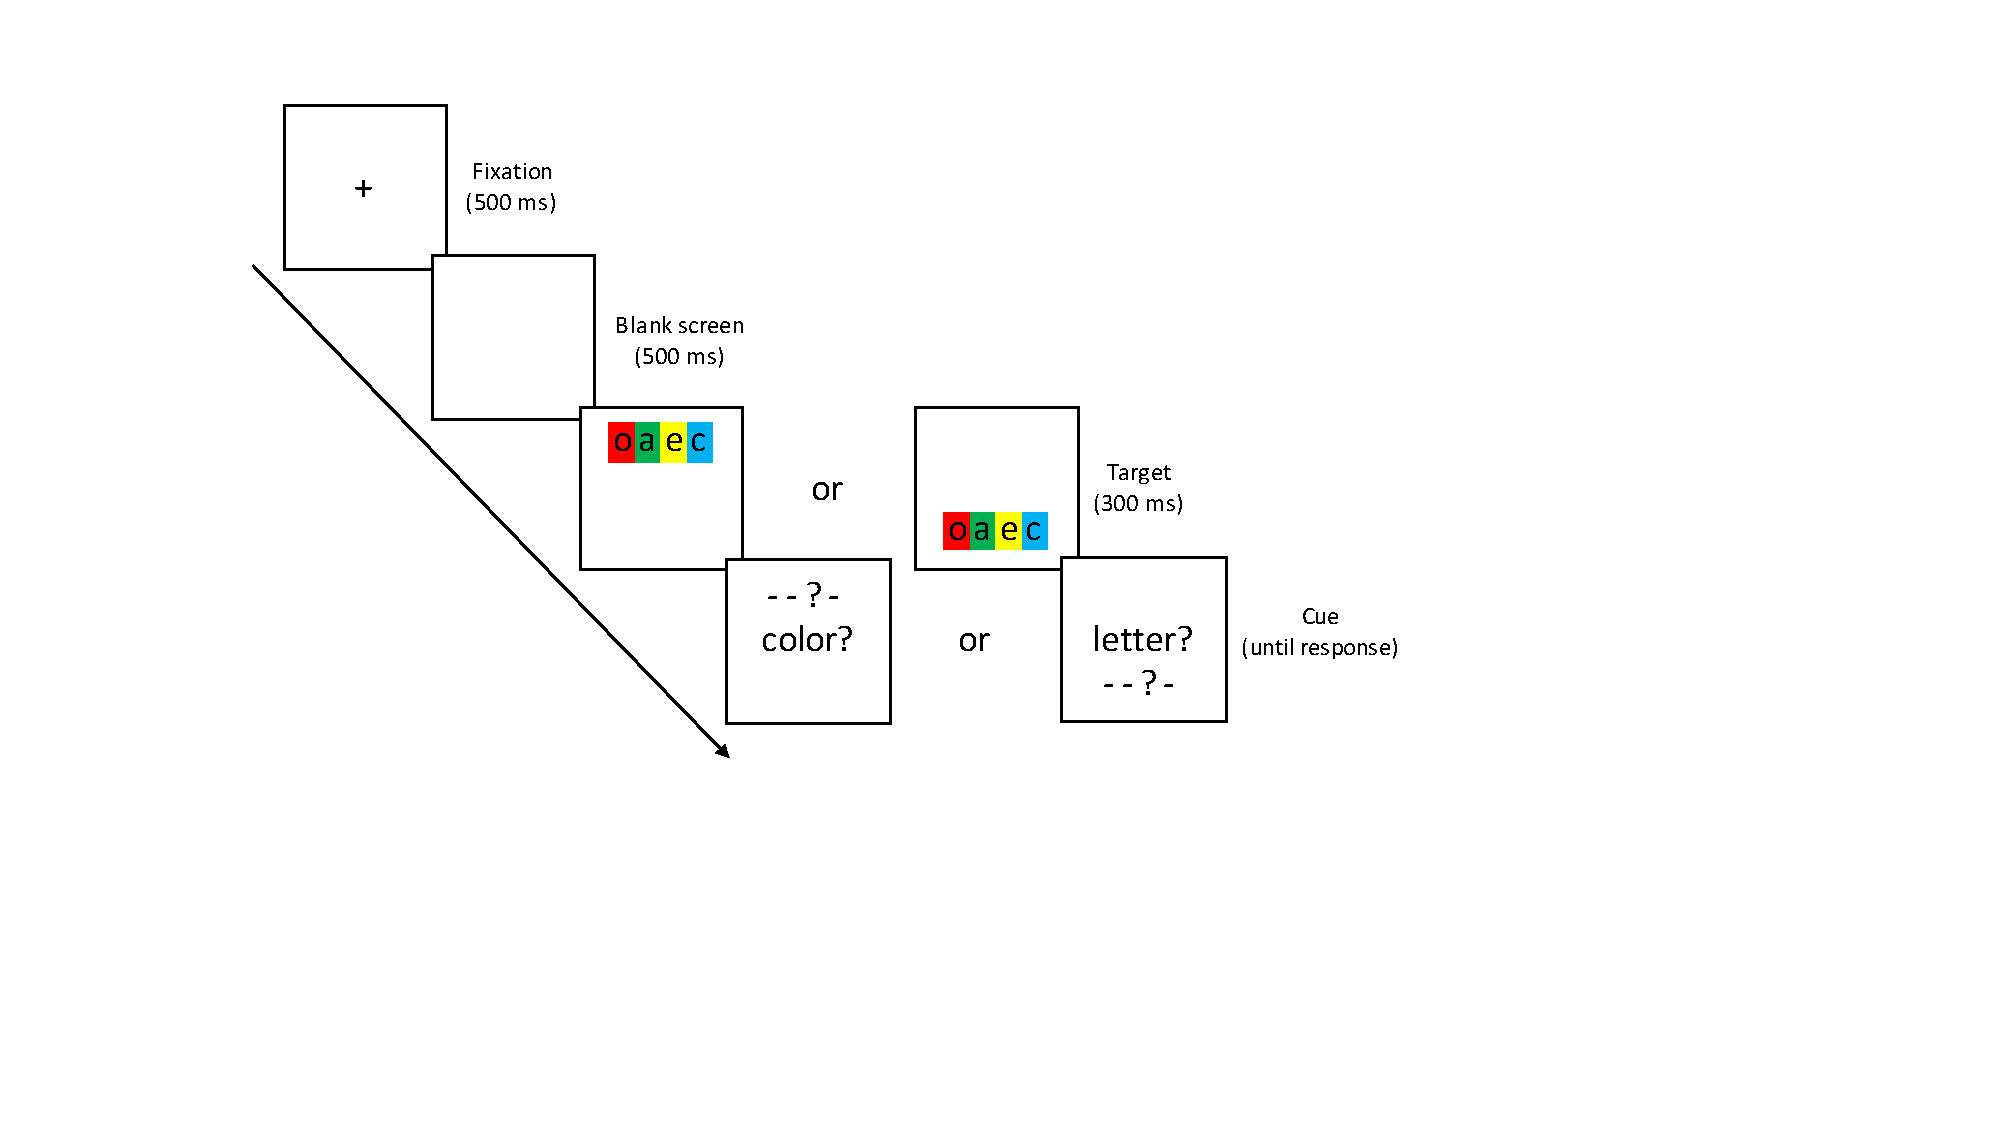
\includegraphics[width=5in]{figures/ICfigure1.pdf}
  \caption{Illustration of the trial sequence for all experiments.}
  \caption*{Note that the target could appear above or below the fixation. The identity cue ("Color?" or "Letter?") always appeared in the center of the screen while the position cue ("- - ? -") always appeared in the same location as the target. Participants were instructed to report either the letter or color in the cued position.}

  \label{IC_figure1}
\end{figure}

\hypertarget{methods}{%
\subsection{Methods}\label{methods}}

\hypertarget{subjects}{%
\subsubsection{Subjects}\label{subjects}}

All subjects were Brooklyn College undergraduate students (approximately
ages 18-22) who participated for course credit. Twenty subjects
completed Experiment 1 and all were included in the analysis.

\hypertarget{apparatus-stimuli}{%
\subsubsection{Apparatus \& Stimuli}\label{apparatus-stimuli}}

All experiments were programmed using LiveCode 7.0. The target stimuli
consisted of four lower-case letters (o, e, c, and a) superimposed on
four colored squares (red, green, blue, and yellow). The relative
positions of letters and colors on each trial were randomly chosen from
all possible letter/color permutations. The background was black and
stimuli were presented either above or below the fixation on a dark gray
rectangle.

The keyboard was labeled to indicate the four letters and four color
responses required. The keys A, S, D, and F were relabeled to A, O, E,
and C respectively; and, the keys H, J, K, and L were relabeled as red,
blue, green, and yellow, respectively.

\hypertarget{design}{%
\subsubsection{Design}\label{design}}

Experiment 1 used a 2x2 within-subjects design with cue validity (75\%
vs.~25\%) and task (color identification vs.~letter identification) as
factors. There were 480 trials in Experiment 1. One location (randomly
assigned as above or below the fixation) consisted of 75\% color
identification trials (160 trials) and 25\% letter identification trials
(80 trials) while the other location consisted of 75\% letter
identification trials and 25\% color identification trials. The trial
sequence was randomized and presented in an intermixed fashion for each
subject.

\hypertarget{procedure}{%
\subsubsection{Procedure}\label{procedure}}

Each subject read a brief overview about the stimuli they would be
presented and the types of responses required before signing a consent
form. Subjects were instructed to remember the locations of both the
colors and letters. Immediately following the target stimulus, a cue
would indicate the to-be-identified target, which could be a letter or a
color, located in any of the four positions.

Each trial began with a white fixation-cross presented in the center of
the screen for 500 ms followed by a blank screen for 500 ms. Next, the
target stimulus containing the four letters and four colors appeared for
300 ms followed immediately by the instructions for which stimulus to
identify. The dimension of the to-be-identified stimulus was indicated
by the words ``Letter?'' or ``Color?'' presented in the center of the
screen and its location was indicated by three dashes and a question
mark (i.e., ``- - ? -'') presented in the same location as the target
stimulus (see Figure \ref{IC_figure1}). For example, ``Letter?'' and ``?
- - -'' would indicate the letter located in the first position. No
accuracy feedback was given following a response and the next trial
began automatically. A mandatory 30-second break was given every 120
trials.

\begin{table}[htbp]
\caption{Mean correct color and letter identification response latencies, standard errors, and accuracy rates for all experiments.}
\label{IC_table}
\centering
\begin{tabular}{cccccccccc}
 & & & & \multicolumn{2}{c}{Training Phase} & \multicolumn{4}{c}{Mixed Phase} \\
\cmidrule(rl){5-6}
\cmidrule(rl){7-10}
 & & & & \multicolumn{2}{c}{100\%} & \multicolumn{2}{c}{75\%} & \multicolumn{2}{c}{25\%}  \\
\cmidrule(rl){5-6}
\cmidrule(rl){7-8}
\cmidrule(rl){9-10}
 & & \multicolumn{1}{c}{Task} & & \multicolumn{1}{c}{M} & \multicolumn{1}{c}{SE} & \multicolumn{1}{c}{M} & \multicolumn{1}{c}{SE} & \multicolumn{1}{c}{M} & \multicolumn{1}{c}{SE} \\
\midrule
\multicolumn{2}{l}{\textbf{Exp. 1}}  &   &    &     &     &    &  & & \\
& & \multicolumn{1}{c}{Color} & \multicolumn{1}{c}{ACC} & \multicolumn{1}{c}{-} & \multicolumn{1}{c}{-} & \multicolumn{1}{c}{64.56} & \multicolumn{1}{c}{3.58} & \multicolumn{1}{c}{63.32} & \multicolumn{1}{c}{3.63} \\
& & & \multicolumn{1}{c}{RT} & \multicolumn{1}{c}{-} & \multicolumn{1}{c}{-} & \multicolumn{1}{c}{1611} & \multicolumn{1}{c}{70} & \multicolumn{1}{c}{1606} & \multicolumn{1}{c}{68} \\
& & \multicolumn{1}{c}{Letter} & \multicolumn{1}{c}{ACC} & \multicolumn{1}{c}{-} & \multicolumn{1}{c}{-} & \multicolumn{1}{c}{61.84} & \multicolumn{1}{c}{3.56} & \multicolumn{1}{c}{62.17} & \multicolumn{1}{c}{3.35} \\
& & & \multicolumn{1}{c}{RT} & \multicolumn{1}{c}{-} & \multicolumn{1}{c}{-} & \multicolumn{1}{c}{1824} & \multicolumn{1}{c}{83} & \multicolumn{1}{c}{1858} & \multicolumn{1}{c}{90} \\
\cmidrule(l){2-10}
 &  & & & & & & & & \\
\multicolumn{2}{l}{\textbf{Exp. 2}}  &   &    &     &     &    &  & & \\
& & \multicolumn{1}{c}{Color} & \multicolumn{1}{c}{ACC} & \multicolumn{1}{c}{75.02} & \multicolumn{1}{c}{3.55} & \multicolumn{1}{c}{64.81} & \multicolumn{1}{c}{4.36} & \multicolumn{1}{c}{63.36} & \multicolumn{1}{c}{4.71} \\
& & & \multicolumn{1}{c}{RT} & \multicolumn{1}{c}{1152} & \multicolumn{1}{c}{47} & \multicolumn{1}{c}{1510} & \multicolumn{1}{c}{59} & \multicolumn{1}{c}{1556} & \multicolumn{1}{c}{67} \\
& & \multicolumn{1}{c}{Letter} & \multicolumn{1}{c}{ACC} & \multicolumn{1}{c}{77.11} & \multicolumn{1}{c}{3.23} & \multicolumn{1}{c}{58.31} & \multicolumn{1}{c}{3.4} & \multicolumn{1}{c}{59.09} & \multicolumn{1}{c}{3.88} \\
& & & \multicolumn{1}{c}{RT} & \multicolumn{1}{c}{1309} & \multicolumn{1}{c}{61} & \multicolumn{1}{c}{1707} & \multicolumn{1}{c}{80} & \multicolumn{1}{c}{1711} & \multicolumn{1}{c}{83} \\
\cmidrule(l){2-10}
& & & & & & & & & \\
\multicolumn{2}{l}{\textbf{Exp. 3}}  &   &    &     &     &    &  & & \\
& & \multicolumn{1}{c}{Color} & \multicolumn{1}{c}{ACC} & \multicolumn{1}{c}{79.83} & \multicolumn{1}{c}{3.08} & \multicolumn{1}{c}{67.59} & \multicolumn{1}{c}{4.65} & \multicolumn{1}{c}{56.62} & \multicolumn{1}{c}{4.91} \\
& & & \multicolumn{1}{c}{RT} & \multicolumn{1}{c}{1318} & \multicolumn{1}{c}{61} & \multicolumn{1}{c}{1595} & \multicolumn{1}{c}{58} & \multicolumn{1}{c}{1687} & \multicolumn{1}{c}{62} \\
& & \multicolumn{1}{c}{Letter} & \multicolumn{1}{c}{ACC} & \multicolumn{1}{c}{81.99} & \multicolumn{1}{c}{2.54} & \multicolumn{1}{c}{65.56} & \multicolumn{1}{c}{3.55} & \multicolumn{1}{c}{56.62} & \multicolumn{1}{c}{5.13} \\
& & & \multicolumn{1}{c}{RT} & \multicolumn{1}{c}{1560} & \multicolumn{1}{c}{96} & \multicolumn{1}{c}{1751} & \multicolumn{1}{c}{64} & \multicolumn{1}{c}{1858} & \multicolumn{1}{c}{87} \\
\cmidrule(l){2-10}
 & & & & & & & & & \\
\multicolumn{2}{l}{\textbf{Exp. 4}}  &   &    &     &     &    &  & & \\
& \multicolumn{1}{l}{Trained Context} & \multicolumn{1}{c}{Color} & \multicolumn{1}{c}{ACC} & \multicolumn{1}{c}{67.71} & \multicolumn{1}{c}{4} & \multicolumn{1}{c}{58.4} & \multicolumn{1}{c}{4.34} & \multicolumn{1}{c}{45} & \multicolumn{1}{c}{4.91} \\
& & & \multicolumn{1}{c}{RT} & \multicolumn{1}{c}{1519} & \multicolumn{1}{c}{80} & \multicolumn{1}{c}{1524} & \multicolumn{1}{c}{52} & \multicolumn{1}{c}{1596} & \multicolumn{1}{c}{52} \\
& & \multicolumn{1}{c}{Letter} & \multicolumn{1}{c}{ACC} & \multicolumn{1}{c}{77.81} & \multicolumn{1}{c}{4.14} & \multicolumn{1}{c}{56.04} & \multicolumn{1}{c}{4.52} & \multicolumn{1}{c}{48.12} & \multicolumn{1}{c}{5.39} \\
& & & \multicolumn{1}{c}{RT} & \multicolumn{1}{c}{1686} & \multicolumn{1}{c}{90} & \multicolumn{1}{c}{1625} & \multicolumn{1}{c}{43} & \multicolumn{1}{c}{1620} & \multicolumn{1}{c}{74} \\
\cmidrule(rl){3-10}
& \multicolumn{1}{l}{Reversed Context} & \multicolumn{1}{c}{Color} & \multicolumn{1}{c}{ACC} & \multicolumn{1}{c}{-} & \multicolumn{1}{c}{-} & \multicolumn{1}{c}{56.53} & \multicolumn{1}{c}{4.93} & \multicolumn{1}{c}{51.88} & \multicolumn{1}{c}{4.96} \\
& & & \multicolumn{1}{c}{RT} & \multicolumn{1}{c}{-} & \multicolumn{1}{c}{-} & \multicolumn{1}{c}{1489} & \multicolumn{1}{c}{31} & \multicolumn{1}{c}{1526} & \multicolumn{1}{c}{61} \\
& & \multicolumn{1}{c}{Letter} & \multicolumn{1}{c}{ACC} & \multicolumn{1}{c}{-} & \multicolumn{1}{c}{-} & \multicolumn{1}{c}{52.01} & \multicolumn{1}{c}{4.46} & \multicolumn{1}{c}{47.08} & \multicolumn{1}{c}{5.17} \\
& & & \multicolumn{1}{c}{RT} & \multicolumn{1}{c}{-} & \multicolumn{1}{c}{-} & \multicolumn{1}{c}{1607} & \multicolumn{1}{c}{36} & \multicolumn{1}{c}{1616} & \multicolumn{1}{c}{60} \\
 & & & & & & & & & \\
\bottomrule
\multicolumn{10}{l}{\textit{Note}: RT = Reaction Time (ms);  ACC = Accuracy (\%);  M = Mean; SE = } \\
\multicolumn{10}{l}{Standard Error;  100\%\textbackslash 75\%\textbackslash 25\% = Cue Validity.} \\
\end{tabular}%
\end{table}

\hypertarget{results}{%
\subsection{Results}\label{results}}

Overall identification accuracy was fairly low with an average accuracy
of 63\%, though subjects were well above chance (25\%). Given the low
accuracy scores, a response time analysis was inappropriate as nearly
40\% of trials would have been removed from the analysis resulting in
insufficient cell sizes. Furthermore, accuracy was well below ceiling
levels of performance and therefore, would be sensitive to improvements
in performance. Mean RTs and accuracy scores for all experiments are
displayed in Table \ref{IC_table}.

Mean accuracy scores for each subject in each condition were submitted
to a repeated-measures ANOVA with cue validity (75\% vs.~25\%) and task
(color identification vs.~letter identification) as factors. Mean
accuracy rates collapsed across subjects are presented in Figure
\ref{IC_figure2}.

Both main effects for cue validity, \(F(1, 19) = 0.21\),
\(\mathit{MSE} = 19.70\), \(p = .654\), \(\hat{\eta}^2_p = .011\), and
task \(F(1, 19) = 0.49\), \(\mathit{MSE} = 152.59\), \(p = .492\),
\(\hat{\eta}^2_p = .025\), were non-significant. Additionally, the
two-way interaction between cue validity and task was also
non-significant, \(F(1, 19) = 0.44\), \(\mathit{MSE} = 28.19\),
\(p = .517\), \(\hat{\eta}^2_p = .022\). Accuracy was not significantly
better for targets presented in their valid versus invalid locations.

\begin{figure}
  \centering
  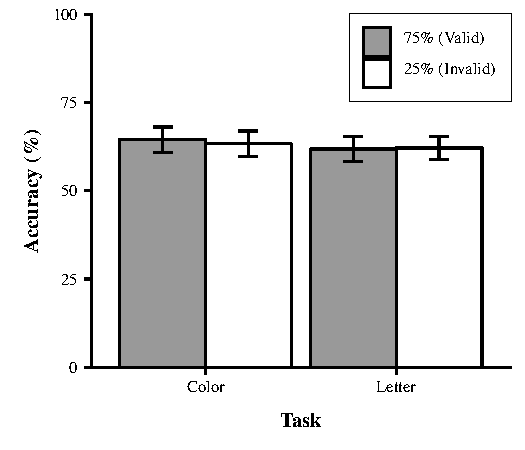
\includegraphics[height=3in]{figures/ICfigure2.pdf}
  \caption{Results from Experiment 1}
  \caption*{Accuracy scores (\%) for color and letter identification trials as a function of location cue validity.}
  \label{IC_figure2}
\end{figure}

\hypertarget{discussion}{%
\subsection{Discussion}\label{discussion}}

Experiment 1 failed to demonstrate context-specific control over
priorities for sampling from color vs.~letter dimensions in briefly
presented displays. Specifically, identification performance did not
vary as a function of location cue validity. The absence of contextual
control occurred despite the significant amount of errors made in all
locations. So, although there was an opportunity for adaptive learning
processes to modify attentional priorities based on error signals (in
this case, the subjective appraisals of performance), those processes
did not appear to influence performance. We cannot rule out whether or
not additional practice was necessary for contextual control to develop;
however, it clearly did not develop with amounts of practice sufficient
to produce contextual control in related procedures.

One possibility is that subjects did not attempt to intentionally change
attentional priorities for sampling from color and letter dimensions
between location contexts, and instead adopted a ``sample-everything''
strategy. This strategy would not prioritize one dimension over another,
but would instead involve attempting to register as many details about
both dimensions as possible. If subjects were employing such an
experiment-wide indiscriminate sampling strategy, then their memory
record would not be populated with instances preserving different
attentional priorities between contexts. Experiment 2 was designed to
populate the memory record with traces where attentional priorities were
modified between contexts.

\hypertarget{experiment-2}{%
\section{Experiment 2}\label{experiment-2}}

\begin{figure}
  \centering
  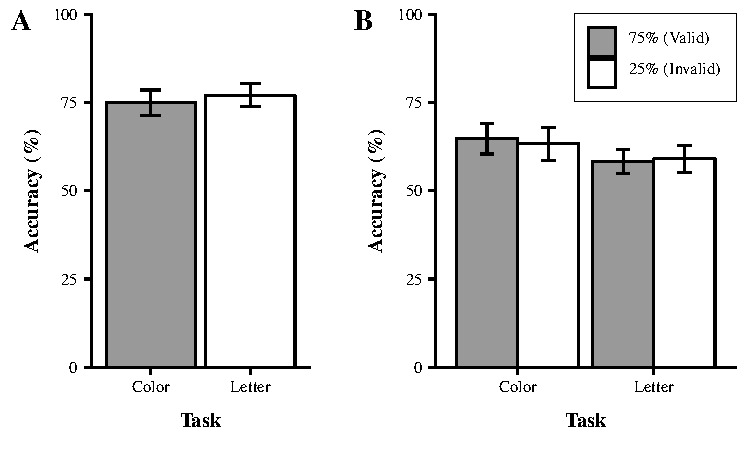
\includegraphics[height=3in]{figures/ICfigure3.pdf}
  \caption{Results from Experiment 2}
  \caption*{Results for the Training Phase (left) and Mixed Phase (right) from Experiment 2. Accuracy scores (\%) for color and letter identification trials as a
function of location cue validity.}
  \label{IC_figure3}
\end{figure}

The memory-driven account proposes that attentional processing details
are stored in individual memory traces. Contextual control is then the
result of the cue-driven retrieval and reinstatement of prior
attentional priorities (Crump, 2016; Crump and Milliken, 2009; Crump et
al., 2006, 2008). One interpretation of the absence of contextual
control in experiment one was the possibility that subjects were
adopting the very same ``sample everything'' strategy in both locations.
As a result, the locations may still be operating as effective cues, but
they may be cuing the very same attentional control settings in both
locations. The purpose of Experiment two was to establish a history of
differential attentional processing in each location. This was achieved
by including a blocked practice phase prior to the mixed trial phase.
The practice phase consisted of a block of trials where a single
identification task (e.g., color) was paired consistently with one
location, followed by another block where the other identification task
(e.g., letter) was paired consistently with the other location. Subjects
were informed about the blocked practice phase and mixed phase
experimental structure, but were not informed about the proportion
manipulations.

Proportion congruent designs sometimes include a blocked practice phase
to achieve context-specific attentional control. For example, Lehle and
Hübner (2008) could only demonstrate contextual control over flanker
effects when subjects received blocked practice first (see also Crump,
2016). This is consistent with the memory-driven account which requires
a history of experiences where different attentional priorities were
deployed in different situations. The blocked practice phase would allow
subjects to adopt dimension-specific sampling strategies, and the mixed
phase would allow us to test whether this training is required for
producing contextual control.

\hypertarget{methods-1}{%
\subsection{Methods}\label{methods-1}}

\hypertarget{subjects-1}{%
\subsubsection{Subjects}\label{subjects-1}}

All subjects were Brooklyn College undergraduate students (approximately
ages 18-22) who participated in this study for course credit. Twenty-one
subjects completed Experiment 2.

\hypertarget{apparatus-stimuli-1}{%
\subsubsection{Apparatus \& Stimuli}\label{apparatus-stimuli-1}}

The apparatus and stimuli were identical to Experiment 1.

\hypertarget{design-1}{%
\subsubsection{Design}\label{design-1}}

The design was similar to Experiment 1 except that subjects completed a
blocked practice phase prior to the mixed phase. Experiment 2, therefore
involved a one-way within-subjects practice phase with task as a factor
(color identification vs.~letter identification) and a separate 2x2
within-subjects design for the mixed phase with cue validity (75\%
vs.~25\%) and task (color identification vs.~letter identification) as
factors. The high-proportion tasks assigned to each location (above or
below the fixation) were randomly assigned across subjects. The
locations assigned to each task in the blocked practice phase were kept
consistent with the validity manipulation in the mixed phase. For
example, if the above location was assigned to color during the block
phase, the same location was assigned to be 75\% color identification in
the mixed phase. Whether the first practice block involved the color or
letter location was randomly assigned across subjects.

There were a total of 512 trials. The first practice block included 128
trials, with all stimuli appearing in one location and requiring only
one identification task. The second block repeated this procedure with
the other location and identification task. The last two blocks (the
mixed phase) consisted of 128 trials each, with 50\% color and letter
identification trials occurring with equal probability above or below
the fixation. As with Experiment 1, one location (randomly assigned as
above or below the fixation) consisted of 75\% color identification
trials (96 trials) and 25\% letter identification trials (32 trials)
while the other location consisted of 75\% letter identification trials
and 25\% color identification trials. The trial sequence was randomized
for each subject.

\hypertarget{procedure-1}{%
\subsubsection{Procedure}\label{procedure-1}}

The procedure was identical to Experiment 1.

\hypertarget{results-1}{%
\subsection{Results}\label{results-1}}

Mean accuracy scores for each subject in each condition are displayed in
Figure \ref{IC_figure3}. Mean RTs and accuracy scores for all
experiments are displayed in Table 1.

\hypertarget{training-phase.}{%
\subsubsection{Training Phase.}\label{training-phase.}}

Mean accuracy scores for each subject were submitted to a
repeated-measures ANOVA with task (color identification vs.~letter
identification) as the sole factor. There was no significant difference
between mean accuracy in the color identification block (M = 74.6\%) and
the letter identification block (M = 76.6\%), \(F(1, 20) = 0.29\),
\(\mathit{MSE} = 159.68\), \(p = .597\), \(\hat{\eta}^2_p = .014\).

\hypertarget{mixed-phase.}{%
\subsubsection{Mixed Phase.}\label{mixed-phase.}}

Mean accuracy scores for each subject were submitted to a
repeated-measures ANOVA with cue validity (75\% vs.~25\%) and task
(color identification vs.~letter identification) as factors. Both main
effects for cue validity, \(F(1, 20) = 0.04\), \(\mathit{MSE} = 0.01\),
\(p = .847\), \(\hat{\eta}^2_p = .002\) and task, \(F(1, 20) = 1.96\),
\(\mathit{MSE} = 0.03\), \(p = .177\), \(\hat{\eta}^2_p = .089\) were
non-significant. The two-way interaction between cue validity and task
was also non-significant, \(F(1, 20) = 0.46\), \(\mathit{MSE} = 0.01\),
\(p = .505\), \(\hat{\eta}^2_p = .023\). Subjects performed equally well
on the valid and invalidly cued trials.

How performance compared between the mixed and training phases was also
of interest. To address this question, overall accuracy scores from the
mixed and training phases were submitted to a pairwise t-test and found
that subjects performed significantly better in the Training Phase (M =
76\%) than the Mixed Phase (M = 61\%), \(t(20) = -5.38\), \(p < .001\).

\hypertarget{discussion-1}{%
\subsection{Discussion}\label{discussion-1}}

Experiment 2 again failed to demonstrate context-specific control over
attentional priorities for sampling from color and letter dimensions in
briefly presented displays. As with Experiment 1, in the mixed phase
targets were not better identified on valid versus invalid trials.

However, accuracy was substantially better in the blocked practice phase
than the mixed phase. One interpretation of this finding is that
attentional priorities for sampling from letter vs.~color dimensions can
be set in a preparatory fashion, when subjects know in advance which
dimension will be cued. On this view, our blocked phase would have
successfully created a memory record that would be suitable for
producing contextual control. That is, each subject would have a history
of experiences where they prioritized the color dimension in one
location and the letter dimension in the other. Yet, there was no
evidence of contextual control in the mixed phase.

There are several possibilities for the absence of context-specific
effects. Increased accuracy in the blocked phase may not reflect changes
to attention, but could instead reflect general differences in task
difficulty between blocked and mixed phases. Perhaps contextual control
phenomena do not generalize to our bi-dimensional sampling task.
Finally, it is possible that contextual control can be interfered with
by intentional control. More specifically, even though subjects may have
learned to assign different attentional priorities in each location
during the blocked practice phase, when they were confronted with the
trial-to-trial uncertainty of the upcoming identification task in the
mixed phase, they may have intentionally deployed a
``sample-everything'' strategy, which could have superseded any
contextual influences over setting attentional priorities.

\hypertarget{experiment-3}{%
\section{Experiment 3}\label{experiment-3}}

Experiment 3 investigated the role of intentions in producing contextual
control. Subjects were made aware of the location-specific proportion
manipulation and explicitly instructed to adopt and maintain
differential attentional strategies in each location. Specifically,
subjects were instructed to attend more to the colors in the color
location and more to the letters in the letter location, as indicated by
the training phase. Importantly, subjects were instructed to maintain
the location-specific attentional priorities in the mixed phase. In this
way, we tested whether or not context-specific differences in
attentional priorities could be set by intentional means

\hypertarget{methods-2}{%
\subsection{Methods}\label{methods-2}}

\hypertarget{subjects-2}{%
\subsubsection{Subjects}\label{subjects-2}}

All subjects were Brooklyn College undergraduate students (approximately
ages 18-22) who participated in this study for course credit. A total of
20 subjects completed Experiment 3.

\hypertarget{apparatus-stimuli-2}{%
\subsubsection{Apparatus \& Stimuli}\label{apparatus-stimuli-2}}

The apparatus and stimuli were identical to the previous experiments.

\hypertarget{design-2}{%
\subsubsection{Design}\label{design-2}}

The design was identical to Experiment 2.

\hypertarget{procedure-2}{%
\subsubsection{Procedure}\label{procedure-2}}

The procedure was similar to Experiment 2, however in Experiment 3
subjects were made aware of the proportion manipulation and instructed
to follow explicit strategies consistent with the predictiveness of the
location cue. Specifically, they were instructed to maintain the
strategy of ``attend more to the letters in the letter location'' and
``attend more to the colors in the color location'' as defined by their
practice phase. In addition, they were told to do there best when they
were asked to identify a dimension that was inconsistent with the
strategy, but to continue the strategy.

\hypertarget{results-2}{%
\subsection{Results}\label{results-2}}

One concern with adopting this set of instructions was that subjects
would ignore the task cues and always respond with the high-proportion
task response set. For example, when the target display occurred in the
75\% letter location, subjects may ignore the cue that says ``Color?''
and respond with a letter every trial. To determine which subjects may
have adopted this strategy, we calculated the task accuracy for each
subject in each condition. The task accuracy reflects the proportion of
trials where a subject responded with one of the four appropriate
response keys (letters when asked for a letter and colors when asked for
a color) regardless of whether it was the correct response. Subjects
with less than 25\% task accuracy in any condition were not included in
the analysis. This criterion was applied to all remaining analyses. For
Experiment 3, this eliminated three subjects. Mean task accuracy for the
remaining subjects was 96\%.

Mean accuracy scores for each subject in each condition are displayed in
Figure \ref{IC_figure4}. Mean RTs and accuracy scores for all
experiments are displayed in Table 1.

\hypertarget{training-phase}{%
\subsubsection{Training Phase}\label{training-phase}}

There was no significant difference between the mean accuracy in the
color identification block (M = 79.8\%) and the letter identification
block (M = 81.9\%), \(F(1, 16) = 0.61\), \(\mathit{MSE} = 64.60\),
\(p = .445\), \(\hat{\eta}^2_p = .037\).

\hypertarget{mixed-phase}{%
\subsubsection{Mixed Phase}\label{mixed-phase}}

Mean accuracy scores for each subject were submitted to a
repeated-measures ANOVA with cue validity (75\% vs.~25\%) and task
(color identification vs.~letter identification) as factors. The
critical main effect of cue validity was significant
\(F(1, 16) = 14.34\), \(\mathit{MSE} = 0.01\), \(p = .002\),
\(\hat{\eta}^2_p = .473\). Additionally, the main effect for task was
non-significant \(F(1, 16) = 0.06\), \(\mathit{MSE} = 0.03\),
\(p = .808\), \(\hat{\eta}^2_p = .004\), and the two-way interaction
between cue validity and task was non-significant \(F(1, 16) = 0.28\),
\(\mathit{MSE} = 0.01\), \(p = .605\), \(\hat{\eta}^2_p = .017\).
Subjects therefore performed better for both letter and color targets on
valid than invalid trials.

\hypertarget{discussion-2}{%
\subsection{Discussion}\label{discussion-2}}

Experiment 3 successfully demonstrated that subjects can adjust
attentional priorities for sampling from letter versus color dimensions
between contexts in the mixed phase. It is possible that the adjustment
of attentional priorities reflected contextual control processes, but
they could also reflect rapid intentional control. That is, subjects
could simply be following task instructions to deliberately change their
attentional priorities in response to the location context in which a
display occurs.

\begin{figure}
  \centering
  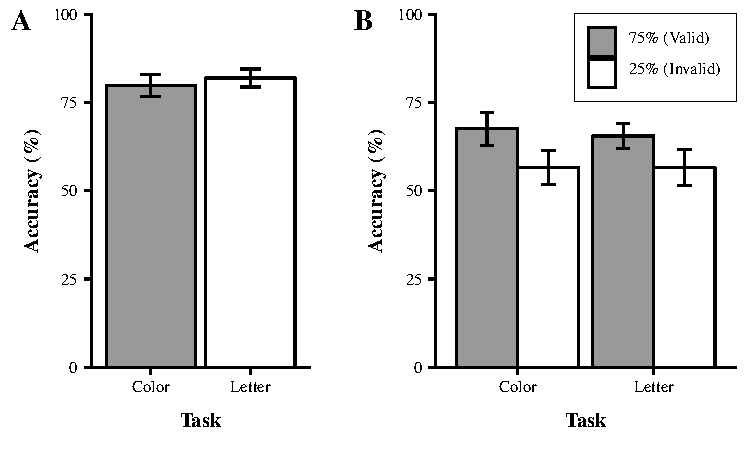
\includegraphics[height=3in]{figures/ICfigure4.pdf}
  \caption{Results from Experiment 3}
  \caption*{Results for the Training Phase (left) and Mixed Phase (right) from Experiment 3. Accuracy scores (\%) for color and letter identification trials as a
function of location cue validity.}
  \label{IC_figure4}
\end{figure}

\hypertarget{experiment-4}{%
\section{Experiment 4}\label{experiment-4}}

Experiment 4 used a process-dissociation type logic (Jacoby, 1991) to
isolate potential automatic and voluntary influences driving the
context-specific effects found in Experiment 3. Like Experiments 2 and
3, Experiment 4 included a blocked practice and a mixed phase. However,
the mixed phase contained two kinds of blocks that were either
consistent or inconsistent with training. In the consistent blocks, the
valid (75\%) locations for color and letter tasks were consistent with
training. In the inconsistent blocks, the valid locations were reversed
from those used in training. Additionally, subjects were instructed
throughout the experiment about which dimension should be attended to in
each location. Subjects were always told which location was valid for
both tasks, and were always instructed to prioritize each task in its
respective predicted location for the current block. If the effects from
Experiment 3 are due solely to volition, then subjects should be able to
adjust their strategies appropriately even when those strategies are
assigned to locations that were inconsistent with training. If on the
other hand, subjects did form associations between location cues and
intentionally set attentional priorities, then reversing the
high-proportion tasks assigned to location contexts should interfere
with context-specific effects by acting against intentional influences.

\hypertarget{methods-3}{%
\subsection{Methods}\label{methods-3}}

\hypertarget{subjects-3}{%
\subsubsection{Subjects}\label{subjects-3}}

All subjects were Brooklyn College undergraduate students (approximately
ages 18-22) who participated in this study for course credit. Twenty-six
subjects completed Experiment 4.

\hypertarget{apparatus-stimuli-3}{%
\subsubsection{Apparatus \& Stimuli}\label{apparatus-stimuli-3}}

The apparatus and stimuli were identical to the previous experiments.

\hypertarget{design-3}{%
\subsubsection{Design}\label{design-3}}

The design was similar to Experiment 3 except that subjects completed
blocks of trials where the high-proportion locations were reversed. This
involved a practice phase with task as a factor (color identification
vs.~letter identification), and a separate 2x2x2 within-subjects design
for the mixed phase with cued validity (75\% vs.~25\%), task (color
identification vs.~letter identification) and test blocks (trained
context vs.~reversed context) as factors. The high-proportion tasks
assigned to each location (above or below the fixation) were randomly
assigned across subjects. The locations assigned to each high-proportion
task in the blocked practice phase were consistent with the trained
context blocks and reversed in the reversed context blocks.
Additionally, whether the first practice block involved the
high-proportion color or high-proportion letter location was also
randomly assigned across subjects.

There were 480 trials. The first practice block included 48 trials, with
all stimuli appearing in one location and requiring only one
identification task. The second block repeated this procedure with the
other location and other identification task. The mixed phase involved
four blocks of 96 trials with 50\% color and letter identification
trials occurring with equal probability above or below the fixation. One
location (randomly assigned to above or below the fixation) consisted of
75\% color identification trials and 25\% letter identification trials
while the other location consisted of 75\% letter identification trials
and 25\% color identification trials. The first and third blocks were
trained context blocks, in that the locations for the valid trials were
consistent with those during training. The second and fourth blocks were
reversed context blocks, in that the locations for the valid trials were
reversed from those in the training phase. The trial sequence was
randomized for each subject.

\hypertarget{procedure-3}{%
\subsubsection{Procedure}\label{procedure-3}}

The procedure was similar to Experiment 3, in that subjects were made
aware of the proportion manipulation and instructed to follow explicit
strategies to account for the predictiveness of the location cue.
However, every 96 trials, the prompt would instruct them to reverse
their strategies.

\hypertarget{results-3}{%
\subsection{Results}\label{results-3}}

As with Experiment 3, task accuracy was calculated for each subject and
those with less than 25\% were not included in the analysis.
Accordingly, six subjects were eliminated from the following analysis.
Mean task accuracy for the remaining subjects was 92\%. Mean accuracy
scores for each subject in each condition are displayed in Figure
\ref{IC_figure5}. Mean RTs and accuracy scores for all experiments are
displayed in Table 1.

\hypertarget{training-phase-1}{%
\subsubsection{Training phase}\label{training-phase-1}}

Accuracy was significantly better in the letter identification task (M =
77.8\%) than the letter identification block (M = 67.7\%),
\(F(1, 19) = 10.48\), \(\mathit{MSE} = 97.38\), \(p = .004\),
\(\hat{\eta}^2_p = .356\).

\hypertarget{mixed-phase-1}{%
\subsubsection{Mixed phase}\label{mixed-phase-1}}

Mean accuracy scores for each subject were submitted to a
repeated-measures ANOVA with cue validity (75\% vs.~25\%), task (color
identification vs.~letter identification) and test blocks (trained
context vs.~reversed context) as factors.

The three-way interaction between cue validity, task, and test blocks
was non-significant, \(F(1, 19) = 1.94\), \(\mathit{MSE} = 0.00\),
\(p = .180\), \(\hat{\eta}^2_p = .093\). However, the critical two-way
interaction between cue validity and test blocks was significant
\(F(1, 19) = 5.25\), \(\mathit{MSE} = 0.01\), \(p = .034\),
\(\hat{\eta}^2_p = .217\), showing that the validity effect was larger
during trained context test blocks compared to reversed context test
blocks. To further analyze the significant two-way interaction, task was
collapsed over and the reversed and trained context conditions were
analyzed separately. A separate analysis of the trained context revealed
significantly higher accuracy on valid (M = 57\%) than invalid (M =
47\%) trials, \(t(19) = 3.34\), \(p = .003\). The analysis of the
reversed context also showed higher accuracy on valid (M = 54\%) than
invalid (M = 50\%) trials, \(t(19) = 2.09\), \(p = .050\).

For the sake of completeness: The two-way interaction between cue
validity and task \(F(1, 19) = 1.00\), \(\mathit{MSE} = 0.01\),
\(p = .329\), \(\hat{\eta}^2_p = .050\), and task and test blocks, ,
were both non-significant. Finally, the main effect for cue validity was
significant, \(F(1, 19) = 9.85\), \(\mathit{MSE} = 0.02\), \(p = .005\),
\(\hat{\eta}^2_p = .341\), and the main effects for both task
\(F(1, 19) = 0.98\), \(\mathit{MSE} = 0.02\), \(p = .335\),
\(\hat{\eta}^2_p = .049\), and test blocks, \(F(1, 19) = 0.00\),
\(\mathit{MSE} = 0.01\), \(p = .991\), \(\hat{\eta}^2_p = .000\), were
non-significant.

\begin{figure}
  \centering
  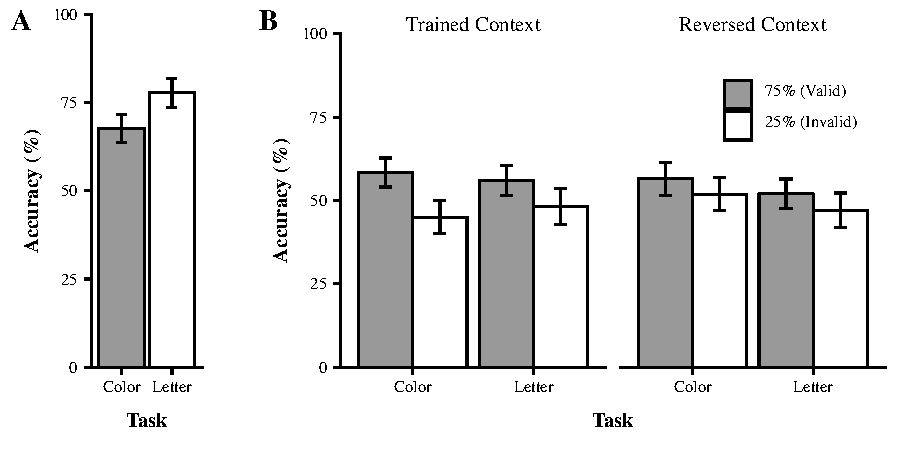
\includegraphics[height=3in]{figures/ICfigure5.pdf}
  \caption{Results from Experiment 4.}
  \caption*{Results for the Training Phase (left) and Mixed Phase (right) from Experiment 4. Accuracy scores (\%) for color and letter identification trials as a function of location cue validity.}
  \label{IC_figure5}
\end{figure}

\hypertarget{block-analysis}{%
\subsubsection{Block analysis}\label{block-analysis}}

Also of interest was whether the validity effects changed over the
course of the experiment. We divided the test trials in half, examining
the validity effects in the first half of the test trials (comprised of
the first trained and reversed context blocks) and the second half
(comprised of the second trained and reversed context blocks). A visual
inspection of the results displayed in Figure \ref{IC_figure6} suggest a
validity effect for the trained context block but not the reversed
context block in the first half, and no validity effects for either the
trained or reversed context blocks in the second half. This result was
confirmed in the following statistical analyses. For the sake of
brevity, only the critical tests are reported.

Mean accuracy scores were submitted to a repeated-measures ANOVA with
test half (first half vs.~second half), cue validity (75\% vs.~25\%),
task (color identification vs.~letter identification), and test block
(trained context vs.~reversed context) as factors. The four-way
interaction was non-significant, \(F(1, 19) = 0.01\),
\(\mathit{MSE} = 0.01\), \(p = .926\), \(\hat{\eta}^2_p = .000\).
However, the critical three-way interaction between test half, test
block, and cue validity was significant, \(F(1, 19) = 7.55\),
\(\mathit{MSE} = 0.02\), \(p = .013\), \(\hat{\eta}^2_p = .284\).

To probe the three-way interaction, each test half (first and second)
was analyzed separately, collapsing over task. Mean accuracy scores for
each test half were submitted to a repeated measures ANOVA with cue
validity (75\% vs.~25\%) and test block (trained context vs.~reversed
context) as factors.

First, we analyzed the first half and found a significant two-way
interaction between cue validity and test block, \(F(1, 19) = 18.27\),
\(\mathit{MSE} = 0.01\), \(p < .001\), \(\hat{\eta}^2_p = .490\).
Further analyses of the simple effects revealed significantly higher
accuracy in the 75\% (valid) trials (M = 57\%) as compared to the 25\%
(invalid) trials (M = 37\%) for the trained context, \(t(19) = 4.62\),
\(p < .001\), and no significant difference between accuracy scores in
the 75\% (valid) and 25\% (invalid) trials for the reversed context,
\(t(19) = 1.62\), \(p = .121\).

An analysis of the second half revealed no significant two-way
interaction between cue validity and test block, . The main effect of
cue validity was also non-significant, \(F(1, 19) = 2.23\),
\(\mathit{MSE} = 0.01\), \(p = .152\), \(\hat{\eta}^2_p = .105\). The
main effect of test block however, was significant, \(F(1, 19) = 8.63\),
\(\mathit{MSE} = 0.01\), \(p = .008\), \(\hat{\eta}^2_p = .312\).

To summarize, we analyzed the first and second halves of the test trials
separately and found a significant validity effect for the trained
context and no validity effect for the reversed context in the first
half of the test trials. For the second half we found no significant
validity effects across both the trained and reverse context test
blocks.

\begin{figure}
  \centering
  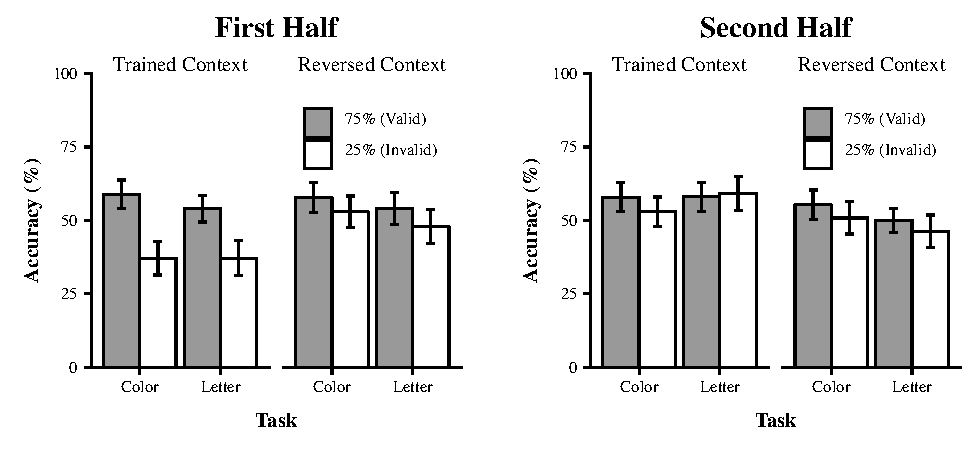
\includegraphics[height=3in]{figures/ICfigure6.pdf}
  \caption{Results from Experiment 4: Block Analysis.}
  \caption*{Results from Experiment 4 for the first (left) and second (right) halves of the Mixed Phase. Accuracy scores (\%) as a function of task (color vs. letter), location cue validity (75\% vs. 25\%) and test blocks (trained context vs. reversed context).}
  \label{IC_figure6}
\end{figure}

\hypertarget{discussion-3}{%
\subsection{Discussion}\label{discussion-3}}

The results of Experiment 4 replicate the general findings of Experiment
3 showing that identification accuracy was higher on valid than invalid
trials. The critical finding was that the validity effect depended on
the nature of the test block. The validity effect was larger on trained
context blocks compared to reversed context blocks. Trained context
blocks assigned the 75\% color and 75\% letter task locations to the
same locations used for each task during blocked practice. The reversed
context blocks flipped the assignment with respect to blocked practice.
As a reminder, prior to and during each test block subjects were always
told which location predicted each task. They were also instructed to
attend more to color in the location that predicted the color task, and
more to letters in the location that predicted the letter task. If the
validity effect was entirely driven by a flexible intentional control
process, then we expected that process to produce equivalent validity
effects regardless of whether the test block was consistent or reversed
from training. Instead, we found smaller validity effects in the
reversed context test blocks. One interpretation of this finding is that
the associations between contextual cues and attentional strategies
formed during training interfered with the deployment of intentional
strategies during the reverse context test blocks. On this view, the
results from Experiments 3 and 4 are not due solely to voluntary shifts
in attentional prioritization, but also reflect some contribution of
contextual control over setting of attentional priorities.

We also found significant changes in the validity effects from the first
to second half of the test blocks. Specifically, there was only a
validity effect in the first block of the trained context trials and
there were no significant validity effects for the reversed context
trials in either block. Our purpose in running Experiment 4 was to
determine whether the results from Experiment 3 could be accounted for
solely on the basis of volitional shifts in attentional prioritization.
The block analysis then provides even less support for this idea that
subjects could flexibly shift attentional priorities in the reversed
context blocks because there was no evidence for any validity effect
within each reversed block when analyzed separately. However, our design
consisted of a fixed order of test blocks (trained, reversed, trained,
reversed) and we only found validity effects in the first block. One
possibility is that subjects were unable to continually deploy
instructed strategies. Perhaps subjects lacked motivation to continue
applying the instructed strategies or they were motivated but only had
available resources to apply the effortful strategies for a short period
of time. On this view, subjects could voluntarily shift attentional
priorities but chose not to or were unable to maintain voluntary control
over longer periods. However, we note that accuracy in general increased
across blocks, which suggests that subjects became more motivated to
perform well in the task.

Alternatively, the finding that the validity effects were only evident
in the first test blocks could also reflect some contribution of
contextual control over setting of attentional priorities. It is clear
that in the first test block subjects did adopt the trained attentional
strategy, but then failed to adopt the reversed strategy in the second
block. One interpretation is that training provided the needed
experiential support for enacting the strategy, and when that support
was missing (for the reversed context blocks) strategic control was not
possible. Similarly, the disappearance of the validity effect could be
due to the fact that associations formed during training were
extinguished during the mixed phase which involved many new trial types
that were inconsistent with training. This interpretation fits with
previous findings that effectively applying an attentional strategy for
ignoring a distractor requires experiential learning, or practice with
ignoring the distractor (Vecera et al., 2014). For example, Cunningham
and Egeth (2016) examined whether subjects could make use of a pre-cue
signaling the identity of an upcoming distractor for the purposes of
ignoring the irrelevant feature when it appeared. They found that
subjects learned to ignore distractors that were preceded by a
consistent cue that always signaled the same distracting feature across
trials. However, when the pre-cue signaled different distracting
features across trials participants failed to benefit from the pre-cue
for the purpose of ignoring the signaled distractor. Our results are
similar in that subjects were able to transfer their learning from the
practice blocks to the first test block which was mostly consistent with
training. However, across test blocks attentional sampling demands
became increasingly inconsistent with practice and prevented transfer of
learning from the practice phase to test block performance.

\hypertarget{general-discussion}{%
\section{General Discussion}\label{general-discussion}}

In experiment one, one location involved 75\% color and 25\% letter
identification trials and the other involved 75\% letter and 25\% color
identification trials. Despite the fact that location predicted the
likely task on each trial, we found no evidence of contextual control.
Specifically, identification performance on validly cued trials was not
different from invalidly cued trials. The automatic adaptation accounts
posit learning processes sensitive to error- or conflict-driven signals;
however, no evidence of contextual control was found in Experiment 1
despite the poor accuracy that should allow for such learning processes
to operate. One explanation of the absence of contextual control was the
suggestion that subjects adopted a ``sample everything'' strategy on
every trial, and learned associations between location contexts and the
attentional priorities assigned by the ``sample everything'' strategy.

In experiment two, the mixed phase was preceded by a blocked training
phase where each identification task was performed consistently in a
particular location. The blocked phase was included to ensure that
subjects had experiences with deploying different attentional priorities
between contexts. We found better identification performance in the
blocked than the mixed phases. However, there was no validity effect in
the mixed phase, indicating no evidence of contextual control. Although
there was evidence that subjects did learn to assign different
attentional priorities in the different contexts during the blocked
practice, this learning apparently failed to transfer to control setting
of attentional priorities in the mixed phase. One reason for the absence
of contextual control in the mixed phase was that subjects again decided
to adopt the ``sample everything'' strategy which could have overridden
the ability of contextual cues to set attentional priorities.

In experiment three, we repeated the same design as experiment two, but
made subjects aware of the validity manipulation and gave them
instructions to attend more to color information in the 75\% color
location, and more to letter information in the 75\% letter location.
The major finding was the presence of a validity effect in the mixed
phase, indicating that subjects were capable of assigning different
attentional priorities between locations. However, it remained unclear
whether this effect was mediated by cue-driven or intentional influences
over setting of attentional priorities.

In experiment four, we included new test blocks in the mixed phase where
the valid locations for the color and letter tasks were consistent or
reversed from training. The critical finding was a larger validity
effect when the locations were consistent rather than reversed from
training. Here, the maintenance of voluntary attentional strategies was
impaired when the strategies were inconsistent with the attentional
priorities cued by location contexts established during training. This
finding suggests that the validity effect in the mixed phase was not
entirely driven by a flexible intentional process capable of setting
attentional priorities according to instructions, but also reflects a
contribution from contextual influences that control the setting of
attentional priorities in a cue-driven fashion.

One general aim of the present work was to test guiding principles of
contextual control by using a novel bi-dimensional sampling task. We
found some cases where contextual control was not acquired or expressed
in performance, and some cases where contextual control appeared to
depend on previous experience with deploying different strategies for
setting attentional priorities between contexts. We now turn to a
discussion of the roles of awareness and intention in promoting
contextual control, as well as a number of task differences between our
procedure and previous ones that may explain the presence and absence of
contextual control across our experiments.

Our findings depart from previous work showing that contextual control
develops without awareness and intention. We consider two perspectives
about how our findings relate to previous work. First, we may have found
an exceptional case where contextual control does depend on experiences
with intentionally adopting different attentional priorities in
different contexts. On this view, contextual control can develop with or
without intention, and whether or not contextual control relies on
intention would be task-dependent.

Second, we consider the possibility that prior demonstrations of CSPC
effects did depend on experiences with intentionally adopting different
attentional priorities between contexts. A common finding in Stroop and
flanker variants is that subjects are not aware of the CSPC
manipulation. One interpretation of this finding is that subjects who
were not aware of the manipulation did not intentionally use contextual
cues to adopt different attentional priorities. However, we assume that
subjects were always intentionally controlling attention priorities at
the level of specific items, and that individual stimuli provoke
subjects to adopt particular attentional priorities appropriate to the
stimulus and task at hand. Consider the item-specific strategies adopted
by a subject in CSPC Stroop task who is unaware of the CSPC
manipulation, but who is following instructions to respond to a color
dimension as quickly and accurately as possible. When a congruent item
is presented, subjects may actively assign more priority to the word
dimension because it matches with the correct color response. When an
incongruent item is presented, subjects may actively assign less
priority to the word dimensions because it does not match the correct
color response. In this way, subjects may have intentions for setting
attentional priorities at the item-specific level that can be exercised
on each trial regardless of whether they are aware of the
context-specific proportion congruent manipulation. As a result, the
attentional priorities resulting from intentional control at the
item-level could become associated with the contexts in which items
frequently occur, thereby leading to the development of contextual
control.

In order to entertain the view that intentional control does influence
the acquisition of contextual control across tasks, we also need to
consider discrepancies in the effectiveness of instructional
manipulations. We show that subjects can follow instructions to adopt
context-specific attentional priorities in the bi-dimensional sampling
task. However, similar instructional manipulations were not effective in
a CSPC Stroop task (Crump et al., 2008). Here, subjects were encouraged
to adopt context-specific attentional priorities in response to the
shape context of a target stimulus. Subjects were aware of the CSPC
manipulation and were instructed to adopt context-specific attentional
priorities; nevertheless, no evidence of contextual control was
obtained. One interpretation of this finding is that intentional control
is not sufficient for producing contextual control. However, it remains
unclear whether those subjects could follow the instructions. For
example, in their prime-probe Stroop task the subject was briefly
presented with a word that disappeared before the target color patch was
displayed in one of two shapes. The instruction was to use the shape cue
to rely more or less on the previous word to help with responding to the
color of the target. It is not clear how subjects would attempt to
retrospectively ignore the influence of an already presented word.
Therefore, intentional control may have failed to influence the
acquisition of contextual control in those tasks because subjects were
never engaging in context-specific intentional control to begin with. By
contrast, in the current task the instruction to attend more to the
colors versus the letters may be easier to communicate, more readily
understood, and easier to execute than instructions employed in prior
tasks.

Finally, there are critical differences between our task and those that
have previously demonstrated contextual control. Though the current
study suggests that intentional control may be a pre-requisite for the
acquisition of contextual control, these task differences could
potentially limit the generalizability of our findings and warrant
further discussion.

Contextual control has been observed in several interference tasks where
there is response conflict between target and distractor dimensions. In
contrast, there was no apparent response conflict between our color and
letter dimensions. Some theories of contextual control assume that the
presence of this conflict drives learning and mediates the acquisition
of contextual control (Blais et al., 2012; Botvinick et al., 2001;
Verguts and Notebaert, 2008, 2009). For example, Crump et al. (2008)
showed no CSPC effects in a Stroop task where subjects named words
rather than colors. If contextual control depends on the presence of
response conflict between target and distractor dimension, then the
absence of contextual control in experiments one and two could be due to
the absence of similar kinds of conflict in our task.

At the same time, we assume that our displays prompted ubiquitous
response competition on each trial. Target displays consisted of four
unique letters and colors and therefore on any given trial, eight
potential responses. Additionally, the total amount of response
competition could have been reduced substantially (from eight to four)
to the extent that contextual cues signaled selective processing of the
dimension that was usually probed in that location. On this view, if the
acquisition of contextual control is strongly related to the size of the
conflict signal, we would have expected rapid learning and strong
evidence for contextual control in our first experiments.

Alternatively, it is possible that the high degree of response conflict
prevented the acquisition of contextual control. Prior work has
demonstrated an absence of contextual control when subjects failed to
attend to contextual information. For example, Crump, Gong, and Milliken
(2006) could only find evidence for contextual control using shape cues
when subjects were given a secondary task that required them to
explicitly attend to the shapes. This suggests that contextual
information may need to be attended to and integrated with target
information in order for contextual control to develop. The high degree
of response conflict in our task may have limited the amount of
attention subjects could direct to the contextual features or caused a
failure in the stimulus-context integration process; both of which could
explain the absence of contextual control in our experiments.

The time-course of stimulus presentation relative to the contextual cues
may also influence the acquisition of contextual control. In our
experiments we always presented the target display simultaneously with
the contextual cue. Simultaneous presentation has been effective in
demonstrating contextual control in Stroop and flanker tasks (Bugg and
Crump, 2012). In general, prior work has not systematically explored how
the time-course of contextual cueing influences the effectiveness of the
cues. However, Reuss et al. (2014) presented the contextual cue either
prior to or simultaneously with the target and found contextual control
in both cases and Fischer et al. (2014) found contextual control
developed more rapidly when the location-context was cued prior to the
target. We could speculate however, that the effectiveness of the cue
changes as a function of the timing relationships and it is possible
that these changes are task-dependent. For example, simultaneous
presentations may be effective in a Stroop or flanker task, but
ineffective in a bi-dimensional sampling task such as ours. For this
reason, it is possible that the absence of contextual control in our
experiments was due to the fact that we used simultaneous presentations
rather than advance presentations. In general, systematic investigation
of time-course issues in any demonstration of contextual control is an
important topic for future work.

Numerous studies show that attentional priorities for processing
stimulus dimensions can be modulated by contextual cues (e.g., Corballis
and Gratton, 2003; Crump, 2016; Crump et al., 2006, 2008; Gough et al.,
2014; King et al., 2012). Furthermore, a growing body of literature has
demonstrated that awareness of experimental manipulations such as
dimensional-conflict, proportion of trial-types, and contextual cues,
are not required to produce such effects (e.g., Heinemann et al., 2009;
King et al., 2012; Panadero et al., 2015; Reuss et al., 2014; Sarmiento
et al., 2012). This lack of awareness has suggested that contextual
control can occur independent of a subject's intent. Our findings add to
this body of work and show one situation where intentional setting of
attentional priorities appears to be a pre-requisite for
context-specific control. Our experiments also show that principles from
theories of contextual control such as automatic error-driven learning,
and automatic retrieval of prior instances do not necessarily generalize
across tasks in a straightforward manner.

\FloatBarrier

\newpage
\fancyhead[L]{SINGLE EXPERIENCES WITH CONFLICT}
\fancyhead[R]{\thepage}
\fancyfoot[C]{}

\chapter{SINGLE EXPERIENCES WITH CONFLICT HAVE LONG-LASTING EFFECTS ON COGNITIVE CONTROL}

\hypertarget{preface-1}{%
\section{Preface}\label{preface-1}}

This chapter is reproduced from a published article in
\textit{Journal of Experimental Psychology: General} (for consistency, I
have adjusted the format of the manuscript for the thesis). The full
reference to the article:

\vspace{1.5em}

\noindent \textbf{Brosowsky, N.P.} \& Crump, M.J.C. (2018),
Memory-guided selective attention: Single experiences with conflict have
long-lasting effects on cognitive control. Journal of Experimental
Psychology: General , 147(8), 1134-1153.
\url{http://dx.doi.org/10.1037/xge0000431} \vspace{1.5em}

Chapter 3 presents a set of three experiments testing general principles
of the instance-based memory account. Two key assumptions that fall out
of the memory-based account are that (1) processing details from
individual experiences are stored in memory traces and (2) these memory
traces are stored for the long-term. Although the context-specific
proportion congruent phenomena are often taken as evidence for a
memory-based retrieval process, because a small set of items repeat
throughout the experiment there is no way to trace the changes in
performance back to any single prior experience. Here, we examined
whether single experiences can have long-term (4 to 319 intervening
trials) on selective attention.

Long-term item-specific effects have been demonstrated across a variety
of different cognitive control paradigms like negative priming and
task-switching, but has never been examined within the context of more
traditional selective attention paradigms like Stroop and flanker tasks.
However, the congruency sequence effect, a very common Stroop and
flanker phenonemon, demonstrates short-term single-trial effects, but is
not typically explained as the result of a memory-retrieval process.
Here, we used a large set of unique context items to determine whether a
single experience applying attentional control on an item can influence
a second presentation after many intervening trials. If so, we predicted
we would see a pattern of results similar to the congruency sequence
effect.

Across three experiments we found evidence that single experiences can
influence selective attention after many intervening trials (4 to 319).
However, we also note some boundary conditions, failing to find such
effects when the repeated items differed in superficial details (color).

\hypertarget{abstract-1}{%
\section{Abstract}\label{abstract-1}}

Adjustments in cognitive control, as measured by congruency sequence
effects, are thought to be influenced by both external stimuli and
internal goals. However, this dichotomy has often overshadowed the
potential contribution of past experience stored in memory. Here, we
examine the role of long-term episodic memory in guiding selective
attention. Our aim was to demonstrate new evidence that selective
attention can be modulated by long-term retrieval of stimulus-specific
attentional control settings. All the experiments used a modified
flanker task involving multiple unique stimuli. Critically, each
stimulus was only presented twice during the experiment: first as a
prime, and second as a probe. Experiments 1 and 2 varied the number of
intervening trials between prime and probe and manipulated the amount of
conflict using a secondary task. Experiment 3 ensured that specific
colors assigned to prime stimuli were not repeated when presented as
probes. Across both experiments 1 and 2, we consistently found smaller
congruency effects on probe trials when its associated prime trial was
incongruent compared to congruent, demonstrating long-term congruency
sequence effects. However, experiment 3 showed no evidence for long-term
effects. These findings suggest long-term preservation of selective
attention processing at the episodic level, and implicate a role for
memory in updating cognitive control.

\hypertarget{introduction-1}{%
\section{Introduction}\label{introduction-1}}

Cognitive control enables flexible goal-directed behavior via attention
and action selection processes that prioritize goal-relevant over
irrelevant information. Attention is known to be strongly influenced by
both external stimuli and internal goals. However, the strict dichotomy
between stimulus-driven and goal-driven influences (Posner and Snyder,
1975b; Schneider and Shiffrin, 1977; Shiffrin and Schneider, 1977) has
downplayed the role of memory in guiding attention (Awh et al., 2012;
Hutchinson and Turk-Browne, 2012). People often re-encounter similar
objects, tasks, and environments that require similar cognitive control
operations. A memory-retrieval process could shortcut the slow,
effortful, and resource-demanding task of updating control settings by
retrieving and reinstating the control procedures used in the past. Here
we examine the role of long-term episodic memory in guiding selective
attention.

Evidence for long-term, cue-driven retrieval of control operations has
been reported in multiple attention paradigms, suggesting a general
phenomenon. However, evidence within paradigms is limited to a small
number of reports, and remains absent in conventional selective
attention tasks, such as Stroop (1935) and Flanker (Eriksen and Eriksen,
1974), commonly used to make inferences about cognitive control
processes. Our aim was to demonstrate new evidence that selective
attention can be modulated by long-term retrieval of stimulus-specific
attentional control settings, and then discuss implications of these
findings for theories of cognitive control.

\hypertarget{long-term-retrieval-of-control-settings}{%
\subsection{Long-term retrieval of control
settings}\label{long-term-retrieval-of-control-settings}}

Early evidence for long-term, cue-driven retrieval of attentional
control settings was developed in the negative priming literature (for
recent reviews, see D'Angelo et al., 2016; Frings et al., 2015).
Negative priming refers generally to the finding that reaction times to
identify a previously ignored target are slowed compared to a target
that was not previously ignored (Tipper, 1985). In a typical design, a
prime display might include a to-be-named green target word (e.g.,
TRUCK) interleaved with a to-be-ignored red distractor word (e.g.,
PIANO). An immediately following probe display then presents a
target/distractor pair, involving a target that was previously attended
(attended repetition: TRUCK), previously ignored (ignored repetition:
PIANO), or a word that was not attended or ignored (control: MOCHA).
Negative priming is observed when ignored repetition reaction times are
slower than control trials. Early explanations of negative priming
invoked a short-term, transient inhibitory process: ignoring a stimulus
causes it to be briefly inhibited, and negative priming reflects the
extra time needed to recover from inhibition during responding (Tipper,
1985; Tipper and Driver, 1988). However, two classes of findings were
difficult to reconcile with the short-term inhibition explanation, and
were formative for the idea that long-term, cue-driven memory processes
may play a role in re-instating prior attentional control settings.

First, negative priming is sensitive to the match between probe and
prime tasks, and can disappear when the probe task does not require
selective attention to the target. The above task description involves
selection in both prime and probe trials, as both trials present an
interleaved target/distractor pair. If negative priming reflects
carry-over of inhibition from the ignored distractor on the prime trial,
then that inhibition ought to be detected on a following probe trial
that presented the ignored distractor alone, as a single target. In this
case, the probe trials do not require selection because only a single
target is displayed. However, several experiments showed that negative
priming is abolished when the probe display contains a single target
(Lowe, 1979; Milliken, Joordens, Merikle, and Seiffert, 1998; Moore,
1994; Tipper and Cranston, 1985).

Second, negative priming can persist for long temporal intervals between
a prime and probe trial. DeSchepper and Treisman (1996) demonstrated
that negative priming in a shape discrimination task is observed up to
30 days between a prime trial (including a target and distractor shape),
and a probe trial (including the previously ignored shape as the
target). We are aware of only two other investigations of long-term
negative priming. Lowe (1998) demonstrated negative priming persisting
for 5 minutes, and Grison, Tipper, and Hewitt (2005), showed negative
priming persisting over 54 intervening trials between a prime and probe.

Taken together, the findings that negative priming is sensitive to the
match between probe and prime tasks, and that negative priming persists
over the long-term, provided evidence suggesting a role for memory-based
retrieval processes in negative priming. For example, inspired by
instance-theories of memory (Hintzman, 1984; Logan, 1988b), Neill and
colleagues (Neill, 1997; Neill et al., 1992) proposed an episodic
retrieval account of negative priming. Here, an ignored distractor
presented during a prime trial is tagged with a ``do-not-respond''
control operation. If the ignored distractor is presented as a target on
the following probe trial, it could then retrieve its associated
``do-not-respond'' control operation, which would interfere with
responding to that stimulus on the probe trial. Furthermore, because
control operations associated with prime processing are preserved in an
instance-based memory, they could be available (under the appropriate
retrieval conditions) over the long-term.

Evidence for long-term retrieval of attention control settings, like
those observed in negative priming, has been shown in a few different
attention paradigms. These include long-term inhibition of return
(Tipper et al., 2003), long-term retrieval of task-sets in
task-switching (Waszak et al., 2003), long-term priming-of-pop out in
visual search (Thomson and Milliken, 2012, 2013), and long-term response
inhibition in stop-signal tasks (Verbruggen and Logan, 2008). It remains
unclear whether this collection of evidence points to a general role for
memory retrieval of control operations linked with specific prior
processing episodes to update and adjust control operations in the
present moment.

However, evidence for long-term retrieval of attention control settings
has not been established in classic selective attention paradigms, such
as Stroop and Flanker, commonly used to make inferences about cognitive
control processes. A demonstration would be useful in its own right to
further establish the generality of the phenomena and would test
theories of control processes used to explain modulations to congruency
effects. We outline theoretical implications for explanations of \(n-1\)
congruency sequence effects, and proportion congruent effects; and, then
overview the procedures we adopted to measure long-term memory based
control of attention.

\hypertarget{congruency-effects}{%
\subsection{Congruency effects}\label{congruency-effects}}

Congruency tasks measure target identification in the presence of
potentially conflicting distractors. For example, in the Flanker task
(Eriksen and Eriksen, 1974) participants are faster and more accurate to
identify a center letter (e.g., `HHFHH') when flanking letters are
congruent (e.g., `HHHHH') versus incongruent (e.g., `FFHFF') with the
response. Modulations to the size of congruency effects can index the
gain of attentional control assigned to target and distractor
dimensions. For example, target information is assumed to be prioritized
over distractor information when smaller versus larger congruency
effects are observed.

Importantly, congruency effects are modulated by the history of
previously experienced conflict. Congruency effects are reduced
immediately following an incongruent trial, and when the proportion of
incongruent trials is greater than the proportion of congruent trials.
It is possible that both trial history effects could be explained by
common principles, and some existing accounts have forwarded unified
theories (Abrahamse et al., 2016; Egner, 2014; Verguts and Notebaert,
2008). We consider whether common principles invoked by the notion of
long-term, cue-driven retrieval of attention control settings could
explain congruency sequence and proportion congruent effects.
Alternatively, memory-driven control could reflect a distinct influence
that clarifies how different processes acting over the long and
short-term use prior experience with conflict to update control
settings.

\hypertarget{congruency-sequence-effects.}{%
\subsubsection{Congruency sequence
effects.}\label{congruency-sequence-effects.}}

Congruency effects on trial \(n\) are smaller when trial \(n-1\)
contains an incongruent versus congruent trial (Egner, 2007; for a
review, see Gratton et al., 1992). Early explanations invoked voluntary
control (Gratton et al., 1992), but recent findings suggest volition is
not necessary. For example, congruency sequence effects can be produced
despite contradictory expectations about the likelihood of conflict on
the next trial (Jiménez and Méndez, 2013, 2014) and in the absence of
awareness (Desender, Van Lierde, and Van den Bussche, 2013). Congruency
sequence effects also occur over short timescales, persisting only for
one or two trials (Akçay and Hazeltine, 2008; Mayr et al., 2003),
quickly decaying with increased inter-stimulus or response-to-stimulus
intervals, and eliminated all-together after three- to seven-second
intervals (Duthoo et al., 2014; Egner, Ely, and Grinband, 2010).

All accounts of congruency sequence effects assume that influences from
a recent trial on current trial performance are transient and decay
rapidly. Debate focuses on whether or not congruency sequence effects
are driven by processes that change attentional control settings. Rapid
decay is assumed by non-control accounts based on feature integration or
event-binding processes (Hommel, 1998; Hommel, Müsseler, Aschersleben,
and Prinz, 2001; Hommel et al., 2004), repetition priming (Mayr et al.,
2003), and sequential contingency biases (Schmidt and De Houwer, 2011).
Rapid decay is also assumed by control accounts based on
conflict-monitoring theory (Botvinick et al., 2001). Here, a
conflict-monitoring unit registers a transient conflict signal that
triggers adjustments to attentional control settings which carry-forward
to influence performance on the next trial.

There are notable parallels between the congruency sequence effect and
negative priming. Like the congruency sequence, negative priming was
assumed to operate on a transient, short-term basis. Although the
congruency sequence can dissipate over the short-term, it remains
unclear whether experiencing conflict on one trial can have long-term
influences over congruency effects on future trials. There is some
evidence that congruency sequence effects can accumulate in strength as
a function of the number of preceding incongruent trials (Aben, Verguts,
and Van den Bussche, 2017; Jiménez and Méndez, 2013; Rey-Mermet and
Meier, 2017). However, there is no evidence, akin to long-term negative
priming, showing that control operations applied on a single trial to a
specific stimulus can be retrieved on a long-term basis to influence
control operations to similar stimuli in the future. Another parallel is
that congruency-sequence effects, like negative priming, can depend on
the match between tasks performed on trial \(n-1\) and trial n.~For
example, conflict experienced on trial \(n-1\) in one interference task
does not always cause modulations to congruency effects for a different
task presented on trial \(n\) (for a review, see Braem, Abrahamse,
Duthoo, and Notebaert, 2014).

These parallels motivated us to determine whether congruency
sequence-like effects could extend across many intervening trials well
beyond trial n-1. On the one hand, a finding of this nature could
identify a memory-based attentional control process that is distinctly
different from other short-term processes also capable of producing
congruency sequence effects. On the other hand, perhaps memory-based
retrieval of attention control settings could explain the short-term
\(n-1\) congruency sequence effect, especially if temporal similarity,
along with item and context features are assumed to act as retrieval
cues to apply control settings from recent trials (for similar
perspectives, see Egner, 2014; Spapé and Hommel, 2008, 2014).

\hypertarget{proportion-congruent-effects.}{%
\subsubsection{Proportion congruent
effects.}\label{proportion-congruent-effects.}}

Proportion congruent effects show larger congruency effects for
conditions associated with high rather than low proportions of congruent
trials (for a review, see Bugg and Crump, 2012), and are demonstrated in
list-wide, item-specific, and context-specific designs. In a Stroop
variant, item-specific designs assign one set of items (e.g., Red and
Blue combinations) to a high proportion congruent condition, and another
set (e.g., Green and Yellow combinations) to a low proportion congruent
condition. Both item types are intermixed randomly, so subjects cannot
accurately predict whether the next trial will be congruent or
incongruent. In these designs, congruency effects are found to be larger
for high versus low proportion congruent item. Similarly,
Context-specific proportion congruent (CSPC) designs manipulate
proportion congruent between two different contexts in which items can
appear, again in a randomized, intermixed fashion. CSPC effects have
been shown using location (Brosowsky and Crump, 2016; Corballis and
Gratton, 2003; Crump, 2016; Crump et al., 2017, 2006; Hübner and Mishra,
2016; Weidler and Bugg, 2016), shape (Crump et al., 2008), color (Vietze
and Wendt, 2009), social categories (Cañadas et al., 2013), and
incidental semantic cues (Blais et al., 2015). Again, congruency effects
are larger for items appearing in high than low proportion congruent
contexts. These trial history effects imply that item and
context-specific cues become associated with attentional control
settings, and that changes to attentional control can be triggered in a
cue-driven manner.

We roughly group theories of item and context-specific proportion
congruent effects into memory-based and conflict-monitoring accounts.
Memory-based accounts invoke instance-based, long-term, cue-driven
retrieval processes (Logan, 1988b). Some proportion congruent designs
are confounded by item-frequency, and may be explained simply by an
event-learning process sensitive to the frequency of events (Schmidt,
2013; Schmidt and Besner, 2008). At the same time other designs show
evidence that cues associated with proportion congruent can bias
congruency effects even for frequency unbiased items (Crump et al.,
2017; Crump and Milliken, 2009; though, see Hutcheon and Spieler, 2017).
Here, memory-based accounts argue that attentional control settings are
encoded during each processing experience, and are retrieved to update
ongoing control operations in the present moment (Bugg and Hutchison,
2013; Crump, 2016; Crump et al., 2008). Conflict-monitoring accounts can
explain item-specific proportion congruent effects by assuming that
conflict-signals trigger adjustments to attentional control settings on
an item-specific basis (Blais, Robidoux, Risko, and Besner, 2007;
Verguts and Notebaert, 2008), and this kind of account could in
principle be extended to explain context-specific proportion congruent
effects.

There are clear parallels between early item-specific proportion
congruent designs (Jacoby et al., 2003), and negative priming designs
manipulating the application of attentional control sets on an
item-specific basis (Milliken, Lupianez, Debner, and Abello, 1999).
Indeed, the idea from negative priming that episodic retrieval processes
are used to retrieve and reinstate prior attentional control sets was
borrowed to explain proportion congruent effects. In the proportion
congruent literature however, there is no direct evidence supporting the
core assumption of episodic retrieval theories that control operations
from single-trials are stored in traces, or that single-traces could be
retrieved to influence control operations for specific items on a
long-term basis. For example, most proportion congruent designs use a
small number of stimuli that are repeatedly presented over an
experiment. It is unknown whether cues retrieve a single instance from
among the available item repetitions or multiple instances that are
aggregated during retrieval.

A demonstration that congruency effects could be modulated by the
long-term retrieval of item-specific attention control settings has
theoretical implications for proportion congruent effects. A positive
demonstration would corroborate predictions from memory-based accounts,
and challenge conflict-monitoring accounts that aggregate over
item-specific control settings (Botvinick et al., 2001; Braver, 2012; De
Pisapia and Braver, 2006; Jiang, Heller, and Egner, 2014).

\hypertarget{overview-of-present-studies}{%
\subsection{Overview of present
studies}\label{overview-of-present-studies}}

Our experiments test whether a single experience with applying
attentional control to a unique stimulus can be retrieved on a long-term
basis to influence how attentional control is applied when the same
stimulus is re-presented later. We reasoned that if the single prior
experience is retrieved, it will influence performance on the current
trial in a manner similar to the \(n-1\) congruency sequence effect
where smaller congruency effects are found following an incongruent as
compared to congruent trial. In other words, we asked whether a
congruency sequence-like effect could be observed on a long-term basis,
when there are many intervening trials between a first and second
experience with a unique stimulus.

All the experiments used a modified flanker task involving multiple
unique stimuli. The designs were inspired by long-term negative priming
where a unique target/distractor pair could be presented once as a prime
stimulus, and once as a probe stimulus after any number of intervening
trials. We created unique stimuli using a large bank of natural objects
that could be displayed in different colors (Brady, Konkle, Gill, Oliva,
and Alvarez, 2013). Each trial involved a row of objects, and the task
was to identify the color of the central object as quickly and
accurately as possible. Like other context-specific designs, the object
feature dimension was irrelevant to the color-identification task. Each
object was only presented once as a prime, either in a congruent or
incongruent format, and once as a probe, either in a congruent or
incongruent format. Across experiments we varied the number of
intervening trials between prime and probe presentations. Our design
allowed us to determine whether congruency effects for probe stimuli
would vary as a function of prime congruency, indicating a long-term
congruency sequence-like effect. Specifically, we measured whether the
congruency effect for probe stimuli preceded by incongruent primes would
be smaller than the congruency effect for probe stimuli preceded by
congruent primes.

Experiments 1a, b, and c varied the number of intervening trials between
prime and probe by five to eleven trials and manipulated the amount of
conflict using a secondary task. Experiments 2a and b increased the
number of intervening trials to an average of 160 trials. To foreshadow
our results, we found clear evidence of a long-term
congruency-sequence-like effect. Congruency effects for probes preceded
by incongruent primes were smaller than congruency effects for probes
preceded by congruent primes. Experiments 3a and 3b were conducted to
test a long-term feature integration account, and ensured that specific
colors assigned to prime stimuli were not repeated when presented as
probes. These experiments showed no evidence of long-term congruency
sequence-like effects.

\hypertarget{experiment-1a-1b-and-1c}{%
\section{Experiment 1A, 1B, and 1C}\label{experiment-1a-1b-and-1c}}

For experiment 1, we report three replications of the same experimental
design (see Figure \ref{MG_figure1}). In all three experiments, the
primary task was to identify the color of a central image (either blue
or green) flanked on the left and right by the same image presented in
either the same (congruent) or alternate color (incongruent). Each image
was only presented twice during the experiment: once as a prime
stimulus, and once as a probe stimulus. The trial order was constructed
such that the distance between any given prime and probe stimulus always
ranged from 5 to 11 trials (8 trials, on average). We chose to use a
color flanker task so that congruency could be manipulated independently
of the image representing the target and flanker stimuli such that we
could repeat contextual images while alternating congruency.

The amount of conflict has been shown to influence the size of the
\(n-1\) congruency sequence effect (Forster, Carter, Cohen, and Cho,
2011; Wendt, Kiesel, Geringswald, Purmann, and Fischer, 2015; though,
see Weissman and Carp, 2013). It was unclear however, whether the amount
of conflict would influence our ability to detect long-term influences.
For experiment 1A, we used the basic design described above. For
experiments 1B and 1C, we included a secondary task to increase conflict
and potentially improve our ability to detect the presence of long-term
sequence effects. For the secondary task, we required participants to
press the spacebar if the identity of the center image differed from the
flankers. We reasoned that having participants continuously monitor for
differing flanker and target images would cause them to attend more to
the flanking images throughout the experiment and increase the overall
level of conflict. This alternative task was randomly presented once for
every 8 normal trials.

Experiment 1C was a replication of experiment 1B. A Monte-Carlo
simulation analysis of the results from experiment 1A suggested that
doubling our trial count from 216 to 432 and increasing our subject
count to 50 would increase our power to detect the long-term sequence
effect from an estimated .7 to .95 (for a complete description of this
procedure, see Crump et al., 2017). Therefore, for experiment 1C the
trial count was doubled, and we collected data until we had 50
participants who completed all trials and maintained an error rate less
than 20\%.

\hypertarget{methods-4}{%
\subsection{Methods}\label{methods-4}}

\hypertarget{participants.}{%
\subsubsection{Participants.}\label{participants.}}

All participants were recruited from Amazon Mechanical Turk (AMT) and
compensated \$1.00 (experiment 1A \& 1B) or \$3.00 (experiment 1C) for
participating. The amount compensated was calculated by estimating the
maximum amount of time required to complete each experiment and
multiplying by \$6.00 per hour. For each experiment the number of HITs
(Human intelligence tasks, an Amazon term for a work-unit) refers to the
number of participants who initiated the study. Participants were
included in the study if they completed all trials and each experiment
consisted of unique participants. For experiment 1A, 40 HITs were
posted, and 40 participants completed all trials. For experiment 1B, 40
HITs were posted, and 39 participants completed all trials, and for
experiment 1C, 55 HITs were posted, and 54 participants completed all
trials.

\hypertarget{apparatus-stimuli.}{%
\subsubsection{Apparatus \& Stimuli.}\label{apparatus-stimuli.}}

The experiments were programmed using JavaScript, CSS and HTML. The
program allowed participants to complete task only if they were running
Safari, Google Chrome, or Firefox web browsers. Flanker stimuli were
constructed using the 540 images created by Brady, Konkle, Gill, Oliva,
and Alvarez (2013). Images were color rotated to either blue or green
(for a more detailed description see Brady et al., 2013) and presented
at 200 x 200 pixels. Each experiment ran as a pop-up window that filled
the entire screen. The background was white, and stimuli were presented
in the center of the screen.

\hypertarget{design.}{%
\subsubsection{Design.}\label{design.}}

Experiment 1 used a 2x2x3 mixed design with prime congruency (congruent
vs.~incongruent) and probe congruency (congruent vs.~incongruent) as
within-subject factors, and experiment (1A, 1B, and 1C) as the
between-subject factor.

Experiments 1A, 1B, and 1C were all constructed using the same general
method (see \ref{MG_figure1}). Every block of 16 trials was divided into
four sub-blocks, each consisting of four trials (referred to as the
Prime A, Prime B, Probe A, and Probe B sub-blocks). The images presented
in the Prime A sub-block were then repeated in the Probe A sub-block and
images presented in the Prime B sub-block, repeated in the Probe B
sub-block. The trial order of each sub-block was randomized. The use of
the interleaved A/B sub-blocks ensured that the distance between any
probe (trial n) and prime stimulus pair ranged from \(n-5\) to \(n-11\).
Importantly, the congruency of each prime/probe pair was randomized and
counterbalanced across each block with an equal number of each
congruency combination (i.e., Con - Con, Con - Inc, Inc - Con, and Inc -
Inc), and an equal number of response repetition and alternation
prime/probe pairs. Additionally, images were randomly selected for every
participant from the total 540 images (Brady et al., 2013) and randomly
assigned a color and condition. Each image was only presented twice
during the experiment: once in a prime block and once in a probe block.

Experiment 1A consisted of 192 trials constructed using this basic
method. Experiment 1B used the same general design but included a
secondary task where participants were instructed to press the spacebar
if the center image differed in identity to the flanking images. This
alternate task occurred once for every 8 flanker trials, bringing the
total trials to 216. Experiment 1C was identical to experiment 1B except
the number of trials was doubled, bringing the total to 432 trials.

\hypertarget{procedure.}{%
\subsubsection{Procedure.}\label{procedure.}}

All participants were AMT workers who found the experiment using the AMT
system. The participant recruitment procedure and tasks were approved by
the Brooklyn College Institutional Review Board. Each participant read a
short description of the task and gave consent by pressing a button
acknowledging they had read the displayed consent form. Participants
then completed a short demographic survey, and proceeded to the main
task, which was displayed as a pop-up window. Participants were
instructed to identify the color of the center image on each trial as
quickly and accurately as possible by pressing `g' if the image was
green, and `b' if the image was blue. For experiments 1B and 1C,
participants were further instructed to press the spacebar if the
identity of the center image differed from the identity of the flanking
images. Throughout the course of the experiment the upper left corner of
the display indicated the number of completed and remaining trials, as
well as an instruction reminder button that displayed the instructions
in a new pop-up window.

Each trial began with a fixation cross presented in the center of the
screen for 1,000 ms, followed by a blank inter-stimulus interval (ISI)
of 250 ms. Next, the flanker stimulus appeared in the center of screen,
and remained on screen until a response was made. Following a response,
feedback indicating whether the response was correct or incorrect was
presented above the target stimulus for 500 ms. For experiments 1B and
1C, if the participant failed to press the spacebar on a secondary task
trial, a message appeared below the target stimulus reminding the
participant of the secondary task instructions. A response automatically
triggered the next trial.

Halfway through experiments 1A (96 trials) and 1B (108 trials),
participants were instructed to take a short break, and to press the
button on-screen when they were ready to continue. In experiment 1C they
received this message three times, each after they had completed 108
trials.

\begin{figure}
  \centering
  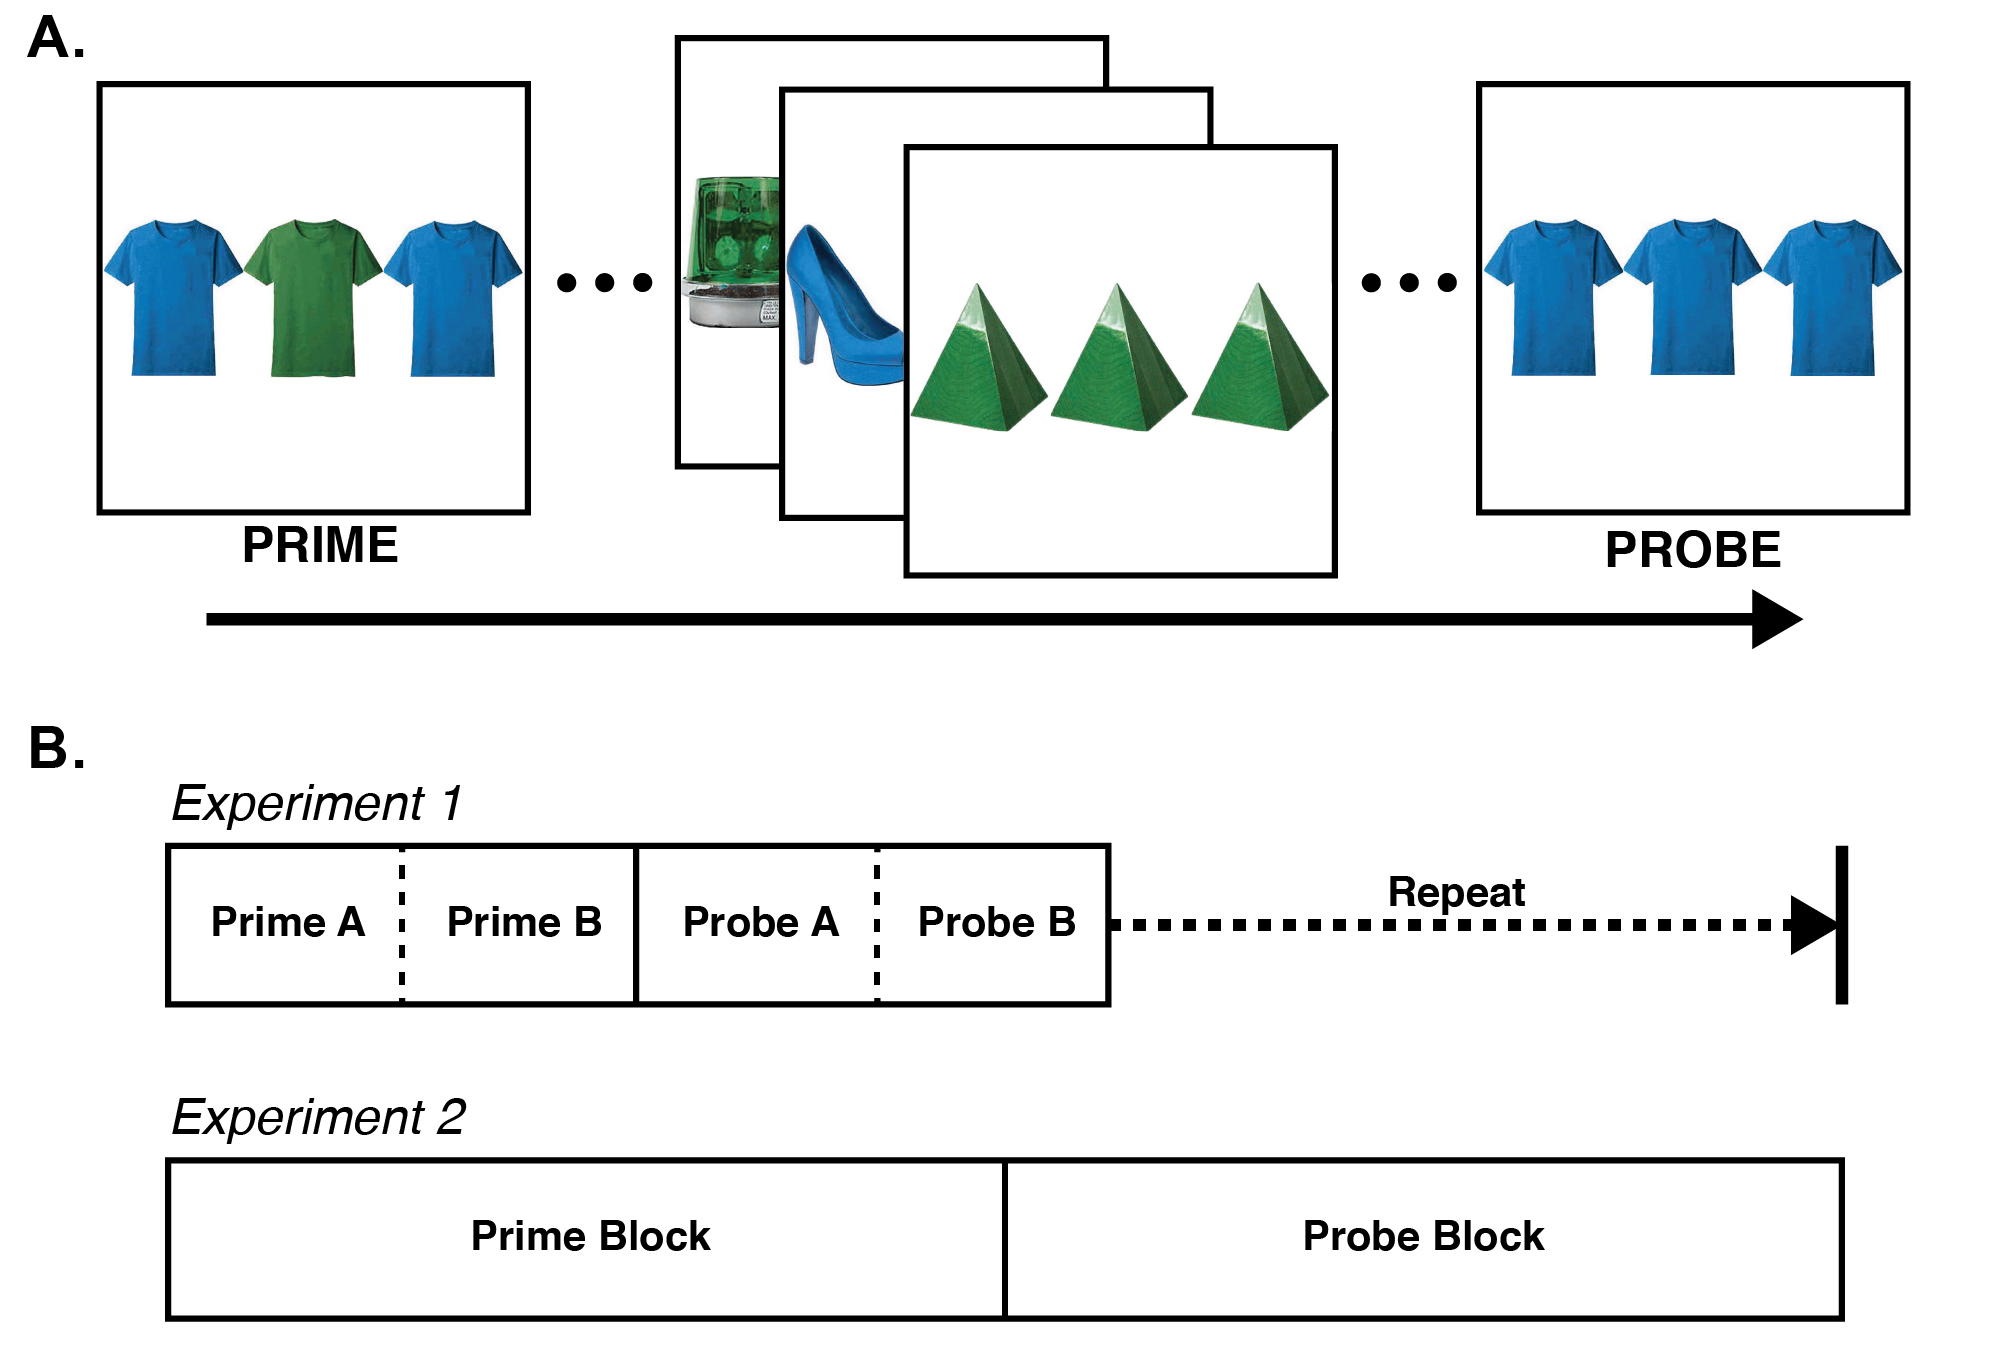
\includegraphics[height=2.75in]{figures/MGfigure1.png}
  \caption{Illustration of the stimuli and prime/probe structure used in all experiments.}
  \caption*{Figure \ref{MG_figure1}A shows examples of the stimuli and basic prime/probe structure used in all experiments. Figure \ref{MG_figure1}B shows the trial block structures from Experiments 1 and 2. In Experiment 1, every block of 16 trials was divided into four sub-blocks, each consisting of four trials (referred to as the Prime A, Prime B, Probe A, and Probe B sub-blocks). The images presented in the Prime A sub-block were then repeated in the Probe A sub-block and images presented in the Prime B sub-block, repeated in the Probe B sub-block. In Experiment 2, there were two blocks of trials, each consisting of 160 trials. The images presented in the Prime block were then repeated in the Probe block.}

  \label{MG_figure1}
\end{figure}

\hypertarget{results-4}{%
\subsection{Results}\label{results-4}}

Participants with mean error rates greater than 20\% were excluded from
the analyses. For experiment 1A, this eliminated five participants, for
1B this eliminated seven participants, and for 1C this eliminated four
participants. For all remaining participants, the RTs from correct
trials in each condition were submitted to an outlier removal procedure
(the non-recursive procedure; Van Selst \& Jolicoeur, 1994) that
eliminated an average of 3.58\%, 3.53\%, and 3.11\% of the observations
from experiments 1A, 1B, and 1C respectively.

\hypertarget{long-term-congruency-sequence-effects.}{%
\subsubsection{Long-term congruency sequence
effects.}\label{long-term-congruency-sequence-effects.}}

The primary question of interest was whether the repetition of unique
stimuli after a single presentation (trial \(n-5\) to \(n-11\)) would
produce sequential-like effects. To address this question, mean RTs from
correct responses on the probe trials and error rates were submitted to
a mixed analysis of variance (ANOVA) with prime congruency (congruent
vs.~incongruent) and probe congruency (congruent vs.~incongruent) as
within-subject factors, and experiment (1A, 1B, and 1C) as the
between-subject factor.

The results of the RT analysis revealed a significant two-way
interaction between prime congruency and probe
congruency,\(F(1, 114) = 10.05\), \(\mathit{MSE} = 1,508.82\),
\(p = .002\), \(\hat{\eta}^2_p = .081\), 90\% CI \([0.02\), \(0.17]\),
demonstrating a smaller congruency effect when the prime stimulus was
incongruent rather than congruent. Furthermore, the three-way
interaction between prime congruency, probe congruency, and experiment,
was non-significant,\(F(2, 114) = 0.11\), \(\mathit{MSE} = 1,508.82\),
\(p = .897\), \(\hat{\eta}^2_p = .002\), 90\% CI \([0\), \(0.01]\),
showing no significant difference between the size or direction of the
long-term sequence effects across experiments.

The results of the error analysis revealed no significant effects of
interest. The three-way interaction between experiment, prime
congruency, and probe congruency was non-significant,
\(F(1, 114) = 1.39\), \(\mathit{MSE} = 11.17\), \(p = .240\),
\(\hat{\eta}^2_p = .012\), 90\% CI \([0\), \(0.06]\), and the two-way
interaction between prime congruency and probe congruency was
non-significant, \(F(2, 114) = 0.48\), \(\mathit{MSE} = 11.17\),
\(p = .621\), \(\hat{\eta}^2_p = .008\), 90\% CI \([0\), \(0.04]\).
Average error rates from experiments 1A, 1B, and 1C (probe trials only),
were 4.38\%, 3.29\%, and 2.9\% respectively.

\hypertarget{congruency-sequence-effects.-1}{%
\subsubsection{\texorpdfstring{\textit{n}-1 congruency sequence
effects.}{-1 congruency sequence effects.}}\label{congruency-sequence-effects.-1}}

In our experimental design, specific stimuli never repeated
trial-to-trial. Another question of interest was whether this design
would still produce \(n-1\) sequence effects when using non-repeating
stimuli. Some previous work has demonstrated that sequence effects were
eliminated when contextual features alternate rather than repeat (Spapé
\& Hommel, 2008) whereas other studies using non-repeating stimuli have
successfully produced sequential effects (Egner, 2010; King, Korb, \&
Egner, 2012). To address this question, mean RTs from correct responses
and error rates were submitted to a mixed analysis of variance (ANOVA)
with trial \(n-1\) congruency (congruent vs.~incongruent) and trial
\(n\) congruency (congruent vs.~incongruent) as within-subject factors,
and experiment (1A, 1B, and 1C) as the between-subject factor (see
\ref{MG_figure2}).

Two results of the RT analysis are of particular interest. First, the
two-way interaction between trial \(n\) congruency and experiment was
significant, \(F(2, 114) = 3.34\), \(\mathit{MSE} = 1,743.37\),
\(p = .039\), \(\hat{\eta}^2_p = .055\), 90\% CI \([0\), \(0.13]\),
suggesting the size of the congruency effect differed across
experiments. Specifically, the congruency effect was smallest in
experiment 1A (M = 33 ms), then experiment 1C (M = 50 ms), and largest
in experiment 1B (M = 60 ms).

Second, the critical two-way interaction between trial \(n-1\)
congruency and trial \(n\) congruency was significant,
\(F(1, 114) = 11.00\), \(\mathit{MSE} = 1,023.99\), \(p = .001\),
\(\hat{\eta}^2_p = .088\), 90\% CI \([0.02\), \(0.18]\) showing a
smaller congruency effect when trial \(n-1\) was incongruent compared to
congruent. However, this interaction was qualified by a significant
three-way interaction between trial \(n-1\) congruency, trial \(n\)
congruency, and experiment, \(F(2, 114) = 3.65\),
\(\mathit{MSE} = 1,023.99\), \(p = .029\), \(\hat{\eta}^2_p = .060\),
90\% CI \([0\), \(0.13]\).

To further probe the three-way interaction, we analyzed each of the
experiments separately. The analysis of experiment 1A resulted in no
significant interaction between trial \(n-1\) congruency and trial \(n\)
congruency, \(F(1, 34) = 0.07\), \(\mathit{MSE} = 1,364.48\),
\(p = .793\), \(\hat{\eta}^2_p = .002\), 90\% CI \([0\), \(0.07]\),
suggesting no sequence effects. However, there were significant two-way
interactions between trial \(n-1\) congruency and trial \(n\) congruency
for both experiment 1B, \(F(1, 31) = 8.56\),
\(\mathit{MSE} = 1,226.60\), \(p = .006\), \(\hat{\eta}^2_p = .216\),
90\% CI \([0.04\), \(0.4]\), and experiment 1C, \(F(1, 49) = 13.87\),
\(\mathit{MSE} = 659.55\), \(p = .001\), \(\hat{\eta}^2_p = .221\), 90\%
CI \([0.07\), \(0.37]\), showing a smaller congruency effect following
incongruent rather than congruent trials.

The results of the error analysis revealed no significant effects of
interest. The three-way interaction between experiment, prime
congruency, and probe congruency was non-significant,
\(F(2, 114) = 0.97\), \(\mathit{MSE} = 7.10\), \(p = .383\),
\(\hat{\eta}^2_p = .017\), 90\% CI \([0\), \(0.06]\), and the two-way
interaction between trial \(n-1\) congruency and trial \(n\) congruency
was non-significant, \(F(1, 114) = 0.91\), \(\mathit{MSE} = 7.10\),
\(p = .341\), \(\hat{\eta}^2_p = .008\), 90\% CI \([0\), \(0.06]\).
Average error rates from experiments 1A, 1B, and 1C, were 3.62\%,
3.18\%, and 2.67\% respectively.

\begin{figure}
  \centering
  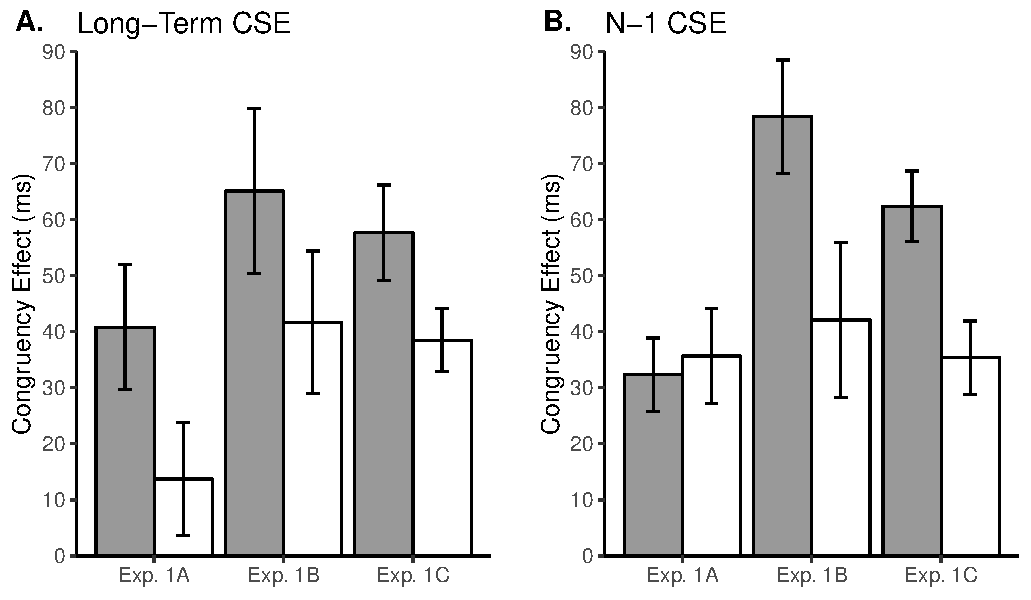
\includegraphics[height=2.75in]{figures/MGfigure2.pdf}
  \caption{Results from Experiment 1}
  \caption*{Figure \ref{MG_figure2}A shows congruency effects in reaction times as a function of Prime Congruency (congruent and incongruent) and Experiment (A, B, and C). Figure \ref{MG_figure2}B shows congruency effects in reaction times as a function of Trial $n-1$ Congruency (congruent and incongruent) and Experiment (A, B, and C). Error bars represent the Standard Error of the Mean (SEM)}

  \label{MG_figure2}
\end{figure}

\hypertarget{discussion-4}{%
\subsection{Discussion}\label{discussion-4}}

Across three replications, we found that a single experience with a
unique stimulus could influence performance 5 to 11 trials after the
initial presentation. Specifically, we consistently found smaller
congruency effects for the probe when the first prime presentation was
incongruent as compared to congruent, demonstrating a long-term
congruency sequence effect. This result is consistent with the
instance-based memory account suggesting that contextual features (image
identity) could cue the rapid adjustment of attentional priorities after
only a single prior presentation.

An unlikely, but alternative interpretation is that the decaying control
signal carried forward over trials from the first presentation to
influence the second. \(n-1\) congruency sequence effects are often
interpreted as the result of control settings or conflict signals from
trial \(n-1\) carrying forward to influence trial n.~Various studies
have shown that sequence effects, given the right conditions, can
persist longer than one trial, from two to four trials (e.g., Jiménez
and Méndez, 2013; Mayr et al., 2003), and up to five seconds (Egner et
al., 2010) after the initial presentation. On the one hand, this
interpretation seems unlikely given the intervening length in our
experiments was much longer than previous demonstrations. On the other
hand, the rate of decay is not well understood, and certainly
conflict-monitoring models are flexible in terms of the speed of decay
(e.g., Botvinick et al., 2001; Braver, 2012). Additionally, there is
evidence that under some conditions the rate of decay could be slowed.
For example, one study demonstrated that the use of proactive strategies
could prevent the sequence effect from decaying as rapidly as previously
demonstrated (Duthoo et al., 2014). It is possible that the use of
contextual cues combined with the frequency and regularity by which they
repeated created some expectation for when contextual cues would repeat.
This may have promoted the use of proactive strategies that slowed the
decay rate long enough to produce our long-term sequence effect.

An additional consideration is whether the secondary task influenced
performance in experiments 1B and 1C. The secondary task had
participants monitor the flanking images and press the spacebar when the
flanking images differed in identity to the target image. The use of
contextual cues in attention tasks is often thought to develop
automatically (e.g., Chun and Jiang, 1998). However, there have been
demonstrations using proportion congruent designs where
context-dependency fails to develop without specific task instructions
to engage in specific strategies (e.g., Brosowsky and Crump, 2016; Crump
et al., 2008). The nature of our secondary task could have caused
participants to attend more to the identities of the images and
encouraged the use of contextual cues. Regardless, the long-term
congruency sequence effect was also found in experiment 1A where
participants did not have the secondary task. So, although it may be
possible that the secondary task contributed to the effects in
experiments 1B and 1C, removing the secondary task was not sufficient
for eliminating the long-term sequence effect.

Finally, experiments 1B and 1C included a secondary task to increase the
amount of conflict, as measured by the congruency effect. Consistent
with that manipulation, we found a smaller congruency effect in
experiment 1A as compared to 1B and 1C. However, the long-term sequence
effect appeared to be insensitive to the conflict manipulation as we
found no significant differences in the size of the long-term sequence
effect across experiments. In contrast, we only found \(n-1\) congruency
sequence effects in experiments 1B and 1C. These findings are consistent
with prior work demonstrating the \(n-1\) sequence effect despite the
use of non-repeating stimuli (Egner et al., 2010; King et al., 2012),
and consistent with prior work showing a sensitivity to the amount of
conflict (Forster et al., 2011; Wendt et al., 2015).

\begin{table}[htpb]
\centering
\caption{Long-Term Congruency Sequence Effects for Experiments 1-3}
\label{MG_table1}
\resizebox{\textwidth}{!}{
\begin{tabular}{rrcccccc}
\toprule & 
& \multicolumn{4}{c}{Probe} & \multicolumn{1}{l}{ Congruency Effect } & \multicolumn{1}{l}{ Long-term CSE} \\
\cmidrule{3-6} &
& \multicolumn{2}{l}{Con} & \multicolumn{2}{l}{Inc} & \multicolumn{1}{l}{ $(I-C)$} & \multicolumn{1}{l}{ ($C_{(I-C)} - I_{(I-C)})$} \\
\cmidrule{3-8}
\multicolumn{2}{c}{Prime} & \multicolumn{1}{l}{RT} & \multicolumn{1}{l}{ER} & \multicolumn{1}{l}{RT} & \multicolumn{1}{l}{ER} & \multicolumn{1}{l}{RT} & \multicolumn{1}{l}{RT} \\
\midrule
\multicolumn{2}{l}{\textbf{Exp. 1A}}  &   &    &     &     &    &  \\
& \multicolumn{1}{l}{Con} & \multicolumn{1}{l}{623 (23)} & \multicolumn{1}{l}{5 (0.8)} & \multicolumn{1}{l}{664 (24)} & \multicolumn{1}{l}{5.12 (0.71)} & \multicolumn{1}{l}{41 (11)} & \multicolumn{1}{l}{27 (13)} \\
& \multicolumn{1}{l}{Inc} & \multicolumn{1}{l}{632 (22)} & \multicolumn{1}{l}{3.69 (0.74)} & \multicolumn{1}{l}{646 (22)} & \multicolumn{1}{l}{3.69 (0.68)} & \multicolumn{1}{l}{14 (10)} & \multicolumn{1}{l}{ }  \\
\multicolumn{2}{l}{\textbf{Exp. 1B}} &    &     &     &     &     &  \\
& \multicolumn{1}{l}{Con} & \multicolumn{1}{l}{766 (22)} & \multicolumn{1}{l}{3.78 (0.71)} & \multicolumn{1}{l}{831 (25)} & \multicolumn{1}{l}{2.21 (0.53)} & \multicolumn{1}{l}{65 (15)} & \multicolumn{1}{l}{23 (16)} \\
& \multicolumn{1}{l}{Inc} & \multicolumn{1}{l}{779 (27)} & \multicolumn{1}{l}{3.65 (0.69)} & \multicolumn{1}{l}{821 (29)} & \multicolumn{1}{l}{3.52 (0.9)} & \multicolumn{1}{l}{42 (13)} & \multicolumn{1}{l}{ }  \\
\multicolumn{2}{l}{\textbf{Exp. 1C}} &    &     &     &     &     &  \\
& \multicolumn{1}{l}{Con} & \multicolumn{1}{l}{774 (26)} & \multicolumn{1}{l}{2.88 (0.44)} & \multicolumn{1}{l}{831 (28)} & \multicolumn{1}{l}{2.21 (0.42)} & \multicolumn{1}{l}{58 (9)} & \multicolumn{1}{l}{19 (9)} \\
& \multicolumn{1}{l}{Inc} & \multicolumn{1}{l}{773 (26)} & \multicolumn{1}{l}{3.12 (0.47)} & \multicolumn{1}{l}{812 (27)} & \multicolumn{1}{l}{3.38 (0.51)} & \multicolumn{1}{l}{38 (6)} & \multicolumn{1}{l}{ }  \\
&       &       &       &       &       &       &  \\
\midrule
\multicolumn{2}{l}{\textbf{Exp. 2A}}  &   &    &     &     &    &  \\
& \multicolumn{1}{l}{Con} & \multicolumn{1}{l}{566 (20)} & \multicolumn{1}{l}{2.99 (0.55)} & \multicolumn{1}{l}{605 (21)} & \multicolumn{1}{l}{4.17 (0.68)} & \multicolumn{1}{l}{39 (6)} & \multicolumn{1}{l}{21 (9)} \\
& \multicolumn{1}{l}{Inc} & \multicolumn{1}{l}{575 (21)} & \multicolumn{1}{l}{2.64 (0.43)} & \multicolumn{1}{l}{593 (19)} & \multicolumn{1}{l}{4.31 (0.55)} & \multicolumn{1}{l}{18 (7)} & \multicolumn{1}{l}{ } \\
\multicolumn{2}{l}{\textbf{Exp. 2B}} &    &     &     &     &     &  \\
& \multicolumn{1}{l}{Con} & \multicolumn{1}{l}{589 (22)} & \multicolumn{1}{l}{1.97 (0.38)} & \multicolumn{1}{l}{647 (21)} & \multicolumn{1}{l}{4.34 (0.66)} & \multicolumn{1}{l}{58 (8)} & \multicolumn{1}{l}{17 (11)} \\
& \multicolumn{1}{l}{Inc} & \multicolumn{1}{l}{589 (23)} & \multicolumn{1}{l}{2.43 (0.38)} & \multicolumn{1}{l}{630 (19)} & \multicolumn{1}{l}{3.95 (0.68)} & \multicolumn{1}{l}{40 (11)} & \multicolumn{1}{l}{ }  \\
&       &       &       &       &       &       &  \\
\midrule
\multicolumn{2}{l}{\textbf{Exp. 3A}}  &   &    &     &     &    &  \\
& \multicolumn{1}{l}{Con} & \multicolumn{1}{l}{842 (21)} & \multicolumn{1}{l}{2.37 (0.5)} & \multicolumn{1}{l}{880 (22)} & \multicolumn{1}{l}{3.03 (0.63)} & \multicolumn{1}{l}{38 (8)} & \multicolumn{1}{l}{13 (14)}  \\
& \multicolumn{1}{l}{Inc} & \multicolumn{1}{l}{846 (24)} & \multicolumn{1}{l}{2.84 (0.55)} & \multicolumn{1}{l}{871 (21)} & \multicolumn{1}{l}{2.94 (0.57)} & \multicolumn{1}{l}{25 (11)} & \multicolumn{1}{l}{ }  \\
\multicolumn{2}{l}{\textbf{Exp. 3B}} &    &     &     &     &     &  \\
& \multicolumn{1}{l}{Con} & \multicolumn{1}{l}{837 (22)} & \multicolumn{1}{l}{2.73 (0.45)} & \multicolumn{1}{l}{867 (20)} & \multicolumn{1}{l}{2.5 (0.48)} & \multicolumn{1}{l}{30 (7)} & \multicolumn{1}{l}{0 (10)} \\
& \multicolumn{1}{l}{Inc} & \multicolumn{1}{l}{840 (22)} & \multicolumn{1}{l}{1.92 (0.39)} & \multicolumn{1}{l}{870 (23)} & \multicolumn{1}{l}{2.15 (0.47)} & \multicolumn{1}{l}{30 (7)} & \multicolumn{1}{l}{ }  \\
&       &       &       &       &       &       &  \\
\bottomrule
\multicolumn{8}{l}{\textit{Note}: RT = Reaction Time (ms);  ER = Error Rates (\%);  } \\
\multicolumn{8}{l}{Con/C  congruent; Inc/I  incongruent; standard errors are presented in parentheses.} \\
\end{tabular}
}%
\end{table}

\begin{table}[htpb]
\centering
\caption{$\textit{N}-1$ Congruency Sequence Effects for Experiments 1-3}
\label{MG_table2}
\resizebox{\textwidth}{!}{
\begin{tabular}{rrcccccc}
\toprule & 
& \multicolumn{4}{c}{Trial $\textit{n}$} & \multicolumn{1}{l}{Congruency Effect } & \multicolumn{1}{l}{$\textit{N}-1$ CSE} \\
\cmidrule{3-6} &
& \multicolumn{2}{l}{Con} & \multicolumn{2}{l}{ Inc} & \multicolumn{1}{l}{ $(I-C)$} & \multicolumn{1}{l}{ ($C_{(I-C)} - I_{(I-C)})$} \\
\cmidrule{3-8}
\multicolumn{2}{c}{Trial \textit{n}-1} & \multicolumn{1}{l}{RT} & \multicolumn{1}{l}{ER} & \multicolumn{1}{l}{RT} & \multicolumn{1}{l}{ER} & \multicolumn{1}{l}{RT} & \multicolumn{1}{l}{RT} \\
\midrule
\multicolumn{2}{l}{\textbf{Exp. 1A}}  &   &    &     &     &    &  \\
& \multicolumn{1}{l}{Con} & \multicolumn{1}{l}{626 (22)} & \multicolumn{1}{l}{2.97 (0.55)} & \multicolumn{1}{l}{658 (22)} & \multicolumn{1}{l}{3.48 (0.48)} & \multicolumn{1}{l}{32 (7)} & \multicolumn{1}{l}{-3 (12)} \\
& \multicolumn{1}{l}{Inc} & \multicolumn{1}{l}{635 (21)} & \multicolumn{1}{l}{3.55 (0.46)} & \multicolumn{1}{l}{671 (25)} & \multicolumn{1}{l}{4.48 (0.71)} & \multicolumn{1}{l}{36 (8)} & \multicolumn{1}{l}{ } \\
\multicolumn{2}{l}{\textbf{Exp. 1B}} &    &     &     &     &     &  \\
& \multicolumn{1}{l}{Con} & \multicolumn{1}{l}{753 (21)} & \multicolumn{1}{l}{2.4 (0.51)} & \multicolumn{1}{l}{832 (25)} & \multicolumn{1}{l}{3.48 (0.53)} & \multicolumn{1}{l}{78 (10)} & \multicolumn{1}{l}{36 (12)} \\
& \multicolumn{1}{l}{Inc} & \multicolumn{1}{l}{791 (24)} & \multicolumn{1}{l}{3.58 (0.54)} & \multicolumn{1}{l}{833 (25)} & \multicolumn{1}{l}{3.27 (0.71)} & \multicolumn{1}{l}{42 (14)} & \multicolumn{1}{l}{ } \\
\multicolumn{2}{l}{\textbf{Exp. 1C}} &    &     &     &     &     &  \\
& \multicolumn{1}{l}{Con} & \multicolumn{1}{l}{771 (27)} & \multicolumn{1}{l}{2.46 (0.37)} & \multicolumn{1}{l}{834 (27)} & \multicolumn{1}{l}{2.66 (0.39)} & \multicolumn{1}{l}{62 (6)} & \multicolumn{1}{l}{27 (7)} \\
& \multicolumn{1}{l}{Inc} & \multicolumn{1}{l}{794 (25)} & \multicolumn{1}{l}{2.91 (0.4)} & \multicolumn{1}{l}{829 (26)} & \multicolumn{1}{l}{2.65 (0.37)} & \multicolumn{1}{l}{35 (7)} & \multicolumn{1}{l}{ } \\
&       &       &       &       &       &       &  \\
\midrule
\multicolumn{2}{l}{\textbf{Exp. 2A}}  &   &    &     &     &    &  \\
& \multicolumn{1}{l}{Con} & \multicolumn{1}{l}{557 (17)} & \multicolumn{1}{l}{2.36 (0.38)} & \multicolumn{1}{l}{593 (16)} & \multicolumn{1}{l}{4.36 (0.57)} & \multicolumn{1}{l}{36 (6)} & \multicolumn{1}{l}{8 (8)} \\
& \multicolumn{1}{l}{Inc} & \multicolumn{1}{l}{576 (18)} & \multicolumn{1}{l}{3.59 (0.46)} & \multicolumn{1}{l}{605 (19)} & \multicolumn{1}{l}{3.8 (0.6)} & \multicolumn{1}{l}{28 (6)} & \multicolumn{1}{l}{ } \\
\multicolumn{2}{l}{\textbf{Exp. 2B}} &    &     &     &     &     &  \\
& \multicolumn{1}{l}{Con} & \multicolumn{1}{l}{568 (20)} & \multicolumn{1}{l}{1.91 (0.34)} & \multicolumn{1}{l}{638 (20)} & \multicolumn{1}{l}{4.67 (0.61)} & \multicolumn{1}{l}{70 (5)} & \multicolumn{1}{l}{33 (6)} \\
& \multicolumn{1}{l}{Inc} & \multicolumn{1}{l}{606 (24)} & \multicolumn{1}{l}{2.83 (0.41)} & \multicolumn{1}{l}{643 (23)} & \multicolumn{1}{l}{3.78 (0.58)} & \multicolumn{1}{l}{37 (7)} & \multicolumn{1}{l}{ } \\
&       &       &       &       &       &       &  \\
\midrule
\multicolumn{2}{l}{\textbf{Exp. 3A}}  &   &    &     &     &    &  \\
& \multicolumn{1}{l}{Con} & \multicolumn{1}{l}{837 (24)} & \multicolumn{1}{l}{2.18 (0.44)} & \multicolumn{1}{l}{879 (21)} & \multicolumn{1}{l}{2.65 (0.41)} & \multicolumn{1}{l}{43 (8)} & \multicolumn{1}{l}{22 (12)} \\
& \multicolumn{1}{l}{Inc} & \multicolumn{1}{l}{855 (21)} & \multicolumn{1}{l}{2.83 (0.4)} & \multicolumn{1}{l}{876 (22)} & \multicolumn{1}{l}{2.85 (0.56)} & \multicolumn{1}{l}{20 (8)} & \multicolumn{1}{l}{ } \\
\multicolumn{2}{l}{\textbf{Exp. 3B}} &    &     &     &     &     &  \\
& \multicolumn{1}{l}{Con} & \multicolumn{1}{l}{860 (23)} & \multicolumn{1}{l}{2.54 (0.38)} & \multicolumn{1}{l}{889 (24)} & \multicolumn{1}{l}{2.38 (0.42)} & \multicolumn{1}{l}{30 (7)} & \multicolumn{1}{l}{13 (10)} \\
& \multicolumn{1}{l}{Inc} & \multicolumn{1}{l}{873 (24)} & \multicolumn{1}{l}{2.28 (0.36)} & \multicolumn{1}{l}{889 (23)} & \multicolumn{1}{l}{2.43 (0.35)} & \multicolumn{1}{l}{16 (8)} & \multicolumn{1}{l}{ } \\
&       &       &       &       &       &       &  \\
\bottomrule
\multicolumn{8}{l}{\textit{Note}: RT = Reaction Time (ms);  ER = Error Rates (\%);  } \\
\multicolumn{8}{l}{Con/C  congruent; Inc/I  incongruent; standard errors are presented in parentheses.} \\
\end{tabular}
}%
\end{table}

\hypertarget{experiment-2a-and-2b}{%
\section{Experiment 2A and 2B}\label{experiment-2a-and-2b}}

In experiment one, across three replications, we found long-term
congruency sequence effects when there were 5 to 11 intervening trials
between the first and second presentation of a unique stimulus. The
goals of experiment two were to conceptually replicate and extend the
findings from experiment one by increasing the number of intervening
trials between the prime and probe pairs, increasing the variability in
the frequency of stimulus repetition, and including an alternate
conflict manipulation.

For both experiments 2A and 2B, the primary task was the same as
experiment one which involved identifying the color of a central image
(either blue or green) flanked on the left and right by the same image
presented in either the same (congruent) or the alternate color
(incongruent). Each image was only presented once as a prime stimulus,
and once as a probe stimulus. Importantly, the experiment consisted of
two blocks of 160 trials; A prime block followed by a probe block. Each
block was randomized such that the distance between any given prime and
probe stimulus ranged from 1 to 319 trials (160 trials, on average). To
increase conflict in experiment 2B, the flanking images preceded the
target image by 100 ms, a manipulation known to increase the congruency
effect (Wendt et al., 2015).

\hypertarget{methods-5}{%
\subsection{Methods}\label{methods-5}}

\hypertarget{participants.-1}{%
\subsubsection{Participants.}\label{participants.-1}}

All participants were recruited from Amazon Mechanical Turk (AMT) and
compensated \$2.00 for participating. The amount compensated was
calculated by estimating the maximum amount of time required to complete
each experiment and multiplying by \$6.00 per hour. For each experiment
the number of HITs (Human intelligence tasks, an Amazon term for a
work-unit) refers to the number of participants who initiated the study
and each experiment consisted of unique participants. Participants were
included in the study if they completed all trials. For experiment 2A,
40 HITs were posted, and 39 participants completed all trials. For
experiment 2B, 40 HITs were posted, and 40 participants completed all
trials.

\hypertarget{apparatus-stimuli.-1}{%
\subsubsection{Apparatus \& Stimuli.}\label{apparatus-stimuli.-1}}

The apparatus and stimuli were identical to those used in experiment 1.
Design. Experiment 2 used a 2x2x2 mixed design with prime congruency
(congruent vs.~incongruent) and probe congruency (congruent
vs.~incongruent) as within-subject factors, and experiment (2A and 2B)
as the between-subject factor.

Experiments 2A and 2B were both constructed using the same general
method. Both experiments consisted of 320 total trials divided into two
halves, a prime block and probe block. The prime block was constructed
using 160 unique images randomly selected for each participant from the
total 540 images (Brady et al., 2013). The images presented in the prime
block were then repeated in the probe block. The trial order for each
block was randomized, so the distance between any given probe (trial n)
and prime stimulus paired ranged from \(n-1\) to \(n-319\). Each
experiment consisted of 50\% congruent/incongruent trials, an equal
number of each congruency combination between prime/probe pairs (i.e.,
Con - Con, Con - Inc, Inc - Inc, and Inc - Con), and an equal number of
response repetition and response alternation prime/probe pairs.

\hypertarget{procedure.-1}{%
\subsubsection{Procedure.}\label{procedure.-1}}

All participants were AMT workers who found the experiment using the AMT
system. The participant recruitment procedure and tasks were approved by
the Brooklyn College Institutional Review Board. Each participant read a
short description of the task and gave consent by pressing a button
acknowledging they had read the displayed consent form. Participants
then completed a short demographic survey, and proceeded to the main
task, which was displayed as a pop-up window. Participants were
instructed to identify the color of the center image on each trial as
quickly and accurately as possible by pressing `g' if the image was
green, and `b' if the image was blue. Throughout the course of the
experiment the upper left corner of the display indicated the number of
completed and remaining trials, as well as an instruction reminder
button that displayed the instructions in a new pop-up window.

For experiment 2A, each trial began with a fixation cross presented in
the center of the screen for 1,000 ms, followed by a blank ISI of 250
ms. Next, the flanker stimulus appeared in the center of screen, and
remained on screen until a response was made. Feedback indicating
whether the answer was correct or incorrect was presented above the
target stimulus following a response and remained on-screen for 500 ms
which automatically triggered the next trial. For experiment 2B, each
trial began with a fixation cross presented in the center of the screen
for 1,000 ms, followed by a blank ISI of 250 ms. Next, the flanking
images appeared for 100 ms followed by the presentation of the center
image. All images remained on screen until a response was given.
Feedback indicating whether the answer was correct or incorrect was
presented above the target stimulus following a response and remained
on-screen for 500 ms which automatically triggered the next trial. In
both experiments, after every 80 trials, a message appeared on-screen
that instructed participants to take a short break and to press the
button when they were ready to continue.

\hypertarget{results-5}{%
\subsection{Results}\label{results-5}}

Participants with mean error rates greater than 20\% were excluded from
the analyses. For experiment 2A, this eliminated three participants and
for 2B this eliminated two participants. For all remaining participants,
the RTs from correct trials in each condition were submitted to an
outlier removal procedure (the non-recursive procedure; Van Selst \&
Jolicoeur, 1994) that eliminated an average of 3.2\% and 3.3\% of the
observations from experiments 2A and 2B, respectively.

\hypertarget{long-term-congruency-sequence-effects.-1}{%
\subsubsection{Long-term congruency sequence
effects.}\label{long-term-congruency-sequence-effects.-1}}

Mean RTs from correct responses on probe trials and error rates were
submitted to a mixed analysis of variance (ANOVA) with prime congruency
(congruent vs.~incongruent) and probe congruency (congruent
vs.~incongruent) as within-subject factors, and experiment (2A and 2B)
as the between-subject factor (see Figure \ref{MG_figure3}).

The results of the RT analysis revealed a significant two-way
interaction between prime congruency and probe congruency,
\(F(1, 72) = 6.99\), \(\mathit{MSE} = 980.13\), \(p = .010\),
\(\hat{\eta}^2_p = .089\), 90\% CI \([0.01\), \(0.2]\), demonstrating a
smaller congruency effect when the prime stimulus was incongruent rather
than congruent. Additionally, the three-way interaction between prime
congruency, probe congruency, and experiment, was non-significant,
\(F(1, 72) = 0.09\), \(\mathit{MSE} = 980.13\), \(p = .768\),
\(\hat{\eta}^2_p = .001\), 90\% CI \([0\), \(0.04]\), showing no
difference between the size or direction of the long-term sequence
effects across experiments.

The results of the error analysis revealed no significant effects of
interest. The three-way interaction between experiment, prime
congruency, and probe congruency was
non-significant,\(F(1, 72) = 1.23\), \(\mathit{MSE} = 6.77\),
\(p = .272\), \(\hat{\eta}^2_p = .017\), 90\% CI \([0\), \(0.09]\), and
the two-way interaction between prime congruency and probe congruency
was non-significant, \(F(1, 72) = 0.09\), \(\mathit{MSE} = 6.77\),
\(p = .761\), \(\hat{\eta}^2_p = .001\), 90\% CI \([0\), \(0.04]\).
Average error rates from experiments 2A and 2C (probe trials only), were
3.52\% and 3.17\% respectively.

\hypertarget{congruency-sequence-effects.-2}{%
\subsubsection{\texorpdfstring{\textit{n}-1 congruency sequence
effects.}{-1 congruency sequence effects.}}\label{congruency-sequence-effects.-2}}

Mean RTs from correct responses and mean error rates were submitted to a
mixed analysis of variance (ANOVA) with trial \(n-1\) congruency
(congruent vs.~incongruent) and trial \(n\) congruency (congruent
vs.~incongruent) as within-subject factors, and experiment (2A and 2B)
as the between-subject factor (see Figure \ref{MG_figure3}).

The RT analysis resulted in a significant two-way interaction between
trial \(n\) congruency and experiment, \(F(1, 72) = 9.90\),
\(\mathit{MSE} = 851.61\), \(p = .002\), \(\hat{\eta}^2_p = .121\), 90\%
CI \([0.03\), \(0.24]\); The size of the congruency effect was
significantly smaller in experiment 2A (M = 33 ms), as compared to
experiment 2B (M = 54 ms).

The critical two-way interaction between trial \(n-1\) congruency and
trial \(n\) congruency was also significant, \(F(1, 72) = 15.92\),
\(\mathit{MSE} = 481.26\), \(p < .001\), \(\hat{\eta}^2_p = .181\), 90\%
CI \([0.06\), \(0.31]\), demonstrating a smaller congruency effect when
trial \(n-1\) was incongruent rather than congruent. However, this was
qualified by a three-way interaction between trial \(n-1\) congruency,
trial \(n\) congruency, and experiment, \(F(1, 72) = 5.99\),
\(\mathit{MSE} = 481.26\), \(p = .017\), \(\hat{\eta}^2_p = .077\), 90\%
CI \([0.01\), \(0.19]\).

A separate analysis of experiment 2A showed no significant interaction
between trial \(n-1\) congruency and trial \(n\) congruency,
\(F(1, 35) = 0.91\), \(\mathit{MSE} = 614.66\), \(p = .347\),
\(\hat{\eta}^2_p = .025\), 90\% CI \([0\), \(0.15]\). However, the
analysis of experiment 2B showed a significant two-way interaction,
\(F(1, 37) = 28.87\), \(\mathit{MSE} = 355.08\), \(p < .001\),
\(\hat{\eta}^2_p = .438\), 90\% CI \([0.23\), \(0.58]\), with a smaller
congruency effect when trial \(n-1\) was incongruent rather than
congruent.

The results of the error analysis revealed a significant two-way
interaction between trial \(n-1\) congruency and trial \(n\)
congruency,\(F(1, 72) = 13.69\), \(\mathit{MSE} = 4.35\), \(p < .001\),
\(\hat{\eta}^2_p = .160\), 90\% CI \([0.05\), \(0.28]\), showing a
larger congruency effect following a congruent (M = 2.37\%), as compared
to an incongruent trial (M = 0.57\%). However, the three-way interaction
between experiment, trial \(n-1\) congruency, and trial \(n\) congruency
was non-significant, \(F(1, 72) < 0.01\), \(\mathit{MSE} = 4.35\),
\(p = .978\), \(\hat{\eta}^2_p < .001\), 90\% CI \([0\), \(1]\). Average
error rates from experiments 2A and 2C, were 3.53\% and 3.3\%
respectively.

\begin{figure}
  \centering
  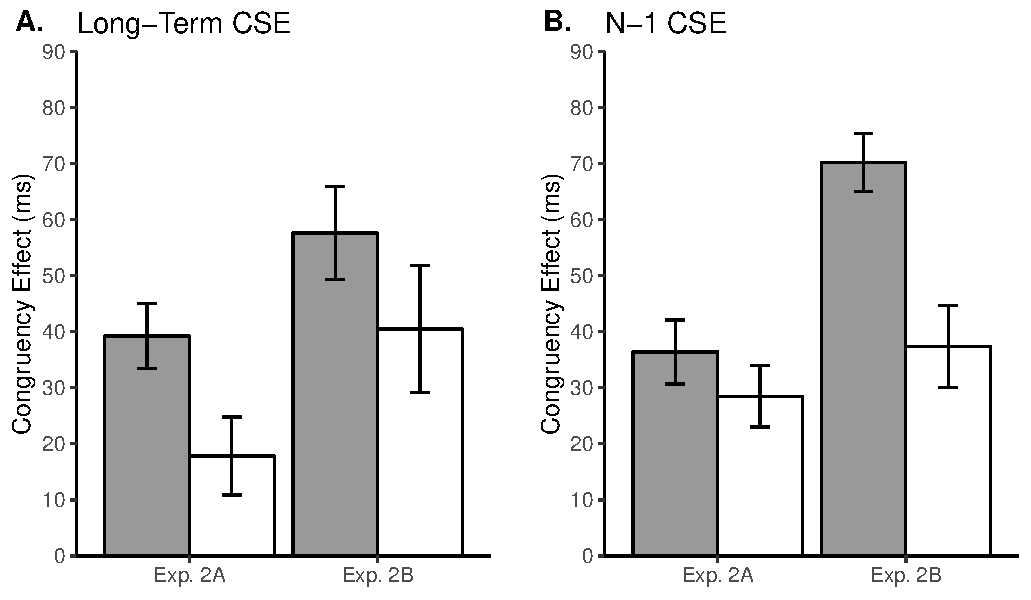
\includegraphics[height=2.75in]{figures/MGfigure3.pdf}
  \caption{Results from Experiment 2}
  \caption*{Figure \ref{MG_figure3}A shows congruency effects in reaction times as a function of Prime Congruency (congruent and incongruent) and Experiment (A and B). Figure \ref{MG_figure3}B shows congruency effects in reaction times as a function of Trial $n-1$ Congruency (congruent and incongruent) and Experiment (A and B). Error bars represent the Standard Error of the Mean (SEM).}

  \label{MG_figure3}
\end{figure}

\hypertarget{discussion-5}{%
\subsection{Discussion}\label{discussion-5}}

The critical result in experiment two was that congruency effects were
significantly smaller on probe trials paired with an incongruent as
compared to congruent prime trial. Experiment 2 therefore conceptually
replicates experiment 1 and demonstrates long-term congruency sequence
effects with 1 to 319 intervening trials, increased variability in the
frequency of stimulus repetition, and an alternate conflict
manipulation.

Additionally, the level of conflict was manipulated across experiments.
Consistent with our manipulation, the congruency effect was
significantly larger in experiment 2B as compared to 2A. However, this
manipulation did not modulate the size or direction of the long-term
congruency sequence effect. In contrast, we only found \(n-1\)
congruency sequence effects in experiment 2B, suggesting a sensitivity
to the level of conflict, and replicating the results of experiment 1.

\hypertarget{experiment-3a-and-3b}{%
\section{Experiment 3A and 3B}\label{experiment-3a-and-3b}}

Across experiments 1 and 2, we have demonstrated long-term congruency
sequence effects with as many as 160 intervening trials between the
first and second presentation of a unique stimulus. However, both
experiments used a 2-choice flanker task resulting in some
feature-overlap between the prime and probe trial. Feature integration
accounts have proposed that differences in match between features
presented on trial \(n-1\) and trial \(n\) could account for congruency
sequence effects by way of event files and a memory retrieval process
(Hommel, 1998; Hommel et al., 2001, 2004). This issue will be discussed
in greater detail in the general discussion, however, the goal of
experiment 3 was to test whether the long-term congruency effect would
persist when the prime and probe trials consist entirely of
non-overlapping color features.

For both experiments 3A and 3B, the primary task was the same as
experiments 1 and 2 identifying the color of a central image flanked on
the left and right by the same image presented in either the same
(congruent) or the alternate color (incongruent). Each image was only
presented once as a prime stimulus, and once as a probe stimulus.
However, in contrast to experiments 1 and 2, images could appear in one
of four colors (red, blue, green, or yellow). For each participant,
colors were randomly assigned to two mutually exclusive color sets. Each
prime/probe stimulus pair used both color sets ensuring that colors did
not overlap between the prime and probe trial.

Except for the image colors, experiment 3A followed the same methods as
experiment 1A such that the distance between any given prime and probe
stimulus ranged from 5 to 11 trials (8 trials, on average). Similarly,
experiment 3B followed the same methods as experiment 2A such that the
distance between any given prime and probe stimulus ranged from 1 to 319
(160 trials, on average).

\hypertarget{methods-6}{%
\subsection{Methods}\label{methods-6}}

\hypertarget{participants.-2}{%
\subsubsection{Participants.}\label{participants.-2}}

All participants were recruited from Amazon Mechanical Turk (AMT) and
compensated \$1.00 for participating. The amount compensated was
calculated by estimating the maximum amount of time required to complete
each experiment and multiplying by \$6.00 per hour. For each experiment
the number of HITs (Human intelligence tasks, an Amazon term for a
work-unit) refers to the number of participants who initiated the study
and each experiment consisted of unique participants. Participants were
included in the study if they completed all trials. For experiment 3A,
50 HITs were posted, and 50 participants completed all trials. For
experiment 3B, 50 HITs were posted, and 47 participants completed all
trials.

\hypertarget{apparatus-stimuli.-2}{%
\subsubsection{Apparatus \& Stimuli.}\label{apparatus-stimuli.-2}}

The apparatus and stimuli were identical to those used in experiments 1
and 2.

\hypertarget{design.-1}{%
\subsubsection{Design.}\label{design.-1}}

Experiment 3 used a 2x2 within-subjects design with prime congruency
(congruent vs.~incongruent) and probe congruency (congruent
vs.~incongruent) as factors.

Experiment 3A was constructed using the methods as described in
experiment 1A. Therefore, experiment 3A consisted of 192 total trials
with the distance between each prime and probe stimulus pair ranging
from \(n-5\) to \(n-11\). Experiment 3B was constructed using the
methods as described in experiment 2. Therefore, experiment 3B consisted
of 320 total trials with the distance between each prime and probe
stimulus pair ranged from \(n-1\) to \(n-319\). Each experiment
consisted of 50\% congruent/incongruent trials, an equal number of each
congruency combination between prime/probe pairs (i.e., Con - Con, Con -
Inc, Inc - Inc, and Inc - Con). Images were randomly selected for every
participant from the total 540 images (Brady et al., 2013) and randomly
assigned a color and condition. Each image was only presented twice
during the experiment: once in a prime block and once in a probe block.

The colors of the images however, differed from experiments 1 and 2. For
experiment 3, images could appear in one of four colors: blue, green,
red, or yellow. For each participant, the four colors were randomly
assigned to two color sets (e.g., blue/green, red/yellow), such that
colors in differing sets were never presented together on a single trial
(e.g., green/yellow never appeared together). Additionally, each
prime/probe pair always consisted of colors from both sets to ensure
that colors did not repeat from the prime to probe trial. The assignment
of colors to prime/probe trials was counterbalanced for each
participant. Therefore, on 50\% of trials, color set 1 was assigned to
the prime stimuli and color set 2 to the corresponding probe, and on the
other half, color set 2 was assigned to the prime and color set 1 to the
probe.

\hypertarget{procedure.-2}{%
\subsubsection{Procedure.}\label{procedure.-2}}

The procedure was identical to experiments 1 and 2. However, because of
the use of four colors, participants were instructed to identify the
color of the center image on each trial as quickly and accurately as
possible by pressing `b' if the image was blue, `g' if the image was
green, `r' if the image was red, and `y' if the image was yellow.

\hypertarget{results-6}{%
\subsection{Results}\label{results-6}}

Participants with mean error rates greater than 20\% were excluded from
the analyses. For experiment 3A, this eliminated six participants and
for 3B this eliminated four participants. For all remaining
participants, the RTs from correct trials in each condition were
submitted to an outlier removal procedure (the non-recursive procedure;
Van Selst \& Jolicoeur, 1994) that eliminated an average of 3.19\% and
2.89\% of the observations from experiments 3A and 3B, respectively.

\hypertarget{experiment-3a--8-trials}{%
\subsection{\texorpdfstring{Experiment 3A: \textit{n}-8
trials}{Experiment 3A: -8 trials}}\label{experiment-3a--8-trials}}

\hypertarget{long-term-congruency-sequence-effects.-2}{%
\subsubsection{Long-term congruency sequence
effects.}\label{long-term-congruency-sequence-effects.-2}}

Mean RTs from correct responses and error rates were submitted to a
repeated measures analysis of variance (ANOVA) with prime congruency
(congruent vs.~incongruent) and probe congruency (congruent
vs.~incongruent) as factors. As a result, the two-way interaction
between prime congruency and probe congruency was non-significant,
\(F(1, 43) = 0.84\), \(\mathit{MSE} = 2,173.47\), \(p = .365\),
\(\hat{\eta}^2_p = .019\), 90\% CI \([0\), \(0.13]\), showing no
differences between the congruency effects when the prime was congruent
versus incongruent.

The results of the error analysis also revealed no significant effects
of interest. The two-way interaction between prime congruency and probe
congruency was non-significant, \(F(1, 43) = 0.36\),
\(\mathit{MSE} = 9.81\), \(p = .551\), \(\hat{\eta}^2_p = .008\), 90\%
CI \([0\), \(0.1]\).

\hypertarget{congruency-sequence-effects.-3}{%
\subsubsection{\texorpdfstring{\textit{n}-1 congruency sequence
effects.}{-1 congruency sequence effects.}}\label{congruency-sequence-effects.-3}}

Mean RTs from correct responses and mean error rates were submitted to a
repeated measures analysis of variance (ANOVA) with trial \(n-1\)
congruency (congruent vs.~incongruent) and trial \(n\) congruency
(congruent vs.~incongruent) as within-subject factors. As a result, the
two-way interaction between trial \(n-1\) and trial \(n\) congruency was
marginal, though non-significant, \(F(1, 43) = 3.57\),
\(\mathit{MSE} = 1,546.60\), \(p = .066\), \(\hat{\eta}^2_p = .077\),
90\% CI \([0\), \(0.22]\), showing no differences between the congruency
effects when trial \(n-1\) was congruent versus incongruent.

The results of the error analysis also revealed no significant effects
of interest. The two-way interaction between trial \(n-1\) congruency
and trial \(n\) congruency was non-significant, \(F(1, 43) = 0.46\),
\(\mathit{MSE} = 4.80\), \(p = .503\), \(\hat{\eta}^2_p = .011\), 90\%
CI \([0\), \(0.11]\). Average error rates were 2.36\%.

\hypertarget{experiment-3b--160-trials}{%
\subsection{\texorpdfstring{Experiment 3B: \textit{n}-160
trials}{Experiment 3B: -160 trials}}\label{experiment-3b--160-trials}}

\hypertarget{long-term-congruency-sequence-effects.-3}{%
\subsubsection{Long-term congruency sequence
effects.}\label{long-term-congruency-sequence-effects.-3}}

Mean RTs from correct responses and mean error rates from probe trials
were submitted to a repeated measures analysis of variance (ANOVA) with
prime congruency (congruent vs.~incongruent) and probe congruency
(congruent vs.~incongruent) as factors (see Figure \ref{MG_figure4}). As
a result, the two-way interaction between prime congruency and probe
congruency was non-significant, \(F(1, 42) < 0.01\),
\(\mathit{MSE} = 973.11\), \(p = .961\), \(\hat{\eta}^2_p < .001\), 90\%
CI \([0\), \(1]\), showing no differences between the congruency effects
when the prime was congruent versus incongruent.

The results of the error analysis also revealed no significant effects
of interest. The two-way interaction between prime congruency and probe
congruency was non-significant, \(F(1, 42) = 0.27\),
\(\mathit{MSE} = 8.50\), \(p = .604\), \(\hat{\eta}^2_p = .006\), 90\%
CI \([0\), \(0.09]\).

\hypertarget{congruency-sequence-effects.-4}{%
\subsubsection{\texorpdfstring{\textit{n}-1 congruency sequence
effects.}{-1 congruency sequence effects.}}\label{congruency-sequence-effects.-4}}

Mean RTs from correct responses and mean error rates were submitted to a
repeated measures analysis of variance (ANOVA) with trial \(n-1\)
congruency (congruent vs.~incongruent) and trial \(n\) congruency
(congruent vs.~incongruent) as within-subject factors. As a result, the
two-way interaction between trial \(n-1\) and trial \(n\) congruency was
non-significant,\(F(1, 42) = 1.58\), \(\mathit{MSE} = 1,178.33\),
\(p = .215\), \(\hat{\eta}^2_p = .036\), 90\% CI \([0\), \(0.16]\),
showing no differences between the congruency effects when trial \(n-1\)
was congruent versus incongruent.

Similarly, the results of the error analysis also revealed no
significant effects of interest. The two-way interaction between trial
\(n-1\) congruency and trial \(n\) congruency was
non-significant,\(F(1, 42) = 0.23\), \(\mathit{MSE} = 4.51\),
\(p = .636\), \(\hat{\eta}^2_p = .005\), 90\% CI \([0\), \(0.09]\).
Average error rates were 2.58\%.

\begin{figure}
  \centering
  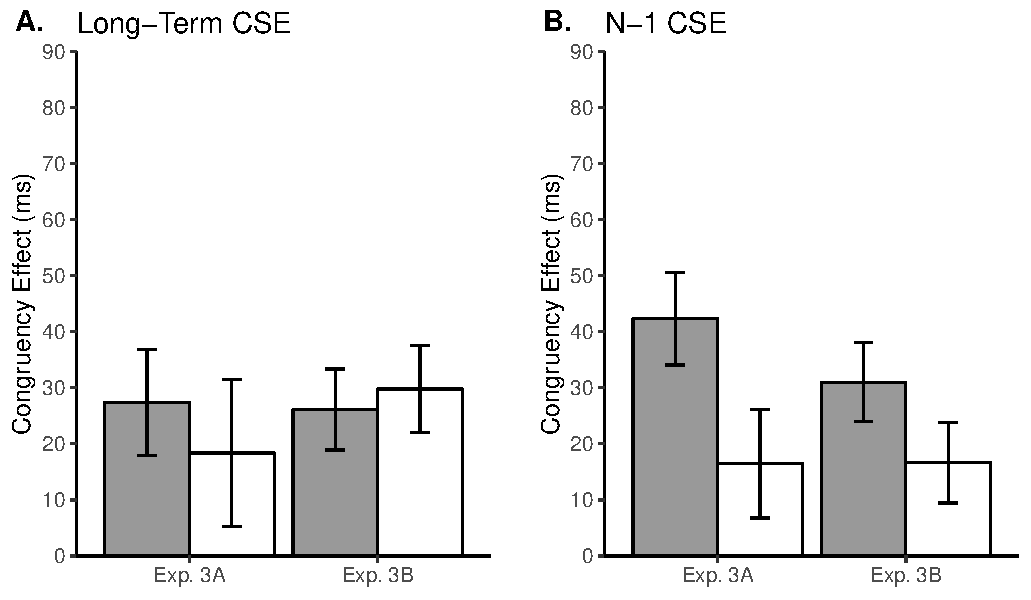
\includegraphics[height=2.75in]{figures/MGfigure4.pdf}
  \caption{Results from Experiment 3}
  \caption*{Figure \ref{MG_figure4}A shows congruency effects in reaction times as a function of Prime Congruency (congruent and incongruent) and Experiment (A and B). Figure \ref{MG_figure4}B shows congruency effects in reaction times as a function of Trial $n-1$ Congruency (congruent and incongruent) and Experiment (A and B). Error bars represent the Standard Error of the Mean (SEM). In both experiments, the interaction was non-significant ($p > .05$).}

  \label{MG_figure4}
\end{figure}

\hypertarget{discussion-6}{%
\subsection{Discussion}\label{discussion-6}}

The critical result of experiment three was the failure to find
long-term congruency sequence effects. Experiment 3, therefore failed to
replicate experiments 1 and 2 when color features did not overlap
between prime and probe stimuli. A positive finding would have
convincingly ruled out a potential long-term feature integration account
of the findings from experiments 1 and 2. However, the failure to find
the effect is more ambiguous. Any theory that relies on memory-retrieval
might make the prediction that decreasing the similarity between the
prime and probe could diminish or eliminate the effect because the probe
is no longer an adequate retrieval cue. Therefore, the finding in
experiment 3 does not provide direct evidence for a long-term feature
integration account though it does fail to rule out such a possibility.
These issues are discussed in greater detail in the general discussion.

\hypertarget{stimulus-response-repetition-analyses}{%
\section{Stimulus-Response Repetition
Analyses}\label{stimulus-response-repetition-analyses}}

Previous work has demonstrated that stimulus-response repetition biases
confounded with congruency manipulations may contribute to, or account
entirely for, sequential modulations of congruency effects (e.g., Mayr
et al., 2003). This issue will be discussed in more detail in the
general discussion, however to determine the contribution of repetition
biases, we compared response repeat to response change trials for both
the long-term and \(n-1\) congruency sequence effects.

\hypertarget{long-term-congruency-sequence-effects.-4}{%
\subsection{Long-Term Congruency Sequence
Effects.}\label{long-term-congruency-sequence-effects.-4}}

Collapsing across experiments 1 and 2, mean RTs from correct probe
trials were submitted to a repeated-measures analysis of variance
(ANOVA) with response (repeat vs.~change), prime congruency (congruent
vs.~incongruent), and probe congruency (congruent vs.~incongruent) as
factors (see Figure \ref{MG_figure5}).

There was a significant main effect of response showing speeded
responses for response repeat versus change trials,
\(F(1, 190) = 44.85\), \(\mathit{MSE} = 5,394.67\), \(p < .001\),
\(\hat{\eta}^2_p = .191\), 90\% CI \([0.11\), \(0.27]\). The two-way
interaction between prime congruency and probe congruency was also
significant showing a smaller congruency effect when the prime trial was
incongruent as compared to congruent, \(F(1, 190) = 11.32\),
\(\mathit{MSE} = 2,394.87\), \(p = .001\), \(\hat{\eta}^2_p = .056\),
90\% CI \([0.01\), \(0.12]\). Critically, three-way interaction between
response, prime congruency, and probe congruency was non-significant,
\(F(1, 190) = 0.14\), \(\mathit{MSE} = 3,119.34\), \(p = .709\),
\(\hat{\eta}^2_p = .001\), 90\% CI \([0\), \(0.02]\).

Therefore, although we found an overall long-term response priming
effect, we found no significant difference between the long-term
congruency sequence effects for response repeat versus change trials.

\hypertarget{congruency-sequence-effects.-5}{%
\subsection{\texorpdfstring{\textit{n}-1 Congruency Sequence
Effects.}{-1 Congruency Sequence Effects.}}\label{congruency-sequence-effects.-5}}

Collapsing across experiments 1 and 2, mean RTs from correct trials were
submitted to a repeated measures analysis of variance (ANOVA) with
response (repeat vs.~change), trial \(n-1\) congruency (congruent
vs.~incongruent), and trial \(n\) congruency (congruent vs.~incongruent)
as factors (see Figure \ref{MG_figure5}). One participant was removed
prior to the analysis due to missing data in one condition.

There was a significant main effect of response showing speeded
responses for response repeat versus change trials,
\(F(1, 189) = 25.57\), \(\mathit{MSE} = 5,370.18\), \(p < .001\),
\(\hat{\eta}^2_p = .119\), 90\% CI \([0.06\), \(0.19]\). The two-way
interaction between trial \(n-1\) congruency and trial \(n\) congruency
was significant showing a smaller congruency effect when the prime trial
was incongruent as compared to congruent, \(F(1, 189) = 27.67\),
\(\mathit{MSE} = 2,140.76\), \(p < .001\), \(\hat{\eta}^2_p = .128\),
90\% CI \([0.06\), \(0.2]\). However, the critical three-way interaction
between response, trial \(n-1\) congruency, and trial \(n\) congruency
was also significant, \(F(1, 189) = 30.18\),
\(\mathit{MSE} = 2,940.63\), \(p < .001\), \(\hat{\eta}^2_p = .138\),
90\% CI \([0.07\), \(0.21]\).

To probe the three-way interaction, the response change and repeat
trials were analyzed separately. The analysis of the change trials
revealed no significant interaction between trial \(n-1\) congruency and
trial \(n\) congruency, \(F(1, 189) = 0.52\),
\(\mathit{MSE} = 2,883.72\), \(p = .474\), \(\hat{\eta}^2_p = .003\),
90\% CI \([0\), \(0.03]\). However, the analysis of the repeat trials
revealed a significant interaction with a smaller congruency effect when
trial \(n-1\) was incongruent as compared to congruent,
\(F(1, 189) = 66.66\), \(\mathit{MSE} = 2,197.67\), \(p < .001\),
\(\hat{\eta}^2_p = .261\), 90\% CI \([0.18\), \(0.34]\). Therefore, the
\(n-1\) congruency sequence effect was only found for response repeat
and not for response change trials.

\begin{figure}
  \centering
  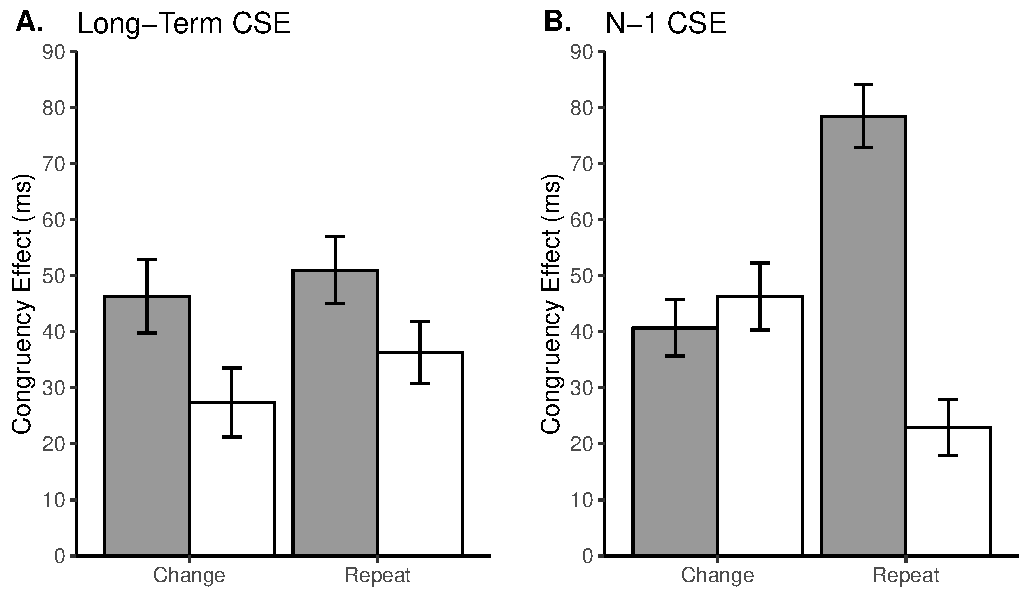
\includegraphics[height=2.75in]{figures/MGfigure5.pdf}
  \caption{Results of the stimulus-response repetition analyses}
  \caption*{Figure \ref{MG_figure5}A shows congruency effects in reaction times collapsed across all experiments as a function of Prime Congruency (congruent and incongruent) and Response (change and repeat). Figure \ref{MG_figure5}B shows congruency effects in reaction times collapsed across all experiments as a function of Trial $n-1$ Congruency (congruent and incongruent) and Response (change and repeat). Error bars represent the Standard Error of the Mean (SEM).}

  \label{MG_figure5}
\end{figure}

\hypertarget{short--and-long-term-comparison-analysis}{%
\section{Short- and Long-Term Comparison
Analysis}\label{short--and-long-term-comparison-analysis}}

The results thus far suggest that the short- and long-term congruency
effects are the result of independent processes. However, to directly
test their independence, we analyzed the congruency effects on probe
trials as a function of the previous trial congruency. We collapsed
across experiments 1 and 2 and submitted the mean RTs from correct probe
trials to a repeated-measures analysis of variance (ANOVA) with prime
congruency (congruent vs.~incongruent), trial \(n-1\) congruency
(congruent vs.~incongruent), and trial \(n\) (probe) congruency
(congruent vs.~incongruent) as factors. Two participants were removed
prior to the analysis due to missing data.

The critical three-way interaction, was non-significant,
\(F(1, 188) = 1.55\), \(\mathit{MSE} = 4,320.43\), \(p = .214\),
\(\hat{\eta}^2_p = .008\), 90\% CI \([0\), \(0.04]\). Furthermore, the
two-way interaction between trial \(n-1\) and trial \(n\) (probe)
congruency was significant, \(F(1, 188) = 8.64\),
\(\mathit{MSE} = 4,566.08\), \(p = .004\), \(\hat{\eta}^2_p = .044\),
90\% CI \([0.01\), \(0.1]\), and the two-way interaction between prime
and trial \(n\) (probe) congruency was also significant,
\(F(1, 188) = 6.62\), \(\mathit{MSE} = 3,742.42\), \(p = .011\),
\(\hat{\eta}^2_p = .034\), 90\% CI \([0\), \(0.09]\). Therefore, the
presence of the long-term congruency sequence effect did not depend on
the previous trial congruency.

\hypertarget{general-discussion-1}{%
\section{General Discussion}\label{general-discussion-1}}

The current study investigated whether congruency sequence effects could
be observed on a long-term basis. Across experiments 1 and 2, congruency
effects were significantly smaller on probe trials when the prime was
incongruent versus congruent. Long-term congruency sequence effects were
demonstrated with an average of eight intervening trials (experiment
one), and 160 intervening trials (experiment two); and were observed in
both response-repeat and response-change trials. In experiment 3, when
specific colors assigned to prime stimuli were not repeated when
presented as probes, we failed to find long-term congruency sequence
effects.

In addition to the long-term congruency sequence effect we also found
the traditional \(n-1\) congruency sequence effect. However, the \(n-1\)
sequence effect was only observed in experiments including a
high-conflict manipulation. Last, the \(n-1\) congruency sequence effect
was only found for response repeat trials and not for response change
trials, suggesting that these effects could be explained entirely by
stimulus-response repetitions.

The finding that a single presentation of a unique stimulus can
influence performance on the second, much later presentation, is
consistent with the instance-based memory account. Per this account, the
attentional priorities adopted in the presence of unique stimulus
features on the prime trial were retrieved and reinstated when those
features were presented again. This work contributes to a small, but
growing body of evidence suggesting that adjustments in cognitive
control processes like attention can be guided by memory representations
(Awh et al., 2012; Egner, 2014; Hutchinson and Turk-Browne, 2012).
Memory influences on cognitive control have largely been studied in the
context of negative priming (D'Angelo and Milliken, 2012; Frings et al.,
2015) and visual spatial attention using visual search tasks (e.g., Chun
and Jiang, 1998, 2003; Hutchinson and Turk-Browne, 2012). Our findings
complement and extend this prior work demonstrating long-term memory can
influence selective attention in a conflict task.

Although the instance-based memory account provides one explanation for
the current results, we now discuss other accounts of the congruency
sequence and proportion congruent effects and the implication of our
findings. Whether modulations of congruency effects indexes adjustments
in cognitive control or instead, emerges from lower level learning and
memory processes, remains one major point of disagreement. We have
organized our discussion around these two perspectives.

\hypertarget{control-perspectives}{%
\subsection{Control perspectives}\label{control-perspectives}}

\hypertarget{expectation-and-voluntary-control-accounts.}{%
\subsubsection{Expectation and voluntary control
accounts.}\label{expectation-and-voluntary-control-accounts.}}

The expectation account postulates that participants develop
expectations about the congruency of upcoming trials and engage in
compensatory voluntary control strategies (Gratton et al., 1992; Logan
and Zbrodoff, 1979). For example, the \(n-1\) congruency sequence effect
could reflect deliberate controlled adjustments following participants'
expectation that trial \(n\) will be the same congruency as trial
\(n-1\) (Gratton et al., 1992). In proportion congruent designs,
participants could become aware that the trials are mostly congruent or
mostly incongruent and then engage in global control strategies in
anticipation of the more likely item type (Logan \& Zbrodoff, 1979).

It is possible that setting voluntary attentional priorities could
explain the long-term congruency effect. For example, when a stimulus is
presented, participants might expect the stimulus will repeat and
prepare a strategy for the next time they see that stimulus. When that
stimulus is presented a second time, they would then voluntarily adopt
the prepared strategy. However, this proposal relies on several
assumptions that make such an explanation unlikely.

First, we must assume participants had become aware that each prime
stimulus would be repeated as a probe. Although awareness was not
measured in the current experiments, participants in experiment 1 could
easily have noticed that primes are repeated as probes every five to
eleven trials. However, in experiment 2 all the prime trials were
presented first, followed by all the probe trials. Therefore, during the
prime block, participants have no reason to expect stimulus repetition,
and during the probe block, once stimuli start repeating, it would be
too late to rely on previously unprepared stimulus-specific voluntary
strategies. Second, participants would have to actively maintain
multiple stimulus-specific strategies simultaneously. In experiment 1,
they would have to maintain 5 to 11 at any given point and in experiment
2 they would need to maintain 160. Although it is unknown how many
stimulus- or context-specific voluntary strategies can be maintained
simultaneously, 160 seems implausible. Finally, participants would have
to rapidly adjust attentional control in a voluntary manner at the time
of stimulus onset. However, voluntary control is traditionally thought
of as slow and effortful (Shiffrin and Schneider, 1977). Taken together,
the expectation or voluntary control account is not a viable explanation
of the long-term congruency sequence effects.

\hypertarget{conflict-monitoring-accounts.}{%
\subsubsection{Conflict-monitoring
accounts.}\label{conflict-monitoring-accounts.}}

According to the conflict-monitoring model, modulations of congruency
effects reflect conflict-driven adjustments in cognitive control
(Botvinick et al., 2001). That is, the detection of response-conflict --
the simultaneous activation of competing responses -- triggers an
up-regulation of cognitive control which biases attentional priority
towards the target dimension and away from the distractor dimension.
Thus, the influence of the distractor dimension is reduced following a
high-conflict, incongruent trial producing the congruency sequence
effect.

The conflict-monitoring model and many of its variants (e.g., Botvinick,
2007; Braver, 2012; Dreisbach and Fischer, 2012; Egner, 2008; Hazeltine,
Lightman, Schwarb, and Schumacher, 2011; Jiang et al., 2014) are
incapable of explaining the long-term congruency effects for the same
reasons that they have difficulties explaining item- and
context-specific proportion congruent effects. Namely, adjustments in
control operate on task-level representations, pre-specified by the
model as relevant versus irrelevant. For example, in a Stroop task, the
detection of conflict would trigger an attentional bias toward the
task-relevant dimension of color, regardless of the item presented. Of
course, item- and context-specific proportion congruent effects, and now
the long-term congruency sequence effect, demonstrate that control can
be adjusted differentially for specific items. Traditional
conflict-monitoring models cannot discriminate between items while
detecting conflict or adjusting control, and therefore, cannot produce
item-specific effects.

The adaptation-by-binding account proposes one remedy: aggregate
conflict-driven learning at the level of item features (Blais et al.,
2007; Verguts and Notebaert, 2008, 2009). Like other conflict-monitoring
accounts, the detection of response conflict provides a signal that
task-relevant connections should be strengthened. In contrast to the
previous models however, this is accomplished through a Hebbian learning
rule that only strengthens connections between active representations.
Representations consist of item-level features (e.g., the color red, the
word `BLUE'), and considered active if they are task-relevant and
currently presented. Therefore, item-specific features can selectively
become associated to the current task representation if it is frequently
paired with conflict. Such computational models have been successful in
simulating item-specific proportion congruent effects as well as more
generalized forms of the congruency sequence effects (Blais et al.,
2007; Verguts and Notebaert, 2008, 2009).

The adaptation-by-binding account may be able to produce the long-term
congruency sequence effects, but doing so may stretch the model beyond
its plausible limits. For example, it is not clear whether the model
could produce single-trial, long-term learning, or whether repeated
presentations are required to produce measurable changes in performance.
Additionally, the irrelevant contextual features that defined the unique
stimuli would need to be considered `task-relevant' by the model for
them to be active during learning. Each unique stimulus would also need
to receive its own input layer in which case the model would require at
most 160 input layers. The stimulus-set is never specified prior to the
experiment so we would also have to assume that each new stimulus
presented creates the new required input layers. If we accept these
assumptions, it is possible that the model could produce the long-term
congruency sequence effects. However, it is not clear that this model is
compatible with these assumptions. Furthermore, once these additional
assumptions are made, it is not clear how different this account is from
the instance-based memory account.

\hypertarget{conflict-monitoring-with-memory-selection.}{%
\subsubsection{Conflict-monitoring with memory
selection.}\label{conflict-monitoring-with-memory-selection.}}

We propose a new alternative conflict-monitoring model that could
account for the long-term congruency sequence effect. The congruency
task literature has had difficulty explaining why cognitive control
adjustments have been demonstrated to be at times, specific, failing to
generalize (e.g., item-specific), and at other times, nonspecific,
successfully generalizing across stimuli (e.g., Abrahamse et al., 2016;
Braem et al., 2014; Egner, 2014). The conflict-monitor, as specified by
traditional accounts (Botvinick et al., 2001; Braver, 2012) can detect
response conflict and aggregate recent or frequent conflict within a
conflict-signal, but lacks the ability to select what experiences are
aggregated or the ability to preserve multiple conflict signals. To
incorporate the ability to select and store multiple conflict signals
into the conflict monitor is problematic because it would require the
monitor to know in advance, what items should be aggregated over and
which signals preserved (Egner, 2008).

Instead, we suggest a memory-retrieval process could provide a mechanism
by which prior experiences are selected and then aggregated over by a
conflict-monitor. For example, the word `RED' in blue ink, would cue the
retrieval of any other similar experiences: any trial containing the
word `RED' or the color blue. The conflict-monitor then detects and
aggregates the conflict across the retrieved item-set and adjusts
control accordingly. By offloading the selection to a memory system, the
conflict-monitor does not need to distinguish between items and can bias
attentional priority along task-dimensions, as originally specified
(Botvinick et al., 2001). However, by allowing memory to select what
prior experiences are evaluated by the conflict-monitor, the model
becomes extremely flexible in determining when control should be
adjusted.

Such an account for example, can easily explain item- and
context-specific proportion congruent effects. In a typical
item-specific design (e.g., Jacoby et al., 2003), items are organized
into two distinct sets associated with different proportions of
congruency (e.g., the words `RED' and `BLUE' could be high proportion
congruent, and the words `GREEN' and `YELLOW' could be low proportion
congruent). Importantly, the individual features do not overlap between
item sets (though, see Bugg and Hutchison, 2013; Bugg et al., 2011). For
example, if the word `RED' is the high proportion item set and the word
`GREEN' in the low proportion, then the word and/or color red will never
be presented with the word and/or color green. Presenting `RED' in blue
will then only cue the retrieval of items from the high proportion item
set. Similarly, items that appear in one context will be associated to
items that have also appeared in that context by virtue of their shared
contextual features (e.g., same location). Therefore, context-specific
effects (Crump et al., 2006), including generalization to frequency
unbiased items (Crump et al., 2017; Crump and Milliken, 2009; Weidler
and Bugg, 2016) would also be predicted by such an account. Similarly,
memory retrieval could contribute to traditional congruency sequence
effects if we accept that that more recent memories are more easily
retrievable than distant memories (e.g., Egner, 2014).

There are however, some potential remaining issues. For example,
memory-based theories beg questions about the active features and/or
dimensions controlling memory retrieval. Prior work in the item-specific
proportion congruent literature has suggested that single features,
rather than conjunctions of features, drive proportion congruent effects
(e.g., Bugg and Hutchison, 2013; Jacoby et al., 2003). Similarly,
context-specific transfer effects suggest that single, context-features
can also drive memory retrieval (e.g., Crump and Milliken, 2009; Crump
et al., 2017; Weidler and Bugg, 2016). In the current study, we found
long-term congruency sequence effects when stimuli shared contextual
features. We only found this effect however, when stimuli appeared in
the same color set (experiments 1 and 2). When the prime and probe
appeared in different colors (experiment 3) we failed to find evidence
for the long-term congruency effect. These findings suggests that the
conjunction of features may have served as a retrieval cue in the
current study. A task for future work is to clarify the conditions that
enable a feature or conjunction of features to drive retrieval.

\hypertarget{non-control-perspectives}{%
\subsection{Non-control perspectives}\label{non-control-perspectives}}

Although the control perspective remains popular, several accounts have
challenged the underlying premise that modulations of the congruency
effect index cognitive control adjustments. Instead, some have argued
that learning and memory processes could produce the same effects
without the need for notions of conflict-driven control (Mayr et al.,
2003; Schmidt, 2013; Schmidt and Besner, 2008). For example, many
congruency task designs contain item- or feature-repetition biases that
are confounded with congruency manipulations. These confounds have
produced alternative explanations of congruency phenomena, two of which
are of importance to the current study.

\hypertarget{contingency-learning.}{%
\subsubsection{Contingency learning.}\label{contingency-learning.}}

First, the contingency learning account suggests that the frequency of
item presentation can produce predictive relationships between item
features and responses. Responses are thought to be speeded for stimuli
that contain features that are highly predictive of a response
regardless of congruency. For example, if the word `BLUE' is most often
presented in red ink, then the word `BLUE' becomes predictive of the red
response, and responses would be quicker relative to non-predictive
items. In many proportion congruent designs, the frequency of item
presentation is confounded with the proportion congruent manipulations.
Therefore, the contingency learning account has been sufficient for
explaining many proportion congruent effects, although still unable to
explain transfer to frequency unbiased items (Crump et al., 2017;
Weidler and Bugg, 2016). In the current study, however, we used a
two-choice flanker task and all potential contingencies were held
constant. That is, there were no predictive relationships between
stimulus features and responses that could explain our results.

\hypertarget{stimulus-specific-repetition-priming-and-feature-integration.}{%
\subsubsection{Stimulus-specific repetition priming and feature
integration.}\label{stimulus-specific-repetition-priming-and-feature-integration.}}

The stimulus-specific repetition priming account was proposed to explain
congruency sequence effects. Mayr, Awh, and Laurey (2003) noted that the
frequency of complete stimulus-response repetitions in trial-to-trial
transitions are unbalanced in two-choice congruency tasks. Specifically,
some congruent-to-congruent and incongruent-to-incongruent transitions
contain complete stimulus-response repetitions which could speed
responses selectively for those conditions (Hommel, 1998; Pashler and
Baylis, 1991). Consistent with this proposition, Mayr et al.~found that
the congruency sequence effect disappeared when response repetition
trials were either removed from the analysis, or prevented from
occurring in the trial sequence. Though, many studies have now
demonstrated congruency sequence effects while controlling for
stimulus-response repetitions suggesting stimulus-response repetitions
cannot entirely account for sequential effects (Akçay and Hazeltine,
2008; Kerns et al., 2004; Kunde and Wühr, 2006; Ullsperger, Bylsma, and
Botvinick, 2005; Weissman, Jiang, and Egner, 2014).

To determine whether stimulus-response repetitions played a role in
producing the current result we compared response repeat to response
change trials. We found an overall long-term response repetition effect,
in that performance was facilitated when responses repeated from prime
to probe trials. However, the size of the long-term congruency sequence
effect did not differ between response repeat and change trials
suggesting that the current result could not be explained by
stimulus-response repetitions.

The feature integration account makes a similar proposal. According to
this account, stimuli and responses that co-occur in time are bound
together in a common episodic memory representation called an event file
(Hommel, 1998; Hommel et al., 2001, 2004); a more general form of the
`object file' proposed by Kahneman, Treisman, and Gibbs (1992). The
subsequent re-occurrence of any features automatically retrieves the
entire event file which could either help or hinder performance
depending on the match between the currently presented features and the
features contained in the event file. Across two consecutive trials,
features are either completely matched, partially matched, or completely
mismatched.

Critically, an effortful `unbinding' process is necessary whenever
features are partially matched. That is, feature representations must be
unbound from the associated event file so that they can be re-used in
the creation of a new event file. Therefore, performance would be
predicted to be slowed on partial match trials relative to complete
match or complete mismatch trials. In many congruency task designs,
feature overlap is confounded with congruency sequences and as such,
feature integration can explain trial-to-trial effects in many cases
(for reviews, see Egner, 2007, 2014). Similarly, experiments 1 and 2, we
utilized a two-choice flanker task that contains these same feature
overlap confounds.

Event files are typically referred to as `transient' or `temporary'
memory structures (Hommel, 1998; Hommel et al., 2001, 2004), and are
generally invoked to explain short-term, trial-to-trial effects (Egner,
2007, 2014). However, event files are based on instance-based memory
theories (Hintzman, 1986; Logan, 1988b, 1990), and typically, the
timescale is not explicitly defined. If we assume that event files are
stable episodic memory structures, then feature integration, like the
other memory-retrieval accounts proposed above, could also explain
long-term congruency sequence effects. The evidence for long-term
feature integration across our experiments however, is mixed and largely
inconclusive.

On the one hand, across experiments one and two we found long-term
congruency sequence effects for response-change trials. This result is
generally inconsistent with feature integration theories. One
possibility, as others have suggested, is that event files may not be
limited to stimulus-response associations. That is, other aspects of an
experience like perceived conflict and control processes may also be
encoded in the event file (Bugg and Hutchison, 2013; Spapé and Hommel,
2008). We could speculate that the added contextual features could have
provided additional support for event file retrieval, even in the
absence of response repetitions (for a similar proposal, see Spapé \&
Hommel, 2008), or perhaps response outcomes are forgotten more rapidly
than degree of conflict. On the other hand, in experiment three we
failed to find long-term congruency sequence effects when colors did not
repeat from prime to probe trials. This result is consistent with
feature integration theory. Although our speculation about why we found
long-term effects in response-change trials could have also applied
here, so these two results are at odds. Furthermore, any memory-based
explanation might predict that altering the similarity between the prime
and probe trials would influence the long-term effects. Therefore, the
failure to find long-term effects when colors do not repeat, does not
allow us to discriminate between any of the memory-based theories we
have proposed. Finally, to the extent that you allow event files to be
permanent memory representations and allow them to encode many aspects
of our experience like stimulus and context features, responses,
perceived conflict, and control processing, it is not clear how
different feature integration theories are from instance-based memory
theories.

\hypertarget{perceptual-learning-and-attentional-control.}{%
\subsubsection{Perceptual learning and attentional
control.}\label{perceptual-learning-and-attentional-control.}}

Finally, we propose an alternative non-control account. Perceptual
learning refers to experience-dependent changes in perception and is
thought to reflect perceptual or neural plasticity in visual
representations (Goldstone, 1998; Lu, Hua, Huang, Zhou, and Dosher,
2011; Roelfsema, Ooyen, and Watanabe, 2010; Sasaki, Nanez, and Watanabe,
2010). Perceptual learning has been demonstrated across a wide variety
of perceptual tasks including the discrimination and detection of
stimulus orientation (Dosher and Lu, 1998; Shiu and Pashler, 1992;
Vogels and Orban, 1985), motion direction (Ball and Sekuler, 1987; Ball,
Sekuler, and Machamer, 1983) , and object recognition (Furmanski and
Engel, 2000), to name a few (for a review, see Watanabe and Sasaki,
2015). Importantly, across tasks, selective attention has been shown to
influence perceptual learning, such that learning is enhanced for
task-relevant, or attended features as compared to irrelevant,
unattended features (Ahissar and Hochstein, 1993; Gutnisky, Hansen,
Iliescu, and Dragoi, 2009; Shiu and Pashler, 1992; Szpiro and Carrasco,
2015).

One possible explanation of the long-term congruency sequence effect is
that selective attention influences perceptual learning on the first
presentation, which in-turn, influences how the stimulus is attended on
the second presentation. For example, when presented with an incongruent
stimulus, attention is shifted towards the target and away from the
flankers facilitating perceptual learning of the target features
relative to the flanker features. On the second presentation, the
altered visual representation and enhanced perceptual processing of the
target could cue attention towards the target, facilitating performance
if the second presentation is incongruent.

There is some evidence that increased selective attention demands from
incongruent stimuli may enhance target representations on a long-term
basis. As noted earlier, in perceptual learning tasks, learning is
enhanced for attended versus unattended features (Ahissar and Hochstein,
1993; Gutnisky et al., 2009; Shiu and Pashler, 1992; Szpiro and
Carrasco, 2015). However, recognition memory has also been shown to be
improved for items previously presented with incongruent versus
congruent distractors. Here, the increased need for cognitive control is
thought to facilitate target encoding at the time of study improving
later memory recognition (Krebs, Boehler, De Belder, and Egner, 2013;
Rosner et al., 2015; Rosner and Milliken, 2015).

Perceptual learning could provide an important mechanism for informing
how attention changes through experience and learning. Perceptual
learning has been shown to be highly stimulus-specific and produces
long-lasting effects (Watanabe \& Sasaki, 2015). Though in contrast to
the immediate effects in our study, measuring changes in performance on
perception tasks often requires extensive training (Dosher and Lu,
1999). Therefore, changes in perception alone could not account for the
current results. Instead, we are suggesting that small changes in
perceptual representations could help guide attention, causing more
immediate and measurable effects in attention tasks.

\hypertarget{short--and-long-term-congruency-sequence-effects-single-or-multiple-processes}{%
\subsection{Short- and long-term congruency sequence effects: Single or
multiple
processes?}\label{short--and-long-term-congruency-sequence-effects-single-or-multiple-processes}}

In the current experiments, we found both short- (n-1) and long-term
congruency sequence effects. All current accounts of the short-term
congruency sequence effects posit rapidly decaying representations and
are generally incapable of accounting for the long-term congruency
sequence effects (Egner, 2007). The alternative accounts we have
proposed above however, could accommodate both long- and short-term
effects. For example, if memory retrieval mediates shifts in attentional
control then we might expect that similarity in temporal context could
cue retrieval (e.g., Egner, 2014). One possibility is that both short-
and long-term effects are produced via a single, memory-driven process.
Alternatively, we might speculate the contribution from two independent
processes: A memory-driven process and a short-term, conflict-driven
process.

On the one hand, there were some clear differences between the short-
and long-term effects found in the current study. First, the long-term
effects were insensitive to increased response conflict, whereas the
short-term effects were only present in the high conflict experiments.
This might be expected, if we assume that the short-term effect reflects
changes in the conflict-signal which dissipates over time (e.g.,
Botvinick, et al., 2001). Second, the long-term effects were present for
both response change and response repeat trials while the short-term
effects were only present for response repeat trials. As such, the
short-term effect could be explained entirely by stimulus-response
repetitions (e.g., Mayr et al., 2003), while the long-term effect
cannot. Third, and most importantly, we found no interaction between the
short- and long-term effects. Taken together, these differences suggest
that the two phenomena measured in the current study do not reflect the
same underlying process.

On the other hand, several other studies have reported \(n-1\)
congruency sequence effects while controlling for repetition biases
(e.g., Kunde and Wühr, 2006; Weissman et al., 2014), and others have
found \(n-1\) congruency sequence effects to be insensitive to changes
in the degree of conflict (e.g., Weissman and Carp, 2013). One possible
resolution to these inconsistencies, is that a memory-driven process
can, under the right circumstances, contribute to short-term congruency
effects. That is, if the stimuli presented on trial \(n\) provides an
effect retrieval cue for trial \(n-1\), then we might expect that a
memory-driven process could influence performance on trial n.~Of course,
if trial \(n\) is a poor retrieval cue for trial \(n-1\), then we might
expect no influence from the memory-retrieval process, leaving only the
short-term, conflict-driven effect. In the current study, we alternated
the context trial-to-trial such that the same contextual cue never
repeated from trial \(n-1\) to trial n.~Therefore, it could be the case
that trial n, while an effective retrieval cue for the prime trial
(e.g., \(n-8\), \(n-160\)), was a poor retrieval cue for trial n-1. As
such, the short-term effects observed in the current study reflect only
the influence of a short-term, conflict-driven process, which was
sensitive to the degree of conflict, and response repetition.

Consistent with this interpretation, Spapé and Hommel (2008) found that
the \(n-1\) congruency sequence effect was eliminated on trials that
alternated contextual cues, but preserved when contextual cues repeated.
The authors suggested that the alternation of contextual cues
selectively disrupted episodic retrieval on those trials. However,
others have found \(n-1\) congruency sequence effects with non-repeating
contextual cues (e.g., Egner et al., 2010; King et al., 2012). One
possibility is that the combination of making a single prior experience
(the prime trial) distinctly similar to trial \(n\) and the
non-repeating contextual cues, could have disrupted memory retrieval of
the \(n-1\) trial. This would also suggest that memory retrieval in this
context, is a competitive process, whereby only the most similar
experiences are retrieved. What constitutes an effective versus
ineffective retrieval cue however, remains unclear. Furthermore, whether
only a single, most-similar previous experience is retrieved, or if a
collection of similar experiences is aggregated over and used to guide
attention remains an open question.

\hypertarget{broader-implications}{%
\section{Broader implications}\label{broader-implications}}

A global aim of this research program is to determine how memory for
specific prior experiences guides performance in the present moment.
Previous work has focused on evidence that contextual cues can rapidly
modify cognitive control settings. The instance-based memory account of
contextual control (Crump, 2016) is the general hypothesis that memory
not only preserves a record of the details of specific experiences
(Hintzman, 1986; Jacoby and Brooks, 1984; Logan, 1988b), but also
preserves a record of the control procedures involved in processing
those experiences (Kolers and Roediger, 1984). Our aim here was to
supply evidence showing that attentional control in the present moment
can be modified on a long-term basis by memories of specific prior
processing experiences. Beyond the implications of this finding for
theories of cognitive control from the congruency literature, we are
optimistic the idea behind our results will spur more work into the
memorial basis of cognitive control. In everyday life, we expect that
memory for prior cognitive control operations routinely optimizes
performance in familiar environments. In these situations, people gain
the benefit of applying memory-based procedures for regulating
information without the normal cost of effortful deliberation. We also
expect that problems in regulating the flow of information can result
from the inappropriate use of, or failure to rely on memory. For
example, deliberate control may need to override memory based control
when situations act as strong cues for prior memory procedures that may
not be appropriate for the present moment. Or, when memory fails to
encode or retrieve cognitive control procedures, people may be forced to
rely on taxing voluntary control processes to supply the control they
normally receive from memory for free. The present results show that
some aspects of the attentional control procedures used during a
fleeting encounter with a unique stimulus in a flanker task have
long-term influences on responding to that stimulus in the future.
Everyday life presents many more fleeting and meaningful experiences,
and the capacity of memory to preserve and reinstate past control
procedures to regulate cognition, behavior, and performance points to a
healthy avenue for future work.

\FloatBarrier
\newpage
\fancyhead[L]{CONTEXTUAL RECRUITMENT OF SELECTIVE ATTENTION}
\fancyhead[R]{\thepage}
\fancyfoot[C]{}

\chapter{CONTEXTUAL RECRUITMENT OF SELECTIVE ATTENTION CAN BE UPDATED VIA CHANGES IN TASK-RELEVANCE}

\hypertarget{preface-2}{%
\section{Preface}\label{preface-2}}

This chapter is reproduced from a manuscript currently under review (for
consistency, I have adjusted the format of the manuscript for the
thesis). The full reference to the article:

\vspace{1.5em}

\noindent \textbf{Brosowsky, N.P.}, \& Crump, M.J.C. (2019, January 15).
Contextual recruitment of selective attention can be updated via changes
in task-relevance. \url{https://doi.org/10.31234/osf.io/43tj7}
\vspace{1.5em}

Chapter 4 presents an experiment that examines the role of
task-relevance in producing and updating context-specific control.
Context-specific attentional phenomena demonstrate that prior
experiences and context cues can automatically trigger adjustments in
attentional control independent of awareness and intentions. Although
this finding seems plausible in a laboratory task where there is only a
single context cue (e.g., location), it is unclear how such a process
would operate in more complex, real-world environments that contain a
multitude of contextual features. That is, what determines which context
features in my environment are used to guide attention? In this
experiment, we asked whether task-relevant context cues will trigger
adjustments to attention in the presence of competing irrelevant context
cues. And whether changes in the relative task-relevance will cause
changes contextual control.

We adopted a paradigm similar to the context-specific proportion
congruent (CSPC) transfer design. However, unlike previous CSPC designs
where contexts were defined by a single discriminating feature (e.g.,
upper vs.~lower screen locations), contexts were defined by two feature
dimensions (see Figure \ref{TRfigure1}A) and critically, the frequency
unbiased context (50\% congruent) always shared a feature with each of
the frequency-biased contexts (0\% and 100\% congruent). To manipulate
which overlapping feature was task-relevant, we used a secondary
counting task. Halfway through the experiment participants received new
instructions, changing which feature was task-relevant. Across three
different stimulus sets, we found that changing the task-relevance
caused predictable changes in the congruency effects. This result
implicates an important role for task-relevance in producing and
manipulating context-dependency in complex environments.

\hypertarget{abstract-2}{%
\section{Abstract}\label{abstract-2}}

Evidence across a wide variety of attention paradigms shows that
environmental cues can trigger adjustments to ongoing priorities for
attending to relevant and irrelevant information. This context-specific
control over attention suggests that cognitive control can be both
automatic and flexible. For instance, in selective attention tasks,
congruency effects are larger for items that appear in a context
associated with infrequent conflict than in a context associated with
frequent conflict. Since the to-be-presented context cannot be predicted
or prepared for in advance, attention is assumed to be rapidly updated
on-the-fly, triggered by the currently presented context.
Context-specific control exemplifies how learning and memory processes
can influence attention to enable cognitive flexibility. However, what
determines the use of previously learned associations still remains
unclear. In the current study, we examined whether task-relevance would
influence the learning and use of context cues in a flanker task. Using
a secondary counting task, context dimensions associated with differing
levels of conflict were made task-relevant or -irrelevant across the
experiment. In short, we found that making new contextual information
task-relevant caused participants to ignore a previously learned
context-attention association and adopt a new context-specific control
strategy; all without changing the experimental stimuli. This result
suggests that task-relevance is a key determinant of context-specific
control.

\hypertarget{introduction-2}{%
\section{Introduction}\label{introduction-2}}

Selective attention is commonly investigated using interference
paradigms such as the Stroop (1935) and flanker (Eriksen and Eriksen,
1974) tasks, where participants identify a target while ignoring a
response-congruent or -incongruent distractor. Performance is typically
better on congruent versus incongruent trials and the difference---the
congruency effect---taken as an index of attentional priorities. Large
congruency effects are thought to reflect ineffective filtering of the
distracting stimuli whereas small congruency effects are thought to
reflect effective filtering. By probing factors that systematically
alter congruency effects, we can then make inferences about processes
that control attentional filtering. For example, manipulating the
frequency of conflict via the proportion of congruent versus incongruent
trials has shown to influence the size of the congruency effect.
Typically, a high proportion congruent experiment produces large
congruency effects, whereas a low proportion congruent experiment
produces small congruency effects (Logan and Zbrodoff, 1979; Lowe and
Mitterer, 1982; West and Baylis, 1998). This result is usually explained
as strategic control, where participants increase attentional control
under high-conflict demands and relax attentional control under
low-conflict demands (Logan, 1980; Logan and Zbrodoff, 1979; Logan et
al., 1984; Lowe and Mitterer, 1982). Recent work however, has
demonstrated that attentional control is not only adjusted by top-down
regulation, but can also be triggered automatically by environmental
cues (Brosowsky and Crump, 2018; Bugg and Crump, 2012; Egner, 2014;
Fischer and Dreisbach, 2015; King et al., 2012; Mayr and Bryck, 2007).

For example, Crump, Gong, and Milliken (Crump et al., 2006; see also,
Corballis and Gratton, 2003) presented Stroop stimuli in one of two
randomly chosen locations and manipulated the frequency of conflict
associated with each location. One location was associated with a high
frequency of conflict (25\% congruent trials) and the other with a low
frequency of conflict (75\% congruent trials). Overall, the proportion
of congruent trials was 50\% and randomized such that the upcoming
location could not be predicted. Even so, congruency effects were shown
to be smaller for trials where the stimulus appeared in the high
conflict location as compared to the low conflict location. This effect,
known now as the context-specific proportion congruent effect (CSPC),
has now been replicated in a number of different selective attention
paradigms (e.g., Alards-Tomalin, Brosowsky, and Mondor, 2017; Blais et
al., 2015; Bugg, 2014; Crump, 2016; Crump et al., 2018; Fischer et al.,
2014; Hübner and Mishra, 2016).

Critical evidence however, that CSPC effects reflect context-specific
control rather than other non-control learning processes (e.g., Schmidt
and Besner, 2008), comes from work showing that CSPC effects can
transfer to frequency unbiased items (Brosowsky and Crump, 2016; Crump
and Milliken, 2009; Weidler and Bugg, 2016; Weidler et al., 2018;
though, see Hutcheon and Spieler, 2017). Crump and Milliken (2009), for
example, divided Stroop items into two mutually exclusive sets (e.g.,
RED/GREEN and BLUE/YELLOW). One set was defined as the frequency biased
set, and presented with 75\% congruency in one location, and 25\%
congruency in the other. The second set however, was presented with 50\%
congruency in both locations. Nevertheless, they found smaller
congruency effects for unbiased items presented in the high conflict
location as compared to the low conflict location.

One explanation for CSPC effects is that the repeated application of
attentional priorities in a particular context creates an associative
link in episodic memory between the attentional control procedures and
the contextual information (Abrahamse et al., 2016; Brosowsky and Crump,
2018; Crump, 2016; Egner, 2014). Once the associative link is
established, processing the context is assumed to trigger the retrieval
of previous experiences, automatically reinstating associated
attentional priorities. As a result, automatic memory-based retrieval
allows attentional priorities to be rapidly adjusted in a
context-appropriate fashion. However, the obligatory nature of
memory-based attentional control remains unclear, in particular in
situations when multiple contextual features could be used as cues for
retrieval.

For example, real-world environments offer a plethora of context cues.
Consider writing an article in a coffee shop. The coffee shop is a
complex environment with numerous context cues (e.g., pictures on the
wall, chairs, coffee, laptop), and associated attentional priorities.
Although a laptop might cue attentional processing helpful for writing,
other features of the coffee shop might cue attentional processing
related to other experiences like socializing and people-watching. Given
that all of these cues are available to set attentional priorities, what
determines which associative relationships will be used to guide
attention? On the one hand, context-based retrieval of attentional
priorities might be completely obligatory and a writer's attention would
be at the mercy of the environment. On the other hand, there is some
evidence that contextual cuing of attention is not entirely obligatory
and can be constrained by task goals, allowing the laptop to take
priority as a contextual cue over other contextual cues that are
irrelevant to the task at hand.

Prior work shows that task-relevance is necessary for establishing and
using context-attention associations. First, the most commonly used
context cue is location (Brosowsky and Crump, 2016; Corballis and
Gratton, 2003; Crump, 2016; Crump et al., 2006, 2008; Weidler and Bugg,
2016; Weidler et al., 2018). Although in some sense, the location is
irrelevant for identifying the color of a word, it seems disingenuous to
consider it completely task-irrelevant. In order to identify the target,
the participant must first identify and orient to its location on the
screen. In this is sense, it is relevant to their ability to complete
the task and furthermore, location information may receive priority
during encoding (Logan, 1998; Mayr, 1996). Similar arguments could be
made about other context features that are inherent to processing the
target stimulus, like font-type (Bugg et al., 2008) and color (Vietze
and Wendt, 2009).

Second, we are aware of only one study that has looked at task-relevance
within the CSPC literature. Crump, Vaquero, \& Milliken (2008) used a
Stroop prime-probe task where the distractor word is presented first
followed by a color patch probe. Critically, they used the shape of the
color patch probe, either a square or a circle, as the contextual
dimension; one associated with a high frequency of conflict, the other
with a low frequency. In one experiment participants were made aware of
the shape-proportion contingencies but given no additional instructions.
In the second, participants were given a secondary task to count the
number of trials that contained a square. The first experiment failed to
find evidence for context-specificity, whereas the second did. Although
not testing task-relevance directly, Cañadas et al. (2013){]} found
similar effects. In this study they used images of male and female faces
as context cues in a flanker task. When given instructions to think of
the faces as members of the gender categories they found CSPC effects,
but when given instructions to think of the faces as individuals they
did not. These results suggest that making a context dimension relevant
to the on-going task is important for producing CSPC effects.

\hypertarget{the-current-study}{%
\section{The Current Study}\label{the-current-study}}

Prior work suggests that the task-relevance of contextual information is
important for establishing new associations between context cues and
attentional priorities. Simply put, CSPC effects emerge when context
cues are somehow made relevant to the task, but do not when made
irrelevant (Cañadas et al., 2013; Crump et al., 2006, 2008). However, it
still remains unclear how task-relevance may or may not inform the use
of previously learned associations. In the current study, we examined
whether manipulating task-relevance would cause participants to ignore a
previously learned association and adopt a new context-specific control
strategy.

A flanker task was used to measure attentional control in an adapted
CSPC design (Crump et al., 2017; Crump and Milliken, 2009). Similar to
previous studies, flanker stimuli were presented in contexts associated
with differing levels of conflict (0\%, 50\%, or 100\% congruent).
However, unlike previous CSPC designs where contexts were defined by a
single discriminating feature (e.g., upper vs.~lower screen locations),
contexts were defined by two feature dimensions (see Figure
\ref{TRfigure1}A). In one condition, for example, contexts were defined
by object identity (hat or chair) and color (blue or green). Only three
out of the four possible feature combinations were presented, each
associated with a different proportion of congruent trials (0\%, 50\%,
or 100\% congruent). Critically, the frequency unbiased context (50\%
congruent) always shared a feature with each of the frequency-biased
contexts (0\% and 100\% congruent). The frequency biased contexts (0\%
and 100\% congruent) however, did not share any features (see Figure
\ref{TRfigure1}C for an example).

A secondary counting task was used to manipulate the task-relevance of
the context dimensions (Crump and Milliken, 2009) which critically,
switched halfway through the experiment. Participants were instructed to
keep a running count of one of the overlapping features (e.g., ``count
whenever a hat is presented'') which was associated with either a high
or low frequency of conflict. Halfway through the experiment they
received new instructions to count the other overlapping feature (e.g.,
``count whenever a green item is presented''). Critically, the set of
context images remained the same throughout the experiment (see Figure
\ref{TRfigure1}C for an example) and the task-relevance of the context
dimensions was the only aspect of the experiment that changed from the
first to second phases.

The critical measure of interest is the congruency effect produced in
the frequency unbiased context. If, on the one hand, task-relevance has
no impact on the use of context-attention associations we would expect
no differences between the congruency effects when the high-conflict
context dimension is made task-relevant or the low-conflict context
dimension is made task-relevant. This could occur because all three
contexts are treated as individual contexts throughout the whole
experiment (e.g., Cañadas et al., 2013). Or it could occur because
associations formed in the first block interfere with learning new
associations in the second (e.g., Brosowsky and Crump, 2016). On the
other hand, task-relevance might not only dictate how associations are
formed, but also whether learned associations are used. In this case, we
would expect smaller congruency effects when the high-conflict context
dimension is made task-relevant as compared to when the low-conflict
context dimension is made task-relevant. This would demonstrate that
participants were able to ignore a previously learned association and
adopt a new context-specific control strategy.

A secondary goal was to conceptually replicate previous findings and
test the generalizability of any task-relevance effects. Therefore, we
included three conditions that differed only in the kinds of stimuli
used to create context cues. In one condition we used face images where
context dimensions were defined by social categories, similar to Cañadas
et al. (2013). However, they found that social categorization occurred
spontaneously and it was unclear what impact that would have on the
current results. Therefore, we included another condition that used
images of simple objects where context dimensions were defined by object
features. Finally, Cañadas et al. (2013) also found that context effects
generalized to novel face images. In our third condition we used
non-repeating face exemplars to examine whether any task-relevance
effects would also generalize in our design or if learning would be
image-specific.

\hypertarget{methods-7}{%
\section{Methods}\label{methods-7}}

\begin{figure}
  \centering
  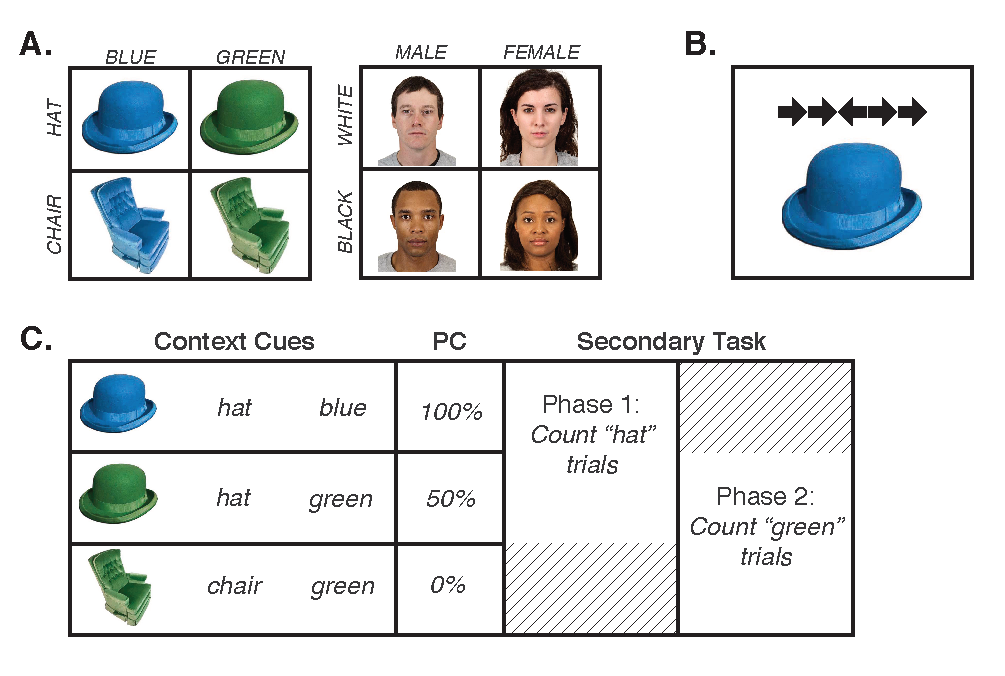
\includegraphics[width=5in]{figures/TRtask.pdf}
  \caption{Illustration of the stimuli and trial construction.}
  \caption*{Illustration of the stimuli and trial construction. Figure \ref{TRfigure1}A shows the feature dimensions for each of the conditions. Figure \ref{TRfigure1}B shows an example trial stimulus containing both the context and flanker images. Figure \ref{TRfigure1}C shows an example of how feature dimensions could have been assigned to each proportion congruency (PC) condition, and an example of the secondary task assignments. The secondary task order, as well as the feature and congruency assignments were all randomized for each participant.}
  \label{TRfigure1}
\end{figure}

\hypertarget{participants}{%
\subsection{Participants}\label{participants}}

All participants were recruited from Amazon Mechanical Turk (AMT) and
compensated \$2.00 for participating. The amount compensated was
calculated by estimating the maximum amount of time required to complete
each experiment and multiplying by \$6.00 per hour. For each experiment
the number of HITs (Human intelligence tasks, an Amazon term for a
work-unit) refers to the number of participants who initiated the study.
Participants were included in the study if they completed all trials. We
posted 150 HITs and 144 participants completed all trials.

\hypertarget{apparatus-stimuli-4}{%
\subsection{Apparatus \& Stimuli}\label{apparatus-stimuli-4}}

The experiments were programmed using JavaScript, CSS and HTML. The
program allowed participants to complete task only if they were running
Safari, Google Chrome, or Firefox web browsers. Flanker stimuli
consisted of images of five arrows pointed left or right presented at
250 x 50 pixels (each arrow was 50 x 50 pixels). Context stimuli were
constructed using images selected from Brady et al. (2013) color-rotated
to blue and green, and face images from the Chicago Face Database (Ma,
Correll, and Wittenbrink, 2015), supplemented with the NimStim Set of
Facial Expressions (Tottenham et al., 2009). The object images were
displayed at 250 x 250 pixels, while the face images were displayed at
250 x 313 pixels. The experiment ran as a pop-up window that filled the
entire screen. The background was white, and stimuli were presented in
the center of the screen.

\hypertarget{design-4}{%
\subsection{Design}\label{design-4}}

Experiment 1 used a 2x2x3 mixed design with task-relevant context (0\%
and 100\%) and unbiased-item congruency (congruent and incongruent) as
within-subject factors, and context-type (object, social, and
social/non-repeating) as the between-subjects factor. All three
conditions were constructed using the same general method. The
experiment was divided into two phases. Each phase consisted of 144
flanker trials (48 trials per context), and 13 count response trials for
a total of 314 trials. On the count response trials, participants
indicated how many trials they had counted until that point. The count
response trials occurred once for every 12 flanker trials and was
randomly inserted between trial 6 and 12 of each 12-trial block. Each
phase ended with one additional count response trial.

On every flanker trial, participants were presented with flanker stimuli
paired with one of three contexts. Each context was associated with a
different proportion congruency such that two cues were associated with
a biased frequency (0\% and 100\% proportion congruency), while one was
associated with an unbiased frequency (50\% proportion congruency). The
feature dimensions and corresponding context images assigned to each of
the biased and unbiased item sets were randomly determined for each
participant. However, context images used for the frequency biased
trials never shared features, while the frequency unbiased context image
always shared a feature with each of the frequency biased context images
(see Figure \ref{TRfigure1}). Additionally, the feature assignments
remained the same throughout phases 1 and 2, and critically, the only
change to the task was which feature the participant was instructed to
count (see Figure \ref{TRfigure1}C for an example).

All critical aspects of the task were randomized between participants.
This includes the three chosen context images, the features assigned to
proportion levels, the features assigned to each counting condition, the
secondary task order, and the order of trials.

\hypertarget{procedure-4}{%
\subsection{Procedure}\label{procedure-4}}

All participants were AMT workers who found the experiment using the AMT
system. The participant recruitment procedure and tasks were approved by
the Brooklyn College Institutional Review Board. Each participant read a
short description of the task and gave consent by pressing a button
acknowledging they had read the displayed consent form. Participants
then completed a short demographic survey, and proceeded to the main
task, which was displayed as a pop-up window. Participants were
instructed to identify the direction of the center arrow on each trial
as quickly and accurately as possible by pressing `z' if the arrow
pointed left, and `m' if the arrow pointed right. Additionally, they
were instructed to silently keep count of the number of trials that
contained a feature. In the object context condition, they were asked to
count trials that contained a certain color (blue or green) or
object-identity (hat or chair) and in the social context conditions they
were asked to count the number of trials that contained appeared a
certain gender (male or female) or race (black or white). Periodically
throughout the experiment, participants were asked to report how many
trials they had counted until that point and to restart their count from
0. Halfway through the experiment participants received new instructions
about which feature to count (see Figure \ref{TRfigure1}C).

Each trial began with a blank inter-stimulus interval (ISI) of 400 ms,
followed by a fixation cross presented in the center of the screen for
200 ms, then a second blank ISI of 400 ms. Next, the flanker and context
stimuli appeared in the center of screen (the flanker above the context
image; see Figure \ref{TRfigure1}B) and remained on screen until a
response was made. Following a response, accuracy feedback was presented
for 1000 ms. A response automatically triggered the next trial.

Halfway through the experiment (157 trials), participants received new
instructions about which feature to count and to press the button
on-screen when they were ready to continue.

\begin{figure}
  \centering
  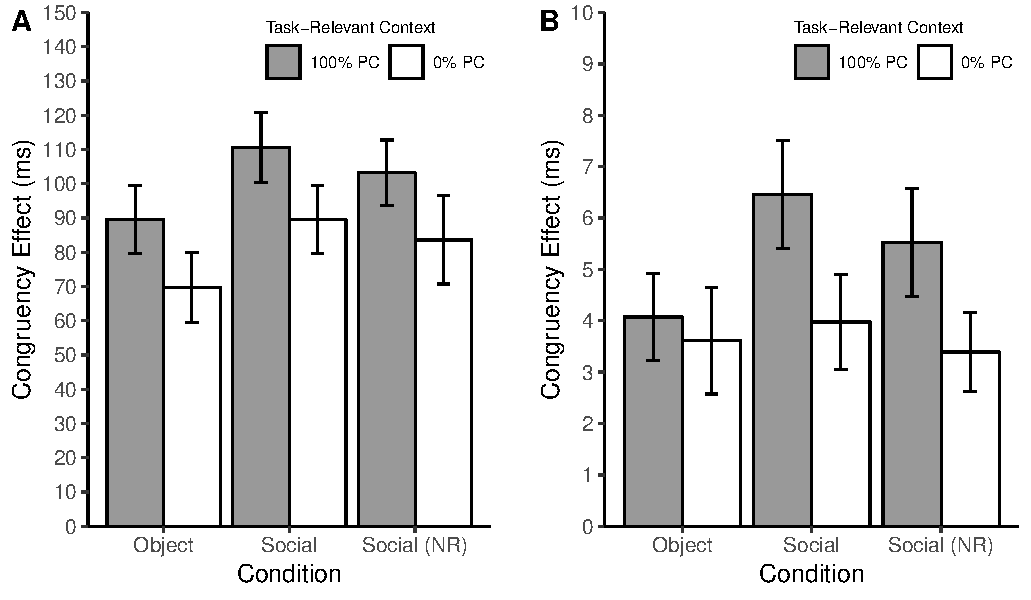
\includegraphics[width=5in]{figures/TRfigure2.pdf}
  \caption{Results from Experiment 1.}
  \caption*{Results from Experiment 1 showing congruency effects (incongruent - congruent) for frequency unbiased items in reaction times (left) and error rates (right) as a function of the task-relevant context (100\% proportion congruent versus 0\% proportion congruent).}
  \label{TR_figure2}
\end{figure}

\hypertarget{results-7}{%
\section{Results}\label{results-7}}

Participants with mean error rates greater than 25\% were excluded from
the analyses, eliminating 13 participants. For all remaining
participants, the correct RTs from frequency unbiased trials in each
condition were submitted to an outlier removal procedure. The
non-recursive Van Selst and Jolicoeur outlier removal procedure was
applied after removing response times greater than 3000 ms (Van Selst
and Jolicoeur, 1994). This procedure removed 3.39\% of the total
observations.

The primary question of interest was whether the task-relevance of
context features associated with different levels of conflict would
influence the size of the congruency effect for frequency unbiased items
(see Table \ref{TR_table}). To that end, mean correct RTs and mean error
rates from frequency unbiased trials were submitted to a mixed analysis
of variance (ANOVA) with task-relevant context (0\% and 100\% PC) and
unbiased-item congruency (congruent and incongruent) as within-subject
factors, and context-type (object, social, and social/non-repeating) as
the between-subjects factor.

The results of the RT analysis revealed the critical, two-way
interaction between task-relevant context and unbiased-item congruency
to be significant, \(F(1, 128) = 8.30\), \(\mathit{MSE} = 1,608.54\),
\(p = .005\), \(\hat{\eta}^2_p = .061\), demonstrating smaller
congruency effects when the context dimension associated with high
conflict was made task-relevant. Additionally, the three-way interaction
between the task-relevant context, unbiased-item congruency, and
context-type was non-significant, \(F(2, 128) = 0.00\),
\(\mathit{MSE} = 1,608.54\), \(p = .996\), \(\hat{\eta}^2_p = .000\),
showing no evidence for differences between the CSPC effects across
context-type manipulations (see Figure \ref{TR_figure2}).

Similarly, the corresponding error analysis also resulted in a
significant two-way interaction between the task-relevant context and
unbiased-item congruency, \(F(1, 128) = 6.72\),
\(\mathit{MSE} = 13.93\), \(p = .011\), \(\hat{\eta}^2_p = .050\), and a
non-significant three-way interaction between task-relevant context,
unbiased-item congruency, and context-type, \(F(2, 128) = 0.92\),
\(\mathit{MSE} = 13.93\), \(p = .400\), \(\hat{\eta}^2_p = .014\).
Therefore, the congruency effects in error rates were also smaller when
the context dimension associated with high conflict was made
task-relevant, corroborating the results of the reaction time analysis.

\begin{table}[htbp]
\caption{Reaction times and error rates from Experiment 1.}
\label{TR_table}
\centering
\begin{tabular}{lllcccc}
\toprule
 & & & \multicolumn{2}{c}{Congruent} & \multicolumn{2}{c}{Incongruent} \\
\cmidrule(rl){4-5}
\cmidrule(rl){6-7}
\multicolumn{1}{c}{Task-Relevant Context} & \multicolumn{1}{c}{Condition} & \multicolumn{1}{c}{PC} & \multicolumn{1}{c}{RT} & \multicolumn{1}{c}{ER} & \multicolumn{1}{c}{RT} & \multicolumn{1}{c}{ER}  \\
\midrule
\multirow{9}{*}{100\% PC} & \multirow{3}{*}{Object} & \multicolumn{1}{l}{0\%} & \multicolumn{1}{l}{-} & \multicolumn{1}{l}{-} & \multicolumn{1}{l}{693 (26)} & \multicolumn{1}{l}{4.17 (0.73)} \\
& & \multicolumn{1}{l}{50\%} & \multicolumn{1}{l}{585 (23)} & \multicolumn{1}{l}{0.74 (0.27)} & \multicolumn{1}{l}{675 (28)} & \multicolumn{1}{l}{4.81 (0.82)} \\
& & \multicolumn{1}{l}{100\%} & \multicolumn{1}{l}{587 (25)} & \multicolumn{1}{l}{0.69 (0.23)} & \multicolumn{1}{l}{-} & \multicolumn{1}{l}{-} \\
\cmidrule(rl){2-7}
& \multirow{3}{*}{Social} & \multicolumn{1}{l}{0\%} & \multicolumn{1}{c}{-} & \multicolumn{1}{l}{-} & \multicolumn{1}{l}{745 (25)} & \multicolumn{1}{l}{5.86 (0.77)} \\
& & \multicolumn{1}{l}{50\%} & \multicolumn{1}{l}{612 (21)} & \multicolumn{1}{l}{0.39 (0.19)} & \multicolumn{1}{l}{722 (26)} & \multicolumn{1}{l}{6.78 (1.04)} \\
& & \multicolumn{1}{l}{100\%} & \multicolumn{1}{l}{616 (20)} & \multicolumn{1}{l}{0.63 (0.2)} & \multicolumn{1}{l}{-} & \multicolumn{1}{l}{-} \\
\cmidrule(rl){2-7}
& \multirow{3}{*}{Social (NR)} & \multicolumn{1}{l}{0\%} & \multicolumn{1}{l}{-} & \multicolumn{1}{l}{-} & \multicolumn{1}{l}{813 (25)} & \multicolumn{1}{l}{5.04 (0.74)} \\
& & \multicolumn{1}{l}{50\%} & \multicolumn{1}{l}{689 (23)} & \multicolumn{1}{l}{0.19 (0.14)} & \multicolumn{1}{l}{793 (27)} & \multicolumn{1}{l}{5.72 (1.06)} \\
& & \multicolumn{1}{l}{100\%} & \multicolumn{1}{l}{689 (25)} & \multicolumn{1}{l}{0.48 (0.17)} & \multicolumn{1}{l}{-} & \multicolumn{1}{l}{-} \\
\midrule
\multirow{9}{*}{0\% PC} & \multirow{3}{*}{Object} & \multicolumn{1}{l}{0\%} & \multicolumn{1}{l}{-} & \multicolumn{1}{l}{-} & \multicolumn{1}{l}{649 (16)} & \multicolumn{1}{l}{3.84 (0.6)} \\
& & \multicolumn{1}{l}{50\%} & \multicolumn{1}{l}{587 (17)} & \multicolumn{1}{l}{0.56 (0.21)} & \multicolumn{1}{l}{657 (17)} & \multicolumn{1}{l}{4.17 (1.02)} \\
& & \multicolumn{1}{l}{100\%} & \multicolumn{1}{l}{634 (18)} & \multicolumn{1}{l}{2.69 (0.58)} & \multicolumn{1}{l}{-} & \multicolumn{1}{l}{-} \\
\cmidrule(rl){2-7}
& \multirow{3}{*}{Social} & \multicolumn{1}{l}{0\%} & \multicolumn{1}{l}{-} & \multicolumn{1}{l}{-} & \multicolumn{1}{l}{722 (23)} & \multicolumn{1}{l}{5.77 (0.92)} \\
& & \multicolumn{1}{l}{50\%} & \multicolumn{1}{l}{633 (20)} & \multicolumn{1}{l}{0.78 (0.5)} & \multicolumn{1}{l}{722 (25)} & \multicolumn{1}{l}{4.75 (0.9)} \\
& & \multicolumn{1}{l}{100\%} & \multicolumn{1}{l}{673 (21)} & \multicolumn{1}{l}{1.84 (0.47)} & \multicolumn{1}{l}{-} & \multicolumn{1}{l}{-} \\
\cmidrule(rl){2-7}
& \multirow{3}{*}{Social (NR)} & \multicolumn{1}{l}{0\%} & \multicolumn{1}{l}{-} & \multicolumn{1}{l}{-} & \multicolumn{1}{l}{807 (26)} & \multicolumn{1}{l}{4.55 (0.8)} \\
& & \multicolumn{1}{l}{50\%} & \multicolumn{1}{l}{735 (28)} & \multicolumn{1}{l}{0.87 (0.36)} & \multicolumn{1}{l}{818 (30)} & \multicolumn{1}{l}{4.26 (0.8)} \\
& & \multicolumn{1}{l}{100\%} & \multicolumn{1}{l}{779 (34)} & \multicolumn{1}{l}{2.03 (0.4)} & \multicolumn{1}{l}{-} & \multicolumn{1}{l}{-} \\
 & & & & & & \\
\bottomrule
\multicolumn{7}{l}{\textit{Note}: RT = Reaction Time (ms);  ER = Error Rates (\%); PC = Proportion Congruent;} \\
\multicolumn{7}{l}{NR = Non-Repeating; Standard Errors are presented in parantheses.} \\
\end{tabular}%
\end{table}

\hypertarget{general-discussion-2}{%
\section{General Discussion}\label{general-discussion-2}}

The aim of the current study was to determine whether task-relevance
plays a role in the contextual recruitment of selective attention.
Specifically, we tested whether manipulating the relative task-relevance
of context cues could cause participants to ignore a previously learned
context-association and apply a new association. We created a frequency
unbiased context cue that shared features with two frequency biased
contexts and used a feature-counting task to manipulate the
task-relevance of context dimensions across two blocks of trials.
Critically, halfway through the experiment participants received new
instructions changing the task-relevant feature from one frequency
biased cue to the other.

The key finding was that the congruency effects for the frequency
unbiased items were significantly larger when the low-conflict context
was made task-relevant as compared to when the high-conflict context was
made task-relevant. This result is consistent with prior CSPC effects
and, like the previous work, suggests that the context cues triggered
rapid adjustments to attentional control (Crump and Milliken, 2009).
However, unlike prior studies, we were able to experimentally manipulate
the CSPC effect across blocks of trials without changing any of the
physical properties of the stimuli. This novel finding demonstrates that
participants were able to learn and apply one context-attention
association in the first phase, and subsequently ignore that association
to learn a new association in the second phase.

This result implicates an important role for task-relevance in producing
CSPC phenomena. Crump et al. (2008) used shapes as context cues in a
prime-probe Stroop task and did not find CSPC effects until the context
cues were made task-relevant. Similarly, Cañadas et al. (2013)
eliminated the CSPC effect by making the contextual cue effectively
unrelated to the task. These studies suggest that task-relevance plays
an important role in establishing associations between contextual
information and attentional priorities to produce CSPC effects. Our
finding extends this work in two important ways. First, we show that
changing the task-relevance of the presented cues corresponded with a
change in attentional control in the predicted direction. This
demonstrates that task-relevance is also a key determinant of whether a
previously learned attention-context association will be used or ignored
in favor of a new association. Second, we show that task-relevance
allowed participants resolve competition between two competing
contextual cues, responding on the basis of one at the expense of the
other. To our knowledge, this is the first demonstration that CSPC
effects can be produced when there are multiple, overlapping contextual
cues available.

In light of prior work, we take this as evidence that the contextual
recruitment of selective attention, although likely implicit, is not
obligatory (e.g., Brosowsky and Crump, 2016), requiring that
environmental information be incorporated into the task representation.
Similarly, there appears to be flexibility in which environmental
features are selected and used to guide attention, which can be rapidly
updated depending on the task-relevance of those features. Such a result
lends some insight into how context-specific control might operate in
more complex, real-world environments, where there is an over-abundance
of environmental features that afford many different learned
associations. From a theoretical perspective, this result is consistent
memory-based accounts of CSPC phenomena (Brosowsky and Crump, 2018; Bugg
and Hutchison, 2013; Crump et al., 2017, 2018; Crump and Milliken,
2009). Under this view, a memory process encodes attentional priorities
in the representation of individual experiences and, as a result, become
associated with the environment where they were used. The subsequent
reoccurrence of a prior context triggers the retrieval and reinstatement
of those attentional priorities. Our results show however, that all the
features of the environment may not be treated equally and that only
task-relevant features are used to probe memory and guide attention.

Another key result of this study concerned the different stimuli used as
context cues. Across the three conditions, we varied the type of context
image and dimensions. We manipulated the type of image presented,
including both objects (identity and color dimensions) and faces (gender
and racial dimensions). We also manipulated whether a single set of
three repeating images were presented (object and social) or a set of
non-repeating images were presented (social/non-repeating). Across all
three conditions, we found no evidence that using different stimuli had
an influence on the size or direction of the CSPC demonstrating
generalizability of this phenomenon. Furthermore, CSPC effects were
present even when using non-repeating images which suggests that
context-dependency did not rely on image-specific associations but
higher-order, learned categorical information.

Traditional models of person perception posit that social categories are
automatically activated in the presence of social stimuli (e.g., Brewer,
1988; Devine, 1989; Fiske and Neuberg, 1990). Cañadas et al. (2013)
however, found that directing participants to think about faces in terms
of individual features eliminated context-specific attention effect and
suggested that momentary motivations may influence the automaticity of
social categorization. Our results add to this literature by observing
the influence of momentary motivations (i.e., task-relevance) when there
is competition between two salient social categories. Specifically, we
found that participants could categorize on the basis of one social cue
at the expense of the other, and subsequently switch between them. These
findings may speak to issues of automaticity in social categorization
(Macrae and Bodenhausen, 2001) as well as understanding how the
situational context can prime one social identity over another (Crisp
and Hewstone, 2007). Furthermore, we found no evidence for differences
between the social and object conditions. This suggests that
categorization within the CSPC task is quickly and easily learned when
the task supports such learning and is non-unique to social stimuli.

In sum, our results provide new evidence that changes in task-relevance
can update the contextual recruitment of selective attention in a CSPC
flanker task. We demonstrated that making one context cue task-relevant
produced a CSPC effect, even in the presence of a competing contextual
cue. More important however, we found that changing the task-relevance
of the contextual cues across blocks of trials was accompanied by
predictable changes in the congruency effects. These effects were found
to be generalizable across two different kinds of stimuli and occurred
even when using non-repeating images, and implicate an important role
for task-relevance in producing context-dependency and are consistent
with memory-based accounts of CSPC phenomena.

\FloatBarrier

\newpage
\fancyhead[L]{GENERAL DISCUSSION}
\fancyhead[R]{\thepage}
\fancyfoot[C]{}

\chapter{GENERAL DISCUSSION}

Modern views on selective attention and cognitive control often bin
processing into dichotomies like controlled/automatic,
top-down/bottom-up, and endogenous/exogenous. Theoretical treatments of
attention, however, have often included a third kind of attentional
control whereby attention is guided by internal memory representations
created through experience. Though they rarely elaborate on how such
memory systems would operate and instead vaguely appeal to associative
learning principles. More recent empirical work has also demonstrated
that prior experiences can influence selective attention in a seemingly
automatic, stimulus-driven manner. This evidence has been difficult to
reconcile with dichotomous frameworks of cognitive control (Botvinick et
al., 2001; Braver, 2012; Chiu and Egner, 2019; De Pisapia and Braver,
2006; Jiang et al., 2014).

Based on these theoretical and empirical gaps, I argued that there is a
need to examine attention using a memory-based framework and proposed an
instance-based memory theory. The instance theory of automatic
attentional control relies on four assumption (e.g., Logan, 1988;
Hintzman, 1984): (1) \textit{obligatory memory encoding}; (2)
\textit{"instance" or "exemplar" memory representation}; (3)
\textit{obligatory memory retrieval}; and (4)
\textit{the preservation of cognitive processing details}. The current
thesis investigated general principles of the instance theory using a
converging operations approach.

To further situate the contribution of the thesis, the following
sections will briefly discuss the findings of the empirical work and
their implications for theories of attention and cognitive control. In
the first section, I will briefly summarize the critical aspects of the
empirical findings in the thesis. Following that, I will discuss some
limitations and open questions regarding the instance theory and
automatic attentional control. Finally, I will discuss some broader
implications of the current thesis.

\hypertarget{summary-of-empirical-chapters}{%
\section{Summary of empirical
chapters}\label{summary-of-empirical-chapters}}

In Chapter 2, I investigated the obligatory nature of memory encoding of
attentional control. In the selective attention domain, the
gold-standard measures of attention are conflict paradigms, like the
Stroop (1935) and flanker (Eriksen and Eriksen, 1974) tasks. Learning
associations between context cues and selective attention, using these
tasks, are thought to occur implicitly, without awareness, and in an
obligatory fashion. However, these tasks present a very specific
situation where a distracting irrelevant dimension interferes with our
ability to attend to the relevant dimension. Here, I looked at whether
participants would learn context-specific attentional control strategies
in a novel bi-dimensional sampling task. I found participants did not
spontaneously learn context-specificity. Instead, participants had to be
instructed to adopt context-specific attentional strategies before any
learning occurred.

There were two important differences between my task and traditional
congruency tasks. First, there was no conflict between the two
dimensions, in the traditional sense, and both dimensions were
task-relevant. Second, attentional selection occurred after the
presentation of the target stimulus (e.g., Sperling, 1960). The finding
that learning was not spontaneous suggests that learning
context-attention associations is not error-driven, but requires
participants to be engaged in the attentional strategy before, or while
the target stimulus is presented.

In Chapter 3, I investigated the long-term preservation of single
experiences with conflict. One of the more distinguishing predictions
made by the instance theory is that single experiences are preserved in
the long-term and, if retrieved from memory, can produce automatic
attentional control. Most theories of automatic attentional control, in
contrast, propose that automaticity requires extensive practice (e.g.,
Schneider and Shiffrin, 1977; Shiffrin and Schneider, 1977; A. M.
Treisman, 1969). Here, I used a large set of unique context items to
determine whether a single experience applying attentional control on an
item can influence a second presentation after many intervening trials.
If so, I predicted a pattern of results similar to the congruency
sequence effect. Across three experiments I found evidence that single
experiences can influence selective attention after many intervening
trials (4 to 319). However, I also note some boundary conditions,
failing to find such effects when the repeated items differed in
superficial details (color).

In Chapter 4, I investigated how automatic attention could be controlled
by manipulating memory-retrieval via task-relevance. Automaticity,
according to the instance theory, is a memory-retrieval process. This
suggests that there should be some flexibility in whether learning is
expressed depending on which features of the environment are used to cue
memory. In this chapter, I examined whether manipulating the relevance
of context features would cause changes in context-dependent attentional
control.

I adopted a paradigm similar to the context-specific proportion
congruent (CSPC) transfer design. However, unlike previous CSPC designs
where contexts were defined by a single discriminating feature (e.g.,
upper vs.~lower screen locations), contexts were defined by two feature
dimensions and critically, the frequency unbiased context (50\%
congruent) always shared a feature with each of the frequency-biased
contexts (0\% and 100\% congruent). To manipulate which overlapping
feature was task-relevant I used a secondary counting task. Halfway
through the experiment participants received new instructions, changing
the task-relevant context feature. Across three different stimulus sets,
I found that changing the task-relevance caused predictable changes in
the congruency effects. This result implicates an important role for
task-relevance in producing and manipulating context-dependency in
complex environments.

\hypertarget{re-evaluating-the-instance-theory-of-automatic-attentional-control}{%
\section{Re-evaluating the instance theory of automatic attentional
control}\label{re-evaluating-the-instance-theory-of-automatic-attentional-control}}

The central aim of the current thesis was to evaluate general principles
of the instance theory of automatic attention as it applies to selective
attention. One fundamental question then, is whether the presented body
of empirical work provides evidence for the instance theory of automatic
attentional control. The answer, in my view, is both yes and no. The
evidence provided here certainly is \textit{consistent} with an instance
theory. Whether all possible alternative explanations can be ruled out
is more difficult to say. Part of the problem is that most theories of
automatic attention are vague, so it is difficult to determine what
kinds of predictions they would make. I do think the evidence here
however, is more consistent with the predictions made by an instance
theory than any of ther alternatives.

For one, theories of learning and attention posit practice as the single
most important pre-requisite for automaticity (e.g., Logan, 1988b;
Schneider and Shiffrin, 1977; Shiffrin and Schneider, 1977; A. M.
Treisman, 1969). Under the instance theory, the role of practice is more
nuanced. Automaticity from this perspective is not about laying down a
certain number of memory traces, but instead about how easily those
memory traces are retrieved. On the one hand, if memory retrieval is
inefficient or difficult, many memory traces might be required for
automaticity to develop. On the other hand, if a single memory is
distinctive enough to support efficient retrieval, it should produce
automatic attentional control. This is exactly what I found in Chapter
3: single, distinctive experiences were sufficient to influence
performance in a selective attention task after many intervening trials.

Second, theories of learning and attention posit that once automaticity
develops it is difficult to suppress or modify. They seem to be
suggesting, on the one hand, that automatic processes become hardwired
and the mere presence of a stimulus should trigger its associated
attentional control in a ballistic, rigid manner. On the other hand,
they also suggest that these automatic processes can be controlled under
some circumstances but do not make any predictions about when automatic
processes can be controlled or explain how (e.g., Logan, 1988b; Posner
and Snyder, 1975a, 1975b; Schneider and Shiffrin, 1977; Shiffrin and
Schneider, 1977).

The instance theory in contrast, allows associations to form between
stimuli and attentional control -- by way of encoding multiple memory
traces -- but also makes predictions about whether that learning will be
expressed in subsequent experiences which is dictated by memory
retrieval. The extent to which automaticity can be controlled then, is
determined by the extent to which memory retrieval can be controlled
(e.g., Logan, 1988; 1992). In Chapter 4, I demonstrated that
participants learned an association between contextual cues and
attentional control in the first block of trials. Then, by shifting
which features were task-relevant, demonstrated that participants could
ignore the previous block and learn a new association. This result would
be difficult to reconcile with the view that once learned, automaticity
is difficult to modify, but easily accommodated by an instance theory.
Under this view, by making some features task-relevant, I was modifying
which features of the stimuli were being used to cue memory and
dictating which prior experiences were being retrieved.

However, there is still no conclusive evidence for the instance theory's
key assumption: instance representation. Although Chapter 3 presented
evidence that single experiences can influence selective attention, this
does not provide evidence that every experience is stored in a separate
memory trace. It seems likely that associative learning could account
for all the data provided here without this assumption. Associative
learning differs from the instance theory in that learning is modeled as
the gradual accumulation of excitatory or inhibitory connections between
stimulus units. The associative strength is summative and represents the
entire history of learning (e.g., Rescorla and Wagner, 1972). If taken
at face value, this would separate learning from memory and implies that
learners do not remember the events of separate trials or experiences,
which seems quite extreme (e.g., Fagot and Cook, 2006; Miller, Barnet,
and Grahame, 1995; Vaughan and Greene, 1984; Voss, 2009). However,
others have argued that the underlying architectures of associative and
exemplar models are homogulous and the ``structures of current
associative learning being just graphical depictions of relationships
\ldots{} common to both kinds of theory'' (Estes, 1991, p. 11). In which
case the summative representation is more of a computational convenience
than a theoretical statement about memory representation. In either
case, associative learning models are similar enough to exemplar models
that they could produce the same kinds of predictions (e.g., Blough,
1998; Jamieson et al., 2012, 2010), but without assuming instance
representation.

\hypertarget{limitations-and-open-questions}{%
\section{Limitations and open
questions}\label{limitations-and-open-questions}}

\hypertarget{the-limitations-of-verbal-theories}{%
\subsection{The limitations of verbal
theories}\label{the-limitations-of-verbal-theories}}

Although the evidence is consistent with an instance theory, it is
difficult to rule out all possible alternative explanations for the data
presented. In part, this difficulty is due to the limitations of verbal
or descriptive theories. This issue is most apparent in Chapter 3, where
I discussed a variety of alternative theoretical explanations for the
long-term congruency sequence effect. The long-term congruency sequence
effect was an interesting finding that was predicted by the instance
theory. However, many theories could also accommodate the finding with
only small adjustments. This is one limitation of verbal theories:
Verbal theories are inherently flexible, open to interpretation and
difficult to falsify.

Take for example the feature integration theory of congruency sequence
effects (Hommel, 1998; Hommel et al., 2001, 2004). Here is a theory
developed to explain trial-to-trial adjustments of the congruency effect
using an event-binding model (e.g., Kahneman et al., 1992). This theory
explains congruency sequence effects as the result of a process
attempting to bind sequential events together and makes no assumptions
about long-term storage. However, because the theory does not state any
explicit assumptions about long-term preservation, it is open to
interpretation, and if one wanted to allow for long-term storage, then
it could accommodate long-term effects. In effect, both the existence
and non-existence of long-term phenomena would be consistent with this
theory.

A second, related, limitation is that verbal theories are
under-specified and do not make very precise predictions. This makes it
difficult to determine whether data are consistent with the theory. In
Chapter 3 for example, the long-term congruency sequence effect was
found when the prime and probe shared colors, but disappeared when the
colors of the images changed from prime to probe. Unfortunately, it is
not clear whether that result is consistent or inconsistent with the
instance theory. The instance theory makes the broad prediction that the
currently presented stimulus will cue the retrieval of similar items in
memory. It does not however, make precise predictions about how similar
items need to be for retrieval. So, if we accept that changing colors
reduces similarity to the point of impaired retrieval, the data are
still consistent with the instance theory.

Overall, I think the instance theory provides a good theoretical
framework to assess the role of memory in guiding selective attention.
To generate further predictions however, I think it will be necessary to
refine the theory to formulate more concrete hypotheses and finer
predictions. One possible route is to develop computational models that
better specify the hypothesized mechanisms that underlie memory
encoding, storage, and retrieval. For instance, there are open questions
about how memories are aggregated on retrieval. It is unclear from the
current theory, what to predict after multiple exposures to the same
stimulus. Some exemplar models conceptualize retrieval as a race which
retrieves a single memory trace (Logan, 1988b), others as an
accumulation of evidence, weighted by similarity (Palmeri, 1997), and
others still as similarity-based aggregation (Hintzman, 1984).
Therefore, one path forward is to use these computational models to
better refine the instance theory and generate new hypotheses.

\hypertarget{do-we-need-to-assume-attentional-control-settings-are-preserved-in-memory}{%
\subsection{Do we need to assume attentional control settings are
preserved in
memory?}\label{do-we-need-to-assume-attentional-control-settings-are-preserved-in-memory}}

One of the general assumptions of the instance theory of automatic
attentional control is that processing details are preserved in memory
(Estes, 1972; Kolers and Roediger, 1984). It is worth considering
whether this assumption is necessary to explain the influence of prior
experience on selective attention. One alternative is that associations
form between stimuli and diagnostic features of attentional priority.
For instance, a stimulus might be frequently paired with a reward. The
re-presentation of that stimulus could trigger the retrieval of prior
experiences, indicating that it was rewarded in the past, and attention
prioritizes its processing based on that retrieved reward. Here, we do
not need to assume that the attentional priority per se was stored and
retrieved, but instead the level of reward was stored and retrieved and
used as a diagnostic feature for determining attentional priority. Other
features like predictiveness and conflict could be used in a similar
manner. This approach suggests that the attentional control system uses
some set of pre-defined diagnostic features to determine priority and
when memory encodes experiences they are tagged with associated
features.

We need not stop there however. If we assume that all features of the
experience are stored in a memory trace, then prior experiences can be
evaluated on any dimension \textit{after} retrieval. That is to say we
do not need to assume that the level of reward is stored if we assume
that the stimulus, response, and outcome are stored together. Whether
the outcome was rewarding can be assessed after retrieval. Similarly, if
the word RED in a blue colored font is stored in memory, then it does
not need to store an associated level of `conflict' because it can be
evaluated for conflict after retrieval. This is actually consistent with
the conflict-monitoring model, that assumes there is a dedicated
cognitive process for evaluating the current level of conflict and
triggering adjustments in control (Botvinick et al., 2001; Braver, 2012;
De Pisapia and Braver, 2006). It need only be extended to evaluate the
conflict of retrieved prior experiences as well as the currently
experienced conflict.

In some ways, these approaches are more easily reconciled with
traditional views of controlled and automatic processes than the
instance theory. Attention, from these perspectives, is a controlled
process and does not need to become automatic. Instead, the attentional
control process leverages evidence from prior experiences to help
determine attentional prioritization. For example, if the word RED in
blue colored font retrieves many experiences that contain conflict, then
the current experience feels more conflicting than if it did not
retrieve experiences containing conflict. Attention is adjusted in
response to the experienced conflict and experienced conflict is
influenced by both the currently presented stimulus and memory. This
differs from the instance theory which proposes that an attentional
response is automatically reinstated, circumventing executive control
entirely (e.g., Logan, 2005; Moors and De Houwer, 2006; Schneider and
Shiffrin, 1977; Shiffrin and Schneider, 1977).

One inherent problem for these kinds of approaches however, is that they
do not provide a mechanism for indicating how attention should be
adjusted, only when attention should be adjusted. For example, if the
word RED in blue colored font triggers a need for control, because of
experienced/retrieved conflict, how does the attention system know that
the color dimension should be prioritized and the word dimension
ignored? The instance theory obviously does not have this issue because
attentional control priorities are stored in memory.

Additionally, the instance theory is the most general account because it
assumes all cognitive processing details are preserved. Therefore, any
cognitive control procedure can be stored and retrieved without the need
to identify specialized diagnostic features (e.g., predictiveness,
conflict) or specialized monitoring processes (e.g., the
conflict-monitor). The instance theory then, can accommodate other
cognitive control phenomena that have shown long-term contextual control
effects (e.g., visual search, task-switching, negative priming, etc.) by
appealing to the same underlying mechanisms. So although there does seem
to be plausible alternatives to the assumption that cognitive procedures
are stored and reinstated, the instance theory still seems like the most
parsimonious and general account.

\hypertarget{do-we-actually-need-three-kinds-of-attentional-control}{%
\subsection{Do we actually need three kinds of attentional
control?}\label{do-we-actually-need-three-kinds-of-attentional-control}}

Traditionally, theories of attentional control assert a dichotomy
between top-down and bottom-up control. The former reflecting current
goals and the latter reflecting physical salience of the stimuli. I, as
well as many others, have argued that there is a need for third kind of
attentional control reflecting the influence of prior experiences; an
automatic or memory-guided attentional control (e.g., Awh et al., 2012;
Egner, 2014; Failing and Theeuwes, 2018; Hutchinson and Turk-Browne,
2012). Again, here I consider whether this assumption is necessary.

One alternative, not previously entertained, is that bottom-up
attentional control and memory-guided attentional control both reflect
learned attentional priorities. Primitive physical features of our
environment like sudden onsets, loud noises, or high contrast objects,
are thought to automatically capture attention. It might be the case
that these low level features have become associated with high
attentional priority through experience. Evidence for this comes from
work showing that bottom-up attentional capture is subject to top-down
control similar to other automatic, learned behaviors (e.g., Anderson
and Folk, 2010; Eimer and Kiss, 2008; Folk, Remington, and Johnston,
1992).

Additionally, some models of attention (Kahneman and Daniel, 1973;
Schneider and Shiffrin, 1977; Shiffrin and Schneider, 1977) allow
automatic attention to interject at any point during perceptual
processing. Accordingly, early perceptual processing could cue memory
with primitive features directing attention automatically before the
stimuli are even fully processed. The strength by which some features of
our environment seem to direct our attention automatically (e.g., the
sudden appearance of a new object) might simply reflect extensive
experience or how early in perceptual processing memory is cued.
Therefore, it seems plausible, at least on the surface, that all
bottom-up attentional phenomena could reflect the same memory-retrieval
process as the one proposed here.

\hypertarget{broader-implications-1}{%
\section{Broader implications}\label{broader-implications-1}}

A global aim of this empirical work is to determine how memory for
specific prior experiences guides performance in the present moment. In
the current thesis, I have outlined a theoretical framework describing
how memory could influence cognitive control in an automatic,
stimulus-driven manner. The empirical work presented here, together with
the prior research, lends support this theory. The instance theory is a
general theory of how control processing can be preserved and
automatically reinstated. As such, it has implications for theories of
cognitive control more generally. Furthermore, a better understanding of
how memory for prior experiences can influence cognitive control may
have more practical implications.

In everyday life, we would expect that memory for prior cognitive
control operations routinely optimizes performance. When in familiar
environments, people would gain the benefit of applying memory-based
procedures for regulating the flow of information without the effortful
cost of deliberation. These insights could be important for how we think
about training in tasks where learning and attention are critically
important. For instance, an important task for airport security is to
use x-rays to screen baggage for dangerous items (e.g., Biggs and
Mitroff, 2015; McCarley, Kramer, Wickens, Vidoni, and Boot, 2004; Wolfe,
2010). This is an extremely attention-demanding task and resembles a
variety of laboratory phenomena (e.g., visual search, congruency
effects, vigilance/mind-wandering). Developing expertise could be
streamlined if we know which kinds of experiences facilitate the
development of automaticity. For instance, a few easily retrievable,
context-rich experiences might improve training compared to many,
poorly-defined experiences. Furthermore, developing generalization might
require different kinds of training procedures.

Additionally, problems in regulating the flow of information can result
from the inappropriate use of, or failure to rely on memory. For
example, deliberate control may need to override memory based control
when memory-guided procedures are inappropriate yet the environment acts
as a strong cue. Or, when memory fails to encode or retrieve cognitive
control procedures, people may be forced to rely on taxing voluntary
control processes to supply the control. Evaluating deficits in
executive functioning and cognitive control using a memory-based
framework could provide important insights from a clinical perspective.

For instance, many clinical disorders like obsessive compulsive disorder
(OCD) and attention-deficit/hyperactivity disorder (ADHD) are associated
with difficulties selectively attending, shifting attention, inhibiting
inappropriate responses, and slowed motor response. These difficulties
are typically explained as deficits in executive functioning (Olley,
Malhi, and Sachdev, 2007; Snyder, Kaiser, Warren, and Heller, 2015).
However, they could reflect deficits in memory based control. For
example, what appears to be the inability to suppress unwanted
behaviors, or to inhibit irrelevant information, might reflect an
inability to properly contextualize task-relevant information,
triggering automatic attentional responses to task-irrelevant cues.
Similarly, overall slow motor responses could reflect a failure to
retrieve cognitive control procedures, forcing people to rely on slow,
taxing voluntary control processes.

\FloatBarrier

\newpage

\fancyhead[L]{REFERENCES}
\fancyhead[R]{\thepage}
\fancyfoot[C]{}

\chapter{REFERENCES}

\setlength{\parindent}{-0.5in}
\setlength{\leftskip}{0.5in}
\setlength{\parskip}{6pt}

\noindent

\hypertarget{refs}{}
\leavevmode\hypertarget{ref-aben_beyond_2017}{}%
Aben, B., Verguts, T., and Van den Bussche, E. (2017). Beyond
trial-by-trial adaptation: A quantification of the time scale of
cognitive control. \emph{Journal of Experimental Psychology: Human
Perception and Performance}, \emph{43}(3), 509.

\leavevmode\hypertarget{ref-abrahamse_grounding_2016}{}%
Abrahamse, E. L., Braem, S., Notebaert, W., and Verguts, T. (2016).
Grounding cognitive control in associative learning. \emph{Psychological
Bulletin}, \emph{142}, 693--728.
\url{https://doi.org/10.1037/bul0000047}

\leavevmode\hypertarget{ref-ahissar_attentional_1993}{}%
Ahissar, M., and Hochstein, S. (1993). Attentional control of early
perceptual learning. \emph{Proceedings of the National Academy of
Sciences}, \emph{90}(12), 5718--5722. Retrieved from
\url{http://www.pnas.org/content/90/12/5718.abstract}

\leavevmode\hypertarget{ref-akcay_conflict_2008}{}%
Akçay, Ç., and Hazeltine, E. (2008). Conflict adaptation depends on task
structure. \emph{Journal of Experimental Psychology: Human Perception
and Performance}, \emph{34}, 958--973.
\url{https://doi.org/10.1037/0096-1523.34.4.958}

\leavevmode\hypertarget{ref-alards-tomalin_auditory_2017}{}%
Alards-Tomalin, D., Brosowsky, N. P., and Mondor, T. A. (2017). Auditory
statistical learning: Predictive frequency information affects the
deployment of contextually mediated attentional resources on perceptual
tasks. \emph{Journal of Cognitive Psychology}, \emph{0}(0), 1--11.
\url{https://doi.org/10.1080/20445911.2017.1353518}

\leavevmode\hypertarget{ref-allport_visual_1989}{}%
Allport, A. (1989). Visual Attention. In M. I. Posner (Ed.),
\emph{Foundations of cognitive science} (pp. 631--682). Cambridge, MA,
US: The MIT Press.

\leavevmode\hypertarget{ref-allport_attention_1993}{}%
Allport, A. (1993). Attention and control: Have we been asking the wrong
questions? A critical review of twenty-five years. \emph{Attention and
Performance XIV: Synergies in Experimental Psychology, Artificial
Intelligence, and Cognitive Neuroscience}, \emph{14}, 183.

\leavevmode\hypertarget{ref-anderson_there_2011}{}%
Anderson, B. (2011). There is no Such Thing as Attention.
\emph{Frontiers in Psychology}, \emph{2}.
\url{https://doi.org/10.3389/fpsyg.2011.00246}

\leavevmode\hypertarget{ref-anderson_variations_2010}{}%
Anderson, B. A., and Folk, C. L. (2010). Variations in the magnitude of
attentional capture: Testing a two-process model. \emph{Attention,
Perception, \& Psychophysics}, \emph{72}(2), 342--352.

\leavevmode\hypertarget{ref-anderson_value-driven_2011}{}%
Anderson, B. A., Laurent, P. A., and Yantis, S. (2011). Value-driven
attentional capture. \emph{Proceedings of the National Academy of
Sciences}, \emph{108}(25), 10367--10371.

\leavevmode\hypertarget{ref-arndt_true_1998}{}%
Arndt, J., and Hirshman, E. (1998). True and false recognition in
MINERVA2: Explanations from a global matching perspective. \emph{Journal
of Memory and Language}, \emph{39}(3), 371--391.

\leavevmode\hypertarget{ref-awh_top-down_2012}{}%
Awh, E., Belopolsky, A. V., and Theeuwes, J. (2012). Top-down versus
bottom-up attentional control: A failed theoretical dichotomy.
\emph{Trends in Cognitive Sciences}, \emph{16}(8), 437--443.
\url{https://doi.org/10.1016/j.tics.2012.06.010}

\leavevmode\hypertarget{ref-baddeley_fractionation_1984}{}%
Baddeley, A. (1984). The fractionation of human memory.
\emph{Psychological Medicine}, \emph{14}(2), 259--264.

\leavevmode\hypertarget{ref-ball_direction-specific_1987}{}%
Ball, K., and Sekuler, R. (1987). Direction-specific improvement in
motion discrimination. \emph{Vision Research}, \emph{27}, 953--965.
\url{https://doi.org/10.1016/0042-6989(87)90011-3}

\leavevmode\hypertarget{ref-ball_detection_1983}{}%
Ball, K., Sekuler, R., and Machamer, J. (1983). Detection and
identification of moving targets. \emph{Vision Research}, \emph{23},
229--238. \url{https://doi.org/10.1016/0042-6989(83)90111-6}

\leavevmode\hypertarget{ref-benjamin_representational_2010}{}%
Benjamin, A. S. (2010). Representational explanations of ``process''
dissociations in recognition: The DRYAD theory of aging and memory
judgments. \emph{Psychological Review}, \emph{117}(4), 1055.

\leavevmode\hypertarget{ref-berry_single-system_2014}{}%
Berry, C. J., Kessels, R. P., Wester, A. J., and Shanks, D. R. (2014). A
single-system model predicts recognition memory and repetition priming
in amnesia. \emph{Journal of Neuroscience}, \emph{34}(33), 10963--10974.

\leavevmode\hypertarget{ref-biggs_improving_2015}{}%
Biggs, A. T., and Mitroff, S. R. (2015). Improving the efficacy of
security screening tasks: A review of visual search challenges and ways
to mitigate their adverse effects. \emph{Applied Cognitive Psychology},
\emph{29}(1), 142--148.

\leavevmode\hypertarget{ref-blais_rethinking_2012}{}%
Blais, C., Harris, M. B., Guerrero, J. V., and Bunge, S. A. (2012).
Rethinking the role of automaticity in cognitive control. \emph{The
Quarterly Journal of Experimental Psychology}, \emph{65}(2), 268--276.
Retrieved from
\url{http://www.tandfonline.com/doi/abs/10.1080/17470211003775234}

\leavevmode\hypertarget{ref-blais_trial-by-trial_2015}{}%
Blais, C., Harris, M. B., Sinanian, M. H., and Bunge, S. A. (2015).
Trial-by-trial adjustments in control triggered by incidentally encoded
semantic cues. \emph{The Quarterly Journal of Experimental Psychology},
\emph{68}, 1920--1930.
\url{https://doi.org/10.1080/17470218.2014.1000346}

\leavevmode\hypertarget{ref-blais_item-specific_2007}{}%
Blais, C., Robidoux, S., Risko, E. F., and Besner, D. (2007).
Item-specific adaptation and the conflict-monitoring hypothesis: A
computational model. \emph{Psychological Review}, \emph{114},
1076--1086. \url{https://doi.org/10.1037/0033-295X.114.4.1076}

\leavevmode\hypertarget{ref-blough_context_1998}{}%
Blough, D. S. (1998). Context reinforcement degrades discriminative
control: A memory approach. \emph{Journal of Experimental Psychology:
Animal Behavior Processes}, \emph{24}(2), 185.

\leavevmode\hypertarget{ref-botvinick_conflict_2007}{}%
Botvinick, M. M. (2007). Conflict monitoring and decision making:
Reconciling two perspectives on anterior cingulate function.
\emph{Cognitive, Affective, \& Behavioral Neuroscience}, \emph{7},
356--366. \url{https://doi.org/10.3758/CABN.7.4.356}

\leavevmode\hypertarget{ref-botvinick_evaluating_2001}{}%
Botvinick, M. M., Braver, T. S., Barch, D. M., Carter, C. S., and Cohen,
J. D. (2001). Evaluating the demand for control: Anterior cingulate
cortex and conflict monitoring. \emph{Psychological Review},
\emph{108}(3), 624--652. Retrieved from
\url{http://ccpweb.wustl.edu/pdfs/BraverandBarch2001EvaluatingtheDemandforControl.pdf}

\leavevmode\hypertarget{ref-botvinick_computational_2014}{}%
Botvinick, M. M., and Cohen, J. D. (2014). The computational and neural
basis of cognitive control: Charted territory and new frontiers.
\emph{Cognitive Science}, \emph{38}(6), 1249--1285.

\leavevmode\hypertarget{ref-brady_visual_2013}{}%
Brady, T. F., Konkle, T., Gill, J., Oliva, A., and Alvarez, G. A.
(2013). Visual long-term memory has the same limit on fidelity as visual
working memory. \emph{Psychological Science}, \emph{24}, 981--990.
\url{https://doi.org/10.1177/0956797612465439}

\leavevmode\hypertarget{ref-braem_what_2014}{}%
Braem, S., Abrahamse, E. L., Duthoo, W., and Notebaert, W. (2014). What
determines the specificity of conflict adaptation? A review, critical
analysis, and proposed synthesis. \emph{Frontiers in Psychology},
\emph{5}, 1134. \url{https://doi.org/10.3389/fpsyg.2014.01134}

\leavevmode\hypertarget{ref-braem_getting_2018}{}%
Braem, S., and Egner, T. (2018). Getting a Grip on Cognitive
Flexibility. \emph{Current Directions in Psychological Science},
\emph{27}(6), 470--476. \url{https://doi.org/10.1177/0963721418787475}

\leavevmode\hypertarget{ref-braver_variable_2012}{}%
Braver, T. S. (2012). The variable nature of cognitive control: A dual
mechanisms framework. \emph{Trends in Cognitive Sciences}, \emph{16},
106--113. \url{https://doi.org/10.1016/j.tics.2011.12.010}

\leavevmode\hypertarget{ref-brewer_dual_1988}{}%
Brewer, M. B. (1988). A dual process model of impression formation. In
R. S. Wyer Jr and T. K. Srull (Eds.), \emph{A dual-process model of
impression formation: Advances in social cognition} (Vol. 1, pp. 1--36).
Hillsdale, NJ: Erlbaum.

\leavevmode\hypertarget{ref-broadbent_perception_1958}{}%
Broadbent, D. E. (1958). \emph{Perception and communication}. Headington
Hill Hall, Oxford.: Pergamon Press Ltd.

\leavevmode\hypertarget{ref-brooks_nonanalytic_1978}{}%
Brooks, L. R. (1978). Nonanalytic concept formation and memory for
instances. In E. Rosch and B. Lloyd (Eds.), \emph{Cognition and
Categorization} (pp. 167--211). Hillsdale, NJ: Lawrence Erlbaum
Associates.

\leavevmode\hypertarget{ref-brooks_decentralized_1987}{}%
Brooks, L. R. (1987). Decentralized control of categorization: The role
of prior processing episodes. In U. Neisser (Ed.), \emph{Concepts and
conceptual development: Ecological and intellectual factors in
categorization} (pp. 141--174). New York, NY, USA: Cambridge University
Press.

\leavevmode\hypertarget{ref-brosowsky_context-specific_2016}{}%
Brosowsky, N. P., and Crump, M. J. (2016). Context-specific attentional
sampling: Intentional control as a pre-requisite for contextual control.
\emph{Consciousness and Cognition}, \emph{44}, 146--160.
\url{https://doi.org/10.1016/j.concog.2016.07.001}

\leavevmode\hypertarget{ref-brosowsky_memory-guided_2018}{}%
Brosowsky, N. P., and Crump, M. J. C. (2018). Memory-guided selective
attention: Single experiences with conflict have long-lasting effects on
cognitive control. \emph{Journal of Experimental Psychology: General}.
\url{https://doi.org/10.1037/xge0000431}

\leavevmode\hypertarget{ref-bugg_conflict-triggered_2014}{}%
Bugg, J. M. (2014). Conflict-triggered top-down control: Default mode,
last resort, or no such thing? \emph{Journal of Experimental Psychology:
Learning, Memory, and Cognition}, \emph{40}(2), 567.

\leavevmode\hypertarget{ref-bugg_list-wide_2011}{}%
Bugg, J. M., and Chanani, S. (2011). List-wide control is not entirely
elusive: Evidence from picture--word Stroop. \emph{Psychonomic Bulletin
\& Review}, \emph{18}(5), 930--936.

\leavevmode\hypertarget{ref-bugg_support_2012}{}%
Bugg, J. M., and Crump, M. J. (2012). In support of a distinction
between voluntary and stimulus-driven control: A review of the
literature on proportion congruent effects. \emph{Frontiers in
Psychology}, \emph{3}, 367.
\url{https://doi.org/10.3389/fpsyg.2012.00367}

\leavevmode\hypertarget{ref-bugg_converging_2013}{}%
Bugg, J. M., and Hutchison, K. A. (2013). Converging evidence for
control of color--word Stroop interference at the item level.
\emph{Journal of Experimental Psychology: Human Perception and
Performance}, \emph{39}(2), 433.

\leavevmode\hypertarget{ref-bugg_why_2011}{}%
Bugg, J. M., Jacoby, L. L., and Chanani, S. (2011). Why it is too early
to lose control in accounts of item-specific proportion congruency
effects. \emph{Journal of Experimental Psychology: Human Perception and
Performance}, \emph{37}(3), 844. Retrieved from
\url{http://psycnet.apa.org/journals/xhp/37/3/844/}

\leavevmode\hypertarget{ref-bugg_multiple_2008}{}%
Bugg, J. M., Jacoby, L. L., and Toth, J. P. (2008). Multiple levels of
control in the Stroop task. \emph{Memory \& Cognition}, \emph{36},
1484--1494. \url{https://doi.org/10.3758/MC.36.8.1484}

\leavevmode\hypertarget{ref-bundesen_independent_2003}{}%
Bundesen, C., Kyllingsbæk, S., and Larsen, A. (2003). Independent
encoding of colors and shapes from two stimuli. \emph{Psychonomic
Bulletin \& Review}, \emph{10}(2), 474--479. Retrieved from
\url{http://link.springer.com/article/10.3758/BF03196509}

\leavevmode\hypertarget{ref-bussey_memory_2007}{}%
Bussey, T. J., and Saksida, L. M. (2007). Memory, perception, and the
ventral visual-perirhinal-hippocampal stream: Thinking outside of the
boxes. \emph{Hippocampus}, \emph{17}(9), 898--908.

\leavevmode\hypertarget{ref-canadas_social_2013}{}%
Cañadas, E., Rodríguez-Bailón, R., Milliken, B., and Lupiáñez, J.
(2013). Social categories as a context for the allocation of attentional
control. \emph{Journal of Experimental Psychology: General}, \emph{142},
934--943. \url{https://doi.org/10.1037/a0029794}

\leavevmode\hypertarget{ref-chen_what_2018}{}%
Chen, D., and Hutchinson, J. B. (2018). What Is Memory-Guided Attention?
How Past Experiences Shape Selective Visuospatial Attention in the
Present. In. Berlin, Heidelberg: Springer Berlin Heidelberg.
\url{https://doi.org/10.1007/7854_2018_76}

\leavevmode\hypertarget{ref-cherry_experiments_1953}{}%
Cherry, E. C. (1953). Some Experiments on the Recognition of Speech,
with One and with Two Ears. \emph{The Journal of the Acoustical Society
of America}, \emph{25}(5), 975--979.
\url{https://doi.org/10.1121/1.1907229}

\leavevmode\hypertarget{ref-chiu_cueing_2017}{}%
Chiu, Y.-C., and Egner, T. (2017). Cueing cognitive flexibility:
Item-specific learning of switch readiness. \emph{Journal of
Experimental Psychology: Human Perception and Performance},
\emph{43}(12), 1950.

\leavevmode\hypertarget{ref-chiu_cortical_2019}{}%
Chiu, Y.-C., and Egner, T. (2019). Cortical and subcortical
contributions to context-control learning. \emph{Neuroscience \&
Biobehavioral Reviews}.
\url{https://doi.org/10.1016/j.neubiorev.2019.01.019}

\leavevmode\hypertarget{ref-chun_contextual_2000}{}%
Chun, M. M. (2000). Contextual cueing of visual attention. \emph{Trends
in Cognitive Sciences}, \emph{4}(5), 170--178. Retrieved from
\url{http://www.sciencedirect.com/science/article/pii/S1364661300014765}

\leavevmode\hypertarget{ref-chun_contextual_1998}{}%
Chun, M. M., and Jiang, Y. V. (1998). Contextual cueing: Implicit
learning and memory of visual context guides spatial attention.
\emph{Cognitive Psychology}, \emph{36}, 28--71.
\url{https://doi.org/10.1006/cogp.1998.0681}

\leavevmode\hypertarget{ref-chun_implicit_2003}{}%
Chun, M. M., and Jiang, Y. V. (2003). Implicit, long-term spatial
contextual memory. \emph{Journal of Experimental Psychology: Learning,
Memory, and Cognition}, \emph{29}, 224--234.
\url{https://doi.org/10.1037/0278-7393.29.2.224}

\leavevmode\hypertarget{ref-clark_familiarity-based_1997}{}%
Clark, S. E. (1997). A familiarity-based account of confidence--accuracy
inversions in recognition memory. \emph{Journal of Experimental
Psychology: Learning, Memory, and Cognition}, \emph{23}(1), 232.

\leavevmode\hypertarget{ref-cohen_control_1990}{}%
Cohen, J. D., Dunbar, K., and McClelland, J. L. (1990). On the control
of automatic processes: A parallel distributed processing account of the
Stroop effect. \emph{Psychological Review}, \emph{97}(3), 332.

\leavevmode\hypertarget{ref-cohen_context_1992}{}%
Cohen, J. D., and Servan-Schreiber, D. (1992). Context, cortex, and
dopamine: A connectionist approach to behavior and biology in
schizophrenia. \emph{Psychological Review}, \emph{99}(1), 45.

\leavevmode\hypertarget{ref-cohen_preserved_1980}{}%
Cohen, N. J., and Squire, L. R. (1980). Preserved learning and retention
of pattern-analyzing skill in amnesia: Dissociation of knowing how and
knowing that. \emph{Science}, \emph{210}(4466), 207--210.

\leavevmode\hypertarget{ref-corballis_independent_2003}{}%
Corballis, P. M., and Gratton, G. (2003). Independent control of
processing strategies for different locations in the visual field.
\emph{Biological Psychology}, \emph{64}, 191--209.
\url{https://doi.org/10.1016/S0301-0511(03)00109-1}

\leavevmode\hypertarget{ref-cosman_context-dependent_2013}{}%
Cosman, J. D., and Vecera, S. P. (2013a). Context-dependent control over
attentional capture. \emph{Journal of Experimental Psychology: Human
Perception and Performance}, \emph{39}(3), 836.

\leavevmode\hypertarget{ref-cosman_learned_2013}{}%
Cosman, J. D., and Vecera, S. P. (2013b). Learned Control Over
Distraction Is Disrupted in Amnesia. \emph{Psychological Science},
\emph{24}(8), 1585--1590. \url{https://doi.org/10.1177/0956797613475632}

\leavevmode\hypertarget{ref-cosman_establishment_2014}{}%
Cosman, J. D., and Vecera, S. P. (2014). Establishment of an attentional
set via statistical learning. \emph{Journal of Experimental Psychology:
Human Perception and Performance}, \emph{40}(1), 1.

\leavevmode\hypertarget{ref-craik_elaboration_1979}{}%
Craik, F. I. M., and Jacoby, L. L. (1979). Elaboration and
distinctiveness in episodic memory. In L. Nilsson (Ed.),
\emph{Perspectives on memory research: Essays in honor of Uppsala
University's 500th anniversary} (pp. 145--166). Hillsdale, NJ: Erlbaum
Associates.

\leavevmode\hypertarget{ref-crisp_multiple_2007}{}%
Crisp, R. J., and Hewstone, M. (2007). Multiple social categorization.
\emph{Advances in Experimental Social Psychology}, \emph{39}, 163--254.

\leavevmode\hypertarget{ref-crump_learning_2016}{}%
Crump, M. J. (2016). Learning to selectively attend from
context-specific attentional histories: A demonstration and some
constraints. \emph{Canadian Journal of Experimental Psychology/Revue
Canadienne de Psychologie Expérimentale}, \emph{70}, 59--77.
\url{https://doi.org/10.1037/cep0000066}

\leavevmode\hypertarget{ref-crump_reproducing_2017}{}%
Crump, M. J., Brosowsky, N. P., and Milliken, B. (2017). Reproducing the
location-based context-specific proportion congruent effect for
frequency unbiased items: A reply to Hutcheon and Spieler (2016).
\emph{The Quarterly Journal of Experimental Psychology}, \emph{70},
1792--1807. \url{https://doi.org/10.1080/17470218.2016.1206130}

\leavevmode\hypertarget{ref-crump_flexibility_2009}{}%
Crump, M. J. C., and Milliken, B. (2009). The flexibility of
context-specific control: Evidence for context-driven generalization of
item-specific control settings. \emph{The Quarterly Journal of
Experimental Psychology}, \emph{62}, 1523--1532.
\url{https://doi.org/10.1080/17470210902752096}

\leavevmode\hypertarget{ref-crump_context-dependent_2018}{}%
Crump, M. J. C., Milliken, B., Leboe-McGowan, J., Leboe-McGowan, L., and
Gao, X. (2018). Context-Dependent Control of Attention Capture: Evidence
From Proportion Congruent Effects. \emph{Canadian Journal of
Experimental Psychology= Revue Canadienne de Psychologie Experimentale}.

\leavevmode\hypertarget{ref-crump_context-specific_2006}{}%
Crump, M. J., Gong, Z., and Milliken, B. (2006). The context-specific
proportion congruent Stroop effect: Location as a contextual cue.
\emph{Psychonomic Bulletin \& Review}, \emph{13}, 316--321.
\url{https://doi.org/10.3758/BF03193850}

\leavevmode\hypertarget{ref-crump_contextual_2010}{}%
Crump, M. J., and Logan, G. D. (2010). Contextual control over task-set
retrieval. \emph{Attention, Perception, \& Psychophysics}, \emph{72}(8),
2047--2053. Retrieved from
\url{http://link.springer.com/article/10.3758/BF03196681}

\leavevmode\hypertarget{ref-crump_context-specific_2008}{}%
Crump, M. J., Vaquero, J. M., and Milliken, B. (2008). Context-specific
learning and control: The roles of awareness, task relevance, and
relative salience. \emph{Consciousness and Cognition}, \emph{17},
22--36. \url{https://doi.org/10.1016/j.concog.2007.01.004}

\leavevmode\hypertarget{ref-cunningham_taming_2016}{}%
Cunningham, C. A., and Egeth, H. E. (2016). Taming the White Bear
Initial Costs and Eventual Benefits of Distractor Inhibition.
\emph{Psychological Science}, \emph{27}(4), 476--485.
\url{https://doi.org/10.1177/0956797615626564}

\leavevmode\hypertarget{ref-curtis_computational_2018}{}%
Curtis, E. T., and Jamieson, R. K. (2018). Computational and empirical
simulations of selective memory impairments: Converging evidence for a
single-system account of memory dissociations. \emph{Quarterly Journal
of Experimental Psychology}, 1747021818768502.

\leavevmode\hypertarget{ref-dangelo_context-specific_2012}{}%
D'Angelo, M. C., and Milliken, B. (2012). Context-specific control in
the single-prime negative-priming procedure. \emph{The Quarterly Journal
of Experimental Psychology}, \emph{65}(5), 887--910.
\url{https://doi.org/10.1080/17470218.2011.630478}

\leavevmode\hypertarget{ref-dangelo_negative_2016}{}%
D'Angelo, M. C., Thomson, D. R., Tipper, S. P., and Milliken, B. (2016).
Negative Priming 1985 to 2015: A Measure of Inhibition, the Emergence of
Alternative Accounts, and the Multiple Process Challenge.
\emph{Quarterly Journal of Experimental Psychology}, \emph{69}(10),
1890--1909. \url{https://doi.org/10.1080/17470218.2016.1173077}

\leavevmode\hypertarget{ref-dehaene_towards_2001}{}%
Dehaene, S., and Naccache, L. (2001). Towards a cognitive neuroscience
of consciousness: Basic evidence and a workspace framework.
\emph{Cognition}, \emph{79}(1-2), 1--37.

\leavevmode\hypertarget{ref-della_libera_learning_2009}{}%
Della Libera, C., and Chelazzi, L. (2009). Learning to attend and to
ignore is a matter of gains and losses. \emph{Psychological Science},
\emph{20}(6), 778--784.

\leavevmode\hypertarget{ref-de_pisapia_model_2006}{}%
De Pisapia, N., and Braver, T. S. (2006). A model of dual control
mechanisms through anterior cingulate and prefrontal cortex
interactions. \emph{Neurocomputing}, \emph{69}, 1322--1326.
\url{https://doi.org/10.1016/j.neucom.2005.12.100}

\leavevmode\hypertarget{ref-deschepper_visual_1996}{}%
DeSchepper, B., and Treisman, A. M. (1996). Visual memory for novel
shapes: Implicit coding without attention. \emph{Journal of Experimental
Psychology: Learning, Memory, and Cognition}, \emph{22}(1), 27--47.
\url{https://doi.org/10.1037/0278-7393.22.1.27}

\leavevmode\hypertarget{ref-desender_comparing_2013}{}%
Desender, K., Van Lierde, E., and Van den Bussche, E. (2013). Comparing
conscious and unconscious conflict adaptation. \emph{PLoS One},
\emph{8}, e55976. \url{https://doi.org/10.1371/journal.pone.0055976}

\leavevmode\hypertarget{ref-deutsch_attention_1963}{}%
Deutsch, J. A., and Deutsch, D. (1963). Attention: Some theoretical
considerations. \emph{Psychological Review}, \emph{70}(1), 80--90.
\url{https://doi.org/10.1037/h0039515}

\leavevmode\hypertarget{ref-devine_stereotypes_1989}{}%
Devine, P. G. (1989). Stereotypes and prejudice: Their automatic and
controlled components. \emph{Journal of Personality and Social
Psychology}, \emph{56}(1), 5.

\leavevmode\hypertarget{ref-dosher_perceptual_1998}{}%
Dosher, B. A., and Lu, Z.-L. (1998). Perceptual learning reflects
external noise filtering and internal noise reduction through channel
reweighting. \emph{Proceedings of the National Academy of Sciences},
\emph{95}, 13988--13993. \url{https://doi.org/10.1073/pnas.95.23.13988}

\leavevmode\hypertarget{ref-dosher_mechanisms_1999}{}%
Dosher, B. A., and Lu, Z.-L. (1999). Mechanisms of perceptual learning.
\emph{Vision Research}, \emph{39}, 3197--3221.
\url{https://doi.org/10.1016/S0042-6989(99)00059-0}

\leavevmode\hypertarget{ref-dreisbach_conflicts_2012}{}%
Dreisbach, G., and Fischer, R. (2012). Conflicts as aversive signals.
\emph{Brain and Cognition}, \emph{78}, 94--98.
\url{https://doi.org/10.1016/j.bandc.2011.12.003}

\leavevmode\hypertarget{ref-driver_selective_2001}{}%
Driver, J. (2001). A selective review of selective attention research
from the past century. \emph{British Journal of Psychology},
\emph{92}(1), 53--78. \url{https://doi.org/10.1348/000712601162103}

\leavevmode\hypertarget{ref-duncan_locus_1980}{}%
Duncan, J. (1980). The locus of interference in the perception of
simultaneous stimuli. \emph{Psychological Review}, \emph{87}(3), 272.

\leavevmode\hypertarget{ref-duthoo_going_2014}{}%
Duthoo, W., Abrahamse, E. L., Braem, S., and Notebaert, W. (2014).
Going, going, gone? Proactive control prevents the congruency sequence
effect from rapid decay. \emph{Psychological Research}, \emph{78},
483--493. \url{https://doi.org/10.1007/s00426-013-0498-4}

\leavevmode\hypertarget{ref-egner_congruency_2007}{}%
Egner, T. (2007). Congruency sequence effects and cognitive control.
\emph{Cognitive, Affective, \& Behavioral Neuroscience}, \emph{7},
380--390. \url{https://doi.org/10.3758/CABN.7.4.380}

\leavevmode\hypertarget{ref-egner_multiple_2008}{}%
Egner, T. (2008). Multiple conflict-driven control mechanisms in the
human brain. \emph{Trends in Cognitive Sciences}, \emph{12}, 374--380.
\url{https://doi.org/10.1016/j.tics.2008.07.001}

\leavevmode\hypertarget{ref-egner_creatures_2014}{}%
Egner, T. (2014). Creatures of habit (and control): A multi-level
learning perspective on the modulation of congruency effects.
\emph{Frontiers in Psychology}, \emph{5}, 1247.
\url{https://doi.org/10.3389/fpsyg.2014.01247}

\leavevmode\hypertarget{ref-egner_wiley_2017}{}%
Egner, T. (2017). \emph{The Wiley handbook of cognitive control}. John
Wiley \& Sons.

\leavevmode\hypertarget{ref-egner_going_2010}{}%
Egner, T., Ely, S., and Grinband, J. (2010). Going, going, gone:
Characterizing the time-course of congruency sequence effects.
\emph{Frontiers in Psychology}, \emph{1}, 154.

\leavevmode\hypertarget{ref-eichenbaum_conditioning_2001}{}%
Eichenbaum, H., and Cohen, N. J. (2001). \emph{From conditioning to
conscious recollection: Memory systems of the brain}. New York, NY, USA:
Oxford University Press.

\leavevmode\hypertarget{ref-eimer_involuntary_2008}{}%
Eimer, M., and Kiss, M. (2008). Involuntary attentional capture is
determined by task set: Evidence from event-related brain potentials.
\emph{Journal of Cognitive Neuroscience}, \emph{20}(8), 1423--1433.

\leavevmode\hypertarget{ref-eriksen_effects_1974}{}%
Eriksen, B. A., and Eriksen, C. W. (1974). Effects of noise letters upon
the identification of a target letter in a nonsearch task.
\emph{Perception \& Psychophysics}, \emph{16}, 143--149.
\url{https://doi.org/10.3758/BF03203267}

\leavevmode\hypertarget{ref-melton_associative_1972}{}%
Estes, W. K. (1972). An associative basis for coding and organization in
memory. In A. W. Melton and E. Martin (Eds.), \emph{Coding processes in
human memory} (pp. 161--190). Washington: V. H. Winston.

\leavevmode\hypertarget{ref-estes_cognitive_1991}{}%
Estes, W. K. (1991). Cognitive architectures from the standpoint of an
experimental psychologist. \emph{Annual Review of Psychology},
\emph{42}(1), 1--29.

\leavevmode\hypertarget{ref-evans_dual-process_2013}{}%
Evans, J. S. B., and Stanovich, K. E. (2013). Dual-process theories of
higher cognition: Advancing the debate. \emph{Perspectives on
Psychological Science}, \emph{8}(3), 223--241.

\leavevmode\hypertarget{ref-fagot_evidence_2006}{}%
Fagot, J., and Cook, R. G. (2006). Evidence for large long-term memory
capacities in baboons and pigeons and its implications for learning and
the evolution of cognition. \emph{Proceedings of the National Academy of
Sciences}, \emph{103}(46), 17564--17567.

\leavevmode\hypertarget{ref-failing_selection_2018}{}%
Failing, M., and Theeuwes, J. (2018). Selection history: How reward
modulates selectivity of visual attention. \emph{Psychonomic Bulletin \&
Review}, \emph{25}(2), 514--538.
\url{https://doi.org/10.3758/s13423-017-1380-y}

\leavevmode\hypertarget{ref-fischer_predicting_2015}{}%
Fischer, R., and Dreisbach, G. (2015). Predicting high levels of
multitasking reduces between-tasks interactions. Retrieved from
\url{http://psycnet.apa.org/psycinfo/2015-47211-001/}

\leavevmode\hypertarget{ref-fischer_context-sensitive_2014}{}%
Fischer, R., Gottschalk, C., and Dreisbach, G. (2014). Context-sensitive
adjustment of cognitive control in dual-task performance. \emph{Journal
of Experimental Psychology: Learning, Memory, and Cognition},
\emph{40}(2), 399.

\leavevmode\hypertarget{ref-fiske_continuum_1990}{}%
Fiske, S. T., and Neuberg, S. L. (1990). A continuum of impression
formation, from category-based to individuating processes: Influences of
information and motivation on attention and interpretation. In
\emph{Advances in experimental social psychology} (Vol. 23, pp. 1--74).
Elsevier.

\leavevmode\hypertarget{ref-folk_involuntary_1992}{}%
Folk, C. L., Remington, R. W., and Johnston, J. C. (1992). Involuntary
covert orienting is contingent on attentional control settings.
\emph{Journal of Experimental Psychology: Human Perception and
Performance}, \emph{18}(4), 1030.

\leavevmode\hypertarget{ref-forster_parametric_2011}{}%
Forster, S. E., Carter, C. S., Cohen, J. D., and Cho, R. Y. (2011).
Parametric manipulation of the conflict signal and control-state
adaptation. \emph{Journal of Cognitive Neuroscience}, \emph{23}(4),
923--935.

\leavevmode\hypertarget{ref-frings_negative_2015}{}%
Frings, C., Schneider, K. K., and Fox, E. (2015). The negative priming
paradigm: An update and implications for selective attention.
\emph{Psychonomic Bulletin \& Review}, \emph{22}(6), 1577--1597.
Retrieved from
\url{http://link.springer.com.ezproxy.gc.cuny.edu/article/10.3758/s13423-015-0841-4}

\leavevmode\hypertarget{ref-furmanski_perceptual_2000}{}%
Furmanski, C. S., and Engel, S. A. (2000). Perceptual learning in object
recognition: Object specificity and size invariance. \emph{Vision
Research}, \emph{40}, 473--484.
\url{https://doi.org/10.1016/S0042-6989(99)00134-0}

\leavevmode\hypertarget{ref-gabrieli_cognitive_1998}{}%
Gabrieli, J. D. (1998). Cognitive neuroscience of human memory.
\emph{Annual Review of Psychology}, \emph{49}(1), 87--115.

\leavevmode\hypertarget{ref-gaffan_against_2002}{}%
Gaffan, D. (2002). Against memory systems. \emph{Philosophical
Transactions of the Royal Society of London. Series B: Biological
Sciences}, \emph{357}(1424), 1111--1121.

\leavevmode\hypertarget{ref-gillund_retrieval_1984}{}%
Gillund, G., and Shiffrin, R. M. (1984). A retrieval model for both
recognition and recall. \emph{Psychological Review}, \emph{91}(1), 1.

\leavevmode\hypertarget{ref-glautier_relative_2015}{}%
Glautier, S., and Shih, S.-l. (2015). Relative prediction error and
protection from attentional blink in human associative learning.
\emph{The Quarterly Journal of Experimental Psychology}, \emph{68}(3),
442--458.

\leavevmode\hypertarget{ref-goldstone_perceptual_1998}{}%
Goldstone, R. L. (1998). Perceptual learning. \emph{Annual Review of
Psychology}, \emph{49}, 585--612.
\url{https://doi.org/10.1146/annurev.psych.49.1.585}

\leavevmode\hypertarget{ref-gough_control_2014}{}%
Gough, A., Garcia, J., Torres-Quesada, M., and Milliken, B. (2014).
Control of spatial orienting: Context-specific proportion cued effects
in an exogenous spatial cueing task. \emph{Consciousness and Cognition},
\emph{30}, 220--233. \url{https://doi.org/10.1016/j.concog.2014.09.014}

\leavevmode\hypertarget{ref-gratton_optimizing_1992}{}%
Gratton, G., Coles, M. G., and Donchin, E. (1992). Optimizing the use of
information: Strategic control of activation of responses. \emph{Journal
of Experimental Psychology: General}, \emph{121}, 480--506.
\url{https://doi.org/10.1037/0096-3445.121.4.480}

\leavevmode\hypertarget{ref-grison_long-term_2005}{}%
Grison, S., Tipper, S. P., and Hewitt, O. (2005). Long-term negative
priming: Support for retrieval of prior attentional processes. \emph{The
Quarterly Journal of Experimental Psychology Section A}, \emph{58},
1199--1224. \url{https://doi.org/10.1080/02724980443000557}

\leavevmode\hypertarget{ref-gutnisky_attention_2009}{}%
Gutnisky, D. A., Hansen, B. J., Iliescu, B. F., and Dragoi, V. (2009).
Attention alters visual plasticity during exposure-based learning.
\emph{Current Biology}, \emph{19}, 555--560.
\url{https://doi.org/10.1016/j.cub.2009.01.063}

\leavevmode\hypertarget{ref-haselgrove_disrupted_2016}{}%
Haselgrove, M., Le Pelley, M. E., Singh, N. K., Teow, H. Q., Morris, R.
W., Green, M. J., \ldots{} Killcross, S. (2016). Disrupted attentional
learning in high schizotypy: Evidence of aberrant salience.
\emph{British Journal of Psychology}, \emph{107}(4), 601--624.

\leavevmode\hypertarget{ref-hasher_automatic_1979}{}%
Hasher, L., and Zacks, R. T. (1979). Automatic and effortful processes
in memory. \emph{Journal of Experimental Psychology: General},
\emph{108}(3), 356.

\leavevmode\hypertarget{ref-hazeltine_boundaries_2011}{}%
Hazeltine, E., Lightman, E., Schwarb, H., and Schumacher, E. H. (2011).
The boundaries of sequential modulations: Evidence for set-level
control. \emph{Journal of Experimental Psychology: Human Perception and
Performance}, \emph{37}, 1898--1914.
\url{https://doi.org/10.1037/a0024662}

\leavevmode\hypertarget{ref-heinemann_context-specific_2009}{}%
Heinemann, A., Kunde, W., and Kiesel, A. (2009). Context-specific
prime-congruency effects: On the role of conscious stimulus
representations for cognitive control. \emph{Consciousness and
Cognition}, \emph{18}(4), 966--976. Retrieved from
\url{http://www.sciencedirect.com/science/article/pii/S1053810009001354}

\leavevmode\hypertarget{ref-higham_beyond_2000}{}%
Higham, P. A., Vokey, J. R., and Pritchard, J. L. (2000). Beyond
dissociation logic: Evidence for controlled and automatic influences in
artificial grammar learning. \emph{Journal of Experimental Psychology:
General}, \emph{129}(4), 457.

\leavevmode\hypertarget{ref-hintzman_minerva_1984}{}%
Hintzman, D. L. (1984). MINERVA 2: A simulation model of human memory.
\emph{Behavior Research Methods, Instruments, \& Computers},
\emph{16}(2), 96--101. Retrieved from
\url{http://link.springer.com/article/10.3758/BF03202365}

\leavevmode\hypertarget{ref-hintzman_schema_1986}{}%
Hintzman, D. L. (1986). Schema abstraction in a multiple-trace memory
model. \emph{Psychological Review}, \emph{93}, 411--428.

\leavevmode\hypertarget{ref-hintzman_judgments_1988}{}%
Hintzman, D. L. (1988). Judgments of frequency and recognition memory in
a multiple-trace memory model. \emph{Psychological Review},
\emph{95}(4), 528.

\leavevmode\hypertarget{ref-hommel_event_1998}{}%
Hommel, B. (1998). Event files: Evidence for automatic integration of
stimulus-response episodes. \emph{Visual Cognition}, \emph{5}, 183--216.
\url{https://doi.org/10.1080/713756773}

\leavevmode\hypertarget{ref-hommel_theory_2001}{}%
Hommel, B., Müsseler, J., Aschersleben, G., and Prinz, W. (2001). The
Theory of Event Coding (TEC): A framework for perception and action
planning. \emph{Behavioral and Brain Sciences}, \emph{24}, 849--937.
\url{https://doi.org/10.1017/S0140525X01000103}

\leavevmode\hypertarget{ref-hommel_feature-integration_2004}{}%
Hommel, B., Proctor, R. W., and Vu, K.-P. L. (2004). A
feature-integration account of sequential effects in the Simon task.
\emph{Psychological Research}, \emph{68}, 1--17.
\url{https://doi.org/10.1007/s00426-003-0132-y}

\leavevmode\hypertarget{ref-hutcheon_limits_2017}{}%
Hutcheon, T. G., and Spieler, D. H. (2017). Limits on the
generalizability of context-driven control. \emph{Quarterly Journal of
Experimental Psychology}, \emph{70}(7), 1292--1304.
\url{https://doi.org/10.1080/17470218.2016.1182193}

\leavevmode\hypertarget{ref-hutchinson_memory-guided_2012}{}%
Hutchinson, J. B., and Turk-Browne, N. B. (2012). Memory-guided
attention: Control from multiple memory systems. \emph{Trends in
Cognitive Sciences}, \emph{16}, 576--579.
\url{https://doi.org/10.1016/j.tics.2012.10.003}

\leavevmode\hypertarget{ref-hubner_location-specific_2016}{}%
Hübner, R., and Mishra, S. (2016). Location-specific attentional control
is also possible in the Simon task. \emph{Psychonomic Bulletin \&
Review}, \emph{23}, 1867--1872.
\url{https://doi.org/10.3758/s13423-016-1057-y}

\leavevmode\hypertarget{ref-jacoby_interpreting_1978}{}%
Jacoby, L. L. (1978). On interpreting the effects of repetition: Solving
a problem versus remembering a solution. \emph{Journal of Verbal
Learning and Verbal Behavior}, \emph{17}(6), 649--667.

\leavevmode\hypertarget{ref-jacoby_process_1991}{}%
Jacoby, L. L. (1991). A process dissociation framework: Separating
automatic from intentional uses of memory. \emph{Journal of Memory and
Language}, \emph{30}(5), 513--541. Retrieved from
\url{http://www.sciencedirect.com/science/article/pii/0749596X9190025F}

\leavevmode\hypertarget{ref-jacoby_nonanalytic_1984}{}%
Jacoby, L. L., and Brooks, L. R. (1984). Nonanalytic cognition: Memory,
perception, and concept learning. \emph{Psychology of Learning and
Motivation}, \emph{18}, 1--47.
\url{https://doi.org/10.1016/S0079-7421(08)60358-8}

\leavevmode\hypertarget{ref-jacoby_item-specific_2003}{}%
Jacoby, L. L., Lindsay, D. S., and Hessels, S. (2003). Item-specific
control of automatic processes: Stroop process dissociations.
\emph{Psychonomic Bulletin \& Review}, \emph{10}, 638--644.
\url{https://doi.org/10.3758/BF03196526}

\leavevmode\hypertarget{ref-jamieson_instance_2018}{}%
Jamieson, R. K., Avery, J. E., Johns, B. T., and Jones, M. N. (2018). An
instance theory of semantic memory. \emph{Computational Brain \&
Behavior}, \emph{1}(2), 119--136.
\url{https://doi.org/10.1007/s42113-018-0008-2}

\leavevmode\hypertarget{ref-jamieson_instance_2012}{}%
Jamieson, R. K., Crump, M. J., and Hannah, S. D. (2012). An instance
theory of associative learning. \emph{Learning \& Behavior},
\emph{40}(1), 61--82.

\leavevmode\hypertarget{ref-jamieson_memory-based_2010}{}%
Jamieson, R. K., Hannah, S. D., and Crump, M. J. (2010). A memory-based
account of retrospective revaluation. \emph{Canadian Journal of
Experimental Psychology/Revue Canadienne de Psychologie Expérimentale},
\emph{64}(3), 153.

\leavevmode\hypertarget{ref-jamieson_applying_2009}{}%
Jamieson, R. K., and Mewhort, D. J. K. (2009). Applying an exemplar
model to the artificial-grammar task: Inferring grammaticality from
similarity. \emph{The Quarterly Journal of Experimental Psychology},
\emph{62}(3), 550--575.

\leavevmode\hypertarget{ref-jamieson_applying_2010}{}%
Jamieson, R. K., and Mewhort, D. J. K. (2010). Applying an exemplar
model to the artificial-grammar task: String completion and performance
on individual items. \emph{The Quarterly Journal of Experimental
Psychology}, \emph{63}(5), 1014--1039.

\leavevmode\hypertarget{ref-jamieson_computational_2016}{}%
Jamieson, R. K., Mewhort, D. J. K., and Hockley, W. E. (2016). A
computational account of the production effect: Still playing twenty
questions with nature. \emph{Canadian Journal of Experimental
Psychology/Revue Canadienne de Psychologie Expérimentale}, \emph{70}(2),
154--164. \url{https://doi.org/10.1037/cep0000081}

\leavevmode\hypertarget{ref-jiang_bayesian_2014}{}%
Jiang, J., Heller, K., and Egner, T. (2014). Bayesian modeling of
flexible cognitive control. \emph{Neuroscience \& Biobehavioral
Reviews}, \emph{46}, 30--43.
\url{https://doi.org/10.1016/j.neubiorev.2014.06.001}

\leavevmode\hypertarget{ref-jiang_habitual_2018}{}%
Jiang, Y. V. (2018). Habitual versus goal-driven attention.
\emph{Cortex}, \emph{102}, 107--120.
\url{https://doi.org/10.1016/j.cortex.2017.06.018}

\leavevmode\hypertarget{ref-jiang_habit-like_2019}{}%
Jiang, Y. V., and Sisk, C. A. (2019). Habit-like attention.
\emph{Current Opinion in Psychology}, \emph{29}, 65--70.
\url{https://doi.org/10.1016/j.copsyc.2018.11.014}

\leavevmode\hypertarget{ref-jimenez_it_2013}{}%
Jiménez, L., and Méndez, A. (2013). It is not what you expect:
Dissociating conflict adaptation from expectancies in a Stroop task.
\emph{Journal of Experimental Psychology: Human Perception and
Performance}, \emph{39}, 271--284.
\url{https://doi.org/10.1037/a0027734}

\leavevmode\hypertarget{ref-jimenez_even_2014}{}%
Jiménez, L., and Méndez, A. (2014). Even with time, conflict adaptation
is not made of expectancies. \emph{Frontiers in Psychology}, \emph{5},
1042. \url{https://doi.org/10.3389/fpsyg.2014.01042}

\leavevmode\hypertarget{ref-kahneman_tests_1983}{}%
Kahneman, D., and Chajczyk, D. (1983). Tests of the automaticity of
reading: Dilution of Stroop effects by color-irrelevant stimuli.
\emph{Journal of Experimental Psychology: Human Perception and
Performance}, \emph{9}(4), 497.

\leavevmode\hypertarget{ref-kahneman_attention_1973}{}%
Kahneman, D., and Daniel, K. (1973). \emph{Attention and Effort}.
Englewood Cliffs, N.J: Prentice-Hall.

\leavevmode\hypertarget{ref-kahneman_reviewing_1992}{}%
Kahneman, D., Treisman, A. M., and Gibbs, B. J. (1992). The reviewing of
object files: Object-specific integration of information.
\emph{Cognitive Psychology}, \emph{24}, 175--219.
\url{https://doi.org/10.1016/0010-0285(92)90007-O}

\leavevmode\hypertarget{ref-kan_adapt_2013}{}%
Kan, I. P., Teubner-Rhodes, S., Drummey, A. B., Nutile, L., Krupa, L.,
and Novick, J. M. (2013). To adapt or not to adapt: The question of
domain-general cognitive control. \emph{Cognition}, \emph{129}(3),
637--651.

\leavevmode\hypertarget{ref-kane_working-memory_2003}{}%
Kane, M. J., and Engle, R. W. (2003). Working-memory capacity and the
control of attention: The contributions of goal neglect, response
competition, and task set to Stroop interference. \emph{Journal of
Experimental Psychology: General}, \emph{132}(1), 47.

\leavevmode\hypertarget{ref-kerns_anterior_2004}{}%
Kerns, J. G., Cohen, J. D., MacDonald, A. W., Cho, R. Y., Stenger, V.
A., and Carter, C. S. (2004). Anterior cingulate conflict monitoring and
adjustments in control. \emph{Science}, \emph{303}, 1023--1026.
\url{https://doi.org/10.1126/science.1089910}

\leavevmode\hypertarget{ref-kinder_amnesia_2001}{}%
Kinder, A., and Shanks, D. R. (2001). Amnesia and the
declarative/nondeclarative distinction: A recurrent network model of
classification, recognition, and repetition priming. \emph{Journal of
Cognitive Neuroscience}, \emph{13}(5), 648--669.

\leavevmode\hypertarget{ref-kinder_neuropsychological_2003}{}%
Kinder, A., and Shanks, D. R. (2003). Neuropsychological dissociations
between priming and recognition: A single-system connectionist account.
\emph{Psychological Review}, \emph{110}(4), 728.

\leavevmode\hypertarget{ref-king_priming_2012}{}%
King, J. A., Korb, F. M., and Egner, T. (2012). Priming of control:
Implicit contextual cuing of top-down attentional set. \emph{The Journal
of Neuroscience}, \emph{32}, 8192--8200.
\url{https://doi.org/10.1523/JNEUROSCI.0934-12.2012}

\leavevmode\hypertarget{ref-kolers_procedures_1984}{}%
Kolers, P. A., and Roediger, H. L. (1984). Procedures of mind.
\emph{Journal of Verbal Learning and Verbal Behavior}, \emph{23},
425--449. \url{https://doi.org/10.1016/S0022-5371(84)90282-2}

\leavevmode\hypertarget{ref-krebs_neural_2013}{}%
Krebs, R. M., Boehler, C. N., De Belder, M., and Egner, T. (2013).
Neural conflict--control mechanisms improve memory for target stimuli.
\emph{Cerebral Cortex}, \emph{25}(3), 833--843.

\leavevmode\hypertarget{ref-kruschke_alcove_1992}{}%
Kruschke, J. K. (1992). ALCOVE: An exemplar-based connectionist model of
category learning. \emph{Psychological Review}, \emph{99}(1), 22.
Retrieved from \url{http://psycnet.apa.org/journals/rev/99/1/22/}

\leavevmode\hypertarget{ref-kruschke_toward_2001}{}%
Kruschke, J. K. (2001). Toward a unified model of attention in
associative learning. \emph{Journal of Mathematical Psychology},
\emph{45}(6), 812--863. Retrieved from
\url{http://www.sciencedirect.com/science/article/pii/S0022249600913543}

\leavevmode\hypertarget{ref-kruschke_attention_2003}{}%
Kruschke, J. K. (2003). Attention in Learning. \emph{Current Directions
in Psychological Science}, \emph{12}(5), 171--175.
\url{https://doi.org/10.1111/1467-8721.01254}

\leavevmode\hypertarget{ref-kruschke_models_2011}{}%
Kruschke, J. K. (2011). Models of attentional learning. In E. Pothos and
A. Willis (Eds.), \emph{Formal approaches in categorization} (Vol. 120,
pp. 120--152). Cambridge, UK: Cambridge University Press.

\leavevmode\hypertarget{ref-kunde_consciousness_2012}{}%
Kunde, W., Reuss, H., and Kiesel, A. (2012). Consciousness and cognitive
control. \emph{Advances in Cognitive Psychology}, \emph{8}(1), 9.

\leavevmode\hypertarget{ref-kunde_sequential_2006}{}%
Kunde, W., and Wühr, P. (2006). Sequential modulations of correspondence
effects across spatial dimensions and tasks. \emph{Memory \& Cognition},
\emph{34}, 356--367. \url{https://doi.org/10.3758/BF03193413}

\leavevmode\hypertarget{ref-kyllingsbaek_parallel_2007}{}%
Kyllingsbæk, S., and Bundesen, C. (2007). Parallel processing in a
multifeature whole-report paradigm. \emph{Journal of Experimental
Psychology: Human Perception and Performance}, \emph{33}(1), 64.
Retrieved from \url{http://psycnet.apa.org/journals/xhp/33/1/64/}

\leavevmode\hypertarget{ref-laberge_toward_1974}{}%
LaBerge, D., and Samuels, S. J. (1974). Toward a theory of automatic
information processing in reading. \emph{Cognitive Psychology},
\emph{6}(2), 293--323.

\leavevmode\hypertarget{ref-lavie_perceptual_1995}{}%
Lavie, N. (1995). Perceptual load as a necessary condition for selective
attention. \emph{Journal of Experimental Psychology: Human Perception
and Performance}, \emph{21}(3), 451.

\leavevmode\hypertarget{ref-lavie_selective_2000}{}%
Lavie, N. (2000). Selective attention and cognitive control:
Dissociating attentional functions through different types of load.
\emph{Attention and Performance XVIII}, 175--194.

\leavevmode\hypertarget{ref-lavie_perceptual_1994}{}%
Lavie, N., and Tsal, Y. (1994). Perceptual load as a major determinant
of the locus of selection in visual attention. \emph{Perception \&
Psychophysics}, \emph{56}(2), 183--197.

\leavevmode\hypertarget{ref-leboe_probe-specific_2008}{}%
Leboe, J. P., Wong, J., Crump, M., and Stobbe, K. (2008). Probe-specific
proportion task repetition effects on switching costs. \emph{Perception
\& Psychophysics}, \emph{70}(6), 935--945.

\leavevmode\hypertarget{ref-lehle_fly_2008}{}%
Lehle, C., and Hübner, R. (2008). On-the-fly adaptation of selectivity
in the flanker task. \emph{Psychonomic Bulletin \& Review},
\emph{15}(4), 814--818. Retrieved from
\url{http://link.springer.com/article/10.3758/PBR.15.4.814}

\leavevmode\hypertarget{ref-le_pelley_role_2004}{}%
Le Pelley, M. E. (2004). The role of associative history in models of
associative learning: A selective review and a hybrid model. \emph{The
Quarterly Journal of Experimental Psychology Section B}, \emph{57}(3b),
193--243.

\leavevmode\hypertarget{ref-le_pelley_attention_2016}{}%
Le Pelley, M. E., Mitchell, C. J., Beesley, T., George, D. N., and
Wills, A. J. (2016). Attention and associative learning in humans: An
integrative review. \emph{Psychological Bulletin}, \emph{142}(10),
1111--1140. \url{https://doi.org/10.1037/bul0000064}

\leavevmode\hypertarget{ref-le_pelley_learned_2013}{}%
Le Pelley, M. E., Vadillo, M., and Luque, D. (2013). Learned
predictiveness influences rapid attentional capture: Evidence from the
dot probe task. \emph{Journal of Experimental Psychology: Learning,
Memory, and Cognition}, \emph{39}(6), 1888--1900.
\url{https://doi.org/10.1037/a0033700}

\leavevmode\hypertarget{ref-lindsay_stroop_1994}{}%
Lindsay, D. S., and Jacoby, L. L. (1994). Stroop process dissociations:
The relationship between facilitation and interference. \emph{Journal of
Experimental Psychology: Human Perception and Performance},
\emph{20}(2), 219.

\leavevmode\hypertarget{ref-livesey_attentional_2009}{}%
Livesey, E. J., Harris, I. M., and Harris, J. A. (2009). Attentional
changes during implicit learning: Signal validity protects a target
stimulus from the attentional blink. \emph{Journal of Experimental
Psychology: Learning, Memory, and Cognition}, \emph{35}(2), 408.

\leavevmode\hypertarget{ref-logan_use_1979}{}%
Logan, G. D. (1979). On the use of a concurrent memory load to measure
attention and automaticity. \emph{Journal of Experimental Psychology:
Human Perception and Performance}, \emph{5}(2), 189.

\leavevmode\hypertarget{ref-logan_attention_1980}{}%
Logan, G. D. (1980). Attention and automaticity in Stroop and priming
tasks: Theory and data. \emph{Cognitive Psychology}, \emph{12}(4),
523--553.

\leavevmode\hypertarget{ref-logan_automaticity_1988}{}%
Logan, G. D. (1988a). Automaticity, resources, and memory: Theoretical
controversies and practical implications. \emph{Human Factors},
\emph{30}(5), 583--598.

\leavevmode\hypertarget{ref-logan_toward_1988}{}%
Logan, G. D. (1988b). Toward an instance theory of automatization.
\emph{Psychological Review}, \emph{95}, 492--527.
\url{https://doi.org/10.1037/0033-295X.95.4.492}

\leavevmode\hypertarget{ref-logan_repetition_1990}{}%
Logan, G. D. (1990). Repetition priming and automaticity: Common
underlying mechanisms? \emph{Cognitive Psychology}, \emph{22}(1), 1--35.
\url{https://doi.org/10.1016/0010-0285(90)90002-L}

\leavevmode\hypertarget{ref-logan_attention_1992}{}%
Logan, G. D. (1992). Attention and preattention in theories of
automaticity. \emph{The American Journal of Psychology}, 317--339.

\leavevmode\hypertarget{ref-logan_what_1998}{}%
Logan, G. D. (1998). What is learned during automatization? II.
Obligatory encoding of spatial location. \emph{Journal of Experimental
Psychology: Human Perception and Performance}, \emph{24}(6), 1720.

\leavevmode\hypertarget{ref-logan_cumulative_2004}{}%
Logan, G. D. (2004). Cumulative Progress in Formal Theories of
Attention. \emph{Annual Review of Psychology}, \emph{55}(1), 207--234.
\url{https://doi.org/10.1146/annurev.psych.55.090902.141415}

\leavevmode\hypertarget{ref-logan_attention_2005}{}%
Logan, G. D. (2005). Attention, Automaticity, and Executive Control. In
\emph{Experimental cognitive psychology and its applications.} (pp.
129--139). Washington, DC: American Psychological Association.
\url{https://doi.org/10.1037/10895-010}

\leavevmode\hypertarget{ref-logan_when_1979}{}%
Logan, G. D., and Zbrodoff, N. J. (1979). When it helps to be misled:
Facilitative effects of increasing the frequency of conflicting stimuli
in a Stroop-like task. \emph{Memory \& Cognition}, \emph{7}, 166--174.
\url{https://doi.org/10.3758/BF03197535}

\leavevmode\hypertarget{ref-logan_strategies_1984}{}%
Logan, G. D., Zbrodoff, N. J., and Williamson, J. (1984). Strategies in
the color-word Stroop task. \emph{Bulletin of the Psychonomic Society},
\emph{22}(2), 135--138.

\leavevmode\hypertarget{ref-lowe_long-term_1998}{}%
Lowe, D. (1998). Long-term positive and negative identity priming:
Evidence for episodic retrieval. \emph{Memory \& Cognition},
\emph{26}(3), 435--443. Retrieved from
\url{http://www.springerlink.com/index/801205544J972L71.pdf}

\leavevmode\hypertarget{ref-lowe_strategies_1979}{}%
Lowe, D. G. (1979). Strategies, context, and the mechanism of response
inhibition. \emph{Memory \& Cognition}, \emph{7}(5), 382--389.
\url{https://doi.org/10.3758/BF03196943}

\leavevmode\hypertarget{ref-lowe_selective_1982}{}%
Lowe, D. G., and Mitterer, J. O. (1982). Selective and divided Attention
in a Stroop task. \emph{Canadian Journal of Psychology/Revue Canadienne
de Psychologie}, \emph{36}(4), 684.

\leavevmode\hypertarget{ref-lu_influence_1995}{}%
Lu, C.-H., and Proctor, R. W. (1995). The influence of irrelevant
location information on performance: A review of the Simon and spatial
Stroop effects. \emph{Psychonomic Bulletin \& Review}, \emph{2}(2),
174--207.

\leavevmode\hypertarget{ref-lu_visual_2011}{}%
Lu, Z.-L., Hua, T., Huang, C.-B., Zhou, Y., and Dosher, B. A. (2011).
Visual perceptual learning. \emph{Neurobiology of Learning and Memory},
\emph{95}, 145--151. \url{https://doi.org/10.1016/j.nlm.2010.09.010}

\leavevmode\hypertarget{ref-ma_chicago_2015}{}%
Ma, D. S., Correll, J., and Wittenbrink, B. (2015). The Chicago face
database: A free stimulus set of faces and norming data. \emph{Behavior
Research Methods}, \emph{47}(4), 1122--1135.
\url{https://doi.org/10.3758/s13428-014-0532-5}

\leavevmode\hypertarget{ref-mackintosh_theory_1975}{}%
Mackintosh, N. J. (1975). A theory of attention: Variations in the
associability of stimuli with reinforcement. \emph{Psychological
Review}, \emph{82}(4), 276. Retrieved from
\url{http://psycnet.apa.org/journals/rev/82/4/276/}

\leavevmode\hypertarget{ref-macleod_half_1991}{}%
MacLeod, C. M. (1991). Half a century of research on the Stroop effect:
An integrative review. \emph{Psychological Bulletin}, \emph{109}(2),
163.

\leavevmode\hypertarget{ref-macrae_social_2001}{}%
Macrae, C. N., and Bodenhausen, G. V. (2001). Social cognition:
Categorical person perception. \emph{British Journal of Psychology},
\emph{92}(1), 239--255.

\leavevmode\hypertarget{ref-mayr_spatial_1996}{}%
Mayr, U. (1996). Spatial attention and implicit sequence learning:
Evidence for independent learning of spatial and nonspatial sequences.
\emph{Journal of Experimental Psychology: Learning, Memory, and
Cognition}, \emph{22}(2), 350.

\leavevmode\hypertarget{ref-mayr_conflict_2003}{}%
Mayr, U., Awh, E., and Laurey, P. (2003). Conflict adaptation effects in
the absence of executive control. \emph{Nature Neuroscience}, \emph{6},
450--452. \url{https://doi.org/10.1038/nn1051}

\leavevmode\hypertarget{ref-mayr_outsourcing_2007}{}%
Mayr, U., and Bryck, R. L. (2007). Outsourcing control to the
environment: Effects of stimulus/response locations on task selection.
\emph{Psychological Research}, \emph{71}(1), 107--116.
\url{https://doi.org/10.1007/s00426-005-0039-x}

\leavevmode\hypertarget{ref-mccarley_visual_2004}{}%
McCarley, J. S., Kramer, A. F., Wickens, C. D., Vidoni, E. D., and Boot,
W. R. (2004). Visual skills in airport-security screening.
\emph{Psychological Science}, \emph{15}(5), 302--306.

\leavevmode\hypertarget{ref-mckoon_critical_1986}{}%
McKoon, G., Ratcliff, R., and Dell, G. S. (1986). A critical evaluation
of the semantic-episodic distinction.

\leavevmode\hypertarget{ref-medin_context_1978}{}%
Medin, D. L., and Schaffer, M. M. (1978). Context theory of
classification learning. \emph{Psychological Review}, \emph{85}(3), 207.

\leavevmode\hypertarget{ref-miller_integrative_2001}{}%
Miller, E. K., and Cohen, J. D. (2001). An integrative theory of
prefrontal cortex function. \emph{Annual Review of Neuroscience},
\emph{24}(1), 167--202.

\leavevmode\hypertarget{ref-miller_plans_1960}{}%
Miller, G. A., Galanter, E., and Pribram, K. H. (1960). Plans and the
structure of behavior.

\leavevmode\hypertarget{ref-miller_assessment_1995}{}%
Miller, R. R., Barnet, R. C., and Grahame, N. J. (1995). Assessment of
the Rescorla-Wagner model. \emph{Psychological Bulletin}, \emph{117}(3),
363.

\leavevmode\hypertarget{ref-milliken_selective_1998}{}%
Milliken, B., Joordens, S., Merikle, P. M., and Seiffert, A. E. (1998).
Selective attention: A reevaluation of the implications of negative
priming. \emph{Psychological Review}, \emph{105}(2), 203.

\leavevmode\hypertarget{ref-milliken_automatic_1999}{}%
Milliken, B., Lupianez, J., Debner, J., and Abello, B. (1999). Automatic
and controlled processing in Stroop negative priming: The role of
attentional set. \emph{Journal of Experimental Psychology: Learning,
Memory, and Cognition}, \emph{25}(6), 1384.

\leavevmode\hypertarget{ref-milliken_context-specific_2012}{}%
Milliken, B., Thomson, D. R., Bleile, K., MacLellan, E., and Giammarco,
M. (2012). Context-specific control and the Stroop negative priming
effect. \emph{The Quarterly Journal of Experimental Psychology},
\emph{65}(7), 1430--1448.

\leavevmode\hypertarget{ref-mitchell_attentional_2012}{}%
Mitchell, C. J., Griffiths, O., Seetoo, J., and Lovibond, P. F. (2012).
Attentional mechanisms in learned predictiveness. \emph{Journal of
Experimental Psychology: Animal Behavior Processes}, \emph{38}(2), 191.

\leavevmode\hypertarget{ref-monsell_task_2003}{}%
Monsell, S. (2003). Task switching. \emph{Trends in Cognitive Sciences},
\emph{7}(3), 134--140.

\leavevmode\hypertarget{ref-moore_negative_1994}{}%
Moore, C. M. (1994). Negative priming depends on probe-trial conflict:
Where has all the inhibition gone? \emph{Perception \& Psychophysics},
\emph{56}(2), 133--147.

\leavevmode\hypertarget{ref-moors_automaticity_2006}{}%
Moors, A., and De Houwer, J. (2006). Automaticity: A Theoretical and
Conceptual Analysis. \emph{Psychological Bulletin}, \emph{132}(2),
297--326. \url{https://doi.org/10.1037/0033-2909.132.2.297}

\leavevmode\hypertarget{ref-moray_attention_1959}{}%
Moray, N. (1959). Attention in dichotic listening: Affective cues and
the influence of instructions. \emph{Quarterly Journal of Experimental
Psychology}, \emph{11}(1), 56--60.

\leavevmode\hypertarget{ref-moray_theory_1973}{}%
Moray, N., and Fitter, M. (1973). A theory and the measurement of
attention. In S. Kornblum (Ed.), \emph{Attention and Performance IV}.
New York: Academic Press.

\leavevmode\hypertarget{ref-morton_interaction_1969}{}%
Morton, J. (1969). Interaction of information in word recognition.
\emph{Psychological Review}, \emph{76}(2), 165.

\leavevmode\hypertarget{ref-navon_economy_1979}{}%
Navon, D., and Gopher, D. (1979). On the economy of the human-processing
system. \emph{Psychological Review}, \emph{86}(3), 214.

\leavevmode\hypertarget{ref-neill_episodic_1997}{}%
Neill, W. T. (1997). Episodic retrieval in negative priming and
repetition priming. \emph{Journal of Experimental Psychology: Learning,
Memory, and Cognition}, \emph{23}(6), 1291--3105.
\url{https://doi.org/10.1037/0278-7393.23.6.1291}

\leavevmode\hypertarget{ref-neill_persistence_1992}{}%
Neill, W. T., Valdes, L. A., Terry, K. M., and Gorfein, D. S. (1992).
Persistence of negative priming: II. Evidence for episodic trace
retrieval. \emph{Journal of Experimental Psychology: Learning, Memory,
and Cognition}, \emph{18}(5), 993--1000.
\url{https://doi.org/10.1037/0278-7393.18.5.993}

\leavevmode\hypertarget{ref-norman_toward_1968}{}%
Norman, D. A. (1968). Toward a theory of memory and attention.
\emph{Psychological Review}, \emph{75}(6), 522--536.
\url{https://doi.org/10.1037/h0026699}

\leavevmode\hypertarget{ref-norman_memory_1969}{}%
Norman, D. A. (1969). Memory while shadowing. \emph{Quarterly Journal of
Experimental Psychology}, \emph{21}(1), 85--93.

\leavevmode\hypertarget{ref-norman_memory_1976}{}%
Norman, D. A. (1976). Memory and attention: An introduction to human
information processing.

\leavevmode\hypertarget{ref-norman_attention_1986}{}%
Norman, D. A., and Shallice, T. (1986). Attention to action. In
\emph{Consciousness and self-regulation} (pp. 1--18). Springer.

\leavevmode\hypertarget{ref-nosofsky_attention_1986}{}%
Nosofsky, R. M. (1986). Attention, similarity, and the
identification--categorization relationship. \emph{Journal of
Experimental Psychology: General}, \emph{115}(1), 39.

\leavevmode\hypertarget{ref-nosofsky_attention_1987}{}%
Nosofsky, R. M. (1987). Attention and learning processes in the
identification and categorization of integral stimuli. \emph{Journal of
Experimental Psychology: Learning, Memory, and Cognition}, \emph{13}(1),
87.

\leavevmode\hypertarget{ref-nosofsky_exemplar-based_1988}{}%
Nosofsky, R. M. (1988). Exemplar-based accounts of relations between
classification, recognition, and typicality. \emph{Journal of
Experimental Psychology: Learning, Memory, and Cognition}, \emph{14}(4),
700.

\leavevmode\hypertarget{ref-nosofsky_tests_1991}{}%
Nosofsky, R. M. (1991). Tests of an exemplar model for relating
perceptual classification and recognition memory. \emph{Journal of
Experimental Psychology: Human Perception and Performance},
\emph{17}(1), 3.

\leavevmode\hypertarget{ref-olley_memory_2007}{}%
Olley, A., Malhi, G., and Sachdev, P. (2007). Memory and executive
functioning in obsessive--compulsive disorder: A selective review.
\emph{Journal of Affective Disorders}, \emph{104}(1-3), 15--23.

\leavevmode\hypertarget{ref-oswald_discriminative_1960}{}%
Oswald, I., Taylor, A. M., and Treisman, M. (1960). Discriminative
responses to stimulation during human sleep. \emph{Brain: A Journal of
Neurology}.

\leavevmode\hypertarget{ref-palmeri_exemplar_1997}{}%
Palmeri, T. J. (1997). Exemplar Similarityand the Development of
Automaticity. \emph{Journal of Experimental Psychology: Learning,
Memory, and Cognition}, \emph{23}(2).

\leavevmode\hypertarget{ref-panadero_unconscious_2015}{}%
Panadero, A., Castellanos, M. C., and Tudela, P. (2015). Unconscious
context-specific proportion congruency effect in a stroop-like task.
\emph{Consciousness and Cognition}, \emph{31}, 35--45.
\url{https://doi.org/10.1016/j.concog.2014.09.016}

\leavevmode\hypertarget{ref-pashler_procedural_1991}{}%
Pashler, H., and Baylis, G. C. (1991). Procedural learning: I. Locus of
practice effects in speeded choice tasks. \emph{Journal of Experimental
Psychology: Learning, Memory, and Cognition}, \emph{17}, 20.
\url{https://doi.org/10.1037/0278-7393.17.1.20}

\leavevmode\hypertarget{ref-pearce_model_1980}{}%
Pearce, J. M., and Hall, G. (1980). A model for Pavlovian learning:
Variations in the effectiveness of conditioned but not of unconditioned
stimuli. \emph{Psychological Review}, \emph{87}(6), 532.

\leavevmode\hypertarget{ref-petersen_attention_2012}{}%
Petersen, S. E., and Posner, M. I. (2012). The attention system of the
human brain: 20 years after. \emph{Annual Review of Neuroscience},
\emph{35}, 73--89.

\leavevmode\hypertarget{ref-poldrack_competition_2003}{}%
Poldrack, R. A., and Packard, M. G. (2003). Competition among multiple
memory systems: Converging evidence from animal and human brain studies.
\emph{Neuropsychologia}, \emph{41}(3), 245--251.

\leavevmode\hypertarget{ref-posner_chronometric_1978}{}%
Posner, M. I. (1978). \emph{Chronometric explorations of mind.} Oxford,
England: Lawrence Erlbaum.

\leavevmode\hypertarget{ref-posner_attention_1975}{}%
Posner, M. I., and Snyder, C. R. R. (1975a). Attention and cognitive
control. In R. L. Solso (Ed.), \emph{Information processing and
cognition: The Loyola symposium} (pp. 153--175). Hillsdale, NJ: Erlbaum.

\leavevmode\hypertarget{ref-posner_facilitation_1975}{}%
Posner, M. I., and Snyder, C. R. R. (1975b). Facilitation and inhibition
in the processing of signals. In P. M. A. Rabbit and S. Dornic (Eds.),
\emph{Attention and performance V} (pp. 669--682). New York, NY:
Academic Press.

\leavevmode\hypertarget{ref-raaijmakers_search_1981}{}%
Raaijmakers, J. G., and Shiffrin, R. M. (1981). Search of associative
memory. \emph{Psychological Review}, \emph{88}(2), 93.

\leavevmode\hypertarget{ref-rescorla_theory_1972}{}%
Rescorla, R. A., and Wagner, A. R. (1972). A theory of Pavlovian
conditioning: Variations in the effectiveness of reinforcement and
nonreinforcement. \emph{Classical Conditioning II: Current Research and
Theory}, \emph{2}, 64--99.

\leavevmode\hypertarget{ref-reuss_unconscious_2014}{}%
Reuss, H., Desender, K., Kiesel, A., and Kunde, W. (2014). Unconscious
conflicts in unconscious contexts: The role of awareness and timing in
flexible conflict adaptation. \emph{Journal of Experimental Psychology:
General}, \emph{143}(4), 1701--1718.
\url{https://doi.org/10.1037/a0036437}

\leavevmode\hypertarget{ref-rey-mermet_how_2017}{}%
Rey-Mermet, A., and Meier, B. (2017). How long-lasting is the
post-conflict slowing after incongruent trials? Evidence from the
Stroop, Simon, and flanker tasks. \emph{Attention, Perception, \&
Psychophysics}, \emph{79}(7), 1945--1967.

\leavevmode\hypertarget{ref-roediger_does_1984}{}%
Roediger, H. L. (1984). Does current evidence from dissociation
experiments favor the episodic/semantic distinction? \emph{Behavioral
and Brain Sciences}, \emph{7}(2), 252--254.

\leavevmode\hypertarget{ref-roelfsema_perceptual_2010}{}%
Roelfsema, P. R., Ooyen, A. van, and Watanabe, T. (2010). Perceptual
learning rules based on reinforcers and attention. \emph{Trends in
Cognitive Sciences}, \emph{14}, 64--71.
\url{https://doi.org/10.1016/j.tics.2009.11.005}

\leavevmode\hypertarget{ref-rogers_costs_1995}{}%
Rogers, R. D., and Monsell, S. (1995). Costs of a predictible switch
between simple cognitive tasks. \emph{Journal of Experimental
Psychology: General}, \emph{124}(2), 207.

\leavevmode\hypertarget{ref-rosner_selective_2015}{}%
Rosner, T. M., D'Angelo, M. C., MacLellan, E., and Milliken, B. (2015).
Selective attention and recognition: Effects of congruency on episodic
learning. \emph{Psychological Research}, \emph{79}(3), 411--424.

\leavevmode\hypertarget{ref-rosner_congruency_2015}{}%
Rosner, T. M., and Milliken, B. (2015). Congruency effects on
recognition memory: A context effect. \emph{Canadian Journal of
Experimental Psychology/Revue Canadienne de Psychologie Expérimentale},
\emph{69}(2), 206--212. \url{https://doi.org/10.1037/cep0000049}

\leavevmode\hypertarget{ref-sarmiento_audiovisual_2012}{}%
Sarmiento, B. R., Shore, D. I., Milliken, B., and Sanabria, D. (2012).
Audiovisual interactions depend on context of congruency.
\emph{Attention, Perception, \& Psychophysics}, \emph{74}(3), 563--574.
\url{https://doi.org/10.3758/s13414-011-0249-9}

\leavevmode\hypertarget{ref-sasaki_advances_2010}{}%
Sasaki, Y., Nanez, J. E., and Watanabe, T. (2010). Advances in visual
perceptual learning and plasticity. \emph{Nature Reviews Neuroscience},
\emph{11}, 53--60. \url{https://doi.org/10.1038/nrn2737}

\leavevmode\hypertarget{ref-schacter_what_1994}{}%
Schacter, D. L., and Tulving, E. (1994). What are the memory systems of
1994? In D. L. Schacter and E. Tulving (Eds.), \emph{Memory Systems
1994}. Cambridge, MA: MIT Press.

\leavevmode\hypertarget{ref-schacter_memory_2000}{}%
Schacter, D. L., Wagner, A. D., and Buckner, R. L. (2000). Memory
systems of 1999. In \emph{The Oxford handbook of memory} (pp. 627--643).
New York, NY, US: Oxford University Press.

\leavevmode\hypertarget{ref-schmidt_parallel_2013}{}%
Schmidt, J. R. (2013). The Parallel Episodic Processing (PEP) model:
Dissociating contingency and conflict adaptation in the item-specific
proportion congruent paradigm. \emph{Acta Psychologica}, \emph{142}(1),
119--126. Retrieved from
\url{http://www.sciencedirect.com.ezproxy.gc.cuny.edu/science/article/pii/S0001691812001862}

\leavevmode\hypertarget{ref-schmidt_stroop_2008}{}%
Schmidt, J. R., and Besner, D. (2008). The Stroop effect: Why proportion
congruent has nothing to do with congruency and everything to do with
contingency. \emph{Journal of Experimental Psychology: Learning, Memory,
and Cognition}, \emph{34}, 514--523.
\url{https://doi.org/10.1037/0278-7393.34.3.514}

\leavevmode\hypertarget{ref-schmidt_now_2011}{}%
Schmidt, J. R., and De Houwer, J. (2011). Now you see it, now you don't:
Controlling for contingencies and stimulus repetitions eliminates the
Gratton effect. \emph{Acta Psychologica}, \emph{138}, 176--186.
\url{https://doi.org/10.1016/j.actpsy.2011.06.002}

\leavevmode\hypertarget{ref-schneider_controlled_1977}{}%
Schneider, W., and Shiffrin, R. M. (1977). Controlled and automatic
human information processing: I. Detection, search, and attention.
\emph{Psychological Review}, \emph{84}(1), 1.

\leavevmode\hypertarget{ref-schouppe_conscious_2014}{}%
Schouppe, N., Ferrerre, E. de, Van Opstal, F., Braem, S., and Notebaert,
W. (2014). Conscious and unconscious context-specific cognitive control.
\emph{Frontiers in Psychology}, \emph{5}.
\url{https://doi.org/10.3389/fpsyg.2014.00539}

\leavevmode\hypertarget{ref-shanks_characteristics_1994}{}%
Shanks, D. R., and St. John, M. F. (1994). Characteristics of
dissociable human learning systems. \emph{Behavioral and Brain
Sciences}, \emph{17}(3), 367--395.

\leavevmode\hypertarget{ref-shiffrin_visual_1972}{}%
Shiffrin, R. M., and Gardner, G. T. (1972). Visual processing capacity
and attentional control. \emph{Journal of Experimental Psychology},
\emph{93}(1), 72.

\leavevmode\hypertarget{ref-shiffrin_controlled_1977}{}%
Shiffrin, R. M., and Schneider, W. (1977). Controlled and automatic
human information processing: II. Perceptual learning, automatic
attending and a general theory. \emph{Psychological Review}, \emph{84},
127--190. \url{https://doi.org/10.1037/0033-295X.84.2.127}

\leavevmode\hypertarget{ref-shiu_improvement_1992}{}%
Shiu, L.-P., and Pashler, H. (1992). Improvement in line orientation
discrimination is retinally local but dependent on cognitive set.
\emph{Attention, Perception, \& Psychophysics}, \emph{52}, 582--588.
\url{https://doi.org/10.3758/BF03206720}

\leavevmode\hypertarget{ref-simon_reactions_1969}{}%
Simon, J. R. (1969). Reactions toward the source of stimulation.
\emph{Journal of Experimental Psychology}, \emph{81}(1), 174.

\leavevmode\hypertarget{ref-snyder_obsessive-compulsive_2015}{}%
Snyder, H. R., Kaiser, R. H., Warren, S. L., and Heller, W. (2015).
Obsessive-compulsive disorder is associated with broad impairments in
executive function: A meta-analysis. \emph{Clinical Psychological
Science}, \emph{3}(2), 301--330.

\leavevmode\hypertarget{ref-spape_he_2008}{}%
Spapé, M. M., and Hommel, B. (2008). He said, she said: Episodic
retrieval induces conflict adaptation in an auditory Stroop task.
\emph{Psychonomic Bulletin \& Review}, \emph{15}, 1117--1121.
\url{https://doi.org/10.3758/PBR.15.6.1117}

\leavevmode\hypertarget{ref-spape_sequential_2014}{}%
Spapé, M. M., and Hommel, B. (2014). Sequential modulations of the Simon
effect depend on episodic retrieval. \emph{Frontiers in Psychology},
\emph{5}, 855. \url{https://doi.org/10.3389/fpsyg.2014.00855}

\leavevmode\hypertarget{ref-sperling_information_1960}{}%
Sperling, G. (1960). The information available in brief visual
presentations. \emph{Psychological Monographs: General and Applied},
\emph{74}(11), 1--29. \url{https://doi.org/10.1037/h0093759}

\leavevmode\hypertarget{ref-squire_memory_2004}{}%
Squire, L. R. (2004). Memory systems of the brain: A brief history and
current perspective. \emph{Neurobiology of Learning and Memory},
\emph{82}(3), 171--177.

\leavevmode\hypertarget{ref-squire_structure_1993}{}%
Squire, L. R., Knowlton, B., and Musen, G. (1993). The structure and
organization of memory. \emph{Annual Review of Psychology},
\emph{44}(1), 453--495.

\leavevmode\hypertarget{ref-squire_memory_1988}{}%
Squire, L. R., and Zola-Morgan, S. (1988). Memory: Brain systems and
behavior. \emph{Trends in Neurosciences}, \emph{11}(4), 170--175.

\leavevmode\hypertarget{ref-stroop_studies_1935}{}%
Stroop, J. R. (1935). Studies of interference in serial verbal
reactions. \emph{Journal of Experimental Psychology}, \emph{18}, 643.
\url{https://doi.org/10.1037/h0054651}

\leavevmode\hypertarget{ref-surprenant_principles_2013}{}%
Surprenant, A. M., and Neath, I. (2013). \emph{Principles of memory}.
New York: Psychology Press.

\leavevmode\hypertarget{ref-surrey_context-specific_2017}{}%
Surrey, C., Dreisbach, G., and Fischer, R. (2017). Context-specific
adjustment of cognitive control: Transfer of adaptive control sets.
\emph{The Quarterly Journal of Experimental Psychology}, \emph{70}(11),
2386--2401.

\leavevmode\hypertarget{ref-szpiro_exogenous_2015}{}%
Szpiro, S. F. A., and Carrasco, M. (2015). Exogenous attention enables
perceptual learning. \emph{Psychological Science}, \emph{26},
1854--1862. \url{https://doi.org/10.1177/0956797615598976}

\leavevmode\hypertarget{ref-thomson_perceptual_2012}{}%
Thomson, D. R., and Milliken, B. (2012). Perceptual distinctiveness
produces long-lasting priming of pop-out. \emph{Psychonomic Bulletin \&
Review}, \emph{19}(2), 170--176. Retrieved from
\url{http://link.springer.com/article/10.3758/s13423-011-0199-1}

\leavevmode\hypertarget{ref-thomson_contextual_2013}{}%
Thomson, D. R., and Milliken, B. (2013). Contextual distinctiveness
produces long-lasting priming of pop-out. \emph{Journal of Experimental
Psychology: Human Perception and Performance}, \emph{39}(1), 202.

\leavevmode\hypertarget{ref-tipper_negative_1985}{}%
Tipper, S. P. (1985). The negative priming effect: Inhibitory priming by
ignored objects. \emph{The Quarterly Journal of Experimental
Psychology}, \emph{37}(4), 571--590.

\leavevmode\hypertarget{ref-tipper_selective_1985}{}%
Tipper, S. P., and Cranston, M. (1985). Selective attention and priming:
Inhibitory and facilitatory effects of ignored primes. \emph{The
Quarterly Journal of Experimental Psychology}, \emph{37}(4), 591--611.

\leavevmode\hypertarget{ref-tipper_negative_1988}{}%
Tipper, S. P., and Driver, J. (1988). Negative priming between pictures
and words in a selective attention task: Evidence for semantic
processing of ignored stimuli. \emph{Memory \& Cognition}, \emph{16}(1),
64--70. Retrieved from
\url{http://www.springerlink.com.ezproxy.gc.cuny.edu/index/N88U7G5680810134.pdf}

\leavevmode\hypertarget{ref-tipper_long-term_2003}{}%
Tipper, S. P., Grison, S., and Kessler, K. (2003). Long-term inhibition
of return of attention. \emph{Psychological Science}, \emph{14}(1),
19--25. Retrieved from
\url{http://pss.sagepub.com/content/14/1/19.short}

\leavevmode\hypertarget{ref-tottenham_nimstim_2009}{}%
Tottenham, N., Tanaka, J. W., Leon, A. C., McCarry, T., Nurse, M., Hare,
T. A., \ldots{} Nelson, C. (2009). The NimStim set of facial
expressions: Judgments from untrained research participants.
\emph{Psychiatry Research}, \emph{168}(3), 242--249.
\url{https://doi.org/10.1016/j.psychres.2008.05.006}

\leavevmode\hypertarget{ref-treisman_contextual_1960}{}%
Treisman, A. M. (1960). Contextual cues in selective listening.
\emph{Quarterly Journal of Experimental Psychology}, \emph{12}(4),
242--248.

\leavevmode\hypertarget{ref-treisman_selective_1964}{}%
Treisman, A. M. (1964). Selective attention in man. \emph{British
Medical Bulletin}.

\leavevmode\hypertarget{ref-treisman_strategies_1969}{}%
Treisman, A. M. (1969). Strategies and models of selective attention.
\emph{Psychological Review}, \emph{76}(3), 282.

\leavevmode\hypertarget{ref-treisman_is_1969}{}%
Treisman, A. M., and Riley, J. G. (1969). Is selective attention
selective perception or selective response? A further test.
\emph{Journal of Experimental Psychology}, \emph{79}(1p1), 27.

\leavevmode\hypertarget{ref-tulving_how_1985}{}%
Tulving, E. (1985). How many memory systems are there? \emph{American
Psychologist}, \emph{40}(4), 385.

\leavevmode\hypertarget{ref-ullsperger_conflict_2005}{}%
Ullsperger, M., Bylsma, L. M., and Botvinick, M. M. (2005). The conflict
adaptation effect: It's not just priming. \emph{Cognitive, Affective, \&
Behavioral Neuroscience}, \emph{5}, 467--472.
\url{https://doi.org/10.3758/CABN.5.4.467}

\leavevmode\hypertarget{ref-van_selst_solution_1994}{}%
Van Selst, M., and Jolicoeur, P. (1994). A solution to the effect of
sample size on outlier elimination. \emph{The Quarterly Journal of
Experimental Psychology Section A}, \emph{47}, 631--650.
\url{https://doi.org/10.1080/14640749408401131}

\leavevmode\hypertarget{ref-vaughan_pigeon_1984}{}%
Vaughan, W., and Greene, S. L. (1984). Pigeon visual memory capacity.
\emph{Journal of Experimental Psychology: Animal Behavior Processes},
\emph{10}(2), 256.

\leavevmode\hypertarget{ref-vecera_control_2014}{}%
Vecera, S. P., Cosman, J. D., Vatterott, D. B., and Roper, Z. J. (2014).
The control of visual attention: Toward a unified account. In
\emph{Psychology of learning and motivation} (Vol. 60, pp. 303--347).
Elsevier.

\leavevmode\hypertarget{ref-verbruggen_long-term_2008}{}%
Verbruggen, F., and Logan, G. D. (2008). Long-term aftereffects of
response inhibition: Memory retrieval, task goals, and cognitive
control. \emph{Journal of Experimental Psychology: Human Perception and
Performance}, \emph{34}, 1229--1235.
\url{https://doi.org/10.1037/0096-1523.34.5.1229}

\leavevmode\hypertarget{ref-verguts_hebbian_2008}{}%
Verguts, T., and Notebaert, W. (2008). Hebbian learning of cognitive
control: Dealing with specific and nonspecific adaptation.
\emph{Psychological Review}, \emph{115}, 518.
\url{https://doi.org/10.1037/0033-295X.115.2.518}

\leavevmode\hypertarget{ref-verguts_adaptation_2009}{}%
Verguts, T., and Notebaert, W. (2009). Adaptation by binding: A learning
account of cognitive control. \emph{Trends in Cognitive Sciences},
\emph{13}, 252--257. \url{https://doi.org/10.1016/j.tics.2009.02.007}

\leavevmode\hypertarget{ref-vietze_context_2009}{}%
Vietze, I., and Wendt, M. (2009). Context specificity of conflict
frequency-dependent control. \emph{The Quarterly Journal of Experimental
Psychology}, \emph{62}, 1391--1400.
\url{https://doi.org/10.1080/17470210802426908}

\leavevmode\hypertarget{ref-vogels_effect_1985}{}%
Vogels, R., and Orban, G. A. (1985). The effect of practice on the
oblique effect in line orientation judgments. \emph{Vision Research},
\emph{25}, 1679--1687.
\url{https://doi.org/10.1016/0042-6989(85)90140-3}

\leavevmode\hypertarget{ref-voss_long-term_2009}{}%
Voss, J. L. (2009). Long-term associative memory capacity in man.
\emph{Psychonomic Bulletin \& Review}, \emph{16}(6), 1076--1081.

\leavevmode\hypertarget{ref-waszak_task-switching_2003}{}%
Waszak, F., Hommel, B., and Allport, A. (2003). Task-switching and
long-term priming: Role of episodic stimulus--task bindings in
task-shift costs. \emph{Cognitive Psychology}, \emph{46}, 361--413.
\url{https://doi.org/10.1016/S0010-0285(02)00520-0}

\leavevmode\hypertarget{ref-watanabe_perceptual_2015}{}%
Watanabe, T., and Sasaki, Y. (2015). Perceptual learning: Toward a
comprehensive theory. \emph{Annual Review of Psychology}, \emph{66},
197--221. \url{https://doi.org/10.1146/annurev-psych-010814-015214}

\leavevmode\hypertarget{ref-weidler_transfer_2016}{}%
Weidler, B. J., and Bugg, J. M. (2016). Transfer of location-specific
control to untrained locations. \emph{The Quarterly Journal of
Experimental Psychology}, \emph{69}, 2202--2217.
\url{https://doi.org/10.1080/17470218.2015.1111396}

\leavevmode\hypertarget{ref-weidler_attentional_2018}{}%
Weidler, B. J., Dey, A., and Bugg, J. M. (2018). Attentional control
transfers beyond the reference frame. \emph{Psychological Research},
1--14.

\leavevmode\hypertarget{ref-weissman_congruency_2013}{}%
Weissman, D. H., and Carp, J. (2013). Congruency sequence effects are
driven by previous-trial congruency, not previous-trial response
conflict. \emph{Frontiers in Psychology}, \emph{4}.
\url{https://doi.org/10.3389/fpsyg.2013.00587}

\leavevmode\hypertarget{ref-weissman_determinants_2014}{}%
Weissman, D. H., Jiang, J., and Egner, T. (2014). Determinants of
congruency sequence effects without learning and memory confounds.
\emph{Journal of Experimental Psychology: Human Perception and
Performance}, \emph{40}, 2022--2037.
\url{https://doi.org/10.1037/a0037454}

\leavevmode\hypertarget{ref-wendt_attentional_2015}{}%
Wendt, M., Kiesel, A., Geringswald, F., Purmann, S., and Fischer, R.
(2015). Attentional adjustment to conflict strength. \emph{Experimental
Psychology}, \emph{61}, 55--67.
\url{https://doi.org/10.1027/1618-3169/a000227}

\leavevmode\hypertarget{ref-wendt_location-specific_2008}{}%
Wendt, M., Kluwe, R. H., and Vietze, I. (2008). Location-specific versus
hemisphere-specific adaptation of processing selectivity.
\emph{Psychonomic Bulletin \& Review}, \emph{15}(1), 135--140. Retrieved
from \url{http://link.springer.com/article/10.3758/PBR.15.1.135}

\leavevmode\hypertarget{ref-wendt_conflict-frequency_2009}{}%
Wendt, M., and Luna-Rodriguez, A. (2009). Conflict-frequency affects
flanker interference: Role of stimulus-ensemble-specific practice and
flanker-response contingencies. \emph{Experimental Psychology},
\emph{56}(3), 206--217. Retrieved from
\url{http://econtent.hogrefe.com/doi/abs/10.1027/1618-3169.56.3.206}

\leavevmode\hypertarget{ref-west_effects_1998}{}%
West, R., and Baylis, G. C. (1998). Effects of increased response
dominance and contextual disintegration on the Stroop interference
effect in older adults. \emph{Psychology and Aging}, \emph{13}(2), 206.

\leavevmode\hypertarget{ref-whittlesea_after_1994}{}%
Whittlesea, B. W. A., Brooks, L. R., and Westcott, C. (1994). After the
learning is over: Factors controlling the selective application of
general and particular knowledge. \emph{Journal of Experimental
Psychology: Learning, Memory, and Cognition}, \emph{20}(2), 259--274.
\url{https://doi.org/10.1037/0278-7393.20.2.259}

\leavevmode\hypertarget{ref-wickens_processing_1984}{}%
Wickens, C. D. (1984). Processing resources in attention. In R.
Parasuraman and D. R. Davies (Eds.), \emph{Varieties of attention} (pp.
63--102). New York, NY: Academic Press.

\leavevmode\hypertarget{ref-wolfe_visual_2010}{}%
Wolfe, J. M. (2010). Visual search. \emph{Current Biology},
\emph{20}(8), R346--R349.

\leavevmode\hypertarget{ref-wolfe_five_2017}{}%
Wolfe, J. M., and Horowitz, T. S. (2017). Five factors that guide
attention in visual search. \emph{Nature Human Behaviour}, \emph{1}(3),
0058.

\leavevmode\hypertarget{ref-wood_cocktail_1995}{}%
Wood, N., and Cowan, N. (1995). The cocktail party phenomenon revisited:
How frequent are attention shifts to one's name in an irrelevant
auditory channel? \emph{Journal of Experimental Psychology: Learning,
Memory, and Cognition}, \emph{21}(1), 255.

\clearpage


\end{document}
